\documentclass[twoside]{book}

% Packages required by doxygen
\usepackage{calc}
\usepackage{doxygen}
\usepackage{graphicx}
\usepackage[utf8]{inputenc}
\usepackage{makeidx}
\usepackage{multicol}
\usepackage{multirow}
\usepackage{textcomp}
\usepackage[table]{xcolor}

% Font selection
\usepackage[T1]{fontenc}
\usepackage{mathptmx}
\usepackage[scaled=.90]{helvet}
\usepackage{courier}
\usepackage{amssymb}
\usepackage{sectsty}
\renewcommand{\familydefault}{\sfdefault}
\allsectionsfont{%
  \fontseries{bc}\selectfont%
  \color{darkgray}%
}
\renewcommand{\DoxyLabelFont}{%
  \fontseries{bc}\selectfont%
  \color{darkgray}%
}

% Page & text layout
\usepackage{geometry}
\geometry{%
  a4paper,%
  top=2.5cm,%
  bottom=2.5cm,%
  left=2.5cm,%
  right=2.5cm%
}
\tolerance=750
\hfuzz=15pt
\hbadness=750
\setlength{\emergencystretch}{15pt}
\setlength{\parindent}{0cm}
\setlength{\parskip}{0.2cm}
\makeatletter
\renewcommand{\paragraph}{%
  \@startsection{paragraph}{4}{0ex}{-1.0ex}{1.0ex}{%
    \normalfont\normalsize\bfseries\SS@parafont%
  }%
}
\renewcommand{\subparagraph}{%
  \@startsection{subparagraph}{5}{0ex}{-1.0ex}{1.0ex}{%
    \normalfont\normalsize\bfseries\SS@subparafont%
  }%
}
\makeatother

% Headers & footers
\usepackage{fancyhdr}
\pagestyle{fancyplain}
\fancyhead[LE]{\fancyplain{}{\bfseries\thepage}}
\fancyhead[CE]{\fancyplain{}{}}
\fancyhead[RE]{\fancyplain{}{\bfseries\leftmark}}
\fancyhead[LO]{\fancyplain{}{\bfseries\rightmark}}
\fancyhead[CO]{\fancyplain{}{}}
\fancyhead[RO]{\fancyplain{}{\bfseries\thepage}}
\fancyfoot[LE]{\fancyplain{}{}}
\fancyfoot[CE]{\fancyplain{}{}}
\fancyfoot[RE]{\fancyplain{}{\bfseries\scriptsize Generated on Sun Mar 9 2014 10\-:15\-:16 for Hoa\-Library by Doxygen }}
\fancyfoot[LO]{\fancyplain{}{\bfseries\scriptsize Generated on Sun Mar 9 2014 10\-:15\-:16 for Hoa\-Library by Doxygen }}
\fancyfoot[CO]{\fancyplain{}{}}
\fancyfoot[RO]{\fancyplain{}{}}
\renewcommand{\footrulewidth}{0.4pt}
\renewcommand{\chaptermark}[1]{%
  \markboth{#1}{}%
}
\renewcommand{\sectionmark}[1]{%
  \markright{\thesection\ #1}%
}

% Indices & bibliography
\usepackage{natbib}
\usepackage[titles]{tocloft}
\setcounter{tocdepth}{3}
\setcounter{secnumdepth}{5}
\makeindex

% Hyperlinks (required, but should be loaded last)
\usepackage{ifpdf}
\ifpdf
  \usepackage[pdftex,pagebackref=true]{hyperref}
\else
  \usepackage[ps2pdf,pagebackref=true]{hyperref}
\fi
\hypersetup{%
  colorlinks=true,%
  linkcolor=blue,%
  citecolor=blue,%
  unicode%
}

% Custom commands
\newcommand{\clearemptydoublepage}{%
  \newpage{\pagestyle{empty}\cleardoublepage}%
}


%===== C O N T E N T S =====

\begin{document}

% Titlepage & ToC
\hypersetup{pageanchor=false}
\pagenumbering{roman}
\begin{titlepage}
\vspace*{7cm}
\begin{center}%
{\Large Hoa\-Library \\[1ex]\large 2.\-0 }\\
\vspace*{1cm}
{\large Generated by Doxygen 1.8.5}\\
\vspace*{0.5cm}
{\small Sun Mar 9 2014 10:15:16}\\
\end{center}
\end{titlepage}
\clearemptydoublepage
\tableofcontents
\clearemptydoublepage
\pagenumbering{arabic}
\hypersetup{pageanchor=true}

%--- Begin generated contents ---
\chapter{Namespace Index}
\section{Namespace List}
Here is a list of all documented namespaces with brief descriptions\-:\begin{DoxyCompactList}
\item\contentsline{section}{\hyperlink{namespace_hoa}{Hoa} \\*The high order ambisonic namespace }{\pageref{namespace_hoa}}{}
\item\contentsline{section}{\hyperlink{namespace_hoa2_d}{Hoa2\-D} \\*The 2\-D high order ambisonic namespace }{\pageref{namespace_hoa2_d}}{}
\item\contentsline{section}{\hyperlink{namespace_hoa3_d}{Hoa3\-D} \\*The 3\-D ambisonic classes }{\pageref{namespace_hoa3_d}}{}
\end{DoxyCompactList}

\chapter{Hierarchical Index}
\section{Class Hierarchy}
This inheritance list is sorted roughly, but not completely, alphabetically\-:\begin{DoxyCompactList}
\item \contentsline{section}{Hoa\-:\-:\-\_\-hoa\-\_\-rgb}{\pageref{struct_hoa_1_1__hoa__rgb}}{}
\item \contentsline{section}{Hoa\-:\-:\-\_\-hoa\-\_\-rgba}{\pageref{struct_hoa_1_1__hoa__rgba}}{}
\item \contentsline{section}{Hoa2\-D\-:\-:Ambisonic}{\pageref{class_hoa2_d_1_1_ambisonic}}{}
\begin{DoxyCompactList}
\item \contentsline{section}{Hoa2\-D\-:\-:Decoder\-Binaural}{\pageref{class_hoa2_d_1_1_decoder_binaural}}{}
\item \contentsline{section}{Hoa2\-D\-:\-:Decoder\-Irregular}{\pageref{class_hoa2_d_1_1_decoder_irregular}}{}
\item \contentsline{section}{Hoa2\-D\-:\-:Decoder\-Regular}{\pageref{class_hoa2_d_1_1_decoder_regular}}{}
\item \contentsline{section}{Hoa2\-D\-:\-:Encoder}{\pageref{class_hoa2_d_1_1_encoder}}{}
\item \contentsline{section}{Hoa2\-D\-:\-:Map}{\pageref{class_hoa2_d_1_1_map}}{}
\item \contentsline{section}{Hoa2\-D\-:\-:Optim}{\pageref{class_hoa2_d_1_1_optim}}{}
\item \contentsline{section}{Hoa2\-D\-:\-:Projector}{\pageref{class_hoa2_d_1_1_projector}}{}
\item \contentsline{section}{Hoa2\-D\-:\-:Recomposer}{\pageref{class_hoa2_d_1_1_recomposer}}{}
\item \contentsline{section}{Hoa2\-D\-:\-:Rotate}{\pageref{class_hoa2_d_1_1_rotate}}{}
\item \contentsline{section}{Hoa2\-D\-:\-:Scope}{\pageref{class_hoa2_d_1_1_scope}}{}
\item \contentsline{section}{Hoa2\-D\-:\-:Wider}{\pageref{class_hoa2_d_1_1_wider}}{}
\end{DoxyCompactList}
\item \contentsline{section}{Hoa3\-D\-:\-:Ambisonic}{\pageref{class_hoa3_d_1_1_ambisonic}}{}
\begin{DoxyCompactList}
\item \contentsline{section}{Hoa3\-D\-:\-:Decoder}{\pageref{class_hoa3_d_1_1_decoder}}{}
\item \contentsline{section}{Hoa3\-D\-:\-:Encoder}{\pageref{class_hoa3_d_1_1_encoder}}{}
\item \contentsline{section}{Hoa3\-D\-:\-:Map}{\pageref{class_hoa3_d_1_1_map}}{}
\item \contentsline{section}{Hoa3\-D\-:\-:Optim}{\pageref{class_hoa3_d_1_1_optim}}{}
\item \contentsline{section}{Hoa3\-D\-:\-:Rotate}{\pageref{class_hoa3_d_1_1_rotate}}{}
\item \contentsline{section}{Hoa3\-D\-:\-:Scope}{\pageref{class_hoa3_d_1_1_scope}}{}
\item \contentsline{section}{Hoa3\-D\-:\-:Wider}{\pageref{class_hoa3_d_1_1_wider}}{}
\end{DoxyCompactList}
\item \contentsline{section}{Ambisonic\-Virtual\-Mic\-U\-I}{\pageref{class_ambisonic_virtual_mic_u_i}}{}
\item \contentsline{section}{Ambisonic\-Virtual\-Mic\-U\-I\-Manager}{\pageref{class_ambisonic_virtual_mic_u_i_manager}}{}
\item \contentsline{section}{Hoa\-:\-:coordinates\-Cartesian}{\pageref{struct_hoa_1_1coordinates_cartesian}}{}
\item \contentsline{section}{Hoa\-:\-:coordinates\-Polar}{\pageref{struct_hoa_1_1coordinates_polar}}{}
\item \contentsline{section}{Hoa3\-D\-:\-:Planewaves}{\pageref{class_hoa3_d_1_1_planewaves}}{}
\begin{DoxyCompactList}
\item \contentsline{section}{Hoa3\-D\-:\-:Meter}{\pageref{class_hoa3_d_1_1_meter}}{}
\item \contentsline{section}{Hoa3\-D\-:\-:Vector}{\pageref{class_hoa3_d_1_1_vector}}{}
\end{DoxyCompactList}
\item Planewaves\begin{DoxyCompactList}
\item \contentsline{section}{Ambisonics\-Meter}{\pageref{class_ambisonics_meter}}{}
\end{DoxyCompactList}
\item \contentsline{section}{Hoa2\-D\-:\-:Planewaves}{\pageref{class_hoa2_d_1_1_planewaves}}{}
\begin{DoxyCompactList}
\item \contentsline{section}{Hoa2\-D\-:\-:Decoder\-Binaural}{\pageref{class_hoa2_d_1_1_decoder_binaural}}{}
\item \contentsline{section}{Hoa2\-D\-:\-:Decoder\-Irregular}{\pageref{class_hoa2_d_1_1_decoder_irregular}}{}
\item \contentsline{section}{Hoa2\-D\-:\-:Decoder\-Regular}{\pageref{class_hoa2_d_1_1_decoder_regular}}{}
\item \contentsline{section}{Hoa2\-D\-:\-:Meter}{\pageref{class_hoa2_d_1_1_meter}}{}
\item \contentsline{section}{Hoa2\-D\-:\-:Projector}{\pageref{class_hoa2_d_1_1_projector}}{}
\item \contentsline{section}{Hoa2\-D\-:\-:Recomposer}{\pageref{class_hoa2_d_1_1_recomposer}}{}
\item \contentsline{section}{Hoa2\-D\-:\-:Vector}{\pageref{class_hoa2_d_1_1_vector}}{}
\end{DoxyCompactList}
\item \contentsline{section}{Hoa2\-D\-:\-:Source}{\pageref{class_hoa2_d_1_1_source}}{}
\item \contentsline{section}{Hoa2\-D\-:\-:Sources\-Group}{\pageref{class_hoa2_d_1_1_sources_group}}{}
\item \contentsline{section}{Hoa2\-D\-:\-:Sources\-Manager}{\pageref{class_hoa2_d_1_1_sources_manager}}{}
\item \contentsline{section}{Hoa2\-D\-:\-:Sources\-Preset}{\pageref{class_hoa2_d_1_1_sources_preset}}{}
\begin{DoxyCompactList}
\item \contentsline{section}{Hoa2\-D\-:\-:Sources\-Trajectory}{\pageref{class_hoa2_d_1_1_sources_trajectory}}{}
\end{DoxyCompactList}
\item \contentsline{section}{Tools}{\pageref{class_tools}}{}
\end{DoxyCompactList}

\chapter{Class Index}
\section{Class List}
Here are the classes, structs, unions and interfaces with brief descriptions\-:\begin{DoxyCompactList}
\item\contentsline{section}{\hyperlink{class_hoa2_d_1_1_ambisonic}{Hoa2\-D\-::\-Ambisonic} \\*The ambisonic class }{\pageref{class_hoa2_d_1_1_ambisonic}}{}
\item\contentsline{section}{\hyperlink{class_hoa3_d_1_1_ambisonic}{Hoa3\-D\-::\-Ambisonic} \\*The ambisonic class }{\pageref{class_hoa3_d_1_1_ambisonic}}{}
\item\contentsline{section}{\hyperlink{class_ambisonic}{Ambisonic} }{\pageref{class_ambisonic}}{}
\item\contentsline{section}{\hyperlink{class_ambisonic_convolver}{Ambisonic\-Convolver} }{\pageref{class_ambisonic_convolver}}{}
\item\contentsline{section}{\hyperlink{class_ambisonic_encoder}{Ambisonic\-Encoder} \\*An ambisonic encoder }{\pageref{class_ambisonic_encoder}}{}
\item\contentsline{section}{\hyperlink{class_ambisonic_freeverb}{Ambisonic\-Freeverb} }{\pageref{class_ambisonic_freeverb}}{}
\item\contentsline{section}{\hyperlink{class_ambisonic_map}{Ambisonic\-Map} }{\pageref{class_ambisonic_map}}{}
\item\contentsline{section}{\hyperlink{class_ambisonic_one_pole}{Ambisonic\-One\-Pole} }{\pageref{class_ambisonic_one_pole}}{}
\item\contentsline{section}{\hyperlink{class_ambisonic_optim}{Ambisonic\-Optim} }{\pageref{class_ambisonic_optim}}{}
\item\contentsline{section}{\hyperlink{class_ambisonic_projector}{Ambisonic\-Projector} }{\pageref{class_ambisonic_projector}}{}
\item\contentsline{section}{\hyperlink{class_ambisonic_recomposer}{Ambisonic\-Recomposer} }{\pageref{class_ambisonic_recomposer}}{}
\item\contentsline{section}{\hyperlink{class_ambisonic_rotate}{Ambisonic\-Rotate} }{\pageref{class_ambisonic_rotate}}{}
\item\contentsline{section}{\hyperlink{class_ambisonics_binaural}{Ambisonics\-Binaural} }{\pageref{class_ambisonics_binaural}}{}
\item\contentsline{section}{\hyperlink{class_ambisonics_decoder}{Ambisonics\-Decoder} }{\pageref{class_ambisonics_decoder}}{}
\item\contentsline{section}{\hyperlink{class_ambisonics_delay}{Ambisonics\-Delay} }{\pageref{class_ambisonics_delay}}{}
\item\contentsline{section}{\hyperlink{class_ambisonics_diffuser}{Ambisonics\-Diffuser} }{\pageref{class_ambisonics_diffuser}}{}
\item\contentsline{section}{\hyperlink{class_ambisonics_filter}{Ambisonics\-Filter} }{\pageref{class_ambisonics_filter}}{}
\item\contentsline{section}{\hyperlink{class_ambisonics_freeverb}{Ambisonics\-Freeverb} }{\pageref{class_ambisonics_freeverb}}{}
\item\contentsline{section}{\hyperlink{class_ambisonics_grain}{Ambisonics\-Grain} }{\pageref{class_ambisonics_grain}}{}
\item\contentsline{section}{\hyperlink{class_ambisonics_meter}{Ambisonics\-Meter} }{\pageref{class_ambisonics_meter}}{}
\item\contentsline{section}{\hyperlink{class_ambisonics_multi_decoder}{Ambisonics\-Multi\-Decoder} }{\pageref{class_ambisonics_multi_decoder}}{}
\item\contentsline{section}{\hyperlink{class_ambisonics_multi_maps}{Ambisonics\-Multi\-Maps} }{\pageref{class_ambisonics_multi_maps}}{}
\item\contentsline{section}{\hyperlink{class_ambisonic_space}{Ambisonic\-Space} }{\pageref{class_ambisonic_space}}{}
\item\contentsline{section}{\hyperlink{class_ambisonic_spectrum}{Ambisonic\-Spectrum} }{\pageref{class_ambisonic_spectrum}}{}
\item\contentsline{section}{\hyperlink{class_ambisonics_restitution}{Ambisonics\-Restitution} }{\pageref{class_ambisonics_restitution}}{}
\item\contentsline{section}{\hyperlink{class_ambisonics_ring_modulation}{Ambisonics\-Ring\-Modulation} }{\pageref{class_ambisonics_ring_modulation}}{}
\item\contentsline{section}{\hyperlink{class_ambisonics_scope}{Ambisonics\-Scope} }{\pageref{class_ambisonics_scope}}{}
\item\contentsline{section}{\hyperlink{class_ambisonic_vector}{Ambisonic\-Vector} }{\pageref{class_ambisonic_vector}}{}
\item\contentsline{section}{\hyperlink{class_ambisonic_viewer}{Ambisonic\-Viewer} }{\pageref{class_ambisonic_viewer}}{}
\item\contentsline{section}{\hyperlink{class_ambisonic_virtual_mic_u_i}{Ambisonic\-Virtual\-Mic\-U\-I} }{\pageref{class_ambisonic_virtual_mic_u_i}}{}
\item\contentsline{section}{\hyperlink{class_ambisonic_virtual_mic_u_i_manager}{Ambisonic\-Virtual\-Mic\-U\-I\-Manager} }{\pageref{class_ambisonic_virtual_mic_u_i_manager}}{}
\item\contentsline{section}{\hyperlink{class_ambisonic_wider}{Ambisonic\-Wider} \\*An ambisonic wider }{\pageref{class_ambisonic_wider}}{}
\item\contentsline{section}{\hyperlink{class_boid}{Boid} }{\pageref{class_boid}}{}
\item\contentsline{section}{\hyperlink{class_boids_manager}{Boids\-Manager} }{\pageref{class_boids_manager}}{}
\item\contentsline{section}{\hyperlink{struct_box2_d}{Box2\-D} }{\pageref{struct_box2_d}}{}
\item\contentsline{section}{\hyperlink{class_cicm___fft}{Cicm\-\_\-\-Fft} }{\pageref{class_cicm___fft}}{}
\item\contentsline{section}{\hyperlink{class_cicm_decorrelation}{Cicm\-Decorrelation} }{\pageref{class_cicm_decorrelation}}{}
\item\contentsline{section}{\hyperlink{class_cicm_envelope}{Cicm\-Envelope} }{\pageref{class_cicm_envelope}}{}
\item\contentsline{section}{\hyperlink{class_cicm_filter_delay}{Cicm\-Filter\-Delay} }{\pageref{class_cicm_filter_delay}}{}
\item\contentsline{section}{\hyperlink{class_cicm_line}{Cicm\-Line} }{\pageref{class_cicm_line}}{}
\item\contentsline{section}{\hyperlink{class_cicm_qsgs}{Cicm\-Qsgs} }{\pageref{class_cicm_qsgs}}{}
\item\contentsline{section}{\hyperlink{class_cicm_ring_modulation}{Cicm\-Ring\-Modulation} }{\pageref{class_cicm_ring_modulation}}{}
\item\contentsline{section}{\hyperlink{structcolor}{color} }{\pageref{structcolor}}{}
\item\contentsline{section}{\hyperlink{structcoordinates_cartesian}{coordinates\-Cartesian} }{\pageref{structcoordinates_cartesian}}{}
\item\contentsline{section}{\hyperlink{structcoordinates_polar}{coordinates\-Polar} }{\pageref{structcoordinates_polar}}{}
\item\contentsline{section}{\hyperlink{class_hoa3_d_1_1_decoder}{Hoa3\-D\-::\-Decoder} \\*The ambisonic decoder }{\pageref{class_hoa3_d_1_1_decoder}}{}
\item\contentsline{section}{\hyperlink{class_hoa2_d_1_1_decoder}{Hoa2\-D\-::\-Decoder} }{\pageref{class_hoa2_d_1_1_decoder}}{}
\item\contentsline{section}{\hyperlink{class_hoa3_d_1_1_encoder}{Hoa3\-D\-::\-Encoder} \\*The ambisonic encoder }{\pageref{class_hoa3_d_1_1_encoder}}{}
\item\contentsline{section}{\hyperlink{class_hoa2_d_1_1_encoder}{Hoa2\-D\-::\-Encoder} \\*The ambisonic encoder }{\pageref{class_hoa2_d_1_1_encoder}}{}
\item\contentsline{section}{\hyperlink{class_filter}{Filter} }{\pageref{class_filter}}{}
\item\contentsline{section}{\hyperlink{class_filter_allpass}{Filter\-Allpass} }{\pageref{class_filter_allpass}}{}
\item\contentsline{section}{\hyperlink{class_filter_biquad}{Filter\-Biquad} }{\pageref{class_filter_biquad}}{}
\item\contentsline{section}{\hyperlink{class_filter_comb}{Filter\-Comb} }{\pageref{class_filter_comb}}{}
\item\contentsline{section}{\hyperlink{class_filter_convolution}{Filter\-Convolution} }{\pageref{class_filter_convolution}}{}
\item\contentsline{section}{\hyperlink{class_filter_convolution_zero}{Filter\-Convolution\-Zero} }{\pageref{class_filter_convolution_zero}}{}
\item\contentsline{section}{\hyperlink{class_filter_damper}{Filter\-Damper} }{\pageref{class_filter_damper}}{}
\item\contentsline{section}{\hyperlink{class_filter_diffuser}{Filter\-Diffuser} }{\pageref{class_filter_diffuser}}{}
\item\contentsline{section}{\hyperlink{class_filter_fir}{Filter\-Fir} }{\pageref{class_filter_fir}}{}
\item\contentsline{section}{\hyperlink{class_filter_fixed_delay}{Filter\-Fixed\-Delay} }{\pageref{class_filter_fixed_delay}}{}
\item\contentsline{section}{\hyperlink{class_filter_one_pole}{Filter\-One\-Pole} }{\pageref{class_filter_one_pole}}{}
\item\contentsline{section}{\hyperlink{class_freeverb}{Freeverb} }{\pageref{class_freeverb}}{}
\item\contentsline{section}{\hyperlink{class_hoa3_d_1_1_map}{Hoa3\-D\-::\-Map} \\*The ambisonic map }{\pageref{class_hoa3_d_1_1_map}}{}
\item\contentsline{section}{\hyperlink{class_hoa3_d_1_1_meter}{Hoa3\-D\-::\-Meter} \\*The ambisonic \hyperlink{class_hoa3_d_1_1_meter}{Meter} }{\pageref{class_hoa3_d_1_1_meter}}{}
\item\contentsline{section}{\hyperlink{class_hoa2_d_1_1_optim}{Hoa2\-D\-::\-Optim} \\*The ambisonic optimization }{\pageref{class_hoa2_d_1_1_optim}}{}
\item\contentsline{section}{\hyperlink{class_hoa3_d_1_1_optim}{Hoa3\-D\-::\-Optim} \\*The ambisonic optimization }{\pageref{class_hoa3_d_1_1_optim}}{}
\item\contentsline{section}{\hyperlink{class_hoa3_d_1_1_planewaves}{Hoa3\-D\-::\-Planewaves} \\*The planewaves class }{\pageref{class_hoa3_d_1_1_planewaves}}{}
\item\contentsline{section}{\hyperlink{class_planewaves}{Planewaves} }{\pageref{class_planewaves}}{}
\item\contentsline{section}{\hyperlink{struct_point2d}{Point2d} }{\pageref{struct_point2d}}{}
\item\contentsline{section}{\hyperlink{class_hoa2_d_1_1_rotate}{Hoa2\-D\-::\-Rotate} \\*The ambisonic rotation }{\pageref{class_hoa2_d_1_1_rotate}}{}
\item\contentsline{section}{\hyperlink{class_hoa3_d_1_1_rotate}{Hoa3\-D\-::\-Rotate} \\*The ambisonic rotate }{\pageref{class_hoa3_d_1_1_rotate}}{}
\item\contentsline{section}{\hyperlink{class_hoa3_d_1_1_scope}{Hoa3\-D\-::\-Scope} \\*The ambisonic scope }{\pageref{class_hoa3_d_1_1_scope}}{}
\item\contentsline{section}{\hyperlink{class_cicm_1_1_signal_vector_float}{Cicm\-::\-Signal\-Vector\-Float} }{\pageref{class_cicm_1_1_signal_vector_float}}{}
\item\contentsline{section}{\hyperlink{class_sources_manager}{Sources\-Manager} }{\pageref{class_sources_manager}}{}
\item\contentsline{section}{\hyperlink{class_sources_preset}{Sources\-Preset} }{\pageref{class_sources_preset}}{}
\item\contentsline{section}{\hyperlink{class_sources_trajectory}{Sources\-Trajectory} }{\pageref{class_sources_trajectory}}{}
\item\contentsline{section}{\hyperlink{class_tools}{Tools} }{\pageref{class_tools}}{}
\item\contentsline{section}{\hyperlink{class_hoa3_d_1_1_vector}{Hoa3\-D\-::\-Vector} \\*The ambisonic vector }{\pageref{class_hoa3_d_1_1_vector}}{}
\item\contentsline{section}{\hyperlink{struct_velocity}{Velocity} }{\pageref{struct_velocity}}{}
\item\contentsline{section}{\hyperlink{class_hoa3_d_1_1_wider}{Hoa3\-D\-::\-Wider} \\*The ambisonic wider }{\pageref{class_hoa3_d_1_1_wider}}{}
\end{DoxyCompactList}

\chapter{Namespace Documentation}
\hypertarget{namespace_hoa}{\section{Hoa Namespace Reference}
\label{namespace_hoa}\index{Hoa@{Hoa}}
}


The high order ambisonic namespace.  


\subsection*{Functions}
\begin{DoxyCompactItemize}
\item 
double \hyperlink{namespace_hoa_af938bba055dcde56bb2cd02e8eb1c4dc}{min} (const double v1, const double v2)
\begin{DoxyCompactList}\small\item\em The minimum function. \end{DoxyCompactList}\item 
double \hyperlink{namespace_hoa_a18a09e9aa0bc178190832f0b625f8630}{max} (const double v1, const double v2)
\begin{DoxyCompactList}\small\item\em The maximum function. \end{DoxyCompactList}\item 
double \hyperlink{namespace_hoa_a03b9d89f84b73d4bbe335ac186d0c222}{clip\-\_\-minmax} (const double value, const double \hyperlink{namespace_hoa_af938bba055dcde56bb2cd02e8eb1c4dc}{min}, const double \hyperlink{namespace_hoa_a18a09e9aa0bc178190832f0b625f8630}{max})
\begin{DoxyCompactList}\small\item\em The clipping function. \end{DoxyCompactList}\item 
double \hyperlink{namespace_hoa_a035f72d813d623708fc679234167652c}{clip\-\_\-min} (const double value, const double low)
\begin{DoxyCompactList}\small\item\em The minimum clipping function. \end{DoxyCompactList}\item 
double \hyperlink{namespace_hoa_a70a614a6370140a970f5e94afd244100}{clip\-\_\-max} (const double value, const double high)
\begin{DoxyCompactList}\small\item\em The maximum clipping function. \end{DoxyCompactList}\item 
long double \hyperlink{namespace_hoa_a0a42d201c216cf76c4cdcebab728227d}{factorial} (long n)
\begin{DoxyCompactList}\small\item\em The factorial. \end{DoxyCompactList}\item 
unsigned long \hyperlink{namespace_hoa_a8a19fc23057ab1e829bcb83b8e9bf236}{double\-\_\-factorial} (long n)
\begin{DoxyCompactList}\small\item\em The double factorial. \end{DoxyCompactList}\item 
double \hyperlink{namespace_hoa_adb762b8ea445347c41725a66bff424ec}{associated\-\_\-legendre} (int l, int m, const double x)
\begin{DoxyCompactList}\small\item\em The associated Legendre polynomials. \end{DoxyCompactList}\item 
double \hyperlink{namespace_hoa_af22a7c314138f53fd15901567045c65d}{legendre\-\_\-normalization} (const int l, const int m)
\begin{DoxyCompactList}\small\item\em The legendre normalization. \end{DoxyCompactList}\item 
double \hyperlink{namespace_hoa_a746287cf728e5445e744ab01784175e6}{spherical\-\_\-harmonics\-\_\-azimuth} (const int l, const int m, const double phi)
\begin{DoxyCompactList}\small\item\em The azimuth part of the spherical harmonics function. \end{DoxyCompactList}\item 
double \hyperlink{namespace_hoa_a6515939c558d1e535c4561aee6febde6}{spherical\-\_\-harmonics\-\_\-elevation} (const int l, const int m, const double theta)
\begin{DoxyCompactList}\small\item\em The elevation part of the spherical harmonics function. \end{DoxyCompactList}\item 
double \hyperlink{namespace_hoa_aee959ace8e8c9f2c5a2bb01bfe33719d}{spherical\-\_\-harmonics} (const int l, const int m, const double phi, const double theta)
\begin{DoxyCompactList}\small\item\em The spherical harmonics function. \end{DoxyCompactList}\item 
double \hyperlink{namespace_hoa_a313552058c836fb832ead703eb1c8ca1}{wrap} (double value, const double low, const double high)
\begin{DoxyCompactList}\small\item\em The wrapping function. \end{DoxyCompactList}\item 
double \hyperlink{namespace_hoa_a951a6800c87c7cb7428ccb05ed778e84}{wrap\-\_\-twopi} (const double value)
\begin{DoxyCompactList}\small\item\em The wrapping function over $2\pi$. \end{DoxyCompactList}\item 
double \hyperlink{namespace_hoa_a479e2d2c9b1797486c6e93fe82334392}{wrap\-\_\-360} (const double value)
\begin{DoxyCompactList}\small\item\em The wrapping function in degrees. \end{DoxyCompactList}\item 
double \hyperlink{namespace_hoa_a2f9336c48f973edc26ba376443f5184b}{ordinate} (const double \hyperlink{namespace_hoa_ac6d88761b7f0648bf17ecc606e7db797}{radius}, const double \hyperlink{namespace_hoa_a29fdd6f7a1826039c063ce42221fcd0d}{azimuth})
\begin{DoxyCompactList}\small\item\em The ordinate converter function. \end{DoxyCompactList}\item 
double \hyperlink{namespace_hoa_ac05a6ef1c0f14abead46a331b2f81ad8}{abscissa} (const double \hyperlink{namespace_hoa_ac6d88761b7f0648bf17ecc606e7db797}{radius}, const double \hyperlink{namespace_hoa_a29fdd6f7a1826039c063ce42221fcd0d}{azimuth})
\begin{DoxyCompactList}\small\item\em The abscissa converter function. \end{DoxyCompactList}\item 
double \hyperlink{namespace_hoa_ac6d88761b7f0648bf17ecc606e7db797}{radius} (const double x, const double y)
\begin{DoxyCompactList}\small\item\em The radius converter function. \end{DoxyCompactList}\item 
double \hyperlink{namespace_hoa_a29fdd6f7a1826039c063ce42221fcd0d}{azimuth} (const double x, const double y)
\begin{DoxyCompactList}\small\item\em The azimuth converter function. \end{DoxyCompactList}\item 
std\-::string \hyperlink{namespace_hoa_a383e28307f0bbd7c0e4af194ebabe66f}{int\-\_\-to\-\_\-string} (int a\-Value)
\begin{DoxyCompactList}\small\item\em The int to string conversion. \end{DoxyCompactList}\end{DoxyCompactItemize}


\subsection{Detailed Description}
The high order ambisonic namespace. This namespace have all the standard methods and functions necessary for ambisonic processing. 

\subsection{Function Documentation}
\hypertarget{namespace_hoa_ac05a6ef1c0f14abead46a331b2f81ad8}{\index{Hoa@{Hoa}!abscissa@{abscissa}}
\index{abscissa@{abscissa}!Hoa@{Hoa}}
\subsubsection[{abscissa}]{\setlength{\rightskip}{0pt plus 5cm}double Hoa\-::abscissa (
\begin{DoxyParamCaption}
\item[{const double}]{radius, }
\item[{const double}]{azimuth}
\end{DoxyParamCaption}
)\hspace{0.3cm}{\ttfamily [inline]}}}\label{namespace_hoa_ac05a6ef1c0f14abead46a331b2f81ad8}


The abscissa converter function. 

This function takes a radius and an azimuth value and convert them to an abscissa value.


\begin{DoxyParams}{Parameters}
{\em radius} & The radius value (greather than 0). \\
\hline
{\em azimuth} & The azimuth value (between $0$ and $2\pi$). \\
\hline
\end{DoxyParams}
\begin{DoxyReturn}{Returns}
The abscissa value.
\end{DoxyReturn}
\begin{DoxySeeAlso}{See Also}
\hyperlink{namespace_hoa_a2f9336c48f973edc26ba376443f5184b}{ordinate} 
\end{DoxySeeAlso}


Definition at line 379 of file Hoa\-Math.\-h.

\hypertarget{namespace_hoa_adb762b8ea445347c41725a66bff424ec}{\index{Hoa@{Hoa}!associated\-\_\-legendre@{associated\-\_\-legendre}}
\index{associated\-\_\-legendre@{associated\-\_\-legendre}!Hoa@{Hoa}}
\subsubsection[{associated\-\_\-legendre}]{\setlength{\rightskip}{0pt plus 5cm}double Hoa\-::associated\-\_\-legendre (
\begin{DoxyParamCaption}
\item[{int}]{l, }
\item[{int}]{m, }
\item[{const double}]{x}
\end{DoxyParamCaption}
)\hspace{0.3cm}{\ttfamily [inline]}}}\label{namespace_hoa_adb762b8ea445347c41725a66bff424ec}


The associated Legendre polynomials. 

\begin{DoxyVerb}The function computes the associated Legendre polynomial \form#2 that is a part of the formula that compute the spherical harmonic coefficient where l is the band and the m is the argument of a spherical harmonic and x is the cosinus of the elevation. It uses three recurrence formulas :
\end{DoxyVerb}
 \[P(l, l)(x) = (-1)^l \times (2l - 1)!! \times (1 - x^2)^{0.5l}\] \[P(l + 1, l)(x) = x \times (2l + 1) \times P(l, l)\] \[P(l + 1, m)(x) = \frac{(2l + 1) \times x \times P(m, l) - (l + m) \times P(m, l - 1)}{(l - m + 1)}\] with $0 \leq l$ and $-l \leq m \leq +l$


\begin{DoxyParams}{Parameters}
{\em l} & The band of the spherical harmonic. \\
\hline
{\em m} & The argument of the spherical harmonic. \\
\hline
{\em x} & The cosinus of the elevation. \\
\hline
\end{DoxyParams}
\begin{DoxyReturn}{Returns}
The function return the associated Legendre polynomial of x for l and m.
\end{DoxyReturn}
\begin{DoxySeeAlso}{See Also}
\hyperlink{namespace_hoa_af22a7c314138f53fd15901567045c65d}{legendre\-\_\-normalization} 

\hyperlink{namespace_hoa_aee959ace8e8c9f2c5a2bb01bfe33719d}{spherical\-\_\-harmonics} 
\end{DoxySeeAlso}


Definition at line 169 of file Hoa\-Math.\-h.

\hypertarget{namespace_hoa_a29fdd6f7a1826039c063ce42221fcd0d}{\index{Hoa@{Hoa}!azimuth@{azimuth}}
\index{azimuth@{azimuth}!Hoa@{Hoa}}
\subsubsection[{azimuth}]{\setlength{\rightskip}{0pt plus 5cm}double Hoa\-::azimuth (
\begin{DoxyParamCaption}
\item[{const double}]{x, }
\item[{const double}]{y}
\end{DoxyParamCaption}
)\hspace{0.3cm}{\ttfamily [inline]}}}\label{namespace_hoa_a29fdd6f7a1826039c063ce42221fcd0d}


The azimuth converter function. 

This function takes an abscissa and an ordinate value and convert them to an azimuth value.


\begin{DoxyParams}{Parameters}
{\em x} & The abscissa value. \\
\hline
{\em y} & The ordinate value. \\
\hline
\end{DoxyParams}
\begin{DoxyReturn}{Returns}
The azimuth value.
\end{DoxyReturn}
\begin{DoxySeeAlso}{See Also}
\hyperlink{namespace_hoa_ac6d88761b7f0648bf17ecc606e7db797}{radius} 
\end{DoxySeeAlso}


Definition at line 407 of file Hoa\-Math.\-h.

\hypertarget{namespace_hoa_a70a614a6370140a970f5e94afd244100}{\index{Hoa@{Hoa}!clip\-\_\-max@{clip\-\_\-max}}
\index{clip\-\_\-max@{clip\-\_\-max}!Hoa@{Hoa}}
\subsubsection[{clip\-\_\-max}]{\setlength{\rightskip}{0pt plus 5cm}double Hoa\-::clip\-\_\-max (
\begin{DoxyParamCaption}
\item[{const double}]{value, }
\item[{const double}]{high}
\end{DoxyParamCaption}
)\hspace{0.3cm}{\ttfamily [inline]}}}\label{namespace_hoa_a70a614a6370140a970f5e94afd244100}


The maximum clipping function. 

The function clips a number at a maximum value. \par
If $x > max$, $f(x) = max$ else $f(x) = x$.


\begin{DoxyParams}{Parameters}
{\em value} & The value to clip. \\
\hline
{\em high} & The high boundary. \\
\hline
\end{DoxyParams}
\begin{DoxyReturn}{Returns}
The function return the clipped value.
\end{DoxyReturn}
\begin{DoxySeeAlso}{See Also}
\hyperlink{namespace_hoa_a03b9d89f84b73d4bbe335ac186d0c222}{clip\-\_\-minmax} 

\hyperlink{namespace_hoa_a035f72d813d623708fc679234167652c}{clip\-\_\-min} 
\end{DoxySeeAlso}


Definition at line 102 of file Hoa\-Math.\-h.

\hypertarget{namespace_hoa_a035f72d813d623708fc679234167652c}{\index{Hoa@{Hoa}!clip\-\_\-min@{clip\-\_\-min}}
\index{clip\-\_\-min@{clip\-\_\-min}!Hoa@{Hoa}}
\subsubsection[{clip\-\_\-min}]{\setlength{\rightskip}{0pt plus 5cm}double Hoa\-::clip\-\_\-min (
\begin{DoxyParamCaption}
\item[{const double}]{value, }
\item[{const double}]{low}
\end{DoxyParamCaption}
)\hspace{0.3cm}{\ttfamily [inline]}}}\label{namespace_hoa_a035f72d813d623708fc679234167652c}


The minimum clipping function. 

The function clips a number at a minimum value. \par
If $x < min$, $f(x) = min$ else $f(x) = x$.


\begin{DoxyParams}{Parameters}
{\em value} & The value to clip. \\
\hline
{\em low} & The low boundary. \\
\hline
\end{DoxyParams}
\begin{DoxyReturn}{Returns}
The function return the clipped value.
\end{DoxyReturn}
\begin{DoxySeeAlso}{See Also}
\hyperlink{namespace_hoa_a03b9d89f84b73d4bbe335ac186d0c222}{clip\-\_\-minmax} 

\hyperlink{namespace_hoa_a70a614a6370140a970f5e94afd244100}{clip\-\_\-max} 
\end{DoxySeeAlso}


Definition at line 83 of file Hoa\-Math.\-h.

\hypertarget{namespace_hoa_a03b9d89f84b73d4bbe335ac186d0c222}{\index{Hoa@{Hoa}!clip\-\_\-minmax@{clip\-\_\-minmax}}
\index{clip\-\_\-minmax@{clip\-\_\-minmax}!Hoa@{Hoa}}
\subsubsection[{clip\-\_\-minmax}]{\setlength{\rightskip}{0pt plus 5cm}double Hoa\-::clip\-\_\-minmax (
\begin{DoxyParamCaption}
\item[{const double}]{value, }
\item[{const double}]{min, }
\item[{const double}]{max}
\end{DoxyParamCaption}
)\hspace{0.3cm}{\ttfamily [inline]}}}\label{namespace_hoa_a03b9d89f84b73d4bbe335ac186d0c222}


The clipping function. 

The function clips a number between boundaries. \par
If $x < min$, $f(x) = min$ else if $x > max$, $f(x) = max$ else $f(x) = x$.


\begin{DoxyParams}{Parameters}
{\em value} & The value to clip. \\
\hline
{\em min} & The low boundary. \\
\hline
{\em max} & The high boundary. \\
\hline
\end{DoxyParams}
\begin{DoxyReturn}{Returns}
The function return the clipped value.
\end{DoxyReturn}
\begin{DoxySeeAlso}{See Also}
\hyperlink{namespace_hoa_a035f72d813d623708fc679234167652c}{clip\-\_\-min} 

\hyperlink{namespace_hoa_a70a614a6370140a970f5e94afd244100}{clip\-\_\-max} 
\end{DoxySeeAlso}


Definition at line 62 of file Hoa\-Math.\-h.

\hypertarget{namespace_hoa_a8a19fc23057ab1e829bcb83b8e9bf236}{\index{Hoa@{Hoa}!double\-\_\-factorial@{double\-\_\-factorial}}
\index{double\-\_\-factorial@{double\-\_\-factorial}!Hoa@{Hoa}}
\subsubsection[{double\-\_\-factorial}]{\setlength{\rightskip}{0pt plus 5cm}unsigned long Hoa\-::double\-\_\-factorial (
\begin{DoxyParamCaption}
\item[{long}]{n}
\end{DoxyParamCaption}
)\hspace{0.3cm}{\ttfamily [inline]}}}\label{namespace_hoa_a8a19fc23057ab1e829bcb83b8e9bf236}


The double factorial. 

\begin{DoxyVerb}The function computes the double factorial, the product of all the odd integers up to some odd positive integer :\n
\end{DoxyVerb}
 \[n!! = n \times (n - 2) \times (n - 4) \times {...} \]


\begin{DoxyParams}{Parameters}
{\em n} & The interger. \\
\hline
\end{DoxyParams}
\begin{DoxyReturn}{Returns}
The function return the double factorial of n.
\end{DoxyReturn}
\begin{DoxySeeAlso}{See Also}
\hyperlink{namespace_hoa_a0a42d201c216cf76c4cdcebab728227d}{factorial} 
\end{DoxySeeAlso}


Definition at line 140 of file Hoa\-Math.\-h.

\hypertarget{namespace_hoa_a0a42d201c216cf76c4cdcebab728227d}{\index{Hoa@{Hoa}!factorial@{factorial}}
\index{factorial@{factorial}!Hoa@{Hoa}}
\subsubsection[{factorial}]{\setlength{\rightskip}{0pt plus 5cm}long double Hoa\-::factorial (
\begin{DoxyParamCaption}
\item[{long}]{n}
\end{DoxyParamCaption}
)\hspace{0.3cm}{\ttfamily [inline]}}}\label{namespace_hoa_a0a42d201c216cf76c4cdcebab728227d}


The factorial. 

The function computes the factorial, the product of all positive integers less than or equal to an integer. \[n! = n \times (n - 1) \times (n - 2) \times {...} \]


\begin{DoxyParams}{Parameters}
{\em n} & The interger. \\
\hline
\end{DoxyParams}
\begin{DoxyReturn}{Returns}
The function return the factorial of n.
\end{DoxyReturn}
\begin{DoxySeeAlso}{See Also}
\hyperlink{namespace_hoa_a8a19fc23057ab1e829bcb83b8e9bf236}{double\-\_\-factorial} 
\end{DoxySeeAlso}


Definition at line 119 of file Hoa\-Math.\-h.

\hypertarget{namespace_hoa_a383e28307f0bbd7c0e4af194ebabe66f}{\index{Hoa@{Hoa}!int\-\_\-to\-\_\-string@{int\-\_\-to\-\_\-string}}
\index{int\-\_\-to\-\_\-string@{int\-\_\-to\-\_\-string}!Hoa@{Hoa}}
\subsubsection[{int\-\_\-to\-\_\-string}]{\setlength{\rightskip}{0pt plus 5cm}std\-::string Hoa\-::int\-\_\-to\-\_\-string (
\begin{DoxyParamCaption}
\item[{int}]{a\-Value}
\end{DoxyParamCaption}
)\hspace{0.3cm}{\ttfamily [inline]}}}\label{namespace_hoa_a383e28307f0bbd7c0e4af194ebabe66f}


The int to string conversion. 

The function converts a interger to a string.


\begin{DoxyParams}{Parameters}
{\em value} & The value to convert. \\
\hline
\end{DoxyParams}
\begin{DoxyReturn}{Returns}
The function return value in a string format. 
\end{DoxyReturn}


Definition at line 18 of file Hoa\-Utils.\-h.

\hypertarget{namespace_hoa_af22a7c314138f53fd15901567045c65d}{\index{Hoa@{Hoa}!legendre\-\_\-normalization@{legendre\-\_\-normalization}}
\index{legendre\-\_\-normalization@{legendre\-\_\-normalization}!Hoa@{Hoa}}
\subsubsection[{legendre\-\_\-normalization}]{\setlength{\rightskip}{0pt plus 5cm}double Hoa\-::legendre\-\_\-normalization (
\begin{DoxyParamCaption}
\item[{const int}]{l, }
\item[{const int}]{m}
\end{DoxyParamCaption}
)\hspace{0.3cm}{\ttfamily [inline]}}}\label{namespace_hoa_af22a7c314138f53fd15901567045c65d}


The legendre normalization. 

\begin{DoxyVerb}The function normalizes the associated Legendre polynomial over \form#8 : \n
\end{DoxyVerb}
 if $ m = 0$ \[K(l) = \sqrt{\frac{2 \times l + 1}{4\pi}}\] else \[K(l, m) = \sqrt{2 \times \frac{2 \times l + 1}{4\pi} \times \frac{(l - |m|)!}{(l + |m|)!}}\] with $0 \leq l$ and $-l \leq m \leq +l$


\begin{DoxyParams}{Parameters}
{\em l} & The band of the spherical harmonic. \\
\hline
{\em m} & The argument of the spherical harmonic. \\
\hline
\end{DoxyParams}
\begin{DoxyReturn}{Returns}
The function return the normalization of the associated Legendre polynomial for l and m.
\end{DoxyReturn}
\begin{DoxySeeAlso}{See Also}
\hyperlink{namespace_hoa_adb762b8ea445347c41725a66bff424ec}{associated\-\_\-legendre} 

\hyperlink{namespace_hoa_aee959ace8e8c9f2c5a2bb01bfe33719d}{spherical\-\_\-harmonics} 
\end{DoxySeeAlso}


Definition at line 203 of file Hoa\-Math.\-h.

\hypertarget{namespace_hoa_a18a09e9aa0bc178190832f0b625f8630}{\index{Hoa@{Hoa}!max@{max}}
\index{max@{max}!Hoa@{Hoa}}
\subsubsection[{max}]{\setlength{\rightskip}{0pt plus 5cm}double Hoa\-::max (
\begin{DoxyParamCaption}
\item[{const double}]{v1, }
\item[{const double}]{v2}
\end{DoxyParamCaption}
)\hspace{0.3cm}{\ttfamily [inline]}}}\label{namespace_hoa_a18a09e9aa0bc178190832f0b625f8630}


The maximum function. 

This function returns the maximum value between two values


\begin{DoxyParams}{Parameters}
{\em v1} & The first value. \\
\hline
{\em v2} & The low boundary. \\
\hline
\end{DoxyParams}
\begin{DoxyReturn}{Returns}
The maximum value.
\end{DoxyReturn}
\begin{DoxySeeAlso}{See Also}
\hyperlink{namespace_hoa_af938bba055dcde56bb2cd02e8eb1c4dc}{min} 
\end{DoxySeeAlso}


Definition at line 42 of file Hoa\-Math.\-h.

\hypertarget{namespace_hoa_af938bba055dcde56bb2cd02e8eb1c4dc}{\index{Hoa@{Hoa}!min@{min}}
\index{min@{min}!Hoa@{Hoa}}
\subsubsection[{min}]{\setlength{\rightskip}{0pt plus 5cm}double Hoa\-::min (
\begin{DoxyParamCaption}
\item[{const double}]{v1, }
\item[{const double}]{v2}
\end{DoxyParamCaption}
)\hspace{0.3cm}{\ttfamily [inline]}}}\label{namespace_hoa_af938bba055dcde56bb2cd02e8eb1c4dc}


The minimum function. 

This function returns the minimum value between two values


\begin{DoxyParams}{Parameters}
{\em v1} & The first value. \\
\hline
{\em v2} & The low boundary. \\
\hline
\end{DoxyParams}
\begin{DoxyReturn}{Returns}
The maximum value.
\end{DoxyReturn}
\begin{DoxySeeAlso}{See Also}
\hyperlink{namespace_hoa_af938bba055dcde56bb2cd02e8eb1c4dc}{min} 
\end{DoxySeeAlso}


Definition at line 25 of file Hoa\-Math.\-h.

\hypertarget{namespace_hoa_a2f9336c48f973edc26ba376443f5184b}{\index{Hoa@{Hoa}!ordinate@{ordinate}}
\index{ordinate@{ordinate}!Hoa@{Hoa}}
\subsubsection[{ordinate}]{\setlength{\rightskip}{0pt plus 5cm}double Hoa\-::ordinate (
\begin{DoxyParamCaption}
\item[{const double}]{radius, }
\item[{const double}]{azimuth}
\end{DoxyParamCaption}
)\hspace{0.3cm}{\ttfamily [inline]}}}\label{namespace_hoa_a2f9336c48f973edc26ba376443f5184b}


The ordinate converter function. 

This function takes a radius and an azimuth value and convert them to an ordinate value.


\begin{DoxyParams}{Parameters}
{\em radius} & The radius value (greather than 0). \\
\hline
{\em azimuth} & The azimuth value (between $0$ and $2\pi$). \\
\hline
\end{DoxyParams}
\begin{DoxyReturn}{Returns}
The ordinate value.
\end{DoxyReturn}
\begin{DoxySeeAlso}{See Also}
\hyperlink{namespace_hoa_ac05a6ef1c0f14abead46a331b2f81ad8}{abscissa} 
\end{DoxySeeAlso}


Definition at line 365 of file Hoa\-Math.\-h.

\hypertarget{namespace_hoa_ac6d88761b7f0648bf17ecc606e7db797}{\index{Hoa@{Hoa}!radius@{radius}}
\index{radius@{radius}!Hoa@{Hoa}}
\subsubsection[{radius}]{\setlength{\rightskip}{0pt plus 5cm}double Hoa\-::radius (
\begin{DoxyParamCaption}
\item[{const double}]{x, }
\item[{const double}]{y}
\end{DoxyParamCaption}
)\hspace{0.3cm}{\ttfamily [inline]}}}\label{namespace_hoa_ac6d88761b7f0648bf17ecc606e7db797}


The radius converter function. 

This function takes an abscissa and an ordinate value and convert them to a radius value.


\begin{DoxyParams}{Parameters}
{\em x} & The abscissa value. \\
\hline
{\em y} & The ordinate value. \\
\hline
\end{DoxyParams}
\begin{DoxyReturn}{Returns}
The radius value.
\end{DoxyReturn}
\begin{DoxySeeAlso}{See Also}
\hyperlink{namespace_hoa_a29fdd6f7a1826039c063ce42221fcd0d}{azimuth} 
\end{DoxySeeAlso}


Definition at line 393 of file Hoa\-Math.\-h.

\hypertarget{namespace_hoa_aee959ace8e8c9f2c5a2bb01bfe33719d}{\index{Hoa@{Hoa}!spherical\-\_\-harmonics@{spherical\-\_\-harmonics}}
\index{spherical\-\_\-harmonics@{spherical\-\_\-harmonics}!Hoa@{Hoa}}
\subsubsection[{spherical\-\_\-harmonics}]{\setlength{\rightskip}{0pt plus 5cm}double Hoa\-::spherical\-\_\-harmonics (
\begin{DoxyParamCaption}
\item[{const int}]{l, }
\item[{const int}]{m, }
\item[{const double}]{phi, }
\item[{const double}]{theta}
\end{DoxyParamCaption}
)\hspace{0.3cm}{\ttfamily [inline]}}}\label{namespace_hoa_aee959ace8e8c9f2c5a2bb01bfe33719d}


The spherical harmonics function. 

The function computes the spherical harmonics coefficient for the angles $\phi$ and $\theta$ in radian. \[Y(l, m, \phi, \theta) = Y_{azimuth}(l, m, \phi) \times Y_{elevation}(l, m, \theta)\]


\begin{DoxyParams}{Parameters}
{\em l} & The band of the spherical harmonic. \\
\hline
{\em m} & The argument of the spherical harmonic. \\
\hline
{\em phi} & The azimuth. \\
\hline
{\em theta} & The elevation. \\
\hline
\end{DoxyParams}
\begin{DoxyReturn}{Returns}
The function return the coefficient for phi and theta for the spherical harmonics of band l and argument m.
\end{DoxyReturn}
\begin{DoxySeeAlso}{See Also}
\hyperlink{namespace_hoa_a746287cf728e5445e744ab01784175e6}{spherical\-\_\-harmonics\-\_\-azimuth} 

\hyperlink{namespace_hoa_a6515939c558d1e535c4561aee6febde6}{spherical\-\_\-harmonics\-\_\-elevation} 
\end{DoxySeeAlso}


Definition at line 283 of file Hoa\-Math.\-h.

\hypertarget{namespace_hoa_a746287cf728e5445e744ab01784175e6}{\index{Hoa@{Hoa}!spherical\-\_\-harmonics\-\_\-azimuth@{spherical\-\_\-harmonics\-\_\-azimuth}}
\index{spherical\-\_\-harmonics\-\_\-azimuth@{spherical\-\_\-harmonics\-\_\-azimuth}!Hoa@{Hoa}}
\subsubsection[{spherical\-\_\-harmonics\-\_\-azimuth}]{\setlength{\rightskip}{0pt plus 5cm}double Hoa\-::spherical\-\_\-harmonics\-\_\-azimuth (
\begin{DoxyParamCaption}
\item[{const int}]{l, }
\item[{const int}]{m, }
\item[{const double}]{phi}
\end{DoxyParamCaption}
)\hspace{0.3cm}{\ttfamily [inline]}}}\label{namespace_hoa_a746287cf728e5445e744ab01784175e6}


The azimuth part of the spherical harmonics function. 

\begin{DoxyVerb}The function computes the azimuth coefficient of the spherical harmonic \form#12 for an angle \form#13 in radian :\n
\end{DoxyVerb}
 if $ m \geq 0$ \[Y_{azimuth}(l, m, \phi) = cos(m \times \phi)\] else \[Y_{azimuth}(l, m, \phi) = sin(-m \times \phi)\] with $0 \leq l$ and $-l \leq m \leq +l$


\begin{DoxyParams}{Parameters}
{\em l} & The band of the spherical harmonic. \\
\hline
{\em m} & The argument of the spherical harmonic. \\
\hline
{\em phi} & The azimuth. \\
\hline
\end{DoxyParams}
\begin{DoxyReturn}{Returns}
The function return the azimuth coefficient for phi of the spherical harmonic of band l and argument m.
\end{DoxyReturn}
\begin{DoxySeeAlso}{See Also}
\hyperlink{namespace_hoa_a6515939c558d1e535c4561aee6febde6}{spherical\-\_\-harmonics\-\_\-elevation} 

\hyperlink{namespace_hoa_aee959ace8e8c9f2c5a2bb01bfe33719d}{spherical\-\_\-harmonics} 
\end{DoxySeeAlso}


Definition at line 242 of file Hoa\-Math.\-h.

\hypertarget{namespace_hoa_a6515939c558d1e535c4561aee6febde6}{\index{Hoa@{Hoa}!spherical\-\_\-harmonics\-\_\-elevation@{spherical\-\_\-harmonics\-\_\-elevation}}
\index{spherical\-\_\-harmonics\-\_\-elevation@{spherical\-\_\-harmonics\-\_\-elevation}!Hoa@{Hoa}}
\subsubsection[{spherical\-\_\-harmonics\-\_\-elevation}]{\setlength{\rightskip}{0pt plus 5cm}double Hoa\-::spherical\-\_\-harmonics\-\_\-elevation (
\begin{DoxyParamCaption}
\item[{const int}]{l, }
\item[{const int}]{m, }
\item[{const double}]{theta}
\end{DoxyParamCaption}
)\hspace{0.3cm}{\ttfamily [inline]}}}\label{namespace_hoa_a6515939c558d1e535c4561aee6febde6}


The elevation part of the spherical harmonics function. 

\begin{DoxyVerb}The function computes the elevation coefficient of the the spherical harmonic \form#12  for an angle \form#17 in radian. It uses the associated Legendre polynomial and applies the Legendre normalization :
\end{DoxyVerb}
 \[Y_{elevation}(l, m, \theta) = N(l, m) \times P(l, m, cos(/theta)\] with $0 \leq l$, $-l \leq m \leq +l$ and $N$ the normalization and $P$ the associated Legendre polynomial.


\begin{DoxyParams}{Parameters}
{\em l} & The band of the spherical harmonic. \\
\hline
{\em m} & The argument of the spherical harmonic. \\
\hline
{\em theta} & The elevation. \\
\hline
\end{DoxyParams}
\begin{DoxyReturn}{Returns}
The function return the elevation coefficient for theta of the spherical harmonic of band l and argument m.
\end{DoxyReturn}
\begin{DoxySeeAlso}{See Also}
\hyperlink{namespace_hoa_af22a7c314138f53fd15901567045c65d}{legendre\-\_\-normalization} 

\hyperlink{namespace_hoa_adb762b8ea445347c41725a66bff424ec}{associated\-\_\-legendre} 

\hyperlink{namespace_hoa_a746287cf728e5445e744ab01784175e6}{spherical\-\_\-harmonics\-\_\-azimuth} 

\hyperlink{namespace_hoa_aee959ace8e8c9f2c5a2bb01bfe33719d}{spherical\-\_\-harmonics} 
\end{DoxySeeAlso}


Definition at line 265 of file Hoa\-Math.\-h.

\hypertarget{namespace_hoa_a313552058c836fb832ead703eb1c8ca1}{\index{Hoa@{Hoa}!wrap@{wrap}}
\index{wrap@{wrap}!Hoa@{Hoa}}
\subsubsection[{wrap}]{\setlength{\rightskip}{0pt plus 5cm}double Hoa\-::wrap (
\begin{DoxyParamCaption}
\item[{double}]{value, }
\item[{const double}]{low, }
\item[{const double}]{high}
\end{DoxyParamCaption}
)\hspace{0.3cm}{\ttfamily [inline]}}}\label{namespace_hoa_a313552058c836fb832ead703eb1c8ca1}


The wrapping function. 

The function wraps a number between boundarys.


\begin{DoxyParams}{Parameters}
{\em value} & The value to wrap. \\
\hline
{\em low} & The low boundary. \\
\hline
{\em high} & The high boundary. \\
\hline
\end{DoxyParams}
\begin{DoxyReturn}{Returns}
The function return the wrapped value.
\end{DoxyReturn}
\begin{DoxySeeAlso}{See Also}
\hyperlink{namespace_hoa_a951a6800c87c7cb7428ccb05ed778e84}{wrap\-\_\-twopi} 
\end{DoxySeeAlso}


Definition at line 298 of file Hoa\-Math.\-h.

\hypertarget{namespace_hoa_a479e2d2c9b1797486c6e93fe82334392}{\index{Hoa@{Hoa}!wrap\-\_\-360@{wrap\-\_\-360}}
\index{wrap\-\_\-360@{wrap\-\_\-360}!Hoa@{Hoa}}
\subsubsection[{wrap\-\_\-360}]{\setlength{\rightskip}{0pt plus 5cm}double Hoa\-::wrap\-\_\-360 (
\begin{DoxyParamCaption}
\item[{const double}]{value}
\end{DoxyParamCaption}
)\hspace{0.3cm}{\ttfamily [inline]}}}\label{namespace_hoa_a479e2d2c9b1797486c6e93fe82334392}


The wrapping function in degrees. 

The function wraps a number between $0$ and $360°$.


\begin{DoxyParams}{Parameters}
{\em value} & The value to wrap. \\
\hline
\end{DoxyParams}
\begin{DoxyReturn}{Returns}
The wrapped value.
\end{DoxyReturn}
\begin{DoxySeeAlso}{See Also}
\hyperlink{namespace_hoa_a313552058c836fb832ead703eb1c8ca1}{wrap}, \hyperlink{namespace_hoa_a951a6800c87c7cb7428ccb05ed778e84}{wrap\-\_\-twopi} 
\end{DoxySeeAlso}


Definition at line 345 of file Hoa\-Math.\-h.

\hypertarget{namespace_hoa_a951a6800c87c7cb7428ccb05ed778e84}{\index{Hoa@{Hoa}!wrap\-\_\-twopi@{wrap\-\_\-twopi}}
\index{wrap\-\_\-twopi@{wrap\-\_\-twopi}!Hoa@{Hoa}}
\subsubsection[{wrap\-\_\-twopi}]{\setlength{\rightskip}{0pt plus 5cm}double Hoa\-::wrap\-\_\-twopi (
\begin{DoxyParamCaption}
\item[{const double}]{value}
\end{DoxyParamCaption}
)\hspace{0.3cm}{\ttfamily [inline]}}}\label{namespace_hoa_a951a6800c87c7cb7428ccb05ed778e84}


The wrapping function over $2\pi$. 

The function wraps a number between $0$ and $2\pi$.


\begin{DoxyParams}{Parameters}
{\em value} & The value to wrap. \\
\hline
\end{DoxyParams}
\begin{DoxyReturn}{Returns}
The function return the wrapped value.
\end{DoxyReturn}
\begin{DoxySeeAlso}{See Also}
\hyperlink{namespace_hoa_a313552058c836fb832ead703eb1c8ca1}{wrap}, \hyperlink{namespace_hoa_a479e2d2c9b1797486c6e93fe82334392}{wrap\-\_\-360} 
\end{DoxySeeAlso}


Definition at line 322 of file Hoa\-Math.\-h.


\hypertarget{namespace_hoa2_d}{\section{Hoa2\-D Namespace Reference}
\label{namespace_hoa2_d}\index{Hoa2\-D@{Hoa2\-D}}
}


The 2\-D high order ambisonic namespace.  


\subsection*{Classes}
\begin{DoxyCompactItemize}
\item 
class \hyperlink{class_hoa2_d_1_1_ambisonic}{Ambisonic}
\begin{DoxyCompactList}\small\item\em The ambisonic class. \end{DoxyCompactList}\item 
class \hyperlink{class_hoa2_d_1_1_channel_manager}{Channel\-Manager}
\begin{DoxyCompactList}\small\item\em The channel manager. \end{DoxyCompactList}\item 
class \hyperlink{class_hoa2_d_1_1_decoder_regular}{Decoder\-Regular}
\begin{DoxyCompactList}\small\item\em The ambisonic regular decoder. \end{DoxyCompactList}\item 
class \hyperlink{class_hoa2_d_1_1_decoder_irregular}{Decoder\-Irregular}
\begin{DoxyCompactList}\small\item\em The ambisonic irregular decoder. \end{DoxyCompactList}\item 
class \hyperlink{class_hoa2_d_1_1_decoder_binaural}{Decoder\-Binaural}
\begin{DoxyCompactList}\small\item\em The ambisonic binaural decoder. \end{DoxyCompactList}\item 
class \hyperlink{class_hoa2_d_1_1_decoder_multi}{Decoder\-Multi}
\begin{DoxyCompactList}\small\item\em The ambisonic multi-\/decoder. \end{DoxyCompactList}\item 
class \hyperlink{class_hoa2_d_1_1_encoder}{Encoder}
\begin{DoxyCompactList}\small\item\em The ambisonic encoder. \end{DoxyCompactList}\item 
class \hyperlink{class_hoa2_d_1_1_kit_sources}{Kit\-Sources}
\begin{DoxyCompactList}\small\item\em The kit to spatialize lught points sources. \end{DoxyCompactList}\item 
class \hyperlink{class_hoa2_d_1_1_map}{Map}
\begin{DoxyCompactList}\small\item\em The ambisonic multi-\/encoder with distance compensation. \end{DoxyCompactList}\item 
class \hyperlink{class_hoa2_d_1_1_meter}{Meter}
\begin{DoxyCompactList}\small\item\em The planewaves peak level meter. \end{DoxyCompactList}\item 
class \hyperlink{class_hoa2_d_1_1_optim}{Optim}
\begin{DoxyCompactList}\small\item\em The ambisonic optimization. \end{DoxyCompactList}\item 
class \hyperlink{class_hoa2_d_1_1_planewaves}{Planewaves}
\begin{DoxyCompactList}\small\item\em The planewaves class. \end{DoxyCompactList}\item 
class \hyperlink{class_hoa2_d_1_1_projector}{Projector}
\begin{DoxyCompactList}\small\item\em The ambisonic projector. \end{DoxyCompactList}\item 
class \hyperlink{class_hoa2_d_1_1_recomposer}{Recomposer}
\begin{DoxyCompactList}\small\item\em The ambisonic recomposer. \end{DoxyCompactList}\item 
class \hyperlink{class_hoa2_d_1_1_rotate}{Rotate}
\begin{DoxyCompactList}\small\item\em The ambisonic rotation. \end{DoxyCompactList}\item 
class \hyperlink{class_hoa2_d_1_1_scope}{Scope}
\begin{DoxyCompactList}\small\item\em The ambisonic scope. \end{DoxyCompactList}\item 
class \hyperlink{class_hoa2_d_1_1_source}{Source}
\begin{DoxyCompactList}\small\item\em The source. \end{DoxyCompactList}\item 
class \hyperlink{class_hoa2_d_1_1_sources_group}{Sources\-Group}
\begin{DoxyCompactList}\small\item\em The sources group. \end{DoxyCompactList}\item 
class \hyperlink{class_hoa2_d_1_1_sources_manager}{Sources\-Manager}
\begin{DoxyCompactList}\small\item\em The sources manager. \end{DoxyCompactList}\item 
class \hyperlink{class_hoa2_d_1_1_sources_preset}{Sources\-Preset}
\begin{DoxyCompactList}\small\item\em The sources preset. \end{DoxyCompactList}\item 
class \hyperlink{class_hoa2_d_1_1_sources_trajectory}{Sources\-Trajectory}
\begin{DoxyCompactList}\small\item\em The sources trajectory. \end{DoxyCompactList}\item 
class \hyperlink{class_hoa2_d_1_1_vector}{Vector}
\begin{DoxyCompactList}\small\item\em The ambisonic vector. \end{DoxyCompactList}\item 
class \hyperlink{class_hoa2_d_1_1_wider}{Wider}
\begin{DoxyCompactList}\small\item\em The ambisonic wider. \end{DoxyCompactList}\end{DoxyCompactItemize}


\subsection{Detailed Description}
The 2\-D high order ambisonic namespace. All the 2\-D ambisonic classes will be part of this namespace 
\hypertarget{namespace_hoa3_d}{\section{Hoa3\-D Namespace Reference}
\label{namespace_hoa3_d}\index{Hoa3\-D@{Hoa3\-D}}
}


The 3\-D ambisonic classes.  


\subsection*{Classes}
\begin{DoxyCompactItemize}
\item 
class \hyperlink{class_hoa3_d_1_1_ambisonic}{Ambisonic}
\begin{DoxyCompactList}\small\item\em The ambisonic class. \end{DoxyCompactList}\item 
class \hyperlink{class_hoa3_d_1_1_decoder}{Decoder}
\begin{DoxyCompactList}\small\item\em The ambisonic decoder. \end{DoxyCompactList}\item 
class \hyperlink{class_hoa3_d_1_1_encoder}{Encoder}
\begin{DoxyCompactList}\small\item\em The ambisonic encoder. \end{DoxyCompactList}\item 
class \hyperlink{class_hoa3_d_1_1_map}{Map}
\begin{DoxyCompactList}\small\item\em The ambisonic map. \end{DoxyCompactList}\item 
class \hyperlink{class_hoa3_d_1_1_meter}{Meter}
\begin{DoxyCompactList}\small\item\em The ambisonic \hyperlink{class_hoa3_d_1_1_meter}{Meter}. \end{DoxyCompactList}\item 
class \hyperlink{class_hoa3_d_1_1_optim}{Optim}
\begin{DoxyCompactList}\small\item\em The ambisonic optimization. \end{DoxyCompactList}\item 
class \hyperlink{class_hoa3_d_1_1_planewaves}{Planewaves}
\begin{DoxyCompactList}\small\item\em The planewaves class. \end{DoxyCompactList}\item 
class \hyperlink{class_hoa3_d_1_1_rotate}{Rotate}
\begin{DoxyCompactList}\small\item\em The ambisonic rotate. \end{DoxyCompactList}\item 
class \hyperlink{class_hoa3_d_1_1_scope}{Scope}
\begin{DoxyCompactList}\small\item\em The ambisonic scope. \end{DoxyCompactList}\item 
class \hyperlink{class_hoa3_d_1_1_vector}{Vector}
\begin{DoxyCompactList}\small\item\em The ambisonic vector. \end{DoxyCompactList}\item 
class \hyperlink{class_hoa3_d_1_1_wider}{Wider}
\begin{DoxyCompactList}\small\item\em The ambisonic wider. \end{DoxyCompactList}\end{DoxyCompactItemize}


\subsection{Detailed Description}
The 3\-D ambisonic classes. All the 3\-D ambisonic and planewaves classes will be part of this namespace 
\chapter{Class Documentation}
\hypertarget{struct_hoa_1_1__hoa__rgb}{\section{Hoa\-:\-:\-\_\-hoa\-\_\-rgb Struct Reference}
\label{struct_hoa_1_1__hoa__rgb}\index{Hoa\-::\-\_\-hoa\-\_\-rgb@{Hoa\-::\-\_\-hoa\-\_\-rgb}}
}


\subsection{Detailed Description}


Definition at line 71 of file Hoa\-Defs.\-h.



The documentation for this struct was generated from the following file\-:\begin{DoxyCompactItemize}
\item 
/\-Users/elioton/\-Documents/programmation/\-C\-I\-C\-M/source\-Tree/\-Hoa\-Library/\-Sources/\-Hoa/Hoa\-Defs.\-h\end{DoxyCompactItemize}

\hypertarget{struct_hoa_1_1__hoa__rgba}{\section{Hoa\-:\-:\-\_\-hoa\-\_\-rgba Struct Reference}
\label{struct_hoa_1_1__hoa__rgba}\index{Hoa\-::\-\_\-hoa\-\_\-rgba@{Hoa\-::\-\_\-hoa\-\_\-rgba}}
}


\subsection{Detailed Description}


Definition at line 63 of file Hoa\-Defs.\-h.



The documentation for this struct was generated from the following file\-:\begin{DoxyCompactItemize}
\item 
/\-Users/\-Pierre/\-Source\-Tree/\-Hoa\-Library/\-Sources/\-Hoa/Hoa\-Defs.\-h\end{DoxyCompactItemize}

\hypertarget{class_hoa2_d_1_1_ambisonic}{\section{Hoa2\-D\-:\-:Ambisonic Class Reference}
\label{class_hoa2_d_1_1_ambisonic}\index{Hoa2\-D\-::\-Ambisonic@{Hoa2\-D\-::\-Ambisonic}}
}


The ambisonic class.  




{\ttfamily \#include $<$Ambisonic.\-h$>$}

Inheritance diagram for Hoa2\-D\-:\-:Ambisonic\-:\begin{figure}[H]
\begin{center}
\leavevmode
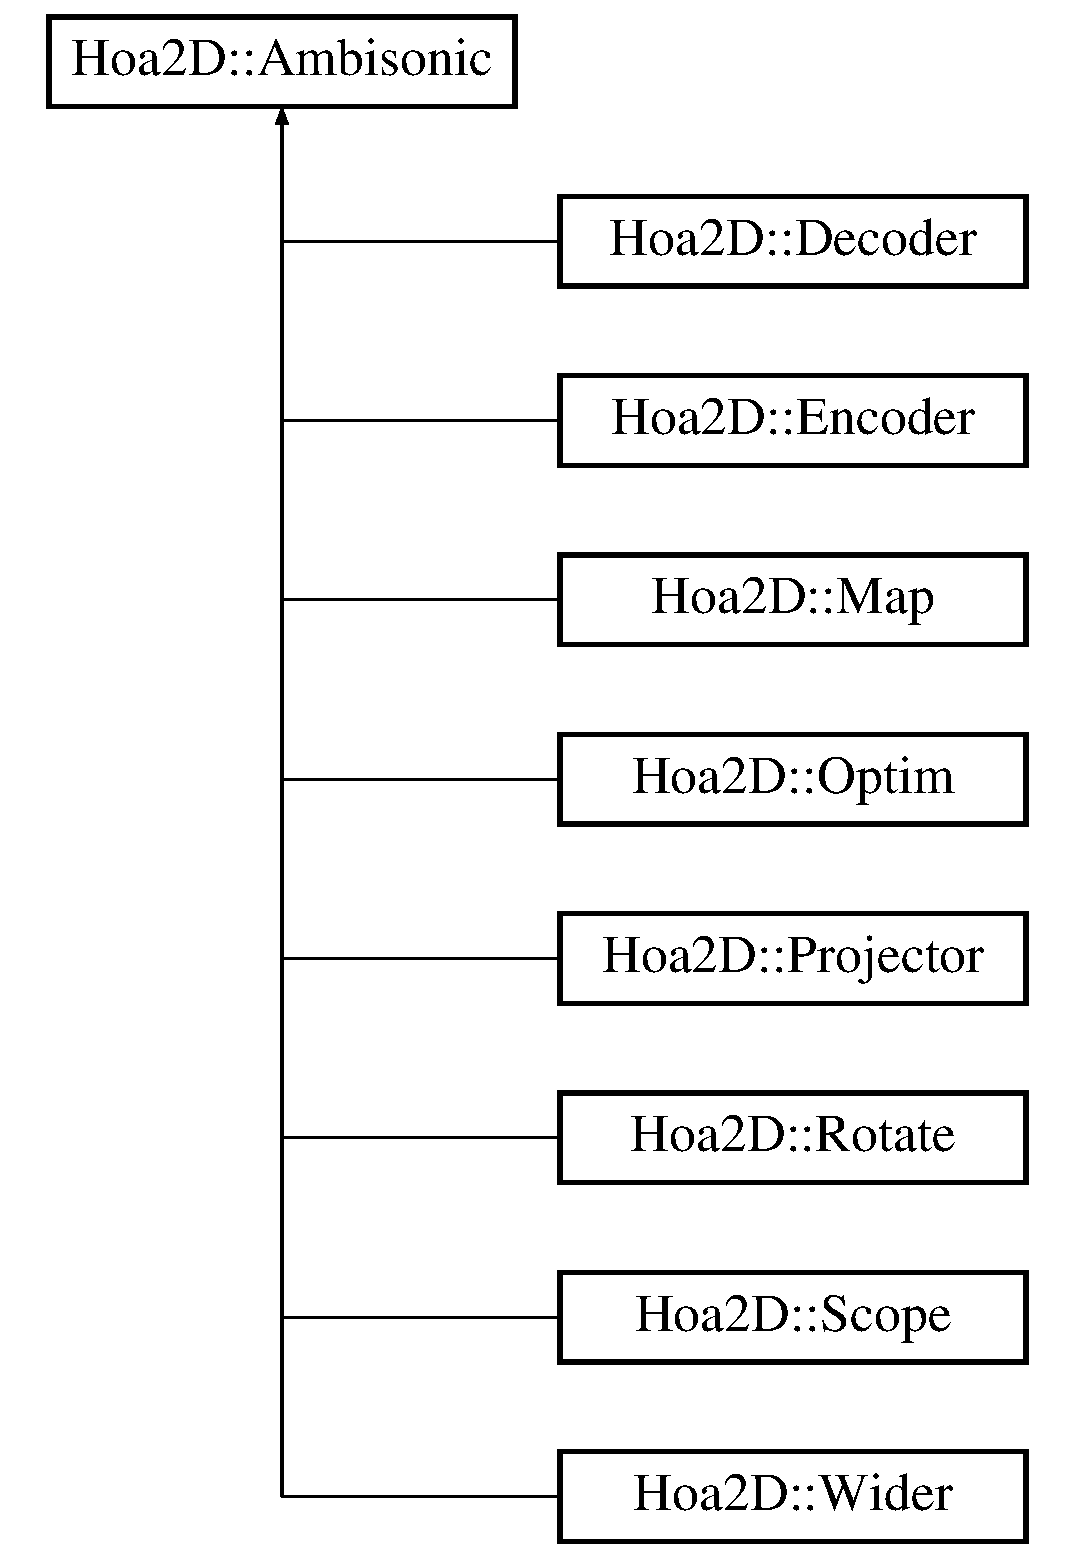
\includegraphics[height=12.000000cm]{class_hoa2_d_1_1_ambisonic}
\end{center}
\end{figure}
\subsection*{Public Member Functions}
\begin{DoxyCompactItemize}
\item 
\hyperlink{class_hoa2_d_1_1_ambisonic_ac53cc3ea0b6600dd84d761f89b5af9d3}{Ambisonic} (unsigned int order)
\begin{DoxyCompactList}\small\item\em The ambisonic constructor. \end{DoxyCompactList}\item 
\hyperlink{class_hoa2_d_1_1_ambisonic_a27be996cfb2bad88e13a32c0d7dba517}{$\sim$\-Ambisonic} ()
\item 
unsigned int \hyperlink{class_hoa2_d_1_1_ambisonic_a00797f96b864e2913567e08239ed9593}{get\-Order} () const 
\item 
unsigned int \hyperlink{class_hoa2_d_1_1_ambisonic_ae7cee18218c9bf00091d83e661d487ee}{get\-Number\-Of\-Harmonics} () const 
\item 
long \hyperlink{class_hoa2_d_1_1_ambisonic_a68c389087fb999101a499f6849b635f9}{get\-Harmonic\-Argument} (unsigned int index) const 
\begin{DoxyCompactList}\small\item\em Retrieve the argument of an harmonic. \end{DoxyCompactList}\item 
long \hyperlink{class_hoa2_d_1_1_ambisonic_a9485abf2b4f1b1aec8d0da9b12cf42ed}{get\-Harmonic\-Band} (unsigned int index) const 
\begin{DoxyCompactList}\small\item\em Retrieve the band of an harmonic. \end{DoxyCompactList}\item 
std\-::string \hyperlink{class_hoa2_d_1_1_ambisonic_a6b6f6ff74792f00bf5095dc9cfec28a4}{get\-Harmonics\-Name} (unsigned int index) const 
\begin{DoxyCompactList}\small\item\em Retrieve a name for an harmonic. \end{DoxyCompactList}\end{DoxyCompactItemize}


\subsection{Detailed Description}
The ambisonic class. 

Most of the ambisonic classes inherit from this classe. It computes the number of harmonics, their arguments and their orders depending of the decomposition order. etc... 

Definition at line 18 of file Ambisonic.\-h.



\subsection{Constructor \& Destructor Documentation}
\hypertarget{class_hoa2_d_1_1_ambisonic_ac53cc3ea0b6600dd84d761f89b5af9d3}{\index{Hoa2\-D\-::\-Ambisonic@{Hoa2\-D\-::\-Ambisonic}!Ambisonic@{Ambisonic}}
\index{Ambisonic@{Ambisonic}!Hoa2D::Ambisonic@{Hoa2\-D\-::\-Ambisonic}}
\subsubsection[{Ambisonic}]{\setlength{\rightskip}{0pt plus 5cm}Hoa2\-D\-::\-Ambisonic\-::\-Ambisonic (
\begin{DoxyParamCaption}
\item[{unsigned int}]{order}
\end{DoxyParamCaption}
)}}\label{class_hoa2_d_1_1_ambisonic_ac53cc3ea0b6600dd84d761f89b5af9d3}


The ambisonic constructor. 

The ambisonic constructor allocates and initializes the generale member values depending of a decomposition order. 
\begin{DoxyParams}{Parameters}
{\em order} & The order, must be at least 1. \\
\hline
\end{DoxyParams}


Definition at line 11 of file Ambisonic.\-cpp.

\hypertarget{class_hoa2_d_1_1_ambisonic_a27be996cfb2bad88e13a32c0d7dba517}{\index{Hoa2\-D\-::\-Ambisonic@{Hoa2\-D\-::\-Ambisonic}!$\sim$\-Ambisonic@{$\sim$\-Ambisonic}}
\index{$\sim$\-Ambisonic@{$\sim$\-Ambisonic}!Hoa2D::Ambisonic@{Hoa2\-D\-::\-Ambisonic}}
\subsubsection[{$\sim$\-Ambisonic}]{\setlength{\rightskip}{0pt plus 5cm}Hoa2\-D\-::\-Ambisonic\-::$\sim$\-Ambisonic (
\begin{DoxyParamCaption}
{}
\end{DoxyParamCaption}
)}}\label{class_hoa2_d_1_1_ambisonic_a27be996cfb2bad88e13a32c0d7dba517}
The ambisonic destructor. 

Definition at line 25 of file Ambisonic.\-cpp.



\subsection{Member Function Documentation}
\hypertarget{class_hoa2_d_1_1_ambisonic_a68c389087fb999101a499f6849b635f9}{\index{Hoa2\-D\-::\-Ambisonic@{Hoa2\-D\-::\-Ambisonic}!get\-Harmonic\-Argument@{get\-Harmonic\-Argument}}
\index{get\-Harmonic\-Argument@{get\-Harmonic\-Argument}!Hoa2D::Ambisonic@{Hoa2\-D\-::\-Ambisonic}}
\subsubsection[{get\-Harmonic\-Argument}]{\setlength{\rightskip}{0pt plus 5cm}long Hoa2\-D\-::\-Ambisonic\-::get\-Harmonic\-Argument (
\begin{DoxyParamCaption}
\item[{unsigned int}]{index}
\end{DoxyParamCaption}
) const\hspace{0.3cm}{\ttfamily [inline]}}}\label{class_hoa2_d_1_1_ambisonic_a68c389087fb999101a499f6849b635f9}


Retrieve the argument of an harmonic. 

The argument of an harmonic is in the range -\/order to order. The harmonics are sorted by their bands, from 0 to the decomposition order and, in each band, there are the 2 harmonics with the arguments -\/band and band. For the first bands, the harmonics arrangement is h\mbox{[}0\mbox{]} h\mbox{[}-\/1\mbox{]} h\mbox{[}1\mbox{]} h\mbox{[}-\/2\mbox{]} h\mbox{[}2\mbox{]} h\mbox{[}-\/3\mbox{]} h\mbox{[}3\mbox{]}etc. with h\mbox{[}argument\mbox{]}.


\begin{DoxyParams}{Parameters}
{\em index} & The index of an harmonic. \\
\hline
\end{DoxyParams}
\begin{DoxyReturn}{Returns}
The method returns the argument of the harmonic if the harmonic exists, otherwise the function generates an error. 
\end{DoxyReturn}
\begin{DoxySeeAlso}{See Also}
\hyperlink{class_hoa2_d_1_1_ambisonic_a9485abf2b4f1b1aec8d0da9b12cf42ed}{get\-Harmonic\-Band()} 

\hyperlink{class_hoa2_d_1_1_ambisonic_a6b6f6ff74792f00bf5095dc9cfec28a4}{get\-Harmonics\-Name()} 
\end{DoxySeeAlso}


Definition at line 58 of file Ambisonic.\-h.

\hypertarget{class_hoa2_d_1_1_ambisonic_a9485abf2b4f1b1aec8d0da9b12cf42ed}{\index{Hoa2\-D\-::\-Ambisonic@{Hoa2\-D\-::\-Ambisonic}!get\-Harmonic\-Band@{get\-Harmonic\-Band}}
\index{get\-Harmonic\-Band@{get\-Harmonic\-Band}!Hoa2D::Ambisonic@{Hoa2\-D\-::\-Ambisonic}}
\subsubsection[{get\-Harmonic\-Band}]{\setlength{\rightskip}{0pt plus 5cm}long Hoa2\-D\-::\-Ambisonic\-::get\-Harmonic\-Band (
\begin{DoxyParamCaption}
\item[{unsigned int}]{index}
\end{DoxyParamCaption}
) const\hspace{0.3cm}{\ttfamily [inline]}}}\label{class_hoa2_d_1_1_ambisonic_a9485abf2b4f1b1aec8d0da9b12cf42ed}


Retrieve the band of an harmonic. 

The bands of the harmonics are in the range 0 to the decomposition order. Each band contains 2 harmonics with the arguments -\/band and band. For the first bands, the harmonics arrangement is h\mbox{[}0\mbox{]} h\mbox{[}-\/1\mbox{]} h\mbox{[}1\mbox{]} h\mbox{[}-\/2\mbox{]} h\mbox{[}2\mbox{]} h\mbox{[}-\/3\mbox{]} h\mbox{[}3\mbox{]}, etc. with h\mbox{[}argument\mbox{]}.


\begin{DoxyParams}{Parameters}
{\em index} & The index of an harmonic. \\
\hline
\end{DoxyParams}
\begin{DoxyReturn}{Returns}
The method returns the band of the harmonic if the harmonic exists, otherwise the function generates an error. 
\end{DoxyReturn}
\begin{DoxySeeAlso}{See Also}
\hyperlink{class_hoa2_d_1_1_ambisonic_a68c389087fb999101a499f6849b635f9}{get\-Harmonic\-Argument()} 

\hyperlink{class_hoa2_d_1_1_ambisonic_a6b6f6ff74792f00bf5095dc9cfec28a4}{get\-Harmonics\-Name()} 
\end{DoxySeeAlso}


Definition at line 72 of file Ambisonic.\-h.

\hypertarget{class_hoa2_d_1_1_ambisonic_a6b6f6ff74792f00bf5095dc9cfec28a4}{\index{Hoa2\-D\-::\-Ambisonic@{Hoa2\-D\-::\-Ambisonic}!get\-Harmonics\-Name@{get\-Harmonics\-Name}}
\index{get\-Harmonics\-Name@{get\-Harmonics\-Name}!Hoa2D::Ambisonic@{Hoa2\-D\-::\-Ambisonic}}
\subsubsection[{get\-Harmonics\-Name}]{\setlength{\rightskip}{0pt plus 5cm}std\-::string Hoa2\-D\-::\-Ambisonic\-::get\-Harmonics\-Name (
\begin{DoxyParamCaption}
\item[{unsigned int}]{index}
\end{DoxyParamCaption}
) const\hspace{0.3cm}{\ttfamily [inline]}}}\label{class_hoa2_d_1_1_ambisonic_a6b6f6ff74792f00bf5095dc9cfec28a4}


Retrieve a name for an harmonic. 

Retrieve a name for an harmonic in a std\-::string format that will be \char`\"{}harmonic argument\char`\"{}.


\begin{DoxyParams}{Parameters}
{\em index} & The index of an harmonic. \\
\hline
\end{DoxyParams}
\begin{DoxyReturn}{Returns}
The method returns a name for the harmonic that contains its argument if the harmonic exists, otherwise the function generates an error.
\end{DoxyReturn}
\begin{DoxySeeAlso}{See Also}
\hyperlink{class_hoa2_d_1_1_ambisonic_a9485abf2b4f1b1aec8d0da9b12cf42ed}{get\-Harmonic\-Band()} 

\hyperlink{class_hoa2_d_1_1_ambisonic_a68c389087fb999101a499f6849b635f9}{get\-Harmonic\-Argument()} 
\end{DoxySeeAlso}


Definition at line 87 of file Ambisonic.\-h.

\hypertarget{class_hoa2_d_1_1_ambisonic_ae7cee18218c9bf00091d83e661d487ee}{\index{Hoa2\-D\-::\-Ambisonic@{Hoa2\-D\-::\-Ambisonic}!get\-Number\-Of\-Harmonics@{get\-Number\-Of\-Harmonics}}
\index{get\-Number\-Of\-Harmonics@{get\-Number\-Of\-Harmonics}!Hoa2D::Ambisonic@{Hoa2\-D\-::\-Ambisonic}}
\subsubsection[{get\-Number\-Of\-Harmonics}]{\setlength{\rightskip}{0pt plus 5cm}unsigned int Hoa2\-D\-::\-Ambisonic\-::get\-Number\-Of\-Harmonics (
\begin{DoxyParamCaption}
{}
\end{DoxyParamCaption}
) const\hspace{0.3cm}{\ttfamily [inline]}}}\label{class_hoa2_d_1_1_ambisonic_ae7cee18218c9bf00091d83e661d487ee}
Retrieve the number of harmonics. 

Definition at line 45 of file Ambisonic.\-h.

\hypertarget{class_hoa2_d_1_1_ambisonic_a00797f96b864e2913567e08239ed9593}{\index{Hoa2\-D\-::\-Ambisonic@{Hoa2\-D\-::\-Ambisonic}!get\-Order@{get\-Order}}
\index{get\-Order@{get\-Order}!Hoa2D::Ambisonic@{Hoa2\-D\-::\-Ambisonic}}
\subsubsection[{get\-Order}]{\setlength{\rightskip}{0pt plus 5cm}unsigned int Hoa2\-D\-::\-Ambisonic\-::get\-Order (
\begin{DoxyParamCaption}
{}
\end{DoxyParamCaption}
) const\hspace{0.3cm}{\ttfamily [inline]}}}\label{class_hoa2_d_1_1_ambisonic_a00797f96b864e2913567e08239ed9593}
Retrieve the decomposition order. 

Definition at line 38 of file Ambisonic.\-h.



The documentation for this class was generated from the following files\-:\begin{DoxyCompactItemize}
\item 
/\-Users/elioton/\-Documents/programmation/\-C\-I\-C\-M/source\-Tree/\-Hoa\-Library/\-Sources/\-Hoa2\-D/Ambisonic.\-h\item 
/\-Users/elioton/\-Documents/programmation/\-C\-I\-C\-M/source\-Tree/\-Hoa\-Library/\-Sources/\-Hoa2\-D/Ambisonic.\-cpp\end{DoxyCompactItemize}

\hypertarget{class_hoa3_d_1_1_ambisonic}{\section{Hoa3\-D\-:\-:Ambisonic Class Reference}
\label{class_hoa3_d_1_1_ambisonic}\index{Hoa3\-D\-::\-Ambisonic@{Hoa3\-D\-::\-Ambisonic}}
}


The ambisonic class.  




{\ttfamily \#include $<$Hoa3\-D\-Ambisonic.\-h$>$}

Inheritance diagram for Hoa3\-D\-:\-:Ambisonic\-:\begin{figure}[H]
\begin{center}
\leavevmode
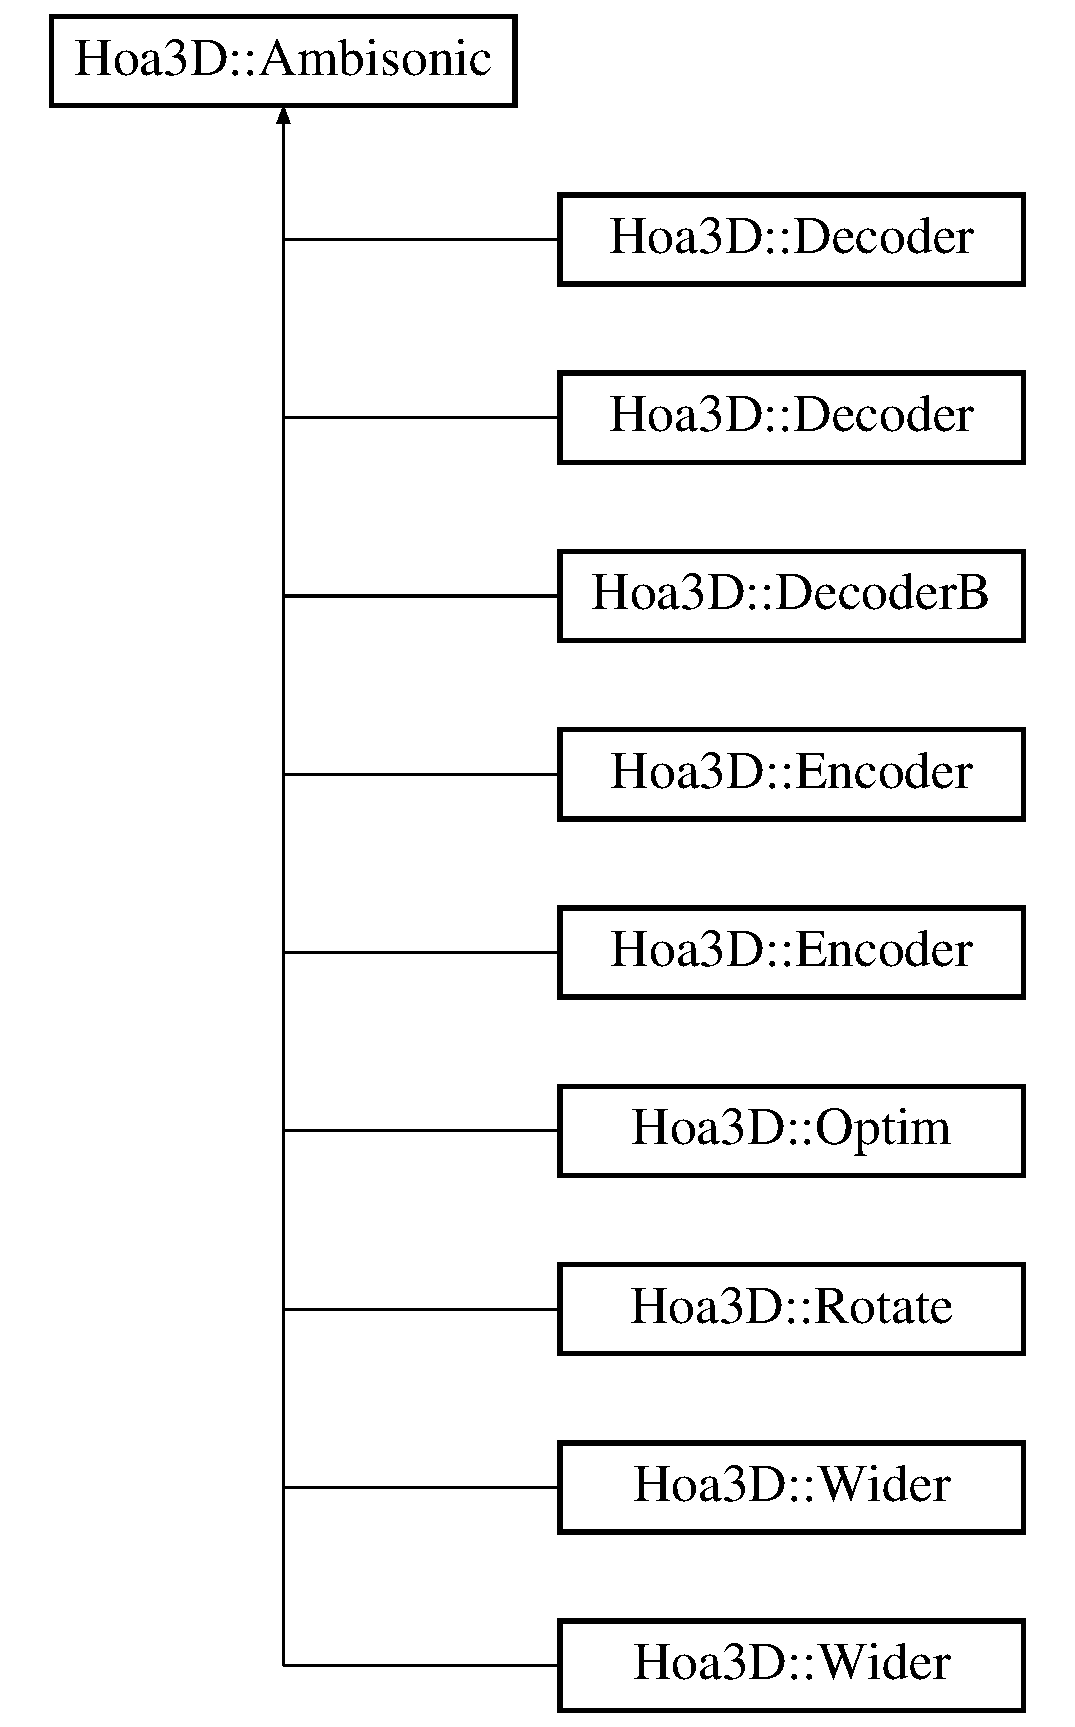
\includegraphics[height=2.000000cm]{class_hoa3_d_1_1_ambisonic}
\end{center}
\end{figure}
\subsection*{Public Member Functions}
\begin{DoxyCompactItemize}
\item 
\hyperlink{class_hoa3_d_1_1_ambisonic_aedbcac4a5b11cec6738e1047ecee7e7b}{Ambisonic} (unsigned int order=1)
\begin{DoxyCompactList}\small\item\em The ambisonic constructor. \end{DoxyCompactList}\item 
\hyperlink{class_hoa3_d_1_1_ambisonic_a082fc2e3f9910703ddb49b9a478329bf}{$\sim$\-Ambisonic} ()
\item 
long \hyperlink{class_hoa3_d_1_1_ambisonic_a677405a1c3aa359753bd675d4614e7da}{get\-Order} ()
\item 
long \hyperlink{class_hoa3_d_1_1_ambisonic_aa9d613f38e6876326201995a5a415410}{get\-Number\-Of\-Harmonics} ()
\item 
long \hyperlink{class_hoa3_d_1_1_ambisonic_af03625afb9f21ef3574eafa8501129b4}{get\-Number\-Of\-Inputs} ()
\item 
long \hyperlink{class_hoa3_d_1_1_ambisonic_a126ed3be1aa3d155f56ca75ca3d69de5}{get\-Number\-Of\-Outputs} ()
\item 
long \hyperlink{class_hoa3_d_1_1_ambisonic_a3acaabfd013671c94e057e23eea1d068}{get\-Harmonic\-Argument} (unsigned int index)
\begin{DoxyCompactList}\small\item\em Retrieve the argument of an harmonic. \end{DoxyCompactList}\item 
long \hyperlink{class_hoa3_d_1_1_ambisonic_a06ecceb7aef44cd7008fd8beaf8cf33e}{get\-Harmonic\-Band} (unsigned int index)
\begin{DoxyCompactList}\small\item\em Retrieve the band of an harmonic. \end{DoxyCompactList}\item 
std\-::string \hyperlink{class_hoa3_d_1_1_ambisonic_a1b4578538f4fd0d311102b2f3ec4dac6}{get\-Harmonics\-Name} (unsigned int index)
\begin{DoxyCompactList}\small\item\em Retrieve a good name for an harmonic. \end{DoxyCompactList}\end{DoxyCompactItemize}


\subsection{Detailed Description}
The ambisonic class. 

Most of the ambisonic classes inherit from this classe. It computes the number of harmonics, their indices and their orders depending of the decomposition order. etc... 

\subsection{Constructor \& Destructor Documentation}
\hypertarget{class_hoa3_d_1_1_ambisonic_aedbcac4a5b11cec6738e1047ecee7e7b}{\index{Hoa3\-D\-::\-Ambisonic@{Hoa3\-D\-::\-Ambisonic}!Ambisonic@{Ambisonic}}
\index{Ambisonic@{Ambisonic}!Hoa3D::Ambisonic@{Hoa3\-D\-::\-Ambisonic}}
\subsubsection[{Ambisonic}]{\setlength{\rightskip}{0pt plus 5cm}Ambisonic\-::\-Ambisonic (
\begin{DoxyParamCaption}
\item[{unsigned int}]{order = {\ttfamily 1}}
\end{DoxyParamCaption}
)}}\label{class_hoa3_d_1_1_ambisonic_aedbcac4a5b11cec6738e1047ecee7e7b}


The ambisonic constructor. 

The ambisonic constructor allocates and initializes the generale member values depending of a decomposition order. 
\begin{DoxyParams}{Parameters}
{\em order} & The order, must be at least 1. \\
\hline
\end{DoxyParams}
\hypertarget{class_hoa3_d_1_1_ambisonic_a082fc2e3f9910703ddb49b9a478329bf}{\index{Hoa3\-D\-::\-Ambisonic@{Hoa3\-D\-::\-Ambisonic}!$\sim$\-Ambisonic@{$\sim$\-Ambisonic}}
\index{$\sim$\-Ambisonic@{$\sim$\-Ambisonic}!Hoa3D::Ambisonic@{Hoa3\-D\-::\-Ambisonic}}
\subsubsection[{$\sim$\-Ambisonic}]{\setlength{\rightskip}{0pt plus 5cm}Ambisonic\-::$\sim$\-Ambisonic (
\begin{DoxyParamCaption}
{}
\end{DoxyParamCaption}
)}}\label{class_hoa3_d_1_1_ambisonic_a082fc2e3f9910703ddb49b9a478329bf}
The ambisonic destructor. 

\subsection{Member Function Documentation}
\hypertarget{class_hoa3_d_1_1_ambisonic_a3acaabfd013671c94e057e23eea1d068}{\index{Hoa3\-D\-::\-Ambisonic@{Hoa3\-D\-::\-Ambisonic}!get\-Harmonic\-Argument@{get\-Harmonic\-Argument}}
\index{get\-Harmonic\-Argument@{get\-Harmonic\-Argument}!Hoa3D::Ambisonic@{Hoa3\-D\-::\-Ambisonic}}
\subsubsection[{get\-Harmonic\-Argument}]{\setlength{\rightskip}{0pt plus 5cm}long Ambisonic\-::get\-Harmonic\-Argument (
\begin{DoxyParamCaption}
\item[{unsigned int}]{index}
\end{DoxyParamCaption}
)}}\label{class_hoa3_d_1_1_ambisonic_a3acaabfd013671c94e057e23eea1d068}


Retrieve the argument of an harmonic. 

The argument of an harmonic is in the range -\/band to band. The harmonics are sorted by their bands, from 0 to the decomposition order and, in each band, they are sorted by their arguments in the range -\/band to band. For the first bands, the harmonics arrangement is h\mbox{[}0, 0\mbox{]} h\mbox{[}1, -\/1\mbox{]} h\mbox{[}1, 0\mbox{]} h\mbox{[}1, 1\mbox{]} h\mbox{[}2, -\/2\mbox{]} h\mbox{[}2, -\/1\mbox{]} h\mbox{[}2, 0\mbox{]} h\mbox{[}2, 1\mbox{]} h\mbox{[}2, 2\mbox{]} etc. with h\mbox{[}band, argument\mbox{]}.


\begin{DoxyParams}{Parameters}
{\em index} & The global index of an harmonic. \\
\hline
\end{DoxyParams}
\begin{DoxyReturn}{Returns}
The method returns the argument of an harmonic or 0 if the harmonic does not exist. 
\end{DoxyReturn}
\begin{DoxySeeAlso}{See Also}
\hyperlink{class_hoa3_d_1_1_ambisonic_a06ecceb7aef44cd7008fd8beaf8cf33e}{get\-Harmonic\-Band()} 
\end{DoxySeeAlso}
\hypertarget{class_hoa3_d_1_1_ambisonic_a06ecceb7aef44cd7008fd8beaf8cf33e}{\index{Hoa3\-D\-::\-Ambisonic@{Hoa3\-D\-::\-Ambisonic}!get\-Harmonic\-Band@{get\-Harmonic\-Band}}
\index{get\-Harmonic\-Band@{get\-Harmonic\-Band}!Hoa3D::Ambisonic@{Hoa3\-D\-::\-Ambisonic}}
\subsubsection[{get\-Harmonic\-Band}]{\setlength{\rightskip}{0pt plus 5cm}long Ambisonic\-::get\-Harmonic\-Band (
\begin{DoxyParamCaption}
\item[{unsigned int}]{index}
\end{DoxyParamCaption}
)}}\label{class_hoa3_d_1_1_ambisonic_a06ecceb7aef44cd7008fd8beaf8cf33e}


Retrieve the band of an harmonic. 

The bands of the harmonics are in the range 0 to the decomposition order. Each band contains 2 $\ast$ band + 1 harmonics in the range -\/band to band. For the first bands, the harmonics arrangement is h\mbox{[}0, 0\mbox{]} h\mbox{[}1, -\/1\mbox{]} h\mbox{[}1, 0\mbox{]} h\mbox{[}1, 1\mbox{]} h\mbox{[}2, -\/2\mbox{]} h\mbox{[}2, -\/1\mbox{]} h\mbox{[}2, 0\mbox{]} h\mbox{[}2, 1\mbox{]} h\mbox{[}2, 2\mbox{]} etc. with h\mbox{[}band, argument\mbox{]}.


\begin{DoxyParams}{Parameters}
{\em index} & The global index of an harmonic. \\
\hline
\end{DoxyParams}
\begin{DoxyReturn}{Returns}
The method returns the band of an harmonic or 0 if the harmonic does not exist. 
\end{DoxyReturn}
\begin{DoxySeeAlso}{See Also}
\hyperlink{class_hoa3_d_1_1_ambisonic_a3acaabfd013671c94e057e23eea1d068}{get\-Harmonic\-Argument()} 
\end{DoxySeeAlso}
\hypertarget{class_hoa3_d_1_1_ambisonic_a1b4578538f4fd0d311102b2f3ec4dac6}{\index{Hoa3\-D\-::\-Ambisonic@{Hoa3\-D\-::\-Ambisonic}!get\-Harmonics\-Name@{get\-Harmonics\-Name}}
\index{get\-Harmonics\-Name@{get\-Harmonics\-Name}!Hoa3D::Ambisonic@{Hoa3\-D\-::\-Ambisonic}}
\subsubsection[{get\-Harmonics\-Name}]{\setlength{\rightskip}{0pt plus 5cm}std\-::string Ambisonic\-::get\-Harmonics\-Name (
\begin{DoxyParamCaption}
\item[{unsigned int}]{index}
\end{DoxyParamCaption}
)}}\label{class_hoa3_d_1_1_ambisonic_a1b4578538f4fd0d311102b2f3ec4dac6}


Retrieve a good name for an harmonic. 

Retrieve a good name for an harmonic.


\begin{DoxyParams}{Parameters}
{\em index} & The global index of an harmonic. \\
\hline
\end{DoxyParams}
\hypertarget{class_hoa3_d_1_1_ambisonic_aa9d613f38e6876326201995a5a415410}{\index{Hoa3\-D\-::\-Ambisonic@{Hoa3\-D\-::\-Ambisonic}!get\-Number\-Of\-Harmonics@{get\-Number\-Of\-Harmonics}}
\index{get\-Number\-Of\-Harmonics@{get\-Number\-Of\-Harmonics}!Hoa3D::Ambisonic@{Hoa3\-D\-::\-Ambisonic}}
\subsubsection[{get\-Number\-Of\-Harmonics}]{\setlength{\rightskip}{0pt plus 5cm}long Ambisonic\-::get\-Number\-Of\-Harmonics (
\begin{DoxyParamCaption}
{}
\end{DoxyParamCaption}
)}}\label{class_hoa3_d_1_1_ambisonic_aa9d613f38e6876326201995a5a415410}
Retrieve the number of harmonics. \hypertarget{class_hoa3_d_1_1_ambisonic_af03625afb9f21ef3574eafa8501129b4}{\index{Hoa3\-D\-::\-Ambisonic@{Hoa3\-D\-::\-Ambisonic}!get\-Number\-Of\-Inputs@{get\-Number\-Of\-Inputs}}
\index{get\-Number\-Of\-Inputs@{get\-Number\-Of\-Inputs}!Hoa3D::Ambisonic@{Hoa3\-D\-::\-Ambisonic}}
\subsubsection[{get\-Number\-Of\-Inputs}]{\setlength{\rightskip}{0pt plus 5cm}long Ambisonic\-::get\-Number\-Of\-Inputs (
\begin{DoxyParamCaption}
{}
\end{DoxyParamCaption}
)}}\label{class_hoa3_d_1_1_ambisonic_af03625afb9f21ef3574eafa8501129b4}
Retrieve the number of inputs. \hypertarget{class_hoa3_d_1_1_ambisonic_a126ed3be1aa3d155f56ca75ca3d69de5}{\index{Hoa3\-D\-::\-Ambisonic@{Hoa3\-D\-::\-Ambisonic}!get\-Number\-Of\-Outputs@{get\-Number\-Of\-Outputs}}
\index{get\-Number\-Of\-Outputs@{get\-Number\-Of\-Outputs}!Hoa3D::Ambisonic@{Hoa3\-D\-::\-Ambisonic}}
\subsubsection[{get\-Number\-Of\-Outputs}]{\setlength{\rightskip}{0pt plus 5cm}long Ambisonic\-::get\-Number\-Of\-Outputs (
\begin{DoxyParamCaption}
{}
\end{DoxyParamCaption}
)}}\label{class_hoa3_d_1_1_ambisonic_a126ed3be1aa3d155f56ca75ca3d69de5}
Retrieve the number of outputs. \hypertarget{class_hoa3_d_1_1_ambisonic_a677405a1c3aa359753bd675d4614e7da}{\index{Hoa3\-D\-::\-Ambisonic@{Hoa3\-D\-::\-Ambisonic}!get\-Order@{get\-Order}}
\index{get\-Order@{get\-Order}!Hoa3D::Ambisonic@{Hoa3\-D\-::\-Ambisonic}}
\subsubsection[{get\-Order}]{\setlength{\rightskip}{0pt plus 5cm}long Ambisonic\-::get\-Order (
\begin{DoxyParamCaption}
{}
\end{DoxyParamCaption}
)}}\label{class_hoa3_d_1_1_ambisonic_a677405a1c3aa359753bd675d4614e7da}
Retrieve the decomposition order. 

The documentation for this class was generated from the following files\-:\begin{DoxyCompactItemize}
\item 
/\-Users/\-Pierre/\-Source\-Tree/\-Hoa\-Library/\-Sources/hoa\-Ambisonics/Hoa3\-D\-Ambisonic.\-h\item 
/\-Users/\-Pierre/\-Source\-Tree/\-Hoa\-Library/\-Sources/hoa\-Ambisonics/Hoa3\-D\-Ambisonic.\-cpp\end{DoxyCompactItemize}

\hypertarget{class_ambisonics_meter}{\section{Ambisonics\-Meter Class Reference}
\label{class_ambisonics_meter}\index{Ambisonics\-Meter@{Ambisonics\-Meter}}
}


{\ttfamily \#include $<$Ambisonics\-Meter.\-h$>$}

Inheritance diagram for Ambisonics\-Meter\-:\begin{figure}[H]
\begin{center}
\leavevmode
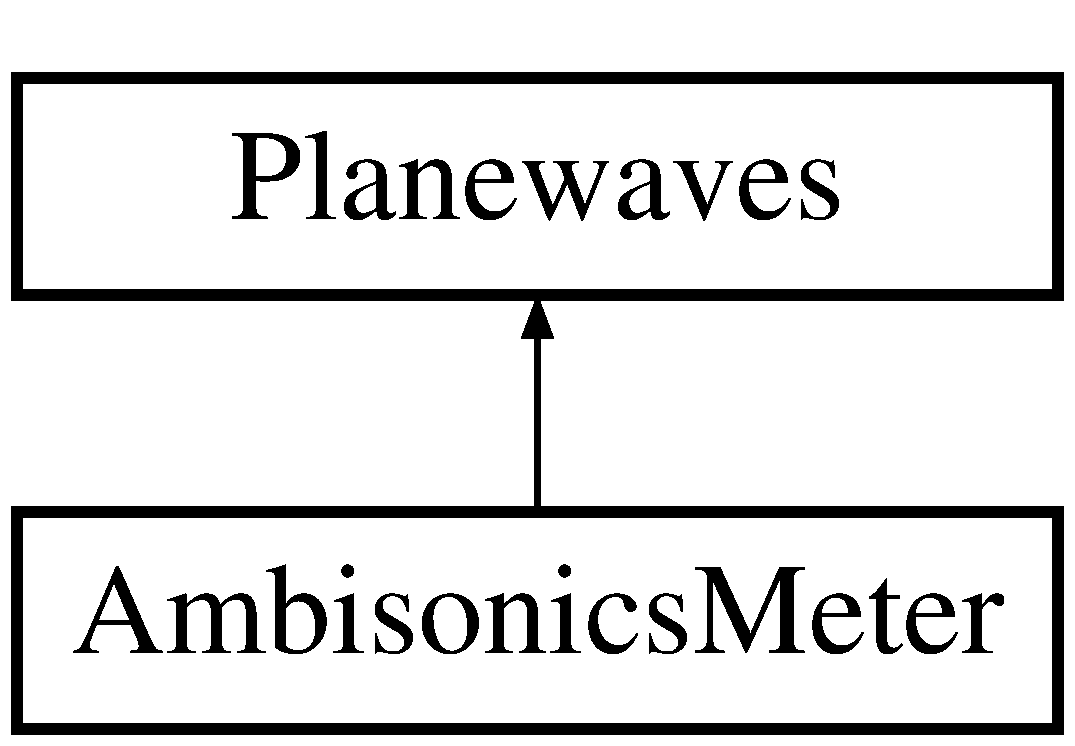
\includegraphics[height=2.000000cm]{class_ambisonics_meter}
\end{center}
\end{figure}
\subsection*{Public Member Functions}
\begin{DoxyCompactItemize}
\item 
\hyperlink{class_ambisonics_meter_ab6652775a732fc5d190101e5673c6758}{Ambisonics\-Meter} (long a\-Number\-Of\-Channel=1, long a\-Vector\-Size=0, double a\-Sampling\-Rate=44100.)
\item 
\hypertarget{class_ambisonics_meter_a67dcdc08682898d4460cf8e04f53a201}{void {\bfseries set\-Number\-Of\-Loudspeakers} (long a\-Number\-Of\-Channels)}\label{class_ambisonics_meter_a67dcdc08682898d4460cf8e04f53a201}

\item 
\hypertarget{class_ambisonics_meter_a14720821cf28453bc1609a234121c040}{void {\bfseries set\-Vector\-Size} (long a\-Vector\-Size)}\label{class_ambisonics_meter_a14720821cf28453bc1609a234121c040}

\item 
\hypertarget{class_ambisonics_meter_a991f4c9b08bf47e0eb10fda9e907f511}{void {\bfseries set\-Loudspeaker\-Angle\-Degrees} (long an\-Index, double an\-Angle)}\label{class_ambisonics_meter_a991f4c9b08bf47e0eb10fda9e907f511}

\item 
\hypertarget{class_ambisonics_meter_a58425860d8afb4eb62328833e68baf12}{void {\bfseries set\-Loudspeaker\-Angles\-Degrees} (long a\-Size, double $\ast$angles)}\label{class_ambisonics_meter_a58425860d8afb4eb62328833e68baf12}

\item 
\hypertarget{class_ambisonics_meter_a15bbfeebc227c01a4041316905e051c7}{double {\bfseries get\-Loudspeaker\-Peaks} (long an\-Index)}\label{class_ambisonics_meter_a15bbfeebc227c01a4041316905e051c7}

\item 
\hypertarget{class_ambisonics_meter_a2a1f8138c0b030eeb3f83a536c72e6e4}{double {\bfseries get\-Loudspeaker\-Energy} (long an\-Index)}\label{class_ambisonics_meter_a2a1f8138c0b030eeb3f83a536c72e6e4}

\item 
\hypertarget{class_ambisonics_meter_a73f0f5db0e7e5e15080d907cddc48e98}{double {\bfseries get\-Energy\-Vector\-Abscissa} ()}\label{class_ambisonics_meter_a73f0f5db0e7e5e15080d907cddc48e98}

\item 
\hypertarget{class_ambisonics_meter_a737f7cf7c2392a3caa50fc79daad1500}{double {\bfseries get\-Energy\-Vector\-Ordinate} ()}\label{class_ambisonics_meter_a737f7cf7c2392a3caa50fc79daad1500}

\item 
\hypertarget{class_ambisonics_meter_a597186413fff3df7e5ee2f82fd0c497a}{double {\bfseries get\-Energy\-Vector\-Angle} ()}\label{class_ambisonics_meter_a597186413fff3df7e5ee2f82fd0c497a}

\item 
\hypertarget{class_ambisonics_meter_a0ed4c04a207ef485252c9075f691be35}{double {\bfseries get\-Energy\-Vector\-Radius} ()}\label{class_ambisonics_meter_a0ed4c04a207ef485252c9075f691be35}

\item 
\hypertarget{class_ambisonics_meter_a1f4ec2a7672144bbeebfedc398e77439}{double {\bfseries get\-Velocity\-Vector\-Abscissa} ()}\label{class_ambisonics_meter_a1f4ec2a7672144bbeebfedc398e77439}

\item 
\hypertarget{class_ambisonics_meter_ab34bc7eff55c357550f05b2852eb6840}{double {\bfseries get\-Velocity\-Vector\-Ordinate} ()}\label{class_ambisonics_meter_ab34bc7eff55c357550f05b2852eb6840}

\item 
\hypertarget{class_ambisonics_meter_a937efec3de37d9702acf18b2b1b00109}{double {\bfseries get\-Velocity\-Vector\-Angle} ()}\label{class_ambisonics_meter_a937efec3de37d9702acf18b2b1b00109}

\item 
\hypertarget{class_ambisonics_meter_a48578aa4790dc7063e9ecb2d37dc66ba}{double {\bfseries get\-Velocity\-Vector\-Radius} ()}\label{class_ambisonics_meter_a48578aa4790dc7063e9ecb2d37dc66ba}

\item 
\hypertarget{class_ambisonics_meter_ad1b0981516635b7773383b498f2a9b39}{double {\bfseries get\-Loudspeaker\-Angle\-Mapped} (long an\-Index)}\label{class_ambisonics_meter_ad1b0981516635b7773383b498f2a9b39}

\item 
\hypertarget{class_ambisonics_meter_a5d01a9986aa9ac1cea65d97c84da49c1}{double {\bfseries get\-Loudspeaker\-Width} (long an\-Index)}\label{class_ambisonics_meter_a5d01a9986aa9ac1cea65d97c84da49c1}

\item 
\hypertarget{class_ambisonics_meter_a72032e205495ad09add249ad65363957}{double {\bfseries get\-Loudspeaker\-Angle\-Radian} (long an\-Index)}\label{class_ambisonics_meter_a72032e205495ad09add249ad65363957}

\item 
\hypertarget{class_ambisonics_meter_ac10c0e4c4c2b3188d084253116edc1b0}{double {\bfseries get\-Loudspeaker\-Angle\-Mapped\-Radian} (long an\-Index)}\label{class_ambisonics_meter_ac10c0e4c4c2b3188d084253116edc1b0}

\item 
\hypertarget{class_ambisonics_meter_a1147487c544561c5865e93603c72f2a3}{double {\bfseries get\-Loudspeaker\-Width\-Radian} (long an\-Index)}\label{class_ambisonics_meter_a1147487c544561c5865e93603c72f2a3}

\item 
\hypertarget{class_ambisonics_meter_aaf6d66a0e5ab0043c7780ee298f7d927}{std\-::string {\bfseries get\-Channel\-Name} (long an\-Index)}\label{class_ambisonics_meter_aaf6d66a0e5ab0043c7780ee298f7d927}

\item 
\hypertarget{class_ambisonics_meter_aec2469b7c4257c8cf14b7fca0638b49b}{void {\bfseries process} (float $\ast$$\ast$inputs)}\label{class_ambisonics_meter_aec2469b7c4257c8cf14b7fca0638b49b}

\item 
\hypertarget{class_ambisonics_meter_a6b25ca0c6429a4ba0462852433b9fd62}{void {\bfseries process} (double $\ast$$\ast$inputs)}\label{class_ambisonics_meter_a6b25ca0c6429a4ba0462852433b9fd62}

\item 
\hypertarget{class_ambisonics_meter_a95b73d96270c11538421b02d9143a567}{void {\bfseries process\-Energy} ()}\label{class_ambisonics_meter_a95b73d96270c11538421b02d9143a567}

\item 
\hypertarget{class_ambisonics_meter_a837f99343b8d0dbf2c01000d419d48ee}{void {\bfseries process\-Vectors} ()}\label{class_ambisonics_meter_a837f99343b8d0dbf2c01000d419d48ee}

\end{DoxyCompactItemize}
\subsection*{Protected Attributes}
\begin{DoxyCompactItemize}
\item 
\hypertarget{class_ambisonics_meter_a851eee4cd189d850b028f75f44aa0fa5}{\hyperlink{class_ambisonic_vector}{Ambisonic\-Vector} $\ast$ {\bfseries m\-\_\-vectors}}\label{class_ambisonics_meter_a851eee4cd189d850b028f75f44aa0fa5}

\item 
\hypertarget{class_ambisonics_meter_aea287908ab29c57db2dd04c4b7e307d5}{cicm\-\_\-vector\-\_\-double {\bfseries m\-\_\-loudspeakers\-\_\-amplitudes}}\label{class_ambisonics_meter_aea287908ab29c57db2dd04c4b7e307d5}

\item 
\hypertarget{class_ambisonics_meter_a27343caf2b62d5e87fa99c4c1a40cd02}{cicm\-\_\-vector\-\_\-double {\bfseries m\-\_\-loudspeakers\-\_\-peaks}}\label{class_ambisonics_meter_a27343caf2b62d5e87fa99c4c1a40cd02}

\item 
\hypertarget{class_ambisonics_meter_a30e5c805ec6f9329b316d32a03969c67}{cicm\-\_\-vector\-\_\-double {\bfseries m\-\_\-loudspeakers\-\_\-energies}}\label{class_ambisonics_meter_a30e5c805ec6f9329b316d32a03969c67}

\item 
\hypertarget{class_ambisonics_meter_a703b0c4ca60b8ca98a45c15750c5229f}{double {\bfseries m\-\_\-vector\-\_\-coordinates\-\_\-double} \mbox{[}4\mbox{]}}\label{class_ambisonics_meter_a703b0c4ca60b8ca98a45c15750c5229f}

\item 
\hypertarget{class_ambisonics_meter_ac01da8c9577b0fd777a1821946f8b776}{float {\bfseries m\-\_\-vector\-\_\-coordinates\-\_\-float} \mbox{[}4\mbox{]}}\label{class_ambisonics_meter_ac01da8c9577b0fd777a1821946f8b776}

\item 
\hypertarget{class_ambisonics_meter_a82aaf6d19c3a8d7c7f1a52f65b175351}{cicm\-\_\-vector\-\_\-double {\bfseries m\-\_\-loudspeakers\-\_\-angles\-\_\-mapped}}\label{class_ambisonics_meter_a82aaf6d19c3a8d7c7f1a52f65b175351}

\item 
\hypertarget{class_ambisonics_meter_a9fa69f3a2d8bccfb6001bcf6c060b6c1}{cicm\-\_\-vector\-\_\-double {\bfseries m\-\_\-loudspeakers\-\_\-angles\-\_\-width}}\label{class_ambisonics_meter_a9fa69f3a2d8bccfb6001bcf6c060b6c1}

\end{DoxyCompactItemize}
\subsection*{Additional Inherited Members}


\subsection{Detailed Description}
\hyperlink{interface_hoa_library}{Hoa\-Library} \-: A High Order Ambisonics Library Copyright (c) 2012-\/2013 Julien Colafrancesco, Pierre Guillot, Eliott Paris, C\-I\-C\-M, Universite Paris-\/8. All rights reserved.\-re Guillot, C\-I\-C\-M -\/ Université Paris 8 All rights reserved.

Website \-: \href{http://www.mshparisnord.fr/HoaLibrary/}{\tt http\-://www.\-mshparisnord.\-fr/\-Hoa\-Library/} Contacts \-: \href{mailto:cicm.mshparisnord@gmail.com}{\tt cicm.\-mshparisnord@gmail.\-com}

This file is part of H\-O\-A L\-I\-B\-R\-A\-R\-Y.

H\-O\-A L\-I\-B\-R\-A\-R\-Y is free software\-: you can redistribute it and/or modify it under the terms of the G\-N\-U General Public License as published by the Free Software Foundation, either version 3 of the License, or (at your option) any later version.

This program is distributed in the hope that it will be useful, but W\-I\-T\-H\-O\-U\-T A\-N\-Y W\-A\-R\-R\-A\-N\-T\-Y; without even the implied warranty of M\-E\-R\-C\-H\-A\-N\-T\-A\-B\-I\-L\-I\-T\-Y or F\-I\-T\-N\-E\-S\-S F\-O\-R A P\-A\-R\-T\-I\-C\-U\-L\-A\-R P\-U\-R\-P\-O\-S\-E. See the G\-N\-U General Public License for more details.

You should have received a copy of the G\-N\-U General Public License along with this program. If not, see \href{http://www.gnu.org/licenses/}{\tt http\-://www.\-gnu.\-org/licenses/}. 

\subsection{Constructor \& Destructor Documentation}
\hypertarget{class_ambisonics_meter_ab6652775a732fc5d190101e5673c6758}{\index{Ambisonics\-Meter@{Ambisonics\-Meter}!Ambisonics\-Meter@{Ambisonics\-Meter}}
\index{Ambisonics\-Meter@{Ambisonics\-Meter}!AmbisonicsMeter@{Ambisonics\-Meter}}
\subsubsection[{Ambisonics\-Meter}]{\setlength{\rightskip}{0pt plus 5cm}Ambisonics\-Meter\-::\-Ambisonics\-Meter (
\begin{DoxyParamCaption}
\item[{long}]{a\-Number\-Of\-Channels = {\ttfamily 1}, }
\item[{long}]{a\-Vector\-Size = {\ttfamily 0}, }
\item[{double}]{a\-Sampling\-Rate = {\ttfamily 44100.}}
\end{DoxyParamCaption}
)}}\label{class_ambisonics_meter_ab6652775a732fc5d190101e5673c6758}
\hyperlink{interface_hoa_library}{Hoa\-Library} \-: A High Order Ambisonics Library Copyright (c) 2012-\/2013 Julien Colafrancesco, Pierre Guillot, Eliott Paris, C\-I\-C\-M, Universite Paris-\/8. All rights reserved.\-re Guillot, C\-I\-C\-M -\/ Université Paris 8 All rights reserved.

Website \-: \href{http://www.mshparisnord.fr/HoaLibrary/}{\tt http\-://www.\-mshparisnord.\-fr/\-Hoa\-Library/} Contacts \-: \href{mailto:cicm.mshparisnord@gmail.com}{\tt cicm.\-mshparisnord@gmail.\-com}

This file is part of H\-O\-A L\-I\-B\-R\-A\-R\-Y.

H\-O\-A L\-I\-B\-R\-A\-R\-Y is free software\-: you can redistribute it and/or modify it under the terms of the G\-N\-U General Public License as published by the Free Software Foundation, either version 3 of the License, or (at your option) any later version.

This program is distributed in the hope that it will be useful, but W\-I\-T\-H\-O\-U\-T A\-N\-Y W\-A\-R\-R\-A\-N\-T\-Y; without even the implied warranty of M\-E\-R\-C\-H\-A\-N\-T\-A\-B\-I\-L\-I\-T\-Y or F\-I\-T\-N\-E\-S\-S F\-O\-R A P\-A\-R\-T\-I\-C\-U\-L\-A\-R P\-U\-R\-P\-O\-S\-E. See the G\-N\-U General Public License for more details.

You should have received a copy of the G\-N\-U General Public License along with this program. If not, see \href{http://www.gnu.org/licenses/}{\tt http\-://www.\-gnu.\-org/licenses/}. 

The documentation for this class was generated from the following files\-:\begin{DoxyCompactItemize}
\item 
/\-Users/\-Pierre/\-Source\-Tree/\-Hoa\-Library/\-Sources/hoa\-Meter/Ambisonics\-Meter.\-h\item 
/\-Users/\-Pierre/\-Source\-Tree/\-Hoa\-Library/\-Sources/hoa\-Meter/Ambisonics\-Meter.\-cpp\end{DoxyCompactItemize}

\hypertarget{struct_hoa_1_1coordinates_cartesian}{\section{Hoa\-:\-:coordinates\-Cartesian Struct Reference}
\label{struct_hoa_1_1coordinates_cartesian}\index{Hoa\-::coordinates\-Cartesian@{Hoa\-::coordinates\-Cartesian}}
}


\subsection{Detailed Description}


Definition at line 57 of file Hoa\-Defs.\-h.



The documentation for this struct was generated from the following file\-:\begin{DoxyCompactItemize}
\item 
/\-Users/elioton/\-Documents/programmation/\-C\-I\-C\-M/source\-Tree/\-Hoa\-Library/\-Sources/\-Hoa/Hoa\-Defs.\-h\end{DoxyCompactItemize}

\hypertarget{struct_hoa_1_1coordinates_polar}{\section{Hoa\-:\-:coordinates\-Polar Struct Reference}
\label{struct_hoa_1_1coordinates_polar}\index{Hoa\-::coordinates\-Polar@{Hoa\-::coordinates\-Polar}}
}


\subsection{Detailed Description}


Definition at line 51 of file Hoa\-Defs.\-h.



The documentation for this struct was generated from the following file\-:\begin{DoxyCompactItemize}
\item 
/\-Users/elioton/\-Documents/programmation/\-C\-I\-C\-M/source\-Tree/\-Hoa\-Library/\-Sources/\-Hoa/Hoa\-Defs.\-h\end{DoxyCompactItemize}

\hypertarget{class_hoa3_d_1_1_decoder}{\section{Hoa3\-D\-:\-:Decoder Class Reference}
\label{class_hoa3_d_1_1_decoder}\index{Hoa3\-D\-::\-Decoder@{Hoa3\-D\-::\-Decoder}}
}


The ambisonic decoder.  




{\ttfamily \#include $<$Decoder.\-h$>$}

Inheritance diagram for Hoa3\-D\-:\-:Decoder\-:\begin{figure}[H]
\begin{center}
\leavevmode
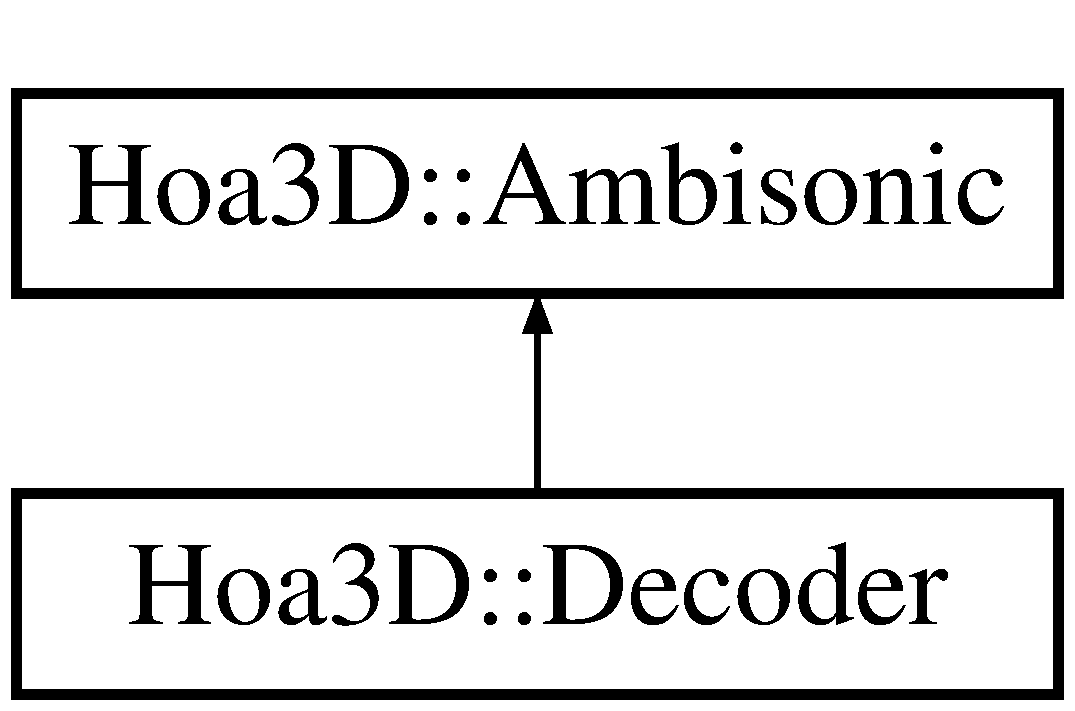
\includegraphics[height=2.000000cm]{class_hoa3_d_1_1_decoder}
\end{center}
\end{figure}
\subsection*{Public Member Functions}
\begin{DoxyCompactItemize}
\item 
\hyperlink{class_hoa3_d_1_1_decoder_aefb3c6a2fd27592480d8198c06ea0968}{Decoder} (unsigned int order, unsigned int number\-Of\-Loudspeakers)
\item 
\hyperlink{class_hoa3_d_1_1_decoder_acc197bebb310a82756ee2061fe371e2d}{$\sim$\-Decoder} ()
\item 
unsigned int \hyperlink{class_hoa3_d_1_1_decoder_a4b14ee0651b397724490de7199d428a7}{get\-Number\-Of\-Loudspeakers} () const 
\begin{DoxyCompactList}\small\item\em This method retrieve the number of loudspeakers. \end{DoxyCompactList}\item 
void \hyperlink{class_hoa3_d_1_1_decoder_ade9c4f54765c1de0f27fadf0b25e88f9}{set\-Loudspeaker\-Position} (unsigned int index, double azimuth, double elevation)
\item 
double \hyperlink{class_hoa3_d_1_1_decoder_a23df7388f6d6b2915566f5aa6d294056}{get\-Loudspeaker\-Azimuth} (unsigned int index) const 
\item 
double \hyperlink{class_hoa3_d_1_1_decoder_aa5102482919297cee85af49991c5984f}{get\-Loudspeaker\-Elevation} (unsigned int index) const 
\item 
void \hyperlink{class_hoa3_d_1_1_decoder_a146f985ebda8e825db2a2ed2cafd5ba6}{process} (const float $\ast$input, float $\ast$output)
\item 
void \hyperlink{class_hoa3_d_1_1_decoder_a2a1931b2fe5c5def0baa9c4d637379a9}{process} (const double $\ast$input, double $\ast$output)
\end{DoxyCompactItemize}


\subsection{Detailed Description}
The ambisonic decoder. 

The decoder should be used to decode a signal encoded in the spherical harmonics domain depending on a decomposition order and a number of loudspeakers. 

Definition at line 18 of file Decoder.\-h.



\subsection{Constructor \& Destructor Documentation}
\hypertarget{class_hoa3_d_1_1_decoder_aefb3c6a2fd27592480d8198c06ea0968}{\index{Hoa3\-D\-::\-Decoder@{Hoa3\-D\-::\-Decoder}!Decoder@{Decoder}}
\index{Decoder@{Decoder}!Hoa3D::Decoder@{Hoa3\-D\-::\-Decoder}}
\subsubsection[{Decoder}]{\setlength{\rightskip}{0pt plus 5cm}Hoa3\-D\-::\-Decoder\-::\-Decoder (
\begin{DoxyParamCaption}
\item[{unsigned int}]{order, }
\item[{unsigned int}]{number\-Of\-Loudspeakers}
\end{DoxyParamCaption}
)}}\label{class_hoa3_d_1_1_decoder_aefb3c6a2fd27592480d8198c06ea0968}
\begin{DoxyVerb}The decoder constructor.
\end{DoxyVerb}
 
\begin{DoxyParams}{Parameters}
{\em order} & The order, must be at least 1. \\
\hline
{\em number\-Of\-Loudspeakers} & The number of loudspeakers, must be at least (order + 1)$^\wedge$2. \\
\hline
{\em shape} & Is a sphere or a half sphere. \\
\hline
\end{DoxyParams}


Definition at line 11 of file Decoder.\-cpp.

\hypertarget{class_hoa3_d_1_1_decoder_acc197bebb310a82756ee2061fe371e2d}{\index{Hoa3\-D\-::\-Decoder@{Hoa3\-D\-::\-Decoder}!$\sim$\-Decoder@{$\sim$\-Decoder}}
\index{$\sim$\-Decoder@{$\sim$\-Decoder}!Hoa3D::Decoder@{Hoa3\-D\-::\-Decoder}}
\subsubsection[{$\sim$\-Decoder}]{\setlength{\rightskip}{0pt plus 5cm}Hoa3\-D\-::\-Decoder\-::$\sim$\-Decoder (
\begin{DoxyParamCaption}
{}
\end{DoxyParamCaption}
)}}\label{class_hoa3_d_1_1_decoder_acc197bebb310a82756ee2061fe371e2d}
The decoder destructor. 

Definition at line 60 of file Decoder.\-cpp.



\subsection{Member Function Documentation}
\hypertarget{class_hoa3_d_1_1_decoder_a23df7388f6d6b2915566f5aa6d294056}{\index{Hoa3\-D\-::\-Decoder@{Hoa3\-D\-::\-Decoder}!get\-Loudspeaker\-Azimuth@{get\-Loudspeaker\-Azimuth}}
\index{get\-Loudspeaker\-Azimuth@{get\-Loudspeaker\-Azimuth}!Hoa3D::Decoder@{Hoa3\-D\-::\-Decoder}}
\subsubsection[{get\-Loudspeaker\-Azimuth}]{\setlength{\rightskip}{0pt plus 5cm}double Hoa3\-D\-::\-Decoder\-::get\-Loudspeaker\-Azimuth (
\begin{DoxyParamCaption}
\item[{unsigned int}]{index}
\end{DoxyParamCaption}
) const}}\label{class_hoa3_d_1_1_decoder_a23df7388f6d6b2915566f5aa6d294056}
\begin{DoxyVerb}Get loudspeaker azimuth value.
\end{DoxyVerb}
 
\begin{DoxyParams}{Parameters}
{\em index} & The index of the loudspeaker. \\
\hline
\end{DoxyParams}
\begin{DoxyReturn}{Returns}
the azimuth value in radians. 
\end{DoxyReturn}
\begin{DoxySeeAlso}{See Also}
\hyperlink{class_hoa3_d_1_1_decoder_aa5102482919297cee85af49991c5984f}{get\-Loudspeaker\-Elevation} 
\end{DoxySeeAlso}


Definition at line 38 of file Decoder.\-cpp.

\hypertarget{class_hoa3_d_1_1_decoder_aa5102482919297cee85af49991c5984f}{\index{Hoa3\-D\-::\-Decoder@{Hoa3\-D\-::\-Decoder}!get\-Loudspeaker\-Elevation@{get\-Loudspeaker\-Elevation}}
\index{get\-Loudspeaker\-Elevation@{get\-Loudspeaker\-Elevation}!Hoa3D::Decoder@{Hoa3\-D\-::\-Decoder}}
\subsubsection[{get\-Loudspeaker\-Elevation}]{\setlength{\rightskip}{0pt plus 5cm}double Hoa3\-D\-::\-Decoder\-::get\-Loudspeaker\-Elevation (
\begin{DoxyParamCaption}
\item[{unsigned int}]{index}
\end{DoxyParamCaption}
) const}}\label{class_hoa3_d_1_1_decoder_aa5102482919297cee85af49991c5984f}
\begin{DoxyVerb}Get loudspeakers elevation value.
\end{DoxyVerb}
 
\begin{DoxyParams}{Parameters}
{\em index} & The index of the loudspeaker. \\
\hline
\end{DoxyParams}
\begin{DoxyReturn}{Returns}
the elevation value in radians. 
\end{DoxyReturn}
\begin{DoxySeeAlso}{See Also}
\hyperlink{class_hoa3_d_1_1_decoder_a23df7388f6d6b2915566f5aa6d294056}{get\-Loudspeaker\-Azimuth} 
\end{DoxySeeAlso}


Definition at line 44 of file Decoder.\-cpp.

\hypertarget{class_hoa3_d_1_1_decoder_a4b14ee0651b397724490de7199d428a7}{\index{Hoa3\-D\-::\-Decoder@{Hoa3\-D\-::\-Decoder}!get\-Number\-Of\-Loudspeakers@{get\-Number\-Of\-Loudspeakers}}
\index{get\-Number\-Of\-Loudspeakers@{get\-Number\-Of\-Loudspeakers}!Hoa3D::Decoder@{Hoa3\-D\-::\-Decoder}}
\subsubsection[{get\-Number\-Of\-Loudspeakers}]{\setlength{\rightskip}{0pt plus 5cm}unsigned int Hoa3\-D\-::\-Decoder\-::get\-Number\-Of\-Loudspeakers (
\begin{DoxyParamCaption}
{}
\end{DoxyParamCaption}
) const\hspace{0.3cm}{\ttfamily [inline]}}}\label{class_hoa3_d_1_1_decoder_a4b14ee0651b397724490de7199d428a7}


This method retrieve the number of loudspeakers. 

Retrieve the number of loudspeakers.

\begin{DoxyReturn}{Returns}
The number of loudspeakers. 
\end{DoxyReturn}


Definition at line 48 of file Decoder.\-h.

\hypertarget{class_hoa3_d_1_1_decoder_a146f985ebda8e825db2a2ed2cafd5ba6}{\index{Hoa3\-D\-::\-Decoder@{Hoa3\-D\-::\-Decoder}!process@{process}}
\index{process@{process}!Hoa3D::Decoder@{Hoa3\-D\-::\-Decoder}}
\subsubsection[{process}]{\setlength{\rightskip}{0pt plus 5cm}void Hoa3\-D\-::\-Decoder\-::process (
\begin{DoxyParamCaption}
\item[{const float $\ast$}]{input, }
\item[{float $\ast$}]{output}
\end{DoxyParamCaption}
)}}\label{class_hoa3_d_1_1_decoder_a146f985ebda8e825db2a2ed2cafd5ba6}
\begin{DoxyVerb}This method performs the decoding with single precision.
\end{DoxyVerb}
 
\begin{DoxyParams}{Parameters}
{\em input} & The inputs array. \\
\hline
{\em outputs} & The output array that contains samples destinated to loudspeakers. \\
\hline
\end{DoxyParams}


Definition at line 50 of file Decoder.\-cpp.

\hypertarget{class_hoa3_d_1_1_decoder_a2a1931b2fe5c5def0baa9c4d637379a9}{\index{Hoa3\-D\-::\-Decoder@{Hoa3\-D\-::\-Decoder}!process@{process}}
\index{process@{process}!Hoa3D::Decoder@{Hoa3\-D\-::\-Decoder}}
\subsubsection[{process}]{\setlength{\rightskip}{0pt plus 5cm}void Hoa3\-D\-::\-Decoder\-::process (
\begin{DoxyParamCaption}
\item[{const double $\ast$}]{input, }
\item[{double $\ast$}]{output}
\end{DoxyParamCaption}
)}}\label{class_hoa3_d_1_1_decoder_a2a1931b2fe5c5def0baa9c4d637379a9}
\begin{DoxyVerb}This method performs the decoding with double precision.
\end{DoxyVerb}
 
\begin{DoxyParams}{Parameters}
{\em input} & The inputs array. \\
\hline
{\em outputs} & The output array that contains samples destinated to loudspeakers. \\
\hline
\end{DoxyParams}


Definition at line 55 of file Decoder.\-cpp.

\hypertarget{class_hoa3_d_1_1_decoder_ade9c4f54765c1de0f27fadf0b25e88f9}{\index{Hoa3\-D\-::\-Decoder@{Hoa3\-D\-::\-Decoder}!set\-Loudspeaker\-Position@{set\-Loudspeaker\-Position}}
\index{set\-Loudspeaker\-Position@{set\-Loudspeaker\-Position}!Hoa3D::Decoder@{Hoa3\-D\-::\-Decoder}}
\subsubsection[{set\-Loudspeaker\-Position}]{\setlength{\rightskip}{0pt plus 5cm}void Hoa3\-D\-::\-Decoder\-::set\-Loudspeaker\-Position (
\begin{DoxyParamCaption}
\item[{unsigned int}]{index, }
\item[{double}]{azimuth, }
\item[{double}]{elevation}
\end{DoxyParamCaption}
)}}\label{class_hoa3_d_1_1_decoder_ade9c4f54765c1de0f27fadf0b25e88f9}
\begin{DoxyVerb}Set loudspeaker position.
\end{DoxyVerb}
 
\begin{DoxyParams}{Parameters}
{\em index} & The index of the loudspeaker. \\
\hline
{\em azimuth} & An azimuth value. In radian, between 0 and 2π. \\
\hline
{\em elevation} & An azimuth value. In radian, between 0 and 2π. \\
\hline
\end{DoxyParams}


Definition at line 22 of file Decoder.\-cpp.



The documentation for this class was generated from the following files\-:\begin{DoxyCompactItemize}
\item 
/\-Users/elioton/\-Documents/programmation/\-C\-I\-C\-M/source\-Tree/\-Hoa\-Library/\-Sources/\-Hoa3\-D/Decoder.\-h\item 
/\-Users/elioton/\-Documents/programmation/\-C\-I\-C\-M/source\-Tree/\-Hoa\-Library/\-Sources/\-Hoa3\-D/Decoder.\-cpp\end{DoxyCompactItemize}

\hypertarget{class_hoa2_d_1_1_decoder_binaural}{\section{Hoa2\-D\-:\-:Decoder\-Binaural Class Reference}
\label{class_hoa2_d_1_1_decoder_binaural}\index{Hoa2\-D\-::\-Decoder\-Binaural@{Hoa2\-D\-::\-Decoder\-Binaural}}
}


The ambisonic binaural decoder.  




{\ttfamily \#include $<$Decoder.\-h$>$}

Inheritance diagram for Hoa2\-D\-:\-:Decoder\-Binaural\-:\begin{figure}[H]
\begin{center}
\leavevmode
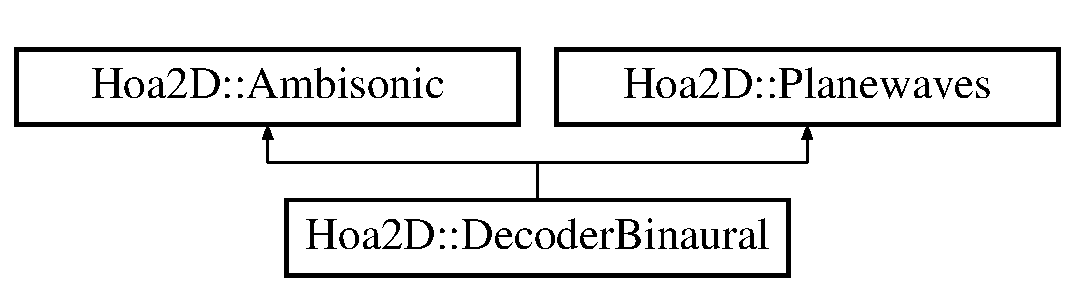
\includegraphics[height=2.000000cm]{class_hoa2_d_1_1_decoder_binaural}
\end{center}
\end{figure}
\subsection*{Public Member Functions}
\begin{DoxyCompactItemize}
\item 
\hyperlink{class_hoa2_d_1_1_decoder_binaural_a614b402069c035eb1bb03d3ec79c4098}{Decoder\-Binaural} (unsigned int order)
\begin{DoxyCompactList}\small\item\em The binaural decoder constructor. \end{DoxyCompactList}\item 
\hyperlink{class_hoa2_d_1_1_decoder_binaural_a3aa8b84a571c2c031dcae2b94b8737e4}{$\sim$\-Decoder\-Binaural} ()
\begin{DoxyCompactList}\small\item\em The binaural decoder destructor. \end{DoxyCompactList}\item 
bool \hyperlink{class_hoa2_d_1_1_decoder_binaural_a8cb958da4f7f5f5888cd894a52f69aa5}{get\-State} () const 
\begin{DoxyCompactList}\small\item\em Retrieve if the impulses has been loaded. \end{DoxyCompactList}\item 
std\-::string \hyperlink{class_hoa2_d_1_1_decoder_binaural_a045e4d443418211eca3074e10719ecd5}{get\-Channel\-Name} (unsigned int index)
\begin{DoxyCompactList}\small\item\em Retrieve a name for a channel. \end{DoxyCompactList}\item 
void \hyperlink{class_hoa2_d_1_1_decoder_binaural_accbfe84ed3e43f1e9ca93e58edb7020f}{process} (const float $\ast$const $\ast$inputs, float $\ast$$\ast$outputs)
\begin{DoxyCompactList}\small\item\em This method performs the binaural decoding with single precision. \end{DoxyCompactList}\item 
void \hyperlink{class_hoa2_d_1_1_decoder_binaural_afab13c873d9c9b1a883bcc993ec0ec35}{process} (const double $\ast$const $\ast$inputs, double $\ast$$\ast$outputs)
\begin{DoxyCompactList}\small\item\em This method performs the binaural decoding with double precision. \end{DoxyCompactList}\end{DoxyCompactItemize}
\subsection*{Additional Inherited Members}


\subsection{Detailed Description}
The ambisonic binaural decoder. 

The binaural decoder should be used to decode an ambisonic sound field for headphones. 

Definition at line 155 of file Decoder.\-h.



\subsection{Constructor \& Destructor Documentation}
\hypertarget{class_hoa2_d_1_1_decoder_binaural_a614b402069c035eb1bb03d3ec79c4098}{\index{Hoa2\-D\-::\-Decoder\-Binaural@{Hoa2\-D\-::\-Decoder\-Binaural}!Decoder\-Binaural@{Decoder\-Binaural}}
\index{Decoder\-Binaural@{Decoder\-Binaural}!Hoa2D::DecoderBinaural@{Hoa2\-D\-::\-Decoder\-Binaural}}
\subsubsection[{Decoder\-Binaural}]{\setlength{\rightskip}{0pt plus 5cm}Hoa2\-D\-::\-Decoder\-Binaural\-::\-Decoder\-Binaural (
\begin{DoxyParamCaption}
\item[{unsigned int}]{order}
\end{DoxyParamCaption}
)}}\label{class_hoa2_d_1_1_decoder_binaural_a614b402069c035eb1bb03d3ec79c4098}


The binaural decoder constructor. 

\begin{DoxyVerb}The binaural decoder constructor allocates and initialize the member values to the decoding matrix depending of a decomposition order and a number of channels. The order and the number of channels must be at least 1 and the maximum order is 35.
\end{DoxyVerb}



\begin{DoxyParams}{Parameters}
{\em order} & The order \\
\hline
{\em number\-Of\-Channels} & The number of channels. \\
\hline
\end{DoxyParams}


Definition at line 206 of file Decoder.\-cpp.

\hypertarget{class_hoa2_d_1_1_decoder_binaural_a3aa8b84a571c2c031dcae2b94b8737e4}{\index{Hoa2\-D\-::\-Decoder\-Binaural@{Hoa2\-D\-::\-Decoder\-Binaural}!$\sim$\-Decoder\-Binaural@{$\sim$\-Decoder\-Binaural}}
\index{$\sim$\-Decoder\-Binaural@{$\sim$\-Decoder\-Binaural}!Hoa2D::DecoderBinaural@{Hoa2\-D\-::\-Decoder\-Binaural}}
\subsubsection[{$\sim$\-Decoder\-Binaural}]{\setlength{\rightskip}{0pt plus 5cm}Hoa2\-D\-::\-Decoder\-Binaural\-::$\sim$\-Decoder\-Binaural (
\begin{DoxyParamCaption}
{}
\end{DoxyParamCaption}
)}}\label{class_hoa2_d_1_1_decoder_binaural_a3aa8b84a571c2c031dcae2b94b8737e4}


The binaural decoder destructor. 

The binaural decoder destructor free the memory. 

Definition at line 409 of file Decoder.\-cpp.



\subsection{Member Function Documentation}
\hypertarget{class_hoa2_d_1_1_decoder_binaural_a045e4d443418211eca3074e10719ecd5}{\index{Hoa2\-D\-::\-Decoder\-Binaural@{Hoa2\-D\-::\-Decoder\-Binaural}!get\-Channel\-Name@{get\-Channel\-Name}}
\index{get\-Channel\-Name@{get\-Channel\-Name}!Hoa2D::DecoderBinaural@{Hoa2\-D\-::\-Decoder\-Binaural}}
\subsubsection[{get\-Channel\-Name}]{\setlength{\rightskip}{0pt plus 5cm}std\-::string Hoa2\-D\-::\-Decoder\-Binaural\-::get\-Channel\-Name (
\begin{DoxyParamCaption}
\item[{unsigned int}]{index}
\end{DoxyParamCaption}
)\hspace{0.3cm}{\ttfamily [inline]}}}\label{class_hoa2_d_1_1_decoder_binaural_a045e4d443418211eca3074e10719ecd5}


Retrieve a name for a channel. 

Retrieve a name for a channel in a std\-::string format that will be \char`\"{}\-Headphone Left\char`\"{} or \char`\"{}\-Headphone Right\char`\"{}.


\begin{DoxyParams}{Parameters}
{\em index} & The index of a channel. \\
\hline
\end{DoxyParams}
\begin{DoxyReturn}{Returns}
The method returns a name for the channel that contains its index and its azimuth if the channel exists, otherwise the function generates an error. 
\end{DoxyReturn}


Definition at line 219 of file Decoder.\-h.

\hypertarget{class_hoa2_d_1_1_decoder_binaural_a8cb958da4f7f5f5888cd894a52f69aa5}{\index{Hoa2\-D\-::\-Decoder\-Binaural@{Hoa2\-D\-::\-Decoder\-Binaural}!get\-State@{get\-State}}
\index{get\-State@{get\-State}!Hoa2D::DecoderBinaural@{Hoa2\-D\-::\-Decoder\-Binaural}}
\subsubsection[{get\-State}]{\setlength{\rightskip}{0pt plus 5cm}bool Hoa2\-D\-::\-Decoder\-Binaural\-::get\-State (
\begin{DoxyParamCaption}
{}
\end{DoxyParamCaption}
) const\hspace{0.3cm}{\ttfamily [inline]}}}\label{class_hoa2_d_1_1_decoder_binaural_a8cb958da4f7f5f5888cd894a52f69aa5}


Retrieve if the impulses has been loaded. 

Retrieve if the impulses has been loaded.

\begin{DoxyReturn}{Returns}
The true if the impulses has been loaded and false if not. 
\end{DoxyReturn}


Definition at line 203 of file Decoder.\-h.

\hypertarget{class_hoa2_d_1_1_decoder_binaural_accbfe84ed3e43f1e9ca93e58edb7020f}{\index{Hoa2\-D\-::\-Decoder\-Binaural@{Hoa2\-D\-::\-Decoder\-Binaural}!process@{process}}
\index{process@{process}!Hoa2D::DecoderBinaural@{Hoa2\-D\-::\-Decoder\-Binaural}}
\subsubsection[{process}]{\setlength{\rightskip}{0pt plus 5cm}void Hoa2\-D\-::\-Decoder\-Binaural\-::process (
\begin{DoxyParamCaption}
\item[{const float $\ast$const $\ast$}]{inputs, }
\item[{float $\ast$$\ast$}]{outputs}
\end{DoxyParamCaption}
)}}\label{class_hoa2_d_1_1_decoder_binaural_accbfe84ed3e43f1e9ca93e58edb7020f}


This method performs the binaural decoding with single precision. 

\begin{DoxyVerb}You should use this method for in-place or not-in-place processing and performs the binaural decoding sample by sample. The inputs array contains the spherical harmonics samples and the minimum size must be the number of harmonics and the outputs array contains the headphones samples and the minimum size must be 2.
\end{DoxyVerb}



\begin{DoxyParams}{Parameters}
{\em inputs} & The input sample. \\
\hline
{\em outputs} & The output array that contains samples destinated to channels. \\
\hline
\end{DoxyParams}


Definition at line 340 of file Decoder.\-cpp.

\hypertarget{class_hoa2_d_1_1_decoder_binaural_afab13c873d9c9b1a883bcc993ec0ec35}{\index{Hoa2\-D\-::\-Decoder\-Binaural@{Hoa2\-D\-::\-Decoder\-Binaural}!process@{process}}
\index{process@{process}!Hoa2D::DecoderBinaural@{Hoa2\-D\-::\-Decoder\-Binaural}}
\subsubsection[{process}]{\setlength{\rightskip}{0pt plus 5cm}void Hoa2\-D\-::\-Decoder\-Binaural\-::process (
\begin{DoxyParamCaption}
\item[{const double $\ast$const $\ast$}]{inputs, }
\item[{double $\ast$$\ast$}]{outputs}
\end{DoxyParamCaption}
)}}\label{class_hoa2_d_1_1_decoder_binaural_afab13c873d9c9b1a883bcc993ec0ec35}


This method performs the binaural decoding with double precision. 

\begin{DoxyVerb}You should use this method for in-place or not-in-place processing and performs the binaural decoding sample by sample. The inputs array contains the spherical harmonics samples and the minimum size must be the number of harmonics and the outputs array contains the headphones samples and the minimum size must be 2.
\end{DoxyVerb}



\begin{DoxyParams}{Parameters}
{\em input} & The input sample. \\
\hline
{\em outputs} & The output array that contains samples destinated to channels. \\
\hline
\end{DoxyParams}


Definition at line 371 of file Decoder.\-cpp.



The documentation for this class was generated from the following files\-:\begin{DoxyCompactItemize}
\item 
/\-Users/\-Pierre/\-Source\-Tree/\-Hoa\-Library/\-Sources/\-Hoa2\-D/Decoder.\-h\item 
/\-Users/\-Pierre/\-Source\-Tree/\-Hoa\-Library/\-Sources/\-Hoa2\-D/Decoder.\-cpp\end{DoxyCompactItemize}

\hypertarget{class_hoa2_d_1_1_decoder_irregular}{\section{Hoa2\-D\-:\-:Decoder\-Irregular Class Reference}
\label{class_hoa2_d_1_1_decoder_irregular}\index{Hoa2\-D\-::\-Decoder\-Irregular@{Hoa2\-D\-::\-Decoder\-Irregular}}
}


The ambisonic irregular decoder.  




{\ttfamily \#include $<$Decoder.\-h$>$}

Inheritance diagram for Hoa2\-D\-:\-:Decoder\-Irregular\-:\begin{figure}[H]
\begin{center}
\leavevmode
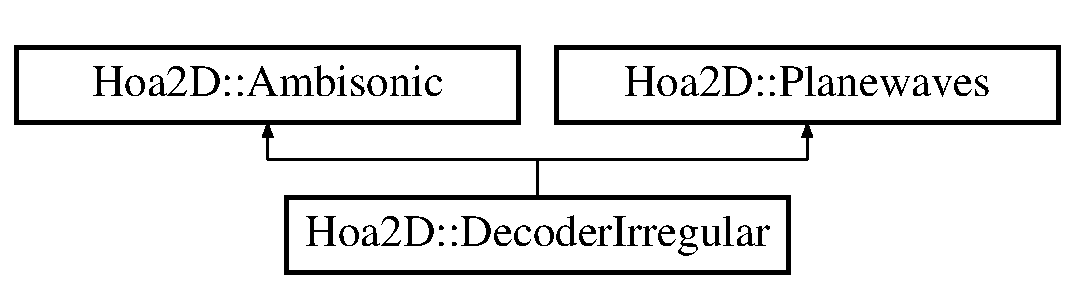
\includegraphics[height=2.000000cm]{class_hoa2_d_1_1_decoder_irregular}
\end{center}
\end{figure}
\subsection*{Public Member Functions}
\begin{DoxyCompactItemize}
\item 
\hyperlink{class_hoa2_d_1_1_decoder_irregular_a6847d61194817c336f323f21b757a67a}{Decoder\-Irregular} (unsigned int order, unsigned int number\-Of\-Channels)
\begin{DoxyCompactList}\small\item\em The irregular decoder constructor. \end{DoxyCompactList}\item 
\hyperlink{class_hoa2_d_1_1_decoder_irregular_af8a618d1d04c00f33c360fde6d09e03f}{$\sim$\-Decoder\-Irregular} ()
\begin{DoxyCompactList}\small\item\em The irregular decoder destructor. \end{DoxyCompactList}\item 
void \hyperlink{class_hoa2_d_1_1_decoder_irregular_ab74543528e37f6455de5452f00ac7c1c}{set\-Channel\-Position} (unsigned int index, double azimuth)
\begin{DoxyCompactList}\small\item\em Set the azimuth of a channel. \end{DoxyCompactList}\item 
void \hyperlink{class_hoa2_d_1_1_decoder_irregular_a6c4b42a6c7f9030b4db0d53186a9d6e0}{set\-Channels\-Position} (double $\ast$azimuths)
\begin{DoxyCompactList}\small\item\em Set the azimtuh of all the channels. \end{DoxyCompactList}\item 
void \hyperlink{class_hoa2_d_1_1_decoder_irregular_aacb9c2de89e276d0ede87e2ecfd2bde4}{process} (const float $\ast$input, float $\ast$output)
\begin{DoxyCompactList}\small\item\em This method performs the irregular decoding with single precision. \end{DoxyCompactList}\item 
void \hyperlink{class_hoa2_d_1_1_decoder_irregular_aa94b51fed5c341c0980d0d0ba9c53414}{process} (const double $\ast$input, double $\ast$output)
\begin{DoxyCompactList}\small\item\em This method performs the irregular decoding with double precision. \end{DoxyCompactList}\end{DoxyCompactItemize}
\subsection*{Additional Inherited Members}


\subsection{Detailed Description}
The ambisonic irregular decoder. 

The irregular decoder should be used to decode an ambisonic sound field for a set a channels not equally spaced on a circle, like stereo or 5.\-1, depending on a decomposition order. The number of channels must be at least 1. 

Definition at line 85 of file Decoder.\-h.



\subsection{Constructor \& Destructor Documentation}
\hypertarget{class_hoa2_d_1_1_decoder_irregular_a6847d61194817c336f323f21b757a67a}{\index{Hoa2\-D\-::\-Decoder\-Irregular@{Hoa2\-D\-::\-Decoder\-Irregular}!Decoder\-Irregular@{Decoder\-Irregular}}
\index{Decoder\-Irregular@{Decoder\-Irregular}!Hoa2D::DecoderIrregular@{Hoa2\-D\-::\-Decoder\-Irregular}}
\subsubsection[{Decoder\-Irregular}]{\setlength{\rightskip}{0pt plus 5cm}Hoa2\-D\-::\-Decoder\-Irregular\-::\-Decoder\-Irregular (
\begin{DoxyParamCaption}
\item[{unsigned int}]{order, }
\item[{unsigned int}]{number\-Of\-Channels}
\end{DoxyParamCaption}
)}}\label{class_hoa2_d_1_1_decoder_irregular_a6847d61194817c336f323f21b757a67a}


The irregular decoder constructor. 

The irregular decoder constructor allocates and initialize the member values to the decoding matrix depending of a decomposition order and a number of channels. The order and the number of channels must be at least 1.


\begin{DoxyParams}{Parameters}
{\em order} & The order \\
\hline
{\em number\-Of\-Channels} & The number of channels. \\
\hline
\end{DoxyParams}


Definition at line 62 of file Decoder.\-cpp.

\hypertarget{class_hoa2_d_1_1_decoder_irregular_af8a618d1d04c00f33c360fde6d09e03f}{\index{Hoa2\-D\-::\-Decoder\-Irregular@{Hoa2\-D\-::\-Decoder\-Irregular}!$\sim$\-Decoder\-Irregular@{$\sim$\-Decoder\-Irregular}}
\index{$\sim$\-Decoder\-Irregular@{$\sim$\-Decoder\-Irregular}!Hoa2D::DecoderIrregular@{Hoa2\-D\-::\-Decoder\-Irregular}}
\subsubsection[{$\sim$\-Decoder\-Irregular}]{\setlength{\rightskip}{0pt plus 5cm}Hoa2\-D\-::\-Decoder\-Irregular\-::$\sim$\-Decoder\-Irregular (
\begin{DoxyParamCaption}
{}
\end{DoxyParamCaption}
)}}\label{class_hoa2_d_1_1_decoder_irregular_af8a618d1d04c00f33c360fde6d09e03f}


The irregular decoder destructor. 

The irregular decoder destructor free the memory. 

Definition at line 196 of file Decoder.\-cpp.



\subsection{Member Function Documentation}
\hypertarget{class_hoa2_d_1_1_decoder_irregular_aacb9c2de89e276d0ede87e2ecfd2bde4}{\index{Hoa2\-D\-::\-Decoder\-Irregular@{Hoa2\-D\-::\-Decoder\-Irregular}!process@{process}}
\index{process@{process}!Hoa2D::DecoderIrregular@{Hoa2\-D\-::\-Decoder\-Irregular}}
\subsubsection[{process}]{\setlength{\rightskip}{0pt plus 5cm}void Hoa2\-D\-::\-Decoder\-Irregular\-::process (
\begin{DoxyParamCaption}
\item[{const float $\ast$}]{input, }
\item[{float $\ast$}]{output}
\end{DoxyParamCaption}
)}}\label{class_hoa2_d_1_1_decoder_irregular_aacb9c2de89e276d0ede87e2ecfd2bde4}


This method performs the irregular decoding with single precision. 

You should use this method for in-\/place or not-\/in-\/place processing and performs the irregular decoding sample by sample. The inputs array contains the spherical harmonics samples and the minimum size must be the number of harmonics and the outputs array contains the channels samples and the minimum size must be the number of channels.


\begin{DoxyParams}{Parameters}
{\em input} & The input sample. \\
\hline
{\em outputs} & The output array that contains samples destinated to channels. \\
\hline
\end{DoxyParams}


Definition at line 186 of file Decoder.\-cpp.

\hypertarget{class_hoa2_d_1_1_decoder_irregular_aa94b51fed5c341c0980d0d0ba9c53414}{\index{Hoa2\-D\-::\-Decoder\-Irregular@{Hoa2\-D\-::\-Decoder\-Irregular}!process@{process}}
\index{process@{process}!Hoa2D::DecoderIrregular@{Hoa2\-D\-::\-Decoder\-Irregular}}
\subsubsection[{process}]{\setlength{\rightskip}{0pt plus 5cm}void Hoa2\-D\-::\-Decoder\-Irregular\-::process (
\begin{DoxyParamCaption}
\item[{const double $\ast$}]{input, }
\item[{double $\ast$}]{output}
\end{DoxyParamCaption}
)}}\label{class_hoa2_d_1_1_decoder_irregular_aa94b51fed5c341c0980d0d0ba9c53414}


This method performs the irregular decoding with double precision. 

You should use this method for in-\/place or not-\/in-\/place processing and performs the irregular decoding sample by sample. The inputs array contains the spherical harmonics samples and the minimum size must be the number of harmonics and the outputs array contains the channels samples and the minimum size must be the number of channels.


\begin{DoxyParams}{Parameters}
{\em input} & The input sample. \\
\hline
{\em outputs} & The output array that contains samples destinated to channels. \\
\hline
\end{DoxyParams}


Definition at line 191 of file Decoder.\-cpp.

\hypertarget{class_hoa2_d_1_1_decoder_irregular_ab74543528e37f6455de5452f00ac7c1c}{\index{Hoa2\-D\-::\-Decoder\-Irregular@{Hoa2\-D\-::\-Decoder\-Irregular}!set\-Channel\-Position@{set\-Channel\-Position}}
\index{set\-Channel\-Position@{set\-Channel\-Position}!Hoa2D::DecoderIrregular@{Hoa2\-D\-::\-Decoder\-Irregular}}
\subsubsection[{set\-Channel\-Position}]{\setlength{\rightskip}{0pt plus 5cm}void Hoa2\-D\-::\-Decoder\-Irregular\-::set\-Channel\-Position (
\begin{DoxyParamCaption}
\item[{unsigned int}]{index, }
\item[{double}]{azimuth}
\end{DoxyParamCaption}
)}}\label{class_hoa2_d_1_1_decoder_irregular_ab74543528e37f6455de5452f00ac7c1c}


Set the azimuth of a channel. 

Set the azimuth of a channel. The azimuth is in radian between 0 and 2 Pi, O is the front of the soundfield and Pi is the back of the sound field. The maximum index must be the number of channel -\/ 1.


\begin{DoxyParams}{Parameters}
{\em index} & The index of the loudspeaker. \\
\hline
{\em azimuth} & The azimuth.\\
\hline
\end{DoxyParams}
\begin{DoxySeeAlso}{See Also}
\hyperlink{class_hoa2_d_1_1_decoder_irregular_a6c4b42a6c7f9030b4db0d53186a9d6e0}{set\-Channels\-Position} 
\end{DoxySeeAlso}


Definition at line 82 of file Decoder.\-cpp.

\hypertarget{class_hoa2_d_1_1_decoder_irregular_a6c4b42a6c7f9030b4db0d53186a9d6e0}{\index{Hoa2\-D\-::\-Decoder\-Irregular@{Hoa2\-D\-::\-Decoder\-Irregular}!set\-Channels\-Position@{set\-Channels\-Position}}
\index{set\-Channels\-Position@{set\-Channels\-Position}!Hoa2D::DecoderIrregular@{Hoa2\-D\-::\-Decoder\-Irregular}}
\subsubsection[{set\-Channels\-Position}]{\setlength{\rightskip}{0pt plus 5cm}void Hoa2\-D\-::\-Decoder\-Irregular\-::set\-Channels\-Position (
\begin{DoxyParamCaption}
\item[{double $\ast$}]{azimuths}
\end{DoxyParamCaption}
)}}\label{class_hoa2_d_1_1_decoder_irregular_a6c4b42a6c7f9030b4db0d53186a9d6e0}


Set the azimtuh of all the channels. 

Set the azimtuh of all the channels. It is more efficient to set all the channels azimuths at the same time because even if only one channel has changed, all the decoding matrix have to be recomputed. The azimuths are in radian between 0 and 2 Pi, O is the front of the soundfield and Pi is the back of the sound field. The azimtuhs array must have a minimum size of the number of channels.


\begin{DoxyParams}{Parameters}
{\em azimuths} & The azimuths array.\\
\hline
\end{DoxyParams}
\begin{DoxySeeAlso}{See Also}
\hyperlink{class_hoa2_d_1_1_decoder_irregular_ab74543528e37f6455de5452f00ac7c1c}{set\-Channel\-Position} 
\end{DoxySeeAlso}


Definition at line 73 of file Decoder.\-cpp.



The documentation for this class was generated from the following files\-:\begin{DoxyCompactItemize}
\item 
/\-Users/elioton/\-Documents/programmation/\-C\-I\-C\-M/source\-Tree/\-Hoa\-Library/\-Sources/\-Hoa2\-D/Decoder.\-h\item 
/\-Users/elioton/\-Documents/programmation/\-C\-I\-C\-M/source\-Tree/\-Hoa\-Library/\-Sources/\-Hoa2\-D/Decoder.\-cpp\end{DoxyCompactItemize}

\hypertarget{class_hoa2_d_1_1_decoder_multi}{\section{Hoa2\-D\-:\-:Decoder\-Multi Class Reference}
\label{class_hoa2_d_1_1_decoder_multi}\index{Hoa2\-D\-::\-Decoder\-Multi@{Hoa2\-D\-::\-Decoder\-Multi}}
}


The ambisonic multi-\/decoder.  




{\ttfamily \#include $<$Decoder.\-h$>$}

Inheritance diagram for Hoa2\-D\-:\-:Decoder\-Multi\-:\begin{figure}[H]
\begin{center}
\leavevmode
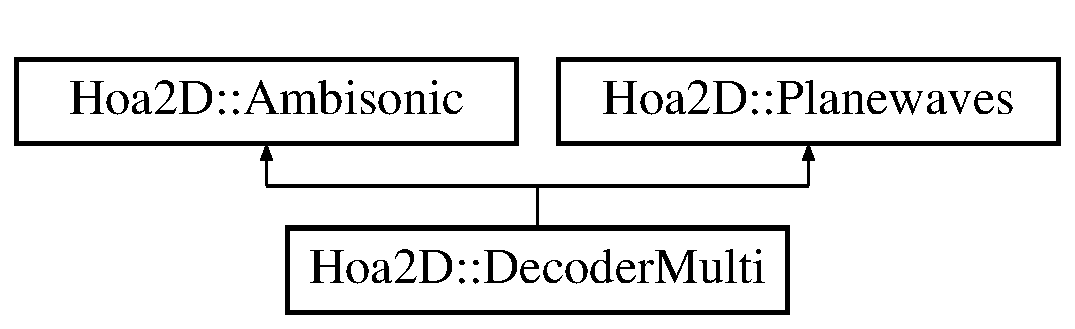
\includegraphics[height=2.000000cm]{class_hoa2_d_1_1_decoder_multi}
\end{center}
\end{figure}
\subsection*{Public Types}
\begin{DoxyCompactItemize}
\item 
enum \hyperlink{class_hoa2_d_1_1_decoder_multi_a0ac23d6bd77378d9cd5ddf6e71029300}{Mode} \{ \hyperlink{class_hoa2_d_1_1_decoder_multi_a0ac23d6bd77378d9cd5ddf6e71029300abaf1a2b64008b0199ced6e486911aed2}{Regular} = 0, 
\hyperlink{class_hoa2_d_1_1_decoder_multi_a0ac23d6bd77378d9cd5ddf6e71029300afad959e312fd3402f086633b221008a3}{Irregular} = 1, 
\hyperlink{class_hoa2_d_1_1_decoder_multi_a0ac23d6bd77378d9cd5ddf6e71029300a1d1ea5f4bbb54e7062cf1c74e8ae2db0}{Binaural} = 2
 \}
\end{DoxyCompactItemize}
\subsection*{Public Member Functions}
\begin{DoxyCompactItemize}
\item 
\hyperlink{class_hoa2_d_1_1_decoder_multi_afb4e1343b79a628a848b18a5237b4fe7}{Decoder\-Multi} (unsigned int order)
\begin{DoxyCompactList}\small\item\em The multi-\/decoder constructor. \end{DoxyCompactList}\item 
\hyperlink{class_hoa2_d_1_1_decoder_multi_a2a0aeff9157db4a486fa331b3dcd04cc}{$\sim$\-Decoder\-Multi} ()
\begin{DoxyCompactList}\small\item\em The multi-\/decoder destructor. \end{DoxyCompactList}\item 
void \hyperlink{class_hoa2_d_1_1_decoder_multi_a4c438ae79d50e9c01db919a76b506326}{set\-Decoding\-Mode} (\hyperlink{class_hoa2_d_1_1_decoder_multi_a0ac23d6bd77378d9cd5ddf6e71029300}{Mode} mode)
\begin{DoxyCompactList}\small\item\em Set the decoding mode. \end{DoxyCompactList}\item 
\hyperlink{class_hoa2_d_1_1_decoder_multi_a0ac23d6bd77378d9cd5ddf6e71029300}{Mode} \hyperlink{class_hoa2_d_1_1_decoder_multi_acc6e268ffd3e58bb9918d51c9dca282c}{get\-Decoding\-Mode} () const 
\begin{DoxyCompactList}\small\item\em Retrieve the decoding mode. \end{DoxyCompactList}\item 
void \hyperlink{class_hoa2_d_1_1_decoder_multi_a807edafa3240a9815a52d686307bb2b4}{set\-Number\-Of\-Channels} (unsigned int number\-Of\-Channels)
\begin{DoxyCompactList}\small\item\em Set the number of channels for the regular or irregular decoding. \end{DoxyCompactList}\item 
unsigned int \hyperlink{class_hoa2_d_1_1_decoder_multi_ae7c6a450a9a9ff184965f70556e7bf9d}{get\-Number\-Of\-Channels} () const 
\begin{DoxyCompactList}\small\item\em Retrieve the number of channels. \end{DoxyCompactList}\item 
void \hyperlink{class_hoa2_d_1_1_decoder_multi_a2cbf708c33f7bcb39895b058c1e139c1}{set\-Channels\-Offset} (double offset)
\begin{DoxyCompactList}\small\item\em Set the offset of the channels for the regular decoding. \end{DoxyCompactList}\item 
double \hyperlink{class_hoa2_d_1_1_decoder_multi_af31ea39af39be29e71f3b075470f16ad}{get\-Channels\-Offset} () const 
\begin{DoxyCompactList}\small\item\em Get the offset of the channels of the regular decoding. \end{DoxyCompactList}\item 
void \hyperlink{class_hoa2_d_1_1_decoder_multi_a42d2b7697ae84fd9ed43f8d1f4799dce}{set\-Channel\-Position} (unsigned int index, double azimuth)
\begin{DoxyCompactList}\small\item\em Set the azimuth of a channel for the irregular decoding mode. \end{DoxyCompactList}\item 
void \hyperlink{class_hoa2_d_1_1_decoder_multi_a226c24223ee381fd04dcbc44b4e8155e}{set\-Channels\-Position} (double $\ast$azimuths)
\begin{DoxyCompactList}\small\item\em Set the azimtuh of all the channels for the irregular decoding mode. \end{DoxyCompactList}\item 
void \hyperlink{class_hoa2_d_1_1_decoder_multi_aa15da12ba3889edc22ec9c148dd5c692}{set\-Sample\-Rate} (unsigned int sample\-Rate)
\begin{DoxyCompactList}\small\item\em Set the sample rate. \end{DoxyCompactList}\item 
void \hyperlink{class_hoa2_d_1_1_decoder_multi_a875eb671767c2f547453e6d7a1401f15}{set\-Vector\-Size} (unsigned int vector\-Size)
\begin{DoxyCompactList}\small\item\em Set the vector size. \end{DoxyCompactList}\item 
bool \hyperlink{class_hoa2_d_1_1_decoder_multi_a67e02e68e5ddaa18aa46e874ab5b6ad0}{get\-Binaural\-State} () const 
\begin{DoxyCompactList}\small\item\em Retrieve if the binaural decoder is ready to process. \end{DoxyCompactList}\item 
double \hyperlink{class_hoa2_d_1_1_decoder_multi_a27e9a7dfb9e88e22470849f6f32c7270}{get\-Channel\-Azimuth} (unsigned int index) const 
\begin{DoxyCompactList}\small\item\em Retrieve the azimuth of a channel. \end{DoxyCompactList}\item 
double \hyperlink{class_hoa2_d_1_1_decoder_multi_a31085fe8704942e389e9e5cd00d195bd}{get\-Channel\-Abscissa} (unsigned int index) const 
\begin{DoxyCompactList}\small\item\em Retrieve the abscissa of a channel. \end{DoxyCompactList}\item 
double \hyperlink{class_hoa2_d_1_1_decoder_multi_a4a0032053910595155cf5299c883385b}{get\-Channel\-Ordinate} (unsigned int index) const 
\begin{DoxyCompactList}\small\item\em Retrieve the ordinate of a channel. \end{DoxyCompactList}\item 
std\-::string \hyperlink{class_hoa2_d_1_1_decoder_multi_af2208568e5aff57ade0ba5a00656db32}{get\-Channel\-Name} (unsigned int index)
\begin{DoxyCompactList}\small\item\em Retrieve a name for a channel. \end{DoxyCompactList}\item 
void \hyperlink{class_hoa2_d_1_1_decoder_multi_a215385080edb593cb2d8c0e7124d0c00}{process\-Binaural} (const float $\ast$const $\ast$inputs, float $\ast$$\ast$outputs)
\begin{DoxyCompactList}\small\item\em This method performs the binaural decoding with single precision. \end{DoxyCompactList}\item 
void \hyperlink{class_hoa2_d_1_1_decoder_multi_ac2aed267552cfa2535156742529bfa54}{process\-Binaural} (const double $\ast$const $\ast$inputs, double $\ast$$\ast$outputs)
\begin{DoxyCompactList}\small\item\em This method performs the binaural decoding with double precision. \end{DoxyCompactList}\item 
void \hyperlink{class_hoa2_d_1_1_decoder_multi_a7d4d1130db9e008e178a4210571d9f97}{process\-Regular} (const float $\ast$inputs, float $\ast$outputs)
\begin{DoxyCompactList}\small\item\em This method performs the decoding depending of the mode with single precision. \end{DoxyCompactList}\item 
void \hyperlink{class_hoa2_d_1_1_decoder_multi_a594583b4853dcabf5f655412faad0fe7}{process\-Regular} (const double $\ast$inputs, double $\ast$outputs)
\begin{DoxyCompactList}\small\item\em This method performs the regular decoding with single precision. \end{DoxyCompactList}\item 
void \hyperlink{class_hoa2_d_1_1_decoder_multi_ae7b3be8b1b39a2242a4a270d5278a4f6}{process\-Irregular} (const float $\ast$inputs, float $\ast$outputs)
\begin{DoxyCompactList}\small\item\em This method performs the irregular decoding with single precision. \end{DoxyCompactList}\item 
void \hyperlink{class_hoa2_d_1_1_decoder_multi_a11493b383a19d621202acebb17568000}{process\-Irregular} (const double $\ast$inputs, double $\ast$outputs)
\begin{DoxyCompactList}\small\item\em This method performs the irregular decoding with single precision. \end{DoxyCompactList}\end{DoxyCompactItemize}
\subsection*{Additional Inherited Members}


\subsection{Detailed Description}
The ambisonic multi-\/decoder. 

The multi-\/decoder is a class that facilitates the use of the three decoder \-: regular, irregular and binaural. 

Definition at line 263 of file Decoder.\-h.



\subsection{Member Enumeration Documentation}
\hypertarget{class_hoa2_d_1_1_decoder_multi_a0ac23d6bd77378d9cd5ddf6e71029300}{\index{Hoa2\-D\-::\-Decoder\-Multi@{Hoa2\-D\-::\-Decoder\-Multi}!Mode@{Mode}}
\index{Mode@{Mode}!Hoa2D::DecoderMulti@{Hoa2\-D\-::\-Decoder\-Multi}}
\subsubsection[{Mode}]{\setlength{\rightskip}{0pt plus 5cm}enum {\bf Hoa2\-D\-::\-Decoder\-Multi\-::\-Mode}}}\label{class_hoa2_d_1_1_decoder_multi_a0ac23d6bd77378d9cd5ddf6e71029300}
\begin{Desc}
\item[Enumerator]\par
\begin{description}
\index{Regular@{Regular}!Hoa2\-D\-::\-Decoder\-Multi@{Hoa2\-D\-::\-Decoder\-Multi}}\index{Hoa2\-D\-::\-Decoder\-Multi@{Hoa2\-D\-::\-Decoder\-Multi}!Regular@{Regular}}\item[{\em 
\hypertarget{class_hoa2_d_1_1_decoder_multi_a0ac23d6bd77378d9cd5ddf6e71029300abaf1a2b64008b0199ced6e486911aed2}{Regular}\label{class_hoa2_d_1_1_decoder_multi_a0ac23d6bd77378d9cd5ddf6e71029300abaf1a2b64008b0199ced6e486911aed2}
}]Regular Decoding \index{Irregular@{Irregular}!Hoa2\-D\-::\-Decoder\-Multi@{Hoa2\-D\-::\-Decoder\-Multi}}\index{Hoa2\-D\-::\-Decoder\-Multi@{Hoa2\-D\-::\-Decoder\-Multi}!Irregular@{Irregular}}\item[{\em 
\hypertarget{class_hoa2_d_1_1_decoder_multi_a0ac23d6bd77378d9cd5ddf6e71029300afad959e312fd3402f086633b221008a3}{Irregular}\label{class_hoa2_d_1_1_decoder_multi_a0ac23d6bd77378d9cd5ddf6e71029300afad959e312fd3402f086633b221008a3}
}]Irregular Decoding \index{Binaural@{Binaural}!Hoa2\-D\-::\-Decoder\-Multi@{Hoa2\-D\-::\-Decoder\-Multi}}\index{Hoa2\-D\-::\-Decoder\-Multi@{Hoa2\-D\-::\-Decoder\-Multi}!Binaural@{Binaural}}\item[{\em 
\hypertarget{class_hoa2_d_1_1_decoder_multi_a0ac23d6bd77378d9cd5ddf6e71029300a1d1ea5f4bbb54e7062cf1c74e8ae2db0}{Binaural}\label{class_hoa2_d_1_1_decoder_multi_a0ac23d6bd77378d9cd5ddf6e71029300a1d1ea5f4bbb54e7062cf1c74e8ae2db0}
}]Binaural Decoding \end{description}
\end{Desc}


Definition at line 267 of file Decoder.\-h.



\subsection{Constructor \& Destructor Documentation}
\hypertarget{class_hoa2_d_1_1_decoder_multi_afb4e1343b79a628a848b18a5237b4fe7}{\index{Hoa2\-D\-::\-Decoder\-Multi@{Hoa2\-D\-::\-Decoder\-Multi}!Decoder\-Multi@{Decoder\-Multi}}
\index{Decoder\-Multi@{Decoder\-Multi}!Hoa2D::DecoderMulti@{Hoa2\-D\-::\-Decoder\-Multi}}
\subsubsection[{Decoder\-Multi}]{\setlength{\rightskip}{0pt plus 5cm}Hoa2\-D\-::\-Decoder\-Multi\-::\-Decoder\-Multi (
\begin{DoxyParamCaption}
\item[{unsigned int}]{order}
\end{DoxyParamCaption}
)}}\label{class_hoa2_d_1_1_decoder_multi_afb4e1343b79a628a848b18a5237b4fe7}


The multi-\/decoder constructor. 

The multi-\/decoder constructor allocates and initialize the three decoder. The default decoder will be the regular one with 2 $\ast$ order + 2 number of channels.


\begin{DoxyParams}{Parameters}
{\em order} & The order \\
\hline
\end{DoxyParams}


Definition at line 440 of file Decoder.\-cpp.

\hypertarget{class_hoa2_d_1_1_decoder_multi_a2a0aeff9157db4a486fa331b3dcd04cc}{\index{Hoa2\-D\-::\-Decoder\-Multi@{Hoa2\-D\-::\-Decoder\-Multi}!$\sim$\-Decoder\-Multi@{$\sim$\-Decoder\-Multi}}
\index{$\sim$\-Decoder\-Multi@{$\sim$\-Decoder\-Multi}!Hoa2D::DecoderMulti@{Hoa2\-D\-::\-Decoder\-Multi}}
\subsubsection[{$\sim$\-Decoder\-Multi}]{\setlength{\rightskip}{0pt plus 5cm}Hoa2\-D\-::\-Decoder\-Multi\-::$\sim$\-Decoder\-Multi (
\begin{DoxyParamCaption}
{}
\end{DoxyParamCaption}
)}}\label{class_hoa2_d_1_1_decoder_multi_a2a0aeff9157db4a486fa331b3dcd04cc}


The multi-\/decoder destructor. 

The multi-\/decoder destructor free the memory. 

Definition at line 530 of file Decoder.\-cpp.



\subsection{Member Function Documentation}
\hypertarget{class_hoa2_d_1_1_decoder_multi_a67e02e68e5ddaa18aa46e874ab5b6ad0}{\index{Hoa2\-D\-::\-Decoder\-Multi@{Hoa2\-D\-::\-Decoder\-Multi}!get\-Binaural\-State@{get\-Binaural\-State}}
\index{get\-Binaural\-State@{get\-Binaural\-State}!Hoa2D::DecoderMulti@{Hoa2\-D\-::\-Decoder\-Multi}}
\subsubsection[{get\-Binaural\-State}]{\setlength{\rightskip}{0pt plus 5cm}bool Hoa2\-D\-::\-Decoder\-Multi\-::get\-Binaural\-State (
\begin{DoxyParamCaption}
{}
\end{DoxyParamCaption}
) const\hspace{0.3cm}{\ttfamily [inline]}}}\label{class_hoa2_d_1_1_decoder_multi_a67e02e68e5ddaa18aa46e874ab5b6ad0}


Retrieve if the binaural decoder is ready to process. 

Retrieve if the impulses has been loaded and the matrix allocated.

\begin{DoxyReturn}{Returns}
The true if the binaural decoder is ready to process and false if not. 
\end{DoxyReturn}


Definition at line 399 of file Decoder.\-h.

\hypertarget{class_hoa2_d_1_1_decoder_multi_a31085fe8704942e389e9e5cd00d195bd}{\index{Hoa2\-D\-::\-Decoder\-Multi@{Hoa2\-D\-::\-Decoder\-Multi}!get\-Channel\-Abscissa@{get\-Channel\-Abscissa}}
\index{get\-Channel\-Abscissa@{get\-Channel\-Abscissa}!Hoa2D::DecoderMulti@{Hoa2\-D\-::\-Decoder\-Multi}}
\subsubsection[{get\-Channel\-Abscissa}]{\setlength{\rightskip}{0pt plus 5cm}double Hoa2\-D\-::\-Decoder\-Multi\-::get\-Channel\-Abscissa (
\begin{DoxyParamCaption}
\item[{unsigned int}]{index}
\end{DoxyParamCaption}
) const\hspace{0.3cm}{\ttfamily [inline]}}}\label{class_hoa2_d_1_1_decoder_multi_a31085fe8704942e389e9e5cd00d195bd}


Retrieve the abscissa of a channel. 

Retrieve the abscissa of a channel. The abscissa is between -\/1 and 1, -\/1 is the left of the soundfield, 0 is the center of the soundfield and 1 is the right of the soundfield. The maximum index must be the number of channels -\/ 1.


\begin{DoxyParams}{Parameters}
{\em index} & The index of the loudspeaker. \\
\hline
\end{DoxyParams}
\begin{DoxyReturn}{Returns}
The abscissa of the channel if the channel exists, otherwise the function generates an error.
\end{DoxyReturn}
\begin{DoxySeeAlso}{See Also}
\hyperlink{class_hoa2_d_1_1_decoder_multi_a27e9a7dfb9e88e22470849f6f32c7270}{get\-Channel\-Azimuth} 

\hyperlink{class_hoa2_d_1_1_decoder_multi_a4a0032053910595155cf5299c883385b}{get\-Channel\-Ordinate} 

\hyperlink{class_hoa2_d_1_1_decoder_multi_af2208568e5aff57ade0ba5a00656db32}{get\-Channel\-Name} 
\end{DoxySeeAlso}


Definition at line 438 of file Decoder.\-h.

\hypertarget{class_hoa2_d_1_1_decoder_multi_a27e9a7dfb9e88e22470849f6f32c7270}{\index{Hoa2\-D\-::\-Decoder\-Multi@{Hoa2\-D\-::\-Decoder\-Multi}!get\-Channel\-Azimuth@{get\-Channel\-Azimuth}}
\index{get\-Channel\-Azimuth@{get\-Channel\-Azimuth}!Hoa2D::DecoderMulti@{Hoa2\-D\-::\-Decoder\-Multi}}
\subsubsection[{get\-Channel\-Azimuth}]{\setlength{\rightskip}{0pt plus 5cm}double Hoa2\-D\-::\-Decoder\-Multi\-::get\-Channel\-Azimuth (
\begin{DoxyParamCaption}
\item[{unsigned int}]{index}
\end{DoxyParamCaption}
) const\hspace{0.3cm}{\ttfamily [inline]}}}\label{class_hoa2_d_1_1_decoder_multi_a27e9a7dfb9e88e22470849f6f32c7270}


Retrieve the azimuth of a channel. 

Retrieve the azimuth of a channel. The azimuth of the channel is in radian, 0 radian is at the front of the soundfield and Pi is at the back of the sound field. The maximum index must be the number of channels -\/ 1.


\begin{DoxyParams}{Parameters}
{\em index} & The index of the channel. \\
\hline
\end{DoxyParams}
\begin{DoxyReturn}{Returns}
The azimuth of the channel if the channel exists, otherwise the function generates an error.
\end{DoxyReturn}
\begin{DoxySeeAlso}{See Also}
\hyperlink{class_hoa2_d_1_1_decoder_multi_a31085fe8704942e389e9e5cd00d195bd}{get\-Channel\-Abscissa} 

\hyperlink{class_hoa2_d_1_1_decoder_multi_a4a0032053910595155cf5299c883385b}{get\-Channel\-Ordinate} 

\hyperlink{class_hoa2_d_1_1_decoder_multi_af2208568e5aff57ade0ba5a00656db32}{get\-Channel\-Name} 
\end{DoxySeeAlso}


Definition at line 417 of file Decoder.\-h.

\hypertarget{class_hoa2_d_1_1_decoder_multi_af2208568e5aff57ade0ba5a00656db32}{\index{Hoa2\-D\-::\-Decoder\-Multi@{Hoa2\-D\-::\-Decoder\-Multi}!get\-Channel\-Name@{get\-Channel\-Name}}
\index{get\-Channel\-Name@{get\-Channel\-Name}!Hoa2D::DecoderMulti@{Hoa2\-D\-::\-Decoder\-Multi}}
\subsubsection[{get\-Channel\-Name}]{\setlength{\rightskip}{0pt plus 5cm}std\-::string Hoa2\-D\-::\-Decoder\-Multi\-::get\-Channel\-Name (
\begin{DoxyParamCaption}
\item[{unsigned int}]{index}
\end{DoxyParamCaption}
)\hspace{0.3cm}{\ttfamily [inline]}}}\label{class_hoa2_d_1_1_decoder_multi_af2208568e5aff57ade0ba5a00656db32}


Retrieve a name for a channel. 

Retrieve a name for a channel in a std\-::string format, look at each decoder for further informations.


\begin{DoxyParams}{Parameters}
{\em index} & The index of a channel. \\
\hline
\end{DoxyParams}
\begin{DoxyReturn}{Returns}
The method returns a name for the channel. 
\end{DoxyReturn}


Definition at line 475 of file Decoder.\-h.

\hypertarget{class_hoa2_d_1_1_decoder_multi_a4a0032053910595155cf5299c883385b}{\index{Hoa2\-D\-::\-Decoder\-Multi@{Hoa2\-D\-::\-Decoder\-Multi}!get\-Channel\-Ordinate@{get\-Channel\-Ordinate}}
\index{get\-Channel\-Ordinate@{get\-Channel\-Ordinate}!Hoa2D::DecoderMulti@{Hoa2\-D\-::\-Decoder\-Multi}}
\subsubsection[{get\-Channel\-Ordinate}]{\setlength{\rightskip}{0pt plus 5cm}double Hoa2\-D\-::\-Decoder\-Multi\-::get\-Channel\-Ordinate (
\begin{DoxyParamCaption}
\item[{unsigned int}]{index}
\end{DoxyParamCaption}
) const\hspace{0.3cm}{\ttfamily [inline]}}}\label{class_hoa2_d_1_1_decoder_multi_a4a0032053910595155cf5299c883385b}


Retrieve the ordinate of a channel. 

Retrieve the ordinate of a channel. The ordinate is between -\/1 and 1, -\/1 is the back of the soundfield, 0 is the center of the soundfield and 1 is the front of the soundfield. The maximum index must be the number of channels -\/ 1.


\begin{DoxyParams}{Parameters}
{\em index} & The index of the channel. \\
\hline
\end{DoxyParams}
\begin{DoxyReturn}{Returns}
The ordinate of the channel if the channel exists, otherwise the function generates an error.
\end{DoxyReturn}
\begin{DoxySeeAlso}{See Also}
\hyperlink{class_hoa2_d_1_1_decoder_multi_a27e9a7dfb9e88e22470849f6f32c7270}{get\-Channel\-Azimuth} 

\hyperlink{class_hoa2_d_1_1_decoder_multi_a31085fe8704942e389e9e5cd00d195bd}{get\-Channel\-Abscissa} 

\hyperlink{class_hoa2_d_1_1_decoder_multi_af2208568e5aff57ade0ba5a00656db32}{get\-Channel\-Name} 
\end{DoxySeeAlso}


Definition at line 458 of file Decoder.\-h.

\hypertarget{class_hoa2_d_1_1_decoder_multi_af31ea39af39be29e71f3b075470f16ad}{\index{Hoa2\-D\-::\-Decoder\-Multi@{Hoa2\-D\-::\-Decoder\-Multi}!get\-Channels\-Offset@{get\-Channels\-Offset}}
\index{get\-Channels\-Offset@{get\-Channels\-Offset}!Hoa2D::DecoderMulti@{Hoa2\-D\-::\-Decoder\-Multi}}
\subsubsection[{get\-Channels\-Offset}]{\setlength{\rightskip}{0pt plus 5cm}double Hoa2\-D\-::\-Decoder\-Multi\-::get\-Channels\-Offset (
\begin{DoxyParamCaption}
{}
\end{DoxyParamCaption}
) const\hspace{0.3cm}{\ttfamily [inline]}}}\label{class_hoa2_d_1_1_decoder_multi_af31ea39af39be29e71f3b075470f16ad}


Get the offset of the channels of the regular decoding. 

Retreive the azimuth offset of the channels in radian the regular decoding.

\begin{DoxyReturn}{Returns}
The offset of the channels if the regular decoding mode is active, otherwise it returns 0. 
\end{DoxyReturn}


Definition at line 348 of file Decoder.\-h.

\hypertarget{class_hoa2_d_1_1_decoder_multi_acc6e268ffd3e58bb9918d51c9dca282c}{\index{Hoa2\-D\-::\-Decoder\-Multi@{Hoa2\-D\-::\-Decoder\-Multi}!get\-Decoding\-Mode@{get\-Decoding\-Mode}}
\index{get\-Decoding\-Mode@{get\-Decoding\-Mode}!Hoa2D::DecoderMulti@{Hoa2\-D\-::\-Decoder\-Multi}}
\subsubsection[{get\-Decoding\-Mode}]{\setlength{\rightskip}{0pt plus 5cm}{\bf Mode} Hoa2\-D\-::\-Decoder\-Multi\-::get\-Decoding\-Mode (
\begin{DoxyParamCaption}
{}
\end{DoxyParamCaption}
) const\hspace{0.3cm}{\ttfamily [inline]}}}\label{class_hoa2_d_1_1_decoder_multi_acc6e268ffd3e58bb9918d51c9dca282c}


Retrieve the decoding mode. 

Retrieve the current decoding mode of the multi-\/decoder.

\begin{DoxyReturn}{Returns}
The decoding mode; 
\end{DoxyReturn}


Definition at line 309 of file Decoder.\-h.

\hypertarget{class_hoa2_d_1_1_decoder_multi_ae7c6a450a9a9ff184965f70556e7bf9d}{\index{Hoa2\-D\-::\-Decoder\-Multi@{Hoa2\-D\-::\-Decoder\-Multi}!get\-Number\-Of\-Channels@{get\-Number\-Of\-Channels}}
\index{get\-Number\-Of\-Channels@{get\-Number\-Of\-Channels}!Hoa2D::DecoderMulti@{Hoa2\-D\-::\-Decoder\-Multi}}
\subsubsection[{get\-Number\-Of\-Channels}]{\setlength{\rightskip}{0pt plus 5cm}unsigned int Hoa2\-D\-::\-Decoder\-Multi\-::get\-Number\-Of\-Channels (
\begin{DoxyParamCaption}
{}
\end{DoxyParamCaption}
) const\hspace{0.3cm}{\ttfamily [inline]}}}\label{class_hoa2_d_1_1_decoder_multi_ae7c6a450a9a9ff184965f70556e7bf9d}


Retrieve the number of channels. 

Retrieve the number of channels of the planewave class.

\begin{DoxyReturn}{Returns}
The number of channels. 
\end{DoxyReturn}


Definition at line 326 of file Decoder.\-h.

\hypertarget{class_hoa2_d_1_1_decoder_multi_a215385080edb593cb2d8c0e7124d0c00}{\index{Hoa2\-D\-::\-Decoder\-Multi@{Hoa2\-D\-::\-Decoder\-Multi}!process\-Binaural@{process\-Binaural}}
\index{process\-Binaural@{process\-Binaural}!Hoa2D::DecoderMulti@{Hoa2\-D\-::\-Decoder\-Multi}}
\subsubsection[{process\-Binaural}]{\setlength{\rightskip}{0pt plus 5cm}void Hoa2\-D\-::\-Decoder\-Multi\-::process\-Binaural (
\begin{DoxyParamCaption}
\item[{const float $\ast$const $\ast$}]{inputs, }
\item[{float $\ast$$\ast$}]{outputs}
\end{DoxyParamCaption}
)\hspace{0.3cm}{\ttfamily [inline]}}}\label{class_hoa2_d_1_1_decoder_multi_a215385080edb593cb2d8c0e7124d0c00}


This method performs the binaural decoding with single precision. 

You should use this method for not-\/in-\/place processing and performs the binaural decoding on block of samples. The inputs matrix contains the spherical harmonics samples \-: inputs\mbox{[}number of harmonics\mbox{]}\mbox{[}vector size\mbox{]} and the outputs array contains the headphones samples \-: outputs\mbox{[}2\mbox{]}\mbox{[}vector size\mbox{]}.


\begin{DoxyParams}{Parameters}
{\em inputs} & The input samples. \\
\hline
{\em outputs} & The output array that contains samples destinated to channels. \\
\hline
\end{DoxyParams}


Definition at line 491 of file Decoder.\-h.

\hypertarget{class_hoa2_d_1_1_decoder_multi_ac2aed267552cfa2535156742529bfa54}{\index{Hoa2\-D\-::\-Decoder\-Multi@{Hoa2\-D\-::\-Decoder\-Multi}!process\-Binaural@{process\-Binaural}}
\index{process\-Binaural@{process\-Binaural}!Hoa2D::DecoderMulti@{Hoa2\-D\-::\-Decoder\-Multi}}
\subsubsection[{process\-Binaural}]{\setlength{\rightskip}{0pt plus 5cm}void Hoa2\-D\-::\-Decoder\-Multi\-::process\-Binaural (
\begin{DoxyParamCaption}
\item[{const double $\ast$const $\ast$}]{inputs, }
\item[{double $\ast$$\ast$}]{outputs}
\end{DoxyParamCaption}
)\hspace{0.3cm}{\ttfamily [inline]}}}\label{class_hoa2_d_1_1_decoder_multi_ac2aed267552cfa2535156742529bfa54}


This method performs the binaural decoding with double precision. 

You should use this method for not-\/in-\/place processing and performs the binaural decoding on block of samples. The inputs matrix contains the spherical harmonics samples \-: inputs\mbox{[}number of harmonics\mbox{]}\mbox{[}vector size\mbox{]} and the outputs array contains the headphones samples \-: outputs\mbox{[}2\mbox{]}\mbox{[}vector size\mbox{]}.


\begin{DoxyParams}{Parameters}
{\em inputs} & The input samples. \\
\hline
{\em outputs} & The output array that contains samples destinated to channels. \\
\hline
\end{DoxyParams}


Definition at line 502 of file Decoder.\-h.

\hypertarget{class_hoa2_d_1_1_decoder_multi_ae7b3be8b1b39a2242a4a270d5278a4f6}{\index{Hoa2\-D\-::\-Decoder\-Multi@{Hoa2\-D\-::\-Decoder\-Multi}!process\-Irregular@{process\-Irregular}}
\index{process\-Irregular@{process\-Irregular}!Hoa2D::DecoderMulti@{Hoa2\-D\-::\-Decoder\-Multi}}
\subsubsection[{process\-Irregular}]{\setlength{\rightskip}{0pt plus 5cm}void Hoa2\-D\-::\-Decoder\-Multi\-::process\-Irregular (
\begin{DoxyParamCaption}
\item[{const float $\ast$}]{inputs, }
\item[{float $\ast$}]{outputs}
\end{DoxyParamCaption}
)\hspace{0.3cm}{\ttfamily [inline]}}}\label{class_hoa2_d_1_1_decoder_multi_ae7b3be8b1b39a2242a4a270d5278a4f6}


This method performs the irregular decoding with single precision. 

You should use this method for in-\/place or not-\/in-\/place processing and performs the irregular decoding sample by sample. The inputs array contains the spherical harmonics samples and the minimum size must be the number of harmonics and the outputs array contains the channels samples and the minimum size must be the number of channels.


\begin{DoxyParams}{Parameters}
{\em input} & The input sample. \\
\hline
{\em outputs} & The output array that contains samples destinated to channels. \\
\hline
\end{DoxyParams}


Definition at line 535 of file Decoder.\-h.

\hypertarget{class_hoa2_d_1_1_decoder_multi_a11493b383a19d621202acebb17568000}{\index{Hoa2\-D\-::\-Decoder\-Multi@{Hoa2\-D\-::\-Decoder\-Multi}!process\-Irregular@{process\-Irregular}}
\index{process\-Irregular@{process\-Irregular}!Hoa2D::DecoderMulti@{Hoa2\-D\-::\-Decoder\-Multi}}
\subsubsection[{process\-Irregular}]{\setlength{\rightskip}{0pt plus 5cm}void Hoa2\-D\-::\-Decoder\-Multi\-::process\-Irregular (
\begin{DoxyParamCaption}
\item[{const double $\ast$}]{inputs, }
\item[{double $\ast$}]{outputs}
\end{DoxyParamCaption}
)\hspace{0.3cm}{\ttfamily [inline]}}}\label{class_hoa2_d_1_1_decoder_multi_a11493b383a19d621202acebb17568000}


This method performs the irregular decoding with single precision. 

You should use this method for in-\/place or not-\/in-\/place processing and performs the irregular decoding sample by sample. The inputs array contains the spherical harmonics samples and the minimum size must be the number of harmonics and the outputs array contains the channels samples and the minimum size must be the number of channels.


\begin{DoxyParams}{Parameters}
{\em input} & The input sample. \\
\hline
{\em outputs} & The output array that contains samples destinated to channels. \\
\hline
\end{DoxyParams}


Definition at line 546 of file Decoder.\-h.

\hypertarget{class_hoa2_d_1_1_decoder_multi_a7d4d1130db9e008e178a4210571d9f97}{\index{Hoa2\-D\-::\-Decoder\-Multi@{Hoa2\-D\-::\-Decoder\-Multi}!process\-Regular@{process\-Regular}}
\index{process\-Regular@{process\-Regular}!Hoa2D::DecoderMulti@{Hoa2\-D\-::\-Decoder\-Multi}}
\subsubsection[{process\-Regular}]{\setlength{\rightskip}{0pt plus 5cm}void Hoa2\-D\-::\-Decoder\-Multi\-::process\-Regular (
\begin{DoxyParamCaption}
\item[{const float $\ast$}]{inputs, }
\item[{float $\ast$}]{outputs}
\end{DoxyParamCaption}
)\hspace{0.3cm}{\ttfamily [inline]}}}\label{class_hoa2_d_1_1_decoder_multi_a7d4d1130db9e008e178a4210571d9f97}


This method performs the decoding depending of the mode with single precision. 

You should use this method for not-\/in-\/place processing and performs the binaural decoding on block of samples. The inputs matrix contains the spherical harmonics samples \-: inputs\mbox{[}number of harmonics\mbox{]}\mbox{[}vector size\mbox{]} and the outputs array contains the headphones samples \-: outputs\mbox{[}2\mbox{]}\mbox{[}vector size\mbox{]}.


\begin{DoxyParams}{Parameters}
{\em inputs} & The input samples. \\
\hline
{\em outputs} & The output array that contains samples destinated to channels. \\
\hline
\end{DoxyParams}


Definition at line 513 of file Decoder.\-h.

\hypertarget{class_hoa2_d_1_1_decoder_multi_a594583b4853dcabf5f655412faad0fe7}{\index{Hoa2\-D\-::\-Decoder\-Multi@{Hoa2\-D\-::\-Decoder\-Multi}!process\-Regular@{process\-Regular}}
\index{process\-Regular@{process\-Regular}!Hoa2D::DecoderMulti@{Hoa2\-D\-::\-Decoder\-Multi}}
\subsubsection[{process\-Regular}]{\setlength{\rightskip}{0pt plus 5cm}void Hoa2\-D\-::\-Decoder\-Multi\-::process\-Regular (
\begin{DoxyParamCaption}
\item[{const double $\ast$}]{inputs, }
\item[{double $\ast$}]{outputs}
\end{DoxyParamCaption}
)\hspace{0.3cm}{\ttfamily [inline]}}}\label{class_hoa2_d_1_1_decoder_multi_a594583b4853dcabf5f655412faad0fe7}


This method performs the regular decoding with single precision. 

You should use this method for in-\/place or not-\/in-\/place processing and performs the regular decoding sample by sample. The inputs array contains the spherical harmonics samples and the minimum size must be the number of harmonics and the outputs array contains the channels samples and the minimym size must be the number of channels.


\begin{DoxyParams}{Parameters}
{\em input} & The input sample. \\
\hline
{\em outputs} & The output array that contains samples destinated to channels. \\
\hline
\end{DoxyParams}


Definition at line 524 of file Decoder.\-h.

\hypertarget{class_hoa2_d_1_1_decoder_multi_a42d2b7697ae84fd9ed43f8d1f4799dce}{\index{Hoa2\-D\-::\-Decoder\-Multi@{Hoa2\-D\-::\-Decoder\-Multi}!set\-Channel\-Position@{set\-Channel\-Position}}
\index{set\-Channel\-Position@{set\-Channel\-Position}!Hoa2D::DecoderMulti@{Hoa2\-D\-::\-Decoder\-Multi}}
\subsubsection[{set\-Channel\-Position}]{\setlength{\rightskip}{0pt plus 5cm}void Hoa2\-D\-::\-Decoder\-Multi\-::set\-Channel\-Position (
\begin{DoxyParamCaption}
\item[{unsigned int}]{index, }
\item[{double}]{azimuth}
\end{DoxyParamCaption}
)}}\label{class_hoa2_d_1_1_decoder_multi_a42d2b7697ae84fd9ed43f8d1f4799dce}


Set the azimuth of a channel for the irregular decoding mode. 

Set the azimuth of a channel for the irregular decoding mode. The azimuth is in radian between 0 and 2 Pi, O is the front of the soundfield and Pi is the back of the sound field. The maximum index must be the number of channel -\/ 1.


\begin{DoxyParams}{Parameters}
{\em index} & The index of the loudspeaker. \\
\hline
{\em azimuth} & The azimuth.\\
\hline
\end{DoxyParams}
\begin{DoxySeeAlso}{See Also}
\hyperlink{class_hoa2_d_1_1_decoder_multi_a226c24223ee381fd04dcbc44b4e8155e}{set\-Channels\-Position} 
\end{DoxySeeAlso}


Definition at line 496 of file Decoder.\-cpp.

\hypertarget{class_hoa2_d_1_1_decoder_multi_a2cbf708c33f7bcb39895b058c1e139c1}{\index{Hoa2\-D\-::\-Decoder\-Multi@{Hoa2\-D\-::\-Decoder\-Multi}!set\-Channels\-Offset@{set\-Channels\-Offset}}
\index{set\-Channels\-Offset@{set\-Channels\-Offset}!Hoa2D::DecoderMulti@{Hoa2\-D\-::\-Decoder\-Multi}}
\subsubsection[{set\-Channels\-Offset}]{\setlength{\rightskip}{0pt plus 5cm}void Hoa2\-D\-::\-Decoder\-Multi\-::set\-Channels\-Offset (
\begin{DoxyParamCaption}
\item[{double}]{offset}
\end{DoxyParamCaption}
)}}\label{class_hoa2_d_1_1_decoder_multi_a2cbf708c33f7bcb39895b058c1e139c1}


Set the offset of the channels for the regular decoding. 

Set the azimuth offset of the channels in radian for the regular decoding, if the decoding mode.


\begin{DoxyParams}{Parameters}
{\em offset} & An azimuth value. \\
\hline
\end{DoxyParams}


Definition at line 488 of file Decoder.\-cpp.

\hypertarget{class_hoa2_d_1_1_decoder_multi_a226c24223ee381fd04dcbc44b4e8155e}{\index{Hoa2\-D\-::\-Decoder\-Multi@{Hoa2\-D\-::\-Decoder\-Multi}!set\-Channels\-Position@{set\-Channels\-Position}}
\index{set\-Channels\-Position@{set\-Channels\-Position}!Hoa2D::DecoderMulti@{Hoa2\-D\-::\-Decoder\-Multi}}
\subsubsection[{set\-Channels\-Position}]{\setlength{\rightskip}{0pt plus 5cm}void Hoa2\-D\-::\-Decoder\-Multi\-::set\-Channels\-Position (
\begin{DoxyParamCaption}
\item[{double $\ast$}]{azimuths}
\end{DoxyParamCaption}
)}}\label{class_hoa2_d_1_1_decoder_multi_a226c24223ee381fd04dcbc44b4e8155e}


Set the azimtuh of all the channels for the irregular decoding mode. 

Set the azimtuh of all the channels for the irregular decoding mode. It is more efficient to set all the channels azimuths at the same time because even if only one channel has changed, all the decoding matrix have to be recomputed. The azimuths are in radian between 0 and 2 Pi, O is the front of the soundfield and Pi is the back of the sound field. The azimtuhs array must have a minimum size of the number of channels.


\begin{DoxyParams}{Parameters}
{\em azimuths} & The azimuths array.\\
\hline
\end{DoxyParams}
\begin{DoxySeeAlso}{See Also}
\hyperlink{class_hoa2_d_1_1_decoder_multi_a42d2b7697ae84fd9ed43f8d1f4799dce}{set\-Channel\-Position} 
\end{DoxySeeAlso}


Definition at line 504 of file Decoder.\-cpp.

\hypertarget{class_hoa2_d_1_1_decoder_multi_a4c438ae79d50e9c01db919a76b506326}{\index{Hoa2\-D\-::\-Decoder\-Multi@{Hoa2\-D\-::\-Decoder\-Multi}!set\-Decoding\-Mode@{set\-Decoding\-Mode}}
\index{set\-Decoding\-Mode@{set\-Decoding\-Mode}!Hoa2D::DecoderMulti@{Hoa2\-D\-::\-Decoder\-Multi}}
\subsubsection[{set\-Decoding\-Mode}]{\setlength{\rightskip}{0pt plus 5cm}void Hoa2\-D\-::\-Decoder\-Multi\-::set\-Decoding\-Mode (
\begin{DoxyParamCaption}
\item[{{\bf Mode}}]{mode}
\end{DoxyParamCaption}
)}}\label{class_hoa2_d_1_1_decoder_multi_a4c438ae79d50e9c01db919a76b506326}


Set the decoding mode. 

Set the decoding mode. It will allocate the right decoder and initialize the class.


\begin{DoxyParams}{Parameters}
{\em mode} & The decoding mode. \\
\hline
\end{DoxyParams}


Definition at line 446 of file Decoder.\-cpp.

\hypertarget{class_hoa2_d_1_1_decoder_multi_a807edafa3240a9815a52d686307bb2b4}{\index{Hoa2\-D\-::\-Decoder\-Multi@{Hoa2\-D\-::\-Decoder\-Multi}!set\-Number\-Of\-Channels@{set\-Number\-Of\-Channels}}
\index{set\-Number\-Of\-Channels@{set\-Number\-Of\-Channels}!Hoa2D::DecoderMulti@{Hoa2\-D\-::\-Decoder\-Multi}}
\subsubsection[{set\-Number\-Of\-Channels}]{\setlength{\rightskip}{0pt plus 5cm}void Hoa2\-D\-::\-Decoder\-Multi\-::set\-Number\-Of\-Channels (
\begin{DoxyParamCaption}
\item[{unsigned int}]{number\-Of\-Channels}
\end{DoxyParamCaption}
)}}\label{class_hoa2_d_1_1_decoder_multi_a807edafa3240a9815a52d686307bb2b4}


Set the number of channels for the regular or irregular decoding. 

Set the number of channels for the regular or irregular decoding.


\begin{DoxyParams}{Parameters}
{\em number\-Of\-Channels} & The number of channels. \\
\hline
\end{DoxyParams}


Definition at line 471 of file Decoder.\-cpp.

\hypertarget{class_hoa2_d_1_1_decoder_multi_aa15da12ba3889edc22ec9c148dd5c692}{\index{Hoa2\-D\-::\-Decoder\-Multi@{Hoa2\-D\-::\-Decoder\-Multi}!set\-Sample\-Rate@{set\-Sample\-Rate}}
\index{set\-Sample\-Rate@{set\-Sample\-Rate}!Hoa2D::DecoderMulti@{Hoa2\-D\-::\-Decoder\-Multi}}
\subsubsection[{set\-Sample\-Rate}]{\setlength{\rightskip}{0pt plus 5cm}void Hoa2\-D\-::\-Decoder\-Multi\-::set\-Sample\-Rate (
\begin{DoxyParamCaption}
\item[{unsigned int}]{sample\-Rate}
\end{DoxyParamCaption}
)}}\label{class_hoa2_d_1_1_decoder_multi_aa15da12ba3889edc22ec9c148dd5c692}


Set the sample rate. 

Set the sample rate. The sample will change the impulse responses size and their sizes increase with it. The valid sample rate are 44100, 48000, 88200 and 9600. Setting the sample rate will load the impulse responses, it is essential to define it before the digital signal processing.


\begin{DoxyParams}{Parameters}
{\em sample\-Rate} & The sample rate.\\
\hline
\end{DoxyParams}
\begin{DoxySeeAlso}{See Also}
\hyperlink{class_hoa2_d_1_1_decoder_multi_a875eb671767c2f547453e6d7a1401f15}{set\-Vector\-Size} 
\end{DoxySeeAlso}


Definition at line 512 of file Decoder.\-cpp.

\hypertarget{class_hoa2_d_1_1_decoder_multi_a875eb671767c2f547453e6d7a1401f15}{\index{Hoa2\-D\-::\-Decoder\-Multi@{Hoa2\-D\-::\-Decoder\-Multi}!set\-Vector\-Size@{set\-Vector\-Size}}
\index{set\-Vector\-Size@{set\-Vector\-Size}!Hoa2D::DecoderMulti@{Hoa2\-D\-::\-Decoder\-Multi}}
\subsubsection[{set\-Vector\-Size}]{\setlength{\rightskip}{0pt plus 5cm}void Hoa2\-D\-::\-Decoder\-Multi\-::set\-Vector\-Size (
\begin{DoxyParamCaption}
\item[{unsigned int}]{vector\-Size}
\end{DoxyParamCaption}
)}}\label{class_hoa2_d_1_1_decoder_multi_a875eb671767c2f547453e6d7a1401f15}


Set the vector size. 

Set the vector size. Setting the sample size will allocate the vector to compute the binaural decoding..


\begin{DoxyParams}{Parameters}
{\em vector\-Size} & The vector rate.\\
\hline
\end{DoxyParams}
\begin{DoxySeeAlso}{See Also}
\hyperlink{class_hoa2_d_1_1_decoder_multi_aa15da12ba3889edc22ec9c148dd5c692}{set\-Sample\-Rate} 
\end{DoxySeeAlso}


Definition at line 521 of file Decoder.\-cpp.



The documentation for this class was generated from the following files\-:\begin{DoxyCompactItemize}
\item 
/\-Users/\-Pierre/\-Source\-Tree/\-Hoa\-Library/\-Sources/\-Hoa2\-D/Decoder.\-h\item 
/\-Users/\-Pierre/\-Source\-Tree/\-Hoa\-Library/\-Sources/\-Hoa2\-D/Decoder.\-cpp\end{DoxyCompactItemize}

\hypertarget{class_hoa2_d_1_1_decoder_regular}{\section{Hoa2\-D\-:\-:Decoder\-Regular Class Reference}
\label{class_hoa2_d_1_1_decoder_regular}\index{Hoa2\-D\-::\-Decoder\-Regular@{Hoa2\-D\-::\-Decoder\-Regular}}
}


The ambisonic regular decoder.  




{\ttfamily \#include $<$Decoder.\-h$>$}

Inheritance diagram for Hoa2\-D\-:\-:Decoder\-Regular\-:\begin{figure}[H]
\begin{center}
\leavevmode
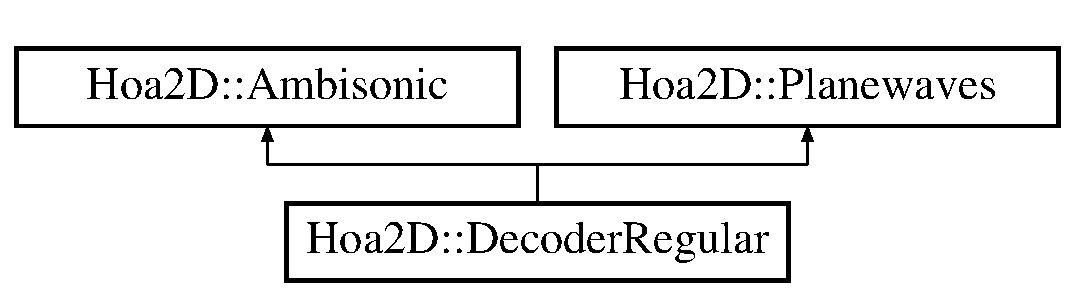
\includegraphics[height=2.000000cm]{class_hoa2_d_1_1_decoder_regular}
\end{center}
\end{figure}
\subsection*{Public Member Functions}
\begin{DoxyCompactItemize}
\item 
\hyperlink{class_hoa2_d_1_1_decoder_regular_a0666daa8b343e44ef7d90a31922cbecc}{Decoder\-Regular} (unsigned int order, unsigned int number\-Of\-Channels)
\begin{DoxyCompactList}\small\item\em The regular decoder constructor. \end{DoxyCompactList}\item 
\hyperlink{class_hoa2_d_1_1_decoder_regular_a04fe68432d2de773e8773cde9f0a2cad}{$\sim$\-Decoder\-Regular} ()
\begin{DoxyCompactList}\small\item\em The regular decoder destructor. \end{DoxyCompactList}\item 
void \hyperlink{class_hoa2_d_1_1_decoder_regular_a8ea45b4fafc13f941b597a7e829fc0d8}{set\-Channels\-Offset} (double offset)
\begin{DoxyCompactList}\small\item\em Set the offset of the channels. \end{DoxyCompactList}\item 
double \hyperlink{class_hoa2_d_1_1_decoder_regular_aa4dd9f25eac9fb517279cc310d9fe36f}{get\-Channels\-Offset} () const 
\begin{DoxyCompactList}\small\item\em Get the offset of the channels. \end{DoxyCompactList}\item 
void \hyperlink{class_hoa2_d_1_1_decoder_regular_a0df7ff818531d375909a2914d159b711}{process} (const float $\ast$input, float $\ast$output)
\begin{DoxyCompactList}\small\item\em This method performs the regular decoding with single precision. \end{DoxyCompactList}\item 
void \hyperlink{class_hoa2_d_1_1_decoder_regular_ab405af5dc134c282e25ca4d952bc0060}{process} (const double $\ast$input, double $\ast$output)
\begin{DoxyCompactList}\small\item\em This method performs the regular decoding with double precision. \end{DoxyCompactList}\end{DoxyCompactItemize}
\subsection*{Additional Inherited Members}


\subsection{Detailed Description}
The ambisonic regular decoder. 

The regular decoder should be used to decode an ambisonic sound field for a set a channels at equal distances on a circle depending on a decomposition order. The number of channels must be at least the number of harmonics. Note that you can only change the offset of the channels. 

Definition at line 19 of file Decoder.\-h.



\subsection{Constructor \& Destructor Documentation}
\hypertarget{class_hoa2_d_1_1_decoder_regular_a0666daa8b343e44ef7d90a31922cbecc}{\index{Hoa2\-D\-::\-Decoder\-Regular@{Hoa2\-D\-::\-Decoder\-Regular}!Decoder\-Regular@{Decoder\-Regular}}
\index{Decoder\-Regular@{Decoder\-Regular}!Hoa2D::DecoderRegular@{Hoa2\-D\-::\-Decoder\-Regular}}
\subsubsection[{Decoder\-Regular}]{\setlength{\rightskip}{0pt plus 5cm}Hoa2\-D\-::\-Decoder\-Regular\-::\-Decoder\-Regular (
\begin{DoxyParamCaption}
\item[{unsigned int}]{order, }
\item[{unsigned int}]{number\-Of\-Channels}
\end{DoxyParamCaption}
)}}\label{class_hoa2_d_1_1_decoder_regular_a0666daa8b343e44ef7d90a31922cbecc}


The regular decoder constructor. 

The regular decoder constructor allocates and initialize the member values to the decoding matrix depending of a decomposition order and a number of channels. The order must be at least 1 and the number of channels must be at least the number of harmonics.


\begin{DoxyParams}{Parameters}
{\em order} & The order \\
\hline
{\em number\-Of\-Channels} & The number of channels. \\
\hline
\end{DoxyParams}


Definition at line 14 of file Decoder.\-cpp.

\hypertarget{class_hoa2_d_1_1_decoder_regular_a04fe68432d2de773e8773cde9f0a2cad}{\index{Hoa2\-D\-::\-Decoder\-Regular@{Hoa2\-D\-::\-Decoder\-Regular}!$\sim$\-Decoder\-Regular@{$\sim$\-Decoder\-Regular}}
\index{$\sim$\-Decoder\-Regular@{$\sim$\-Decoder\-Regular}!Hoa2D::DecoderRegular@{Hoa2\-D\-::\-Decoder\-Regular}}
\subsubsection[{$\sim$\-Decoder\-Regular}]{\setlength{\rightskip}{0pt plus 5cm}Hoa2\-D\-::\-Decoder\-Regular\-::$\sim$\-Decoder\-Regular (
\begin{DoxyParamCaption}
{}
\end{DoxyParamCaption}
)}}\label{class_hoa2_d_1_1_decoder_regular_a04fe68432d2de773e8773cde9f0a2cad}


The regular decoder destructor. 

The regular decoder destructor free the memory. 

Definition at line 51 of file Decoder.\-cpp.



\subsection{Member Function Documentation}
\hypertarget{class_hoa2_d_1_1_decoder_regular_aa4dd9f25eac9fb517279cc310d9fe36f}{\index{Hoa2\-D\-::\-Decoder\-Regular@{Hoa2\-D\-::\-Decoder\-Regular}!get\-Channels\-Offset@{get\-Channels\-Offset}}
\index{get\-Channels\-Offset@{get\-Channels\-Offset}!Hoa2D::DecoderRegular@{Hoa2\-D\-::\-Decoder\-Regular}}
\subsubsection[{get\-Channels\-Offset}]{\setlength{\rightskip}{0pt plus 5cm}double Hoa2\-D\-::\-Decoder\-Regular\-::get\-Channels\-Offset (
\begin{DoxyParamCaption}
{}
\end{DoxyParamCaption}
) const\hspace{0.3cm}{\ttfamily [inline]}}}\label{class_hoa2_d_1_1_decoder_regular_aa4dd9f25eac9fb517279cc310d9fe36f}


Get the offset of the channels. 

Retreive the azimuth offset of the channels in radian.

\begin{DoxyReturn}{Returns}
The offset of the channels. 
\end{DoxyReturn}


Definition at line 56 of file Decoder.\-h.

\hypertarget{class_hoa2_d_1_1_decoder_regular_a0df7ff818531d375909a2914d159b711}{\index{Hoa2\-D\-::\-Decoder\-Regular@{Hoa2\-D\-::\-Decoder\-Regular}!process@{process}}
\index{process@{process}!Hoa2D::DecoderRegular@{Hoa2\-D\-::\-Decoder\-Regular}}
\subsubsection[{process}]{\setlength{\rightskip}{0pt plus 5cm}void Hoa2\-D\-::\-Decoder\-Regular\-::process (
\begin{DoxyParamCaption}
\item[{const float $\ast$}]{input, }
\item[{float $\ast$}]{output}
\end{DoxyParamCaption}
)}}\label{class_hoa2_d_1_1_decoder_regular_a0df7ff818531d375909a2914d159b711}


This method performs the regular decoding with single precision. 

You should use this method for in-\/place or not-\/in-\/place processing and performs the regular decoding sample by sample. The inputs array contains the spherical harmonics samples and the minimum size must be the number of harmonics and the outputs array contains the channels samples and the minimym size must be the number of channels.


\begin{DoxyParams}{Parameters}
{\em input} & The input sample. \\
\hline
{\em outputs} & The output array that contains samples destinated to channels. \\
\hline
\end{DoxyParams}


Definition at line 41 of file Decoder.\-cpp.

\hypertarget{class_hoa2_d_1_1_decoder_regular_ab405af5dc134c282e25ca4d952bc0060}{\index{Hoa2\-D\-::\-Decoder\-Regular@{Hoa2\-D\-::\-Decoder\-Regular}!process@{process}}
\index{process@{process}!Hoa2D::DecoderRegular@{Hoa2\-D\-::\-Decoder\-Regular}}
\subsubsection[{process}]{\setlength{\rightskip}{0pt plus 5cm}void Hoa2\-D\-::\-Decoder\-Regular\-::process (
\begin{DoxyParamCaption}
\item[{const double $\ast$}]{input, }
\item[{double $\ast$}]{output}
\end{DoxyParamCaption}
)}}\label{class_hoa2_d_1_1_decoder_regular_ab405af5dc134c282e25ca4d952bc0060}


This method performs the regular decoding with double precision. 

You should use this method for in-\/place or not-\/in-\/place processing and performs the regular decoding sample by sample. The inputs array contains the spherical harmonics samples and the minimum size must be the number of harmonics and the outputs array contains the channels samples and the minimym size must be the number of channels.


\begin{DoxyParams}{Parameters}
{\em input} & The input sample. \\
\hline
{\em outputs} & The output array that contains samples destinated to channels. \\
\hline
\end{DoxyParams}


Definition at line 46 of file Decoder.\-cpp.

\hypertarget{class_hoa2_d_1_1_decoder_regular_a8ea45b4fafc13f941b597a7e829fc0d8}{\index{Hoa2\-D\-::\-Decoder\-Regular@{Hoa2\-D\-::\-Decoder\-Regular}!set\-Channels\-Offset@{set\-Channels\-Offset}}
\index{set\-Channels\-Offset@{set\-Channels\-Offset}!Hoa2D::DecoderRegular@{Hoa2\-D\-::\-Decoder\-Regular}}
\subsubsection[{set\-Channels\-Offset}]{\setlength{\rightskip}{0pt plus 5cm}void Hoa2\-D\-::\-Decoder\-Regular\-::set\-Channels\-Offset (
\begin{DoxyParamCaption}
\item[{double}]{offset}
\end{DoxyParamCaption}
)}}\label{class_hoa2_d_1_1_decoder_regular_a8ea45b4fafc13f941b597a7e829fc0d8}


Set the offset of the channels. 

Set the azimuth offset of the channels in radian.


\begin{DoxyParams}{Parameters}
{\em offset} & An azimuth value. \\
\hline
\end{DoxyParams}


Definition at line 25 of file Decoder.\-cpp.



The documentation for this class was generated from the following files\-:\begin{DoxyCompactItemize}
\item 
/\-Users/elioton/\-Documents/programmation/\-C\-I\-C\-M/source\-Tree/\-Hoa\-Library/\-Sources/\-Hoa2\-D/Decoder.\-h\item 
/\-Users/elioton/\-Documents/programmation/\-C\-I\-C\-M/source\-Tree/\-Hoa\-Library/\-Sources/\-Hoa2\-D/Decoder.\-cpp\end{DoxyCompactItemize}

\hypertarget{class_hoa2_d_1_1_encoder}{\section{Hoa2\-D\-:\-:Encoder Class Reference}
\label{class_hoa2_d_1_1_encoder}\index{Hoa2\-D\-::\-Encoder@{Hoa2\-D\-::\-Encoder}}
}


The ambisonic encoder.  




{\ttfamily \#include $<$Encoder.\-h$>$}

Inheritance diagram for Hoa2\-D\-:\-:Encoder\-:\begin{figure}[H]
\begin{center}
\leavevmode
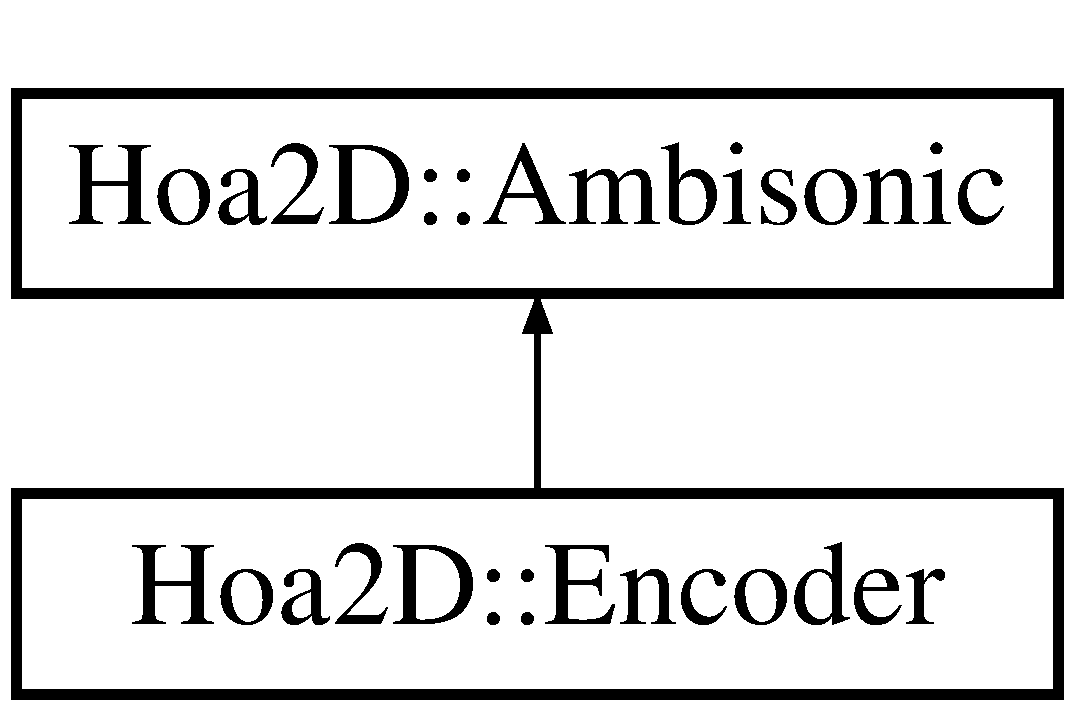
\includegraphics[height=2.000000cm]{class_hoa2_d_1_1_encoder}
\end{center}
\end{figure}
\subsection*{Public Member Functions}
\begin{DoxyCompactItemize}
\item 
\hyperlink{class_hoa2_d_1_1_encoder_a3387c0cd62d3af13ef851d5372c55a6f}{Encoder} (unsigned int order)
\begin{DoxyCompactList}\small\item\em The encoder constructor. \end{DoxyCompactList}\item 
\hyperlink{class_hoa2_d_1_1_encoder_a1faf86f0a74e68d91cd92608b5fd37c8}{$\sim$\-Encoder} ()
\begin{DoxyCompactList}\small\item\em The encoder destructor. \end{DoxyCompactList}\item 
void \hyperlink{class_hoa2_d_1_1_encoder_acc60cfd737fe1f0866e7d464ef1ec1f8}{set\-Azimuth} (const double azimuth)
\begin{DoxyCompactList}\small\item\em This method set the angle of azimuth. \end{DoxyCompactList}\item 
double \hyperlink{class_hoa2_d_1_1_encoder_a2ed07d913b444c58b3b1cf75dd1df117}{get\-Azimuth} () const 
\begin{DoxyCompactList}\small\item\em This method performs the encoding with single precision. \end{DoxyCompactList}\item 
void \hyperlink{class_hoa2_d_1_1_encoder_a2d12e80e9a7a59970972dca6b444b6bc}{process} (const float input, float $\ast$outputs)
\begin{DoxyCompactList}\small\item\em This method performs the encoding with single precision. \end{DoxyCompactList}\item 
void \hyperlink{class_hoa2_d_1_1_encoder_a235cc53dbf4fcbe71b3ea72a721eea81}{process} (const double input, double $\ast$outputs)
\begin{DoxyCompactList}\small\item\em This method performs the encoding with double precision. \end{DoxyCompactList}\end{DoxyCompactItemize}


\subsection{Detailed Description}
The ambisonic encoder. 

The encoder should be used to encode a signal in the spherical harmonics domain depending of an order of decomposition. It allows to control the azimuth of the encoding. 

Definition at line 17 of file Encoder.\-h.



\subsection{Constructor \& Destructor Documentation}
\hypertarget{class_hoa2_d_1_1_encoder_a3387c0cd62d3af13ef851d5372c55a6f}{\index{Hoa2\-D\-::\-Encoder@{Hoa2\-D\-::\-Encoder}!Encoder@{Encoder}}
\index{Encoder@{Encoder}!Hoa2D::Encoder@{Hoa2\-D\-::\-Encoder}}
\subsubsection[{Encoder}]{\setlength{\rightskip}{0pt plus 5cm}Hoa2\-D\-::\-Encoder\-::\-Encoder (
\begin{DoxyParamCaption}
\item[{unsigned int}]{order}
\end{DoxyParamCaption}
)}}\label{class_hoa2_d_1_1_encoder_a3387c0cd62d3af13ef851d5372c55a6f}


The encoder constructor. 

The encoder constructor allocates and initialize the member values to computes spherical harmonics coefficients depending of a decomposition order. The order must be at least 1.


\begin{DoxyParams}{Parameters}
{\em order} & The order. \\
\hline
\end{DoxyParams}


Definition at line 11 of file Encoder.\-cpp.

\hypertarget{class_hoa2_d_1_1_encoder_a1faf86f0a74e68d91cd92608b5fd37c8}{\index{Hoa2\-D\-::\-Encoder@{Hoa2\-D\-::\-Encoder}!$\sim$\-Encoder@{$\sim$\-Encoder}}
\index{$\sim$\-Encoder@{$\sim$\-Encoder}!Hoa2D::Encoder@{Hoa2\-D\-::\-Encoder}}
\subsubsection[{$\sim$\-Encoder}]{\setlength{\rightskip}{0pt plus 5cm}Hoa2\-D\-::\-Encoder\-::$\sim$\-Encoder (
\begin{DoxyParamCaption}
{}
\end{DoxyParamCaption}
)}}\label{class_hoa2_d_1_1_encoder_a1faf86f0a74e68d91cd92608b5fd37c8}


The encoder destructor. 

The encoder destructor free the memory. 

Definition at line 56 of file Encoder.\-cpp.



\subsection{Member Function Documentation}
\hypertarget{class_hoa2_d_1_1_encoder_a2ed07d913b444c58b3b1cf75dd1df117}{\index{Hoa2\-D\-::\-Encoder@{Hoa2\-D\-::\-Encoder}!get\-Azimuth@{get\-Azimuth}}
\index{get\-Azimuth@{get\-Azimuth}!Hoa2D::Encoder@{Hoa2\-D\-::\-Encoder}}
\subsubsection[{get\-Azimuth}]{\setlength{\rightskip}{0pt plus 5cm}double Hoa2\-D\-::\-Encoder\-::get\-Azimuth (
\begin{DoxyParamCaption}
{}
\end{DoxyParamCaption}
) const\hspace{0.3cm}{\ttfamily [inline]}}}\label{class_hoa2_d_1_1_encoder_a2ed07d913b444c58b3b1cf75dd1df117}


This method performs the encoding with single precision. 

You should use this method for in-\/place or not-\/in-\/place processing and performs the encoding sample by sample. The outputs array contains the spherical harmonics samples and the minimum size must be the number of harmonics.


\begin{DoxyParams}{Parameters}
{\em input} & The input sample. \\
\hline
{\em outputs} & The output array.\-Get the yaw value (rotation on the z-\/axis). The yaw is equivalent to a rotation on the z-\/axis (also named rotation).\\
\hline
\end{DoxyParams}
\begin{DoxyReturn}{Returns}
value The yaw value between 0 and 2π. 
\end{DoxyReturn}


Definition at line 59 of file Encoder.\-h.

\hypertarget{class_hoa2_d_1_1_encoder_a2d12e80e9a7a59970972dca6b444b6bc}{\index{Hoa2\-D\-::\-Encoder@{Hoa2\-D\-::\-Encoder}!process@{process}}
\index{process@{process}!Hoa2D::Encoder@{Hoa2\-D\-::\-Encoder}}
\subsubsection[{process}]{\setlength{\rightskip}{0pt plus 5cm}void Hoa2\-D\-::\-Encoder\-::process (
\begin{DoxyParamCaption}
\item[{const float}]{input, }
\item[{float $\ast$}]{outputs}
\end{DoxyParamCaption}
)}}\label{class_hoa2_d_1_1_encoder_a2d12e80e9a7a59970972dca6b444b6bc}


This method performs the encoding with single precision. 

\begin{DoxyVerb}You should use this method for in-place or not-in-place processing and performs the encoding sample by sample. The outputs array contains the spherical harmonics samples and the minimum size must be the number of harmonics.
\end{DoxyVerb}



\begin{DoxyParams}{Parameters}
{\em input} & The input sample. \\
\hline
{\em outputs} & The output array. \\
\hline
\end{DoxyParams}


Definition at line 24 of file Encoder.\-cpp.

\hypertarget{class_hoa2_d_1_1_encoder_a235cc53dbf4fcbe71b3ea72a721eea81}{\index{Hoa2\-D\-::\-Encoder@{Hoa2\-D\-::\-Encoder}!process@{process}}
\index{process@{process}!Hoa2D::Encoder@{Hoa2\-D\-::\-Encoder}}
\subsubsection[{process}]{\setlength{\rightskip}{0pt plus 5cm}void Hoa2\-D\-::\-Encoder\-::process (
\begin{DoxyParamCaption}
\item[{const double}]{input, }
\item[{double $\ast$}]{outputs}
\end{DoxyParamCaption}
)}}\label{class_hoa2_d_1_1_encoder_a235cc53dbf4fcbe71b3ea72a721eea81}


This method performs the encoding with double precision. 

You should use this method for in-\/place or not-\/in-\/place processing and performs the encoding sample by sample. The outputs array contains the spherical harmonics samples and the minimum size must be the number of harmonics.


\begin{DoxyParams}{Parameters}
{\em input} & The input sample. \\
\hline
{\em outputs} & The output array. \\
\hline
\end{DoxyParams}


Definition at line 40 of file Encoder.\-cpp.

\hypertarget{class_hoa2_d_1_1_encoder_acc60cfd737fe1f0866e7d464ef1ec1f8}{\index{Hoa2\-D\-::\-Encoder@{Hoa2\-D\-::\-Encoder}!set\-Azimuth@{set\-Azimuth}}
\index{set\-Azimuth@{set\-Azimuth}!Hoa2D::Encoder@{Hoa2\-D\-::\-Encoder}}
\subsubsection[{set\-Azimuth}]{\setlength{\rightskip}{0pt plus 5cm}void Hoa2\-D\-::\-Encoder\-::set\-Azimuth (
\begin{DoxyParamCaption}
\item[{const double}]{azimuth}
\end{DoxyParamCaption}
)}}\label{class_hoa2_d_1_1_encoder_acc60cfd737fe1f0866e7d464ef1ec1f8}


This method set the angle of azimuth. 

The angle of azimuth in radian and you should prefer to use it between 0 and 2 Pi to avoid recursive wrapping of the value. The direction of rotation is counterclockwise. The 0 radian is Pi/2 phase shifted relative to a mathematical representation of a circle, then the 0 radian is at the \char`\"{}front\char`\"{} of the soundfield.


\begin{DoxyParams}{Parameters}
{\em azimuth} & The azimuth. \\
\hline
\end{DoxyParams}


Definition at line 17 of file Encoder.\-cpp.



The documentation for this class was generated from the following files\-:\begin{DoxyCompactItemize}
\item 
/\-Users/\-Pierre/\-Source\-Tree/\-Hoa\-Library/\-Sources/\-Hoa2\-D/Encoder.\-h\item 
/\-Users/\-Pierre/\-Source\-Tree/\-Hoa\-Library/\-Sources/\-Hoa2\-D/Encoder.\-cpp\end{DoxyCompactItemize}

\hypertarget{class_hoa3_d_1_1_encoder}{\section{Hoa3\-D\-:\-:Encoder Class Reference}
\label{class_hoa3_d_1_1_encoder}\index{Hoa3\-D\-::\-Encoder@{Hoa3\-D\-::\-Encoder}}
}


The ambisonic encoder.  




{\ttfamily \#include $<$Encoder.\-h$>$}

Inheritance diagram for Hoa3\-D\-:\-:Encoder\-:\begin{figure}[H]
\begin{center}
\leavevmode
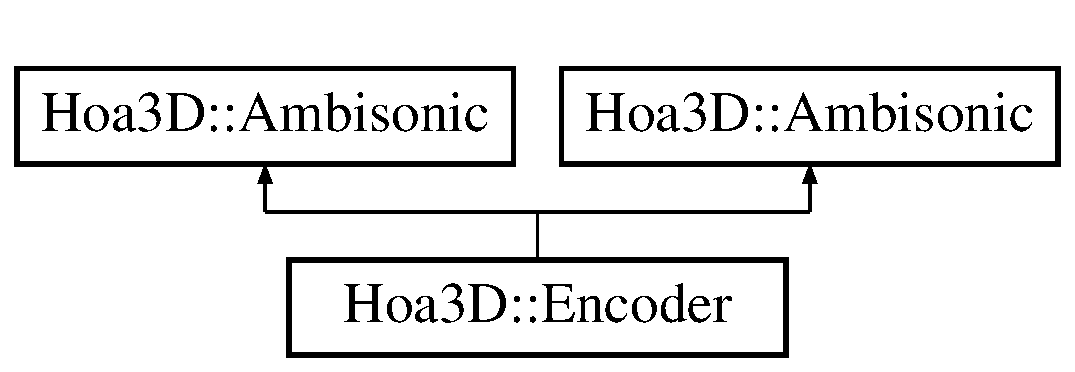
\includegraphics[height=2.000000cm]{class_hoa3_d_1_1_encoder}
\end{center}
\end{figure}
\subsection*{Public Member Functions}
\begin{DoxyCompactItemize}
\item 
\hyperlink{class_hoa3_d_1_1_encoder_a71052bcb0cbcf600852423c8cbbf29ce}{Encoder} (unsigned int order)
\begin{DoxyCompactList}\small\item\em The encoder constructor. \end{DoxyCompactList}\item 
\hyperlink{class_hoa3_d_1_1_encoder_a9842ee9f5abcba58a05a98dbfdff1b15}{$\sim$\-Encoder} ()
\begin{DoxyCompactList}\small\item\em The encoder destructor. \end{DoxyCompactList}\item 
void \hyperlink{class_hoa3_d_1_1_encoder_a7dbf4d5791003ed486fc0b5462409e0a}{set\-Azimuth} (const double azimuth)
\begin{DoxyCompactList}\small\item\em This method set the angle of azimuth. \end{DoxyCompactList}\item 
void \hyperlink{class_hoa3_d_1_1_encoder_a3bf01c6ecd90108c66c19ce7e5bde97d}{set\-Elevation} (const double elevation)
\begin{DoxyCompactList}\small\item\em This method set the angle of elevation. \end{DoxyCompactList}\item 
double \hyperlink{class_hoa3_d_1_1_encoder_a9887680a1cd725b96db8d83297922ae2}{get\-Normalization} (const unsigned int index) const 
\item 
void \hyperlink{class_hoa3_d_1_1_encoder_aedcd6cc5a50c85f373c61137e452a9b4}{process} (const float input, float $\ast$outputs)
\begin{DoxyCompactList}\small\item\em This method performs the encoding with single precision. \end{DoxyCompactList}\item 
void \hyperlink{class_hoa3_d_1_1_encoder_a6a8a7c7219424dd74bb5180a5b2c25e3}{process} (const double input, double $\ast$outputs)
\begin{DoxyCompactList}\small\item\em This method performs the encoding with double precision. \end{DoxyCompactList}\end{DoxyCompactItemize}


\subsection{Detailed Description}
The ambisonic encoder. 

The encoder should be used to encode a signal in the spherical harmonics domain depending of an order of decomposition. It allows to control the azimuth and the elevation of the encoding. If you want to spatialize with distance compensation, you should use the \hyperlink{class_hoa3_d_1_1_map}{Map} class.

\begin{DoxySeeAlso}{See Also}
\hyperlink{class_hoa3_d_1_1_map}{Map} 
\end{DoxySeeAlso}


Definition at line 19 of file Encoder.\-h.



\subsection{Constructor \& Destructor Documentation}
\hypertarget{class_hoa3_d_1_1_encoder_a71052bcb0cbcf600852423c8cbbf29ce}{\index{Hoa3\-D\-::\-Encoder@{Hoa3\-D\-::\-Encoder}!Encoder@{Encoder}}
\index{Encoder@{Encoder}!Hoa3D::Encoder@{Hoa3\-D\-::\-Encoder}}
\subsubsection[{Encoder}]{\setlength{\rightskip}{0pt plus 5cm}Hoa3\-D\-::\-Encoder\-::\-Encoder (
\begin{DoxyParamCaption}
\item[{unsigned int}]{order}
\end{DoxyParamCaption}
)}}\label{class_hoa3_d_1_1_encoder_a71052bcb0cbcf600852423c8cbbf29ce}


The encoder constructor. 

The encoder constructor allocates and initialize the member values to computes spherical harmonics coefficients depending of a decomposition order. The order must be at least 1.


\begin{DoxyParams}{Parameters}
{\em order} & The order. \\
\hline
\end{DoxyParams}


Definition at line 11 of file Encoder.\-cpp.

\hypertarget{class_hoa3_d_1_1_encoder_a9842ee9f5abcba58a05a98dbfdff1b15}{\index{Hoa3\-D\-::\-Encoder@{Hoa3\-D\-::\-Encoder}!$\sim$\-Encoder@{$\sim$\-Encoder}}
\index{$\sim$\-Encoder@{$\sim$\-Encoder}!Hoa3D::Encoder@{Hoa3\-D\-::\-Encoder}}
\subsubsection[{$\sim$\-Encoder}]{\setlength{\rightskip}{0pt plus 5cm}Hoa3\-D\-::\-Encoder\-::$\sim$\-Encoder (
\begin{DoxyParamCaption}
{}
\end{DoxyParamCaption}
)}}\label{class_hoa3_d_1_1_encoder_a9842ee9f5abcba58a05a98dbfdff1b15}


The encoder destructor. 

The encoder destructor free the memory. 

Definition at line 116 of file Encoder.\-cpp.



\subsection{Member Function Documentation}
\hypertarget{class_hoa3_d_1_1_encoder_a9887680a1cd725b96db8d83297922ae2}{\index{Hoa3\-D\-::\-Encoder@{Hoa3\-D\-::\-Encoder}!get\-Normalization@{get\-Normalization}}
\index{get\-Normalization@{get\-Normalization}!Hoa3D::Encoder@{Hoa3\-D\-::\-Encoder}}
\subsubsection[{get\-Normalization}]{\setlength{\rightskip}{0pt plus 5cm}double Hoa3\-D\-::\-Encoder\-::get\-Normalization (
\begin{DoxyParamCaption}
\item[{const unsigned int}]{index}
\end{DoxyParamCaption}
) const\hspace{0.3cm}{\ttfamily [inline]}}}\label{class_hoa3_d_1_1_encoder_a9887680a1cd725b96db8d83297922ae2}
Retreive the normalization of an harmonics


\begin{DoxyParams}{Parameters}
{\em index} & The index of the harmonics. \\
\hline
\end{DoxyParams}


Definition at line 63 of file Encoder.\-h.

\hypertarget{class_hoa3_d_1_1_encoder_aedcd6cc5a50c85f373c61137e452a9b4}{\index{Hoa3\-D\-::\-Encoder@{Hoa3\-D\-::\-Encoder}!process@{process}}
\index{process@{process}!Hoa3D::Encoder@{Hoa3\-D\-::\-Encoder}}
\subsubsection[{process}]{\setlength{\rightskip}{0pt plus 5cm}void Hoa3\-D\-::\-Encoder\-::process (
\begin{DoxyParamCaption}
\item[{const float}]{input, }
\item[{float $\ast$}]{outputs}
\end{DoxyParamCaption}
)}}\label{class_hoa3_d_1_1_encoder_aedcd6cc5a50c85f373c61137e452a9b4}


This method performs the encoding with single precision. 

You should use this method for in-\/place or not-\/in-\/place processing and performs the encoding sample by sample. The outputs array contains the spherical harmonics samples and the minimum size must be the number of harmonics.


\begin{DoxyParams}{Parameters}
{\em input} & The input sample. \\
\hline
{\em outputs} & The outputs array. \\
\hline
\end{DoxyParams}


Definition at line 70 of file Encoder.\-cpp.

\hypertarget{class_hoa3_d_1_1_encoder_a6a8a7c7219424dd74bb5180a5b2c25e3}{\index{Hoa3\-D\-::\-Encoder@{Hoa3\-D\-::\-Encoder}!process@{process}}
\index{process@{process}!Hoa3D::Encoder@{Hoa3\-D\-::\-Encoder}}
\subsubsection[{process}]{\setlength{\rightskip}{0pt plus 5cm}void Hoa3\-D\-::\-Encoder\-::process (
\begin{DoxyParamCaption}
\item[{const double}]{input, }
\item[{double $\ast$}]{outputs}
\end{DoxyParamCaption}
)}}\label{class_hoa3_d_1_1_encoder_a6a8a7c7219424dd74bb5180a5b2c25e3}


This method performs the encoding with double precision. 

You should use this method for in-\/place or not-\/in-\/place processing and performs the encoding sample by sample. The outputs array contains the spherical harmonics samples and the minimum size must be the number of harmonics.


\begin{DoxyParams}{Parameters}
{\em input} & The input sample. \\
\hline
{\em outputs} & The outputs array. \\
\hline
\end{DoxyParams}


Definition at line 92 of file Encoder.\-cpp.

\hypertarget{class_hoa3_d_1_1_encoder_a7dbf4d5791003ed486fc0b5462409e0a}{\index{Hoa3\-D\-::\-Encoder@{Hoa3\-D\-::\-Encoder}!set\-Azimuth@{set\-Azimuth}}
\index{set\-Azimuth@{set\-Azimuth}!Hoa3D::Encoder@{Hoa3\-D\-::\-Encoder}}
\subsubsection[{set\-Azimuth}]{\setlength{\rightskip}{0pt plus 5cm}void Hoa3\-D\-::\-Encoder\-::set\-Azimuth (
\begin{DoxyParamCaption}
\item[{const double}]{azimuth}
\end{DoxyParamCaption}
)}}\label{class_hoa3_d_1_1_encoder_a7dbf4d5791003ed486fc0b5462409e0a}


This method set the angle of azimuth. 

The angle of azimuth in radian and you should prefer to use it between 0 and 2 Pi to avoid recursive wrapping of the value. The direction of rotation is counterclockwise. The 0 radian is Pi/2 phase shifted relative to a mathematical representation of a circle, then the 0 radian is at the \char`\"{}front\char`\"{} of the soundfield.


\begin{DoxyParams}{Parameters}
{\em azimuth} & The azimuth. \\
\hline
\end{DoxyParams}
\begin{DoxySeeAlso}{See Also}
\hyperlink{class_hoa3_d_1_1_encoder_a3bf01c6ecd90108c66c19ce7e5bde97d}{set\-Elevation()} 
\end{DoxySeeAlso}


Definition at line 60 of file Encoder.\-cpp.

\hypertarget{class_hoa3_d_1_1_encoder_a3bf01c6ecd90108c66c19ce7e5bde97d}{\index{Hoa3\-D\-::\-Encoder@{Hoa3\-D\-::\-Encoder}!set\-Elevation@{set\-Elevation}}
\index{set\-Elevation@{set\-Elevation}!Hoa3D::Encoder@{Hoa3\-D\-::\-Encoder}}
\subsubsection[{set\-Elevation}]{\setlength{\rightskip}{0pt plus 5cm}void Hoa3\-D\-::\-Encoder\-::set\-Elevation (
\begin{DoxyParamCaption}
\item[{const double}]{elevation}
\end{DoxyParamCaption}
)}}\label{class_hoa3_d_1_1_encoder_a3bf01c6ecd90108c66c19ce7e5bde97d}


This method set the angle of elevation. 

The angle of elevation in radian and you should prefer to use it between 0 and 2 Pi to avoid recursive wrapping of the value. The direction of rotation is from bottom to the top. The 0 radian is centered at the \char`\"{}front\char`\"{} of the soundfield, then Pi/2 is at the top, -\/\-Pi/2 is at the bottom and Pi is behind. Note that if the angle of elevation is between Pi/2 and 3$\ast$\-Pi/2, the azimuth is reversed.


\begin{DoxyParams}{Parameters}
{\em elevation} & The elevation. \\
\hline
\end{DoxyParams}
\begin{DoxySeeAlso}{See Also}
\hyperlink{class_hoa3_d_1_1_encoder_a3bf01c6ecd90108c66c19ce7e5bde97d}{set\-Elevation()} 
\end{DoxySeeAlso}


Definition at line 65 of file Encoder.\-cpp.



The documentation for this class was generated from the following files\-:\begin{DoxyCompactItemize}
\item 
/\-Users/\-Pierre/\-Source\-Tree/\-Hoa\-Library/\-Sources/\-Hoa3\-D/Encoder.\-h\item 
/\-Users/\-Pierre/\-Source\-Tree/\-Hoa\-Library/\-Sources/\-Hoa3\-D/Encoder.\-cpp\end{DoxyCompactItemize}

\hypertarget{class_hoa3_d_1_1_map}{\section{Hoa3\-D\-:\-:Map Class Reference}
\label{class_hoa3_d_1_1_map}\index{Hoa3\-D\-::\-Map@{Hoa3\-D\-::\-Map}}
}


The ambisonic multi-\/encoder with distance compensation.  




{\ttfamily \#include $<$Map.\-h$>$}

Inheritance diagram for Hoa3\-D\-:\-:Map\-:\begin{figure}[H]
\begin{center}
\leavevmode
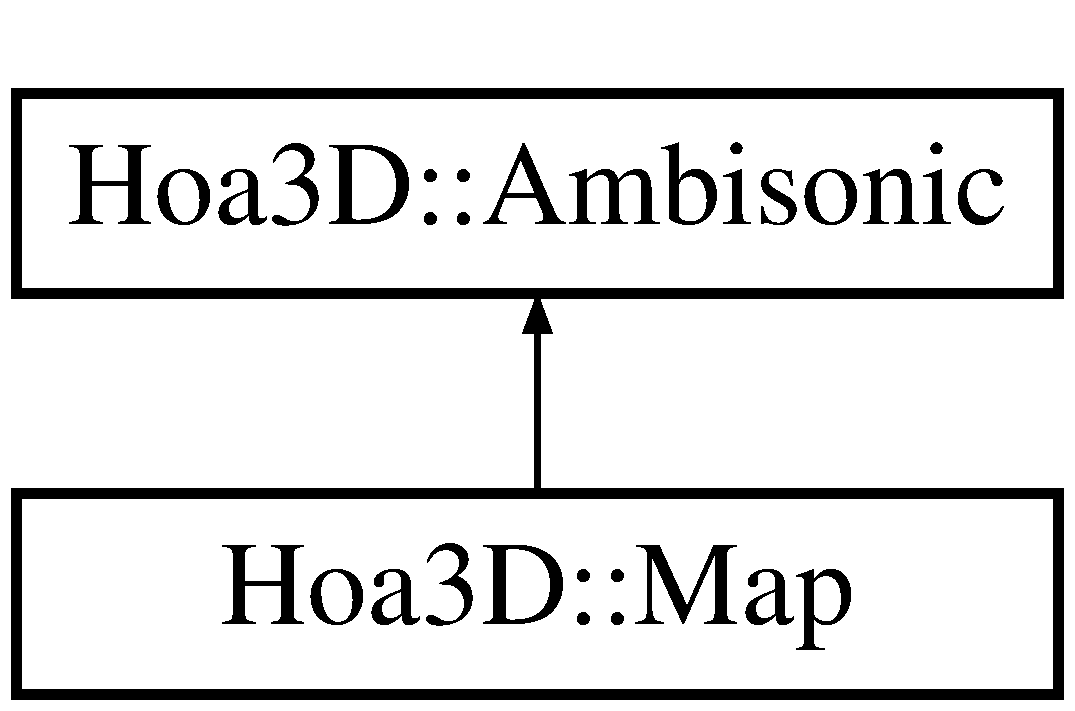
\includegraphics[height=2.000000cm]{class_hoa3_d_1_1_map}
\end{center}
\end{figure}
\subsection*{Public Member Functions}
\begin{DoxyCompactItemize}
\item 
\hyperlink{class_hoa3_d_1_1_map_a442cdcc3ac651b716ae2617fa64c44b4}{Map} (unsigned int order, unsigned int number\-Of\-Sources)
\begin{DoxyCompactList}\small\item\em The map constructor. \end{DoxyCompactList}\item 
\hyperlink{class_hoa3_d_1_1_map_a89f5772a7f26cda206637dd1fca1c16e}{$\sim$\-Map} ()
\begin{DoxyCompactList}\small\item\em The map destructor. \end{DoxyCompactList}\item 
void \hyperlink{class_hoa3_d_1_1_map_a251f215d1e137e652d12fc8e811bd8c8}{set\-Azimuth} (unsigned int index, const double azimuth)
\begin{DoxyCompactList}\small\item\em This method set the angle of azimuth of a source. \end{DoxyCompactList}\item 
void \hyperlink{class_hoa3_d_1_1_map_a03262a011f73ed57ba40bb6fe6d50814}{set\-Elevation} (unsigned int index, const double elevation)
\begin{DoxyCompactList}\small\item\em This method set the angle of elevation of a source. \end{DoxyCompactList}\item 
void \hyperlink{class_hoa3_d_1_1_map_a61b55ea17301701fc02dffca46957330}{set\-Distance} (unsigned int index, const double distance)
\begin{DoxyCompactList}\small\item\em This method set the diatnce of a source. \end{DoxyCompactList}\item 
unsigned int \hyperlink{class_hoa3_d_1_1_map_a49c97eaf507f6ccc9c1e7eb8fbff0ac9}{get\-Number\-Of\-Sources} () const 
\begin{DoxyCompactList}\small\item\em This method retrieve the number of sources. \end{DoxyCompactList}\item 
void \hyperlink{class_hoa3_d_1_1_map_af332c122731c3df55c3dcf56d39c7941}{process} (const float $\ast$inputs, float $\ast$outputs)
\begin{DoxyCompactList}\small\item\em This method performs the encoding with distance compensation with single precision. \end{DoxyCompactList}\item 
void \hyperlink{class_hoa3_d_1_1_map_a53a82b55c1ec5e52c2ab788984c5c2d0}{process} (const double $\ast$inputs, double $\ast$outputs)
\begin{DoxyCompactList}\small\item\em This method performs the encoding with distance compensation with double precision. \end{DoxyCompactList}\end{DoxyCompactItemize}


\subsection{Detailed Description}
The ambisonic multi-\/encoder with distance compensation. 

The map is a multi \hyperlink{class_hoa3_d_1_1_encoder}{Encoder} with distance compensation. It uses intances of the \hyperlink{class_hoa3_d_1_1_wider}{Wider} class to decrease the directionnality of sources by simulating fractionnal orders when the sources are inside the ambisonic sphere and a simple diminution of the gain when the sources get away from the ambisonic sphere.

\begin{DoxySeeAlso}{See Also}
\hyperlink{class_hoa3_d_1_1_encoder}{Encoder} 
\end{DoxySeeAlso}


Definition at line 21 of file Map.\-h.



\subsection{Constructor \& Destructor Documentation}
\hypertarget{class_hoa3_d_1_1_map_a442cdcc3ac651b716ae2617fa64c44b4}{\index{Hoa3\-D\-::\-Map@{Hoa3\-D\-::\-Map}!Map@{Map}}
\index{Map@{Map}!Hoa3D::Map@{Hoa3\-D\-::\-Map}}
\subsubsection[{Map}]{\setlength{\rightskip}{0pt plus 5cm}Hoa3\-D\-::\-Map\-::\-Map (
\begin{DoxyParamCaption}
\item[{unsigned int}]{order, }
\item[{unsigned int}]{number\-Of\-Sources}
\end{DoxyParamCaption}
)}}\label{class_hoa3_d_1_1_map_a442cdcc3ac651b716ae2617fa64c44b4}


The map constructor. 

The map constructor allocates and initialize the member values and classes depending of a decomposition order and the number of sources. The order and the number of sources must be at least 1.


\begin{DoxyParams}{Parameters}
{\em order} & The order. \\
\hline
{\em number\-Of\-Sources} & The number of sources. \\
\hline
\end{DoxyParams}


Definition at line 11 of file Map.\-cpp.

\hypertarget{class_hoa3_d_1_1_map_a89f5772a7f26cda206637dd1fca1c16e}{\index{Hoa3\-D\-::\-Map@{Hoa3\-D\-::\-Map}!$\sim$\-Map@{$\sim$\-Map}}
\index{$\sim$\-Map@{$\sim$\-Map}!Hoa3D::Map@{Hoa3\-D\-::\-Map}}
\subsubsection[{$\sim$\-Map}]{\setlength{\rightskip}{0pt plus 5cm}Hoa3\-D\-::\-Map\-::$\sim$\-Map (
\begin{DoxyParamCaption}
{}
\end{DoxyParamCaption}
)}}\label{class_hoa3_d_1_1_map_a89f5772a7f26cda206637dd1fca1c16e}


The map destructor. 

The map destructor free the memory and deallocate the member classes. 

Definition at line 77 of file Map.\-cpp.



\subsection{Member Function Documentation}
\hypertarget{class_hoa3_d_1_1_map_a49c97eaf507f6ccc9c1e7eb8fbff0ac9}{\index{Hoa3\-D\-::\-Map@{Hoa3\-D\-::\-Map}!get\-Number\-Of\-Sources@{get\-Number\-Of\-Sources}}
\index{get\-Number\-Of\-Sources@{get\-Number\-Of\-Sources}!Hoa3D::Map@{Hoa3\-D\-::\-Map}}
\subsubsection[{get\-Number\-Of\-Sources}]{\setlength{\rightskip}{0pt plus 5cm}unsigned int Hoa3\-D\-::\-Map\-::get\-Number\-Of\-Sources (
\begin{DoxyParamCaption}
{}
\end{DoxyParamCaption}
) const\hspace{0.3cm}{\ttfamily [inline]}}}\label{class_hoa3_d_1_1_map_a49c97eaf507f6ccc9c1e7eb8fbff0ac9}


This method retrieve the number of sources. 

Retrieve the number of sources.

\begin{DoxyReturn}{Returns}
The number of sources. 
\end{DoxyReturn}


Definition at line 83 of file Map.\-h.

\hypertarget{class_hoa3_d_1_1_map_af332c122731c3df55c3dcf56d39c7941}{\index{Hoa3\-D\-::\-Map@{Hoa3\-D\-::\-Map}!process@{process}}
\index{process@{process}!Hoa3D::Map@{Hoa3\-D\-::\-Map}}
\subsubsection[{process}]{\setlength{\rightskip}{0pt plus 5cm}void Hoa3\-D\-::\-Map\-::process (
\begin{DoxyParamCaption}
\item[{const float $\ast$}]{inputs, }
\item[{float $\ast$}]{outputs}
\end{DoxyParamCaption}
)}}\label{class_hoa3_d_1_1_map_af332c122731c3df55c3dcf56d39c7941}


This method performs the encoding with distance compensation with single precision. 

You should use this method for in-\/place or not-\/in-\/place processing and performs the encoding with distance compensation sample by sample. The inputs array contains the samples of the sources and the minimum size sould be the number of sources. The outputs array contains the spherical harmonics samples and the minimum size must be the number of harmonics.


\begin{DoxyParams}{Parameters}
{\em inputs} & The inputs array. \\
\hline
{\em outputs} & The outputs array. \\
\hline
\end{DoxyParams}


Definition at line 53 of file Map.\-cpp.

\hypertarget{class_hoa3_d_1_1_map_a53a82b55c1ec5e52c2ab788984c5c2d0}{\index{Hoa3\-D\-::\-Map@{Hoa3\-D\-::\-Map}!process@{process}}
\index{process@{process}!Hoa3D::Map@{Hoa3\-D\-::\-Map}}
\subsubsection[{process}]{\setlength{\rightskip}{0pt plus 5cm}void Hoa3\-D\-::\-Map\-::process (
\begin{DoxyParamCaption}
\item[{const double $\ast$}]{inputs, }
\item[{double $\ast$}]{outputs}
\end{DoxyParamCaption}
)}}\label{class_hoa3_d_1_1_map_a53a82b55c1ec5e52c2ab788984c5c2d0}


This method performs the encoding with distance compensation with double precision. 

You should use this method for in-\/place or not-\/in-\/place processing and performs the encoding with distance compensation sample by sample. The inputs array contains the samples of the sources and the minimum size sould be the number of sources. The outputs array contains the spherical harmonics samples and the minimum size must be the number of harmonics.


\begin{DoxyParams}{Parameters}
{\em inputs} & The inputs array. \\
\hline
{\em outputs} & The outputs array. \\
\hline
\end{DoxyParams}


Definition at line 65 of file Map.\-cpp.

\hypertarget{class_hoa3_d_1_1_map_a251f215d1e137e652d12fc8e811bd8c8}{\index{Hoa3\-D\-::\-Map@{Hoa3\-D\-::\-Map}!set\-Azimuth@{set\-Azimuth}}
\index{set\-Azimuth@{set\-Azimuth}!Hoa3D::Map@{Hoa3\-D\-::\-Map}}
\subsubsection[{set\-Azimuth}]{\setlength{\rightskip}{0pt plus 5cm}void Hoa3\-D\-::\-Map\-::set\-Azimuth (
\begin{DoxyParamCaption}
\item[{unsigned int}]{index, }
\item[{const double}]{azimuth}
\end{DoxyParamCaption}
)}}\label{class_hoa3_d_1_1_map_a251f215d1e137e652d12fc8e811bd8c8}


This method set the angle of azimuth of a source. 

The angle of azimuth in radian, look at the \hyperlink{class_hoa3_d_1_1_encoder}{Encoder} for further informations. The index must be between 0 and the number of sources.


\begin{DoxyParams}{Parameters}
{\em index} & The index of the source. \\
\hline
{\em azimuth} & The azimuth. \\
\hline
\end{DoxyParams}
\begin{DoxySeeAlso}{See Also}
\hyperlink{class_hoa3_d_1_1_map_a03262a011f73ed57ba40bb6fe6d50814}{set\-Elevation()} 

\hyperlink{class_hoa3_d_1_1_map_a61b55ea17301701fc02dffca46957330}{set\-Distance()} 
\end{DoxySeeAlso}


Definition at line 26 of file Map.\-cpp.

\hypertarget{class_hoa3_d_1_1_map_a61b55ea17301701fc02dffca46957330}{\index{Hoa3\-D\-::\-Map@{Hoa3\-D\-::\-Map}!set\-Distance@{set\-Distance}}
\index{set\-Distance@{set\-Distance}!Hoa3D::Map@{Hoa3\-D\-::\-Map}}
\subsubsection[{set\-Distance}]{\setlength{\rightskip}{0pt plus 5cm}void Hoa3\-D\-::\-Map\-::set\-Distance (
\begin{DoxyParamCaption}
\item[{unsigned int}]{index, }
\item[{const double}]{distance}
\end{DoxyParamCaption}
)}}\label{class_hoa3_d_1_1_map_a61b55ea17301701fc02dffca46957330}


This method set the diatnce of a source. 

The distance is between 0 and infinity. At 0, the source is in the center of the ambisonic sphere and at 1, the source is at the surface of the ambisonic sphere. Over 1, the source get away the ambisonic sphere. The index must be between 0 and the number of sources.


\begin{DoxyParams}{Parameters}
{\em index} & The index of the source. \\
\hline
{\em elevation} & The elevation. \\
\hline
\end{DoxyParams}
\begin{DoxySeeAlso}{See Also}
\hyperlink{class_hoa3_d_1_1_map_a251f215d1e137e652d12fc8e811bd8c8}{set\-Azimuth()} 

\hyperlink{class_hoa3_d_1_1_map_a03262a011f73ed57ba40bb6fe6d50814}{set\-Elevation()} 
\end{DoxySeeAlso}


Definition at line 38 of file Map.\-cpp.

\hypertarget{class_hoa3_d_1_1_map_a03262a011f73ed57ba40bb6fe6d50814}{\index{Hoa3\-D\-::\-Map@{Hoa3\-D\-::\-Map}!set\-Elevation@{set\-Elevation}}
\index{set\-Elevation@{set\-Elevation}!Hoa3D::Map@{Hoa3\-D\-::\-Map}}
\subsubsection[{set\-Elevation}]{\setlength{\rightskip}{0pt plus 5cm}void Hoa3\-D\-::\-Map\-::set\-Elevation (
\begin{DoxyParamCaption}
\item[{unsigned int}]{index, }
\item[{const double}]{elevation}
\end{DoxyParamCaption}
)}}\label{class_hoa3_d_1_1_map_a03262a011f73ed57ba40bb6fe6d50814}


This method set the angle of elevation of a source. 

The angle of elevation in radian, look at the \hyperlink{class_hoa3_d_1_1_encoder}{Encoder} for further informations. The index must be between 0 and the number of sources.


\begin{DoxyParams}{Parameters}
{\em index} & The index of the source. \\
\hline
{\em elevation} & The elevation. \\
\hline
\end{DoxyParams}
\begin{DoxySeeAlso}{See Also}
\hyperlink{class_hoa3_d_1_1_map_a251f215d1e137e652d12fc8e811bd8c8}{set\-Azimuth()} 

\hyperlink{class_hoa3_d_1_1_map_a61b55ea17301701fc02dffca46957330}{set\-Distance()} 
\end{DoxySeeAlso}


Definition at line 32 of file Map.\-cpp.



The documentation for this class was generated from the following files\-:\begin{DoxyCompactItemize}
\item 
/\-Users/elioton/\-Documents/programmation/\-C\-I\-C\-M/source\-Tree/\-Hoa\-Library/\-Sources/\-Hoa3\-D/Map.\-h\item 
/\-Users/elioton/\-Documents/programmation/\-C\-I\-C\-M/source\-Tree/\-Hoa\-Library/\-Sources/\-Hoa3\-D/Map.\-cpp\end{DoxyCompactItemize}

\hypertarget{class_hoa2_d_1_1_map}{\section{Hoa2\-D\-:\-:Map Class Reference}
\label{class_hoa2_d_1_1_map}\index{Hoa2\-D\-::\-Map@{Hoa2\-D\-::\-Map}}
}


The ambisonic multi-\/encoder with distance compensation.  




{\ttfamily \#include $<$Map.\-h$>$}

Inheritance diagram for Hoa2\-D\-:\-:Map\-:\begin{figure}[H]
\begin{center}
\leavevmode
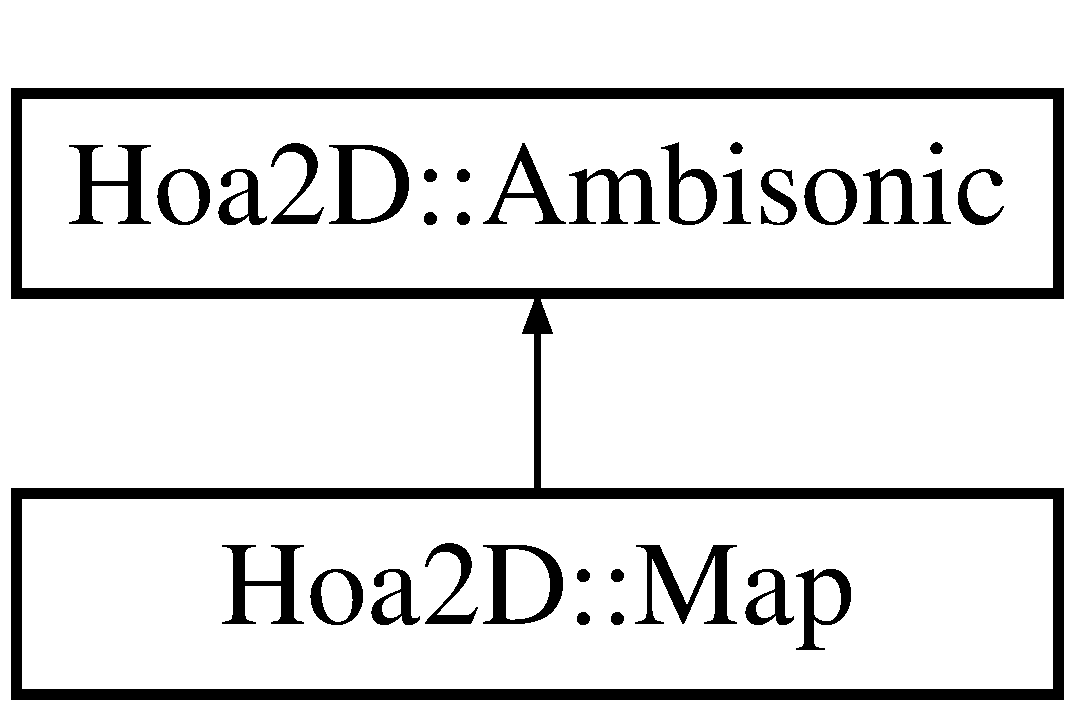
\includegraphics[height=2.000000cm]{class_hoa2_d_1_1_map}
\end{center}
\end{figure}
\subsection*{Public Member Functions}
\begin{DoxyCompactItemize}
\item 
\hyperlink{class_hoa2_d_1_1_map_a22720e5b9ab041bb970d4dc43086558c}{Map} (unsigned int order, unsigned int number\-Of\-Sources)
\begin{DoxyCompactList}\small\item\em The map constructor. \end{DoxyCompactList}\item 
\hyperlink{class_hoa2_d_1_1_map_a47d01e332e6c19015e9fd94e8898f4f3}{$\sim$\-Map} ()
\begin{DoxyCompactList}\small\item\em The map destructor. \end{DoxyCompactList}\item 
unsigned int \hyperlink{class_hoa2_d_1_1_map_aef1bab3391d2292182a9b8205200e9af}{get\-Number\-Of\-Sources} () const 
\begin{DoxyCompactList}\small\item\em This method retrieve the number of sources. \end{DoxyCompactList}\item 
void \hyperlink{class_hoa2_d_1_1_map_aa5e77ccf4d3e2aaf75162180c18e202d}{set\-Azimuth} (const unsigned int index, const double azimuth)
\begin{DoxyCompactList}\small\item\em This method set the angle of azimuth of a source. \end{DoxyCompactList}\item 
void \hyperlink{class_hoa2_d_1_1_map_a48b9f89f5fcdab909f1fd50a7256a9f0}{set\-Radius} (const unsigned int index, const double radius)
\begin{DoxyCompactList}\small\item\em This method set the radius of a source. \end{DoxyCompactList}\item 
void \hyperlink{class_hoa2_d_1_1_map_a318a974ce6e0d5607a2fe4973093c9b9}{set\-Mute} (const unsigned int index, const bool muted)
\begin{DoxyCompactList}\small\item\em This method mute or unmute a source. \end{DoxyCompactList}\item 
double \hyperlink{class_hoa2_d_1_1_map_ae53d58090226e3139fccb8a75249bc3b}{get\-Azimuth} (const unsigned int index) const 
\begin{DoxyCompactList}\small\item\em This method retrieve the azimuth of a source. \end{DoxyCompactList}\item 
double \hyperlink{class_hoa2_d_1_1_map_a10d0058386c2738f6e11584c9e751c83}{get\-Radius} (const unsigned int index) const 
\begin{DoxyCompactList}\small\item\em This method retrieve the radius of a source. \end{DoxyCompactList}\item 
bool \hyperlink{class_hoa2_d_1_1_map_af3d625389cbce9e5e46a4532e39e2c5e}{get\-Mute} (const unsigned int index, const bool muted) const 
\begin{DoxyCompactList}\small\item\em This method retrieve the mute or unmute state of a source. \end{DoxyCompactList}\item 
void \hyperlink{class_hoa2_d_1_1_map_a933daf1cc1c8ad4df486d436f6d91450}{process} (const float $\ast$inputs, float $\ast$outputs)
\begin{DoxyCompactList}\small\item\em This method performs the encoding with distance compensation with single precision. \end{DoxyCompactList}\item 
void \hyperlink{class_hoa2_d_1_1_map_aa71ff518d419b54b409043ded7b8abd4}{process} (const double $\ast$inputs, double $\ast$outputs)
\begin{DoxyCompactList}\small\item\em This method performs the encoding with distance compensation with double precision. \end{DoxyCompactList}\end{DoxyCompactItemize}


\subsection{Detailed Description}
The ambisonic multi-\/encoder with distance compensation. 

The map is a multi \hyperlink{class_hoa2_d_1_1_encoder}{Encoder} with distance compensation. It uses intances of the \hyperlink{class_hoa2_d_1_1_wider}{Wider} class to decrease the directionnality of sources by simulating fractionnal orders when the sources are inside the ambisonic circle and a simple diminution of the gain when the sources get away from the ambisonic circle.

\begin{DoxySeeAlso}{See Also}
\hyperlink{class_hoa2_d_1_1_encoder}{Encoder} 
\end{DoxySeeAlso}


Definition at line 21 of file Map.\-h.



\subsection{Constructor \& Destructor Documentation}
\hypertarget{class_hoa2_d_1_1_map_a22720e5b9ab041bb970d4dc43086558c}{\index{Hoa2\-D\-::\-Map@{Hoa2\-D\-::\-Map}!Map@{Map}}
\index{Map@{Map}!Hoa2D::Map@{Hoa2\-D\-::\-Map}}
\subsubsection[{Map}]{\setlength{\rightskip}{0pt plus 5cm}Hoa2\-D\-::\-Map\-::\-Map (
\begin{DoxyParamCaption}
\item[{unsigned int}]{order, }
\item[{unsigned int}]{number\-Of\-Sources}
\end{DoxyParamCaption}
)}}\label{class_hoa2_d_1_1_map_a22720e5b9ab041bb970d4dc43086558c}


The map constructor. 

The map constructor allocates and initialize the member values and classes depending of a decomposition order and the number of sources. The order and the number of sources must be at least 1.


\begin{DoxyParams}{Parameters}
{\em order} & The order. \\
\hline
{\em number\-Of\-Sources} & The number of sources. \\
\hline
\end{DoxyParams}


Definition at line 11 of file Map.\-cpp.

\hypertarget{class_hoa2_d_1_1_map_a47d01e332e6c19015e9fd94e8898f4f3}{\index{Hoa2\-D\-::\-Map@{Hoa2\-D\-::\-Map}!$\sim$\-Map@{$\sim$\-Map}}
\index{$\sim$\-Map@{$\sim$\-Map}!Hoa2D::Map@{Hoa2\-D\-::\-Map}}
\subsubsection[{$\sim$\-Map}]{\setlength{\rightskip}{0pt plus 5cm}Hoa2\-D\-::\-Map\-::$\sim$\-Map (
\begin{DoxyParamCaption}
{}
\end{DoxyParamCaption}
)}}\label{class_hoa2_d_1_1_map_a47d01e332e6c19015e9fd94e8898f4f3}


The map destructor. 

The map destructor free the memory and deallocate the member classes. 

Definition at line 113 of file Map.\-cpp.



\subsection{Member Function Documentation}
\hypertarget{class_hoa2_d_1_1_map_ae53d58090226e3139fccb8a75249bc3b}{\index{Hoa2\-D\-::\-Map@{Hoa2\-D\-::\-Map}!get\-Azimuth@{get\-Azimuth}}
\index{get\-Azimuth@{get\-Azimuth}!Hoa2D::Map@{Hoa2\-D\-::\-Map}}
\subsubsection[{get\-Azimuth}]{\setlength{\rightskip}{0pt plus 5cm}double Hoa2\-D\-::\-Map\-::get\-Azimuth (
\begin{DoxyParamCaption}
\item[{const unsigned int}]{index}
\end{DoxyParamCaption}
) const\hspace{0.3cm}{\ttfamily [inline]}}}\label{class_hoa2_d_1_1_map_ae53d58090226e3139fccb8a75249bc3b}


This method retrieve the azimuth of a source. 

Retrieve the azimuth of a source.


\begin{DoxyParams}{Parameters}
{\em index} & The index of the source. \\
\hline
\end{DoxyParams}
\begin{DoxyReturn}{Returns}
The azimuth of the source if the source exists, otherwise the function generates an error. 
\end{DoxyReturn}


Definition at line 92 of file Map.\-h.

\hypertarget{class_hoa2_d_1_1_map_af3d625389cbce9e5e46a4532e39e2c5e}{\index{Hoa2\-D\-::\-Map@{Hoa2\-D\-::\-Map}!get\-Mute@{get\-Mute}}
\index{get\-Mute@{get\-Mute}!Hoa2D::Map@{Hoa2\-D\-::\-Map}}
\subsubsection[{get\-Mute}]{\setlength{\rightskip}{0pt plus 5cm}bool Hoa2\-D\-::\-Map\-::get\-Mute (
\begin{DoxyParamCaption}
\item[{const unsigned int}]{index, }
\item[{const bool}]{muted}
\end{DoxyParamCaption}
) const\hspace{0.3cm}{\ttfamily [inline]}}}\label{class_hoa2_d_1_1_map_af3d625389cbce9e5e46a4532e39e2c5e}


This method retrieve the mute or unmute state of a source. 

Get the Mute state of a source.


\begin{DoxyParams}{Parameters}
{\em index} & The index of the source. \\
\hline
\end{DoxyParams}
\begin{DoxyReturn}{Returns}
The mute state of the source if the source exists, otherwise the function generates an error. 
\end{DoxyReturn}
\begin{DoxySeeAlso}{See Also}
\hyperlink{class_hoa2_d_1_1_map_a318a974ce6e0d5607a2fe4973093c9b9}{set\-Mute()} 
\end{DoxySeeAlso}


Definition at line 120 of file Map.\-h.

\hypertarget{class_hoa2_d_1_1_map_aef1bab3391d2292182a9b8205200e9af}{\index{Hoa2\-D\-::\-Map@{Hoa2\-D\-::\-Map}!get\-Number\-Of\-Sources@{get\-Number\-Of\-Sources}}
\index{get\-Number\-Of\-Sources@{get\-Number\-Of\-Sources}!Hoa2D::Map@{Hoa2\-D\-::\-Map}}
\subsubsection[{get\-Number\-Of\-Sources}]{\setlength{\rightskip}{0pt plus 5cm}unsigned int Hoa2\-D\-::\-Map\-::get\-Number\-Of\-Sources (
\begin{DoxyParamCaption}
{}
\end{DoxyParamCaption}
) const\hspace{0.3cm}{\ttfamily [inline]}}}\label{class_hoa2_d_1_1_map_aef1bab3391d2292182a9b8205200e9af}


This method retrieve the number of sources. 

Retrieve the number of sources.

\begin{DoxyReturn}{Returns}
The number of sources. 
\end{DoxyReturn}


Definition at line 55 of file Map.\-h.

\hypertarget{class_hoa2_d_1_1_map_a10d0058386c2738f6e11584c9e751c83}{\index{Hoa2\-D\-::\-Map@{Hoa2\-D\-::\-Map}!get\-Radius@{get\-Radius}}
\index{get\-Radius@{get\-Radius}!Hoa2D::Map@{Hoa2\-D\-::\-Map}}
\subsubsection[{get\-Radius}]{\setlength{\rightskip}{0pt plus 5cm}double Hoa2\-D\-::\-Map\-::get\-Radius (
\begin{DoxyParamCaption}
\item[{const unsigned int}]{index}
\end{DoxyParamCaption}
) const\hspace{0.3cm}{\ttfamily [inline]}}}\label{class_hoa2_d_1_1_map_a10d0058386c2738f6e11584c9e751c83}


This method retrieve the radius of a source. 

Retrieve the radius of a source.


\begin{DoxyParams}{Parameters}
{\em index} & The index of the source. \\
\hline
\end{DoxyParams}
\begin{DoxyReturn}{Returns}
The radius of the source if the source exists, otherwise the function generates an error. 
\end{DoxyReturn}


Definition at line 104 of file Map.\-h.

\hypertarget{class_hoa2_d_1_1_map_a933daf1cc1c8ad4df486d436f6d91450}{\index{Hoa2\-D\-::\-Map@{Hoa2\-D\-::\-Map}!process@{process}}
\index{process@{process}!Hoa2D::Map@{Hoa2\-D\-::\-Map}}
\subsubsection[{process}]{\setlength{\rightskip}{0pt plus 5cm}void Hoa2\-D\-::\-Map\-::process (
\begin{DoxyParamCaption}
\item[{const float $\ast$}]{inputs, }
\item[{float $\ast$}]{outputs}
\end{DoxyParamCaption}
)}}\label{class_hoa2_d_1_1_map_a933daf1cc1c8ad4df486d436f6d91450}


This method performs the encoding with distance compensation with single precision. 

\begin{DoxyVerb}You should use this method for in-place or not-in-place processing and performs the encoding with distance compensation sample by sample. The inputs array contains the samples of the sources and the minimum size sould be the number of sources. The outputs array contains the spherical harmonics samples and the minimum size must be the number of harmonics.
\end{DoxyVerb}



\begin{DoxyParams}{Parameters}
{\em inputs} & The inputs array. \\
\hline
{\em outputs} & The outputs array. \\
\hline
\end{DoxyParams}


Definition at line 66 of file Map.\-cpp.

\hypertarget{class_hoa2_d_1_1_map_aa71ff518d419b54b409043ded7b8abd4}{\index{Hoa2\-D\-::\-Map@{Hoa2\-D\-::\-Map}!process@{process}}
\index{process@{process}!Hoa2D::Map@{Hoa2\-D\-::\-Map}}
\subsubsection[{process}]{\setlength{\rightskip}{0pt plus 5cm}void Hoa2\-D\-::\-Map\-::process (
\begin{DoxyParamCaption}
\item[{const double $\ast$}]{inputs, }
\item[{double $\ast$}]{outputs}
\end{DoxyParamCaption}
)}}\label{class_hoa2_d_1_1_map_aa71ff518d419b54b409043ded7b8abd4}


This method performs the encoding with distance compensation with double precision. 

You should use this method for in-\/place or not-\/in-\/place processing and performs the encoding with distance compensation sample by sample. The inputs array contains the samples of the sources and the minimum size sould be the number of sources. The outputs array contains the spherical harmonics samples and the minimum size must be the number of harmonics.


\begin{DoxyParams}{Parameters}
{\em inputs} & The inputs array. \\
\hline
{\em outputs} & The outputs array. \\
\hline
\end{DoxyParams}


Definition at line 89 of file Map.\-cpp.

\hypertarget{class_hoa2_d_1_1_map_aa5e77ccf4d3e2aaf75162180c18e202d}{\index{Hoa2\-D\-::\-Map@{Hoa2\-D\-::\-Map}!set\-Azimuth@{set\-Azimuth}}
\index{set\-Azimuth@{set\-Azimuth}!Hoa2D::Map@{Hoa2\-D\-::\-Map}}
\subsubsection[{set\-Azimuth}]{\setlength{\rightskip}{0pt plus 5cm}void Hoa2\-D\-::\-Map\-::set\-Azimuth (
\begin{DoxyParamCaption}
\item[{const unsigned int}]{index, }
\item[{const double}]{azimuth}
\end{DoxyParamCaption}
)}}\label{class_hoa2_d_1_1_map_aa5e77ccf4d3e2aaf75162180c18e202d}


This method set the angle of azimuth of a source. 

The angle of azimuth in radian and you should prefer to use it between 0 and 2 Pi to avoid recursive wrapping of the value. The direction of rotation is counterclockwise. The 0 radian is Pi/2 phase shifted relative to a mathematical representation of a circle, then the 0 radian is at the \char`\"{}front\char`\"{} of the soundfield. The index must be between 0 and the number of sources -\/ 1.


\begin{DoxyParams}{Parameters}
{\em index} & The index of the source. \\
\hline
{\em azimuth} & The azimuth. \\
\hline
\end{DoxyParams}
\begin{DoxySeeAlso}{See Also}
\hyperlink{class_hoa2_d_1_1_map_a48b9f89f5fcdab909f1fd50a7256a9f0}{set\-Radius()} 
\end{DoxySeeAlso}


Definition at line 30 of file Map.\-cpp.

\hypertarget{class_hoa2_d_1_1_map_a318a974ce6e0d5607a2fe4973093c9b9}{\index{Hoa2\-D\-::\-Map@{Hoa2\-D\-::\-Map}!set\-Mute@{set\-Mute}}
\index{set\-Mute@{set\-Mute}!Hoa2D::Map@{Hoa2\-D\-::\-Map}}
\subsubsection[{set\-Mute}]{\setlength{\rightskip}{0pt plus 5cm}void Hoa2\-D\-::\-Map\-::set\-Mute (
\begin{DoxyParamCaption}
\item[{const unsigned int}]{index, }
\item[{const bool}]{muted}
\end{DoxyParamCaption}
)}}\label{class_hoa2_d_1_1_map_a318a974ce6e0d5607a2fe4973093c9b9}


This method mute or unmute a source. 

Mute or unmute a source with a boolean value. The index must be between 0 and the number of sources -\/ 1.


\begin{DoxyParams}{Parameters}
{\em index} & The index of the source. \\
\hline
{\em muted} & The mute state. \\
\hline
\end{DoxyParams}


Definition at line 51 of file Map.\-cpp.

\hypertarget{class_hoa2_d_1_1_map_a48b9f89f5fcdab909f1fd50a7256a9f0}{\index{Hoa2\-D\-::\-Map@{Hoa2\-D\-::\-Map}!set\-Radius@{set\-Radius}}
\index{set\-Radius@{set\-Radius}!Hoa2D::Map@{Hoa2\-D\-::\-Map}}
\subsubsection[{set\-Radius}]{\setlength{\rightskip}{0pt plus 5cm}void Hoa2\-D\-::\-Map\-::set\-Radius (
\begin{DoxyParamCaption}
\item[{const unsigned int}]{index, }
\item[{const double}]{radius}
\end{DoxyParamCaption}
)}}\label{class_hoa2_d_1_1_map_a48b9f89f5fcdab909f1fd50a7256a9f0}


This method set the radius of a source. 

The radius is between 0 and infinity. At 0, the source is in the center of the ambisonic circle and at 1, the source is at the limit of the ambisonic circle. Over 1, the source get away the ambisonic circle. The index must be between 0 and the number of sources -\/ 1.


\begin{DoxyParams}{Parameters}
{\em index} & The index of the source. \\
\hline
{\em radius} & The radius. \\
\hline
\end{DoxyParams}
\begin{DoxySeeAlso}{See Also}
\hyperlink{class_hoa2_d_1_1_map_aa5e77ccf4d3e2aaf75162180c18e202d}{set\-Azimuth()} 
\end{DoxySeeAlso}


Definition at line 36 of file Map.\-cpp.


\hypertarget{class_hoa3_d_1_1_meter}{\section{Hoa3\-D\-:\-:Meter Class Reference}
\label{class_hoa3_d_1_1_meter}\index{Hoa3\-D\-::\-Meter@{Hoa3\-D\-::\-Meter}}
}


The ambisonic \hyperlink{class_hoa3_d_1_1_meter}{Meter}.  




{\ttfamily \#include $<$Meter.\-h$>$}

Inheritance diagram for Hoa3\-D\-:\-:Meter\-:\begin{figure}[H]
\begin{center}
\leavevmode
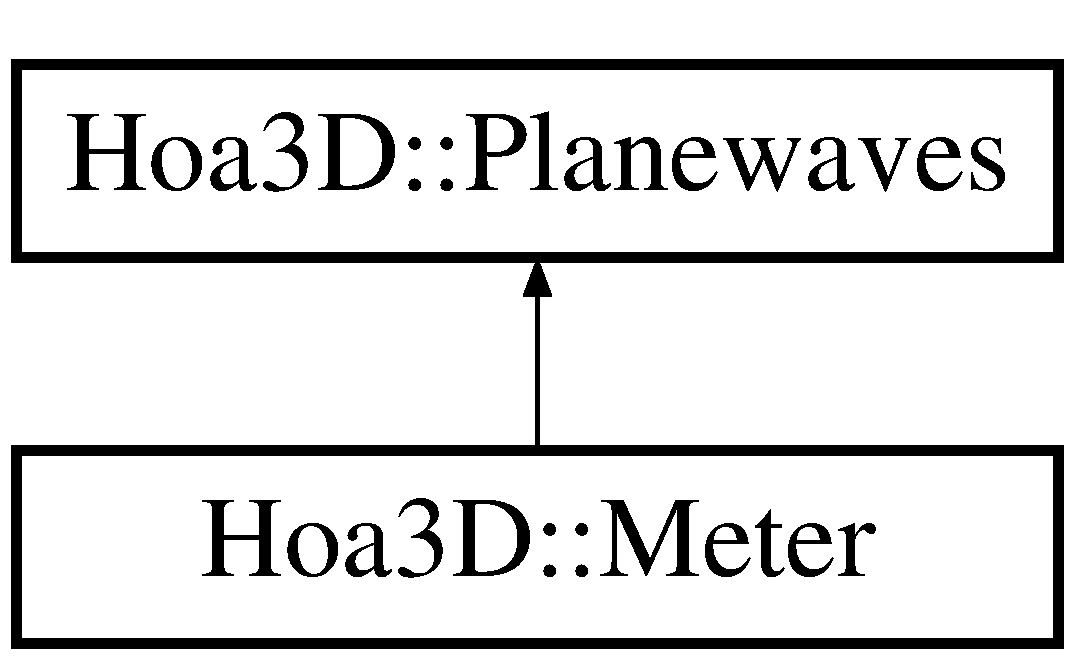
\includegraphics[height=2.000000cm]{class_hoa3_d_1_1_meter}
\end{center}
\end{figure}
\subsection*{Public Member Functions}
\begin{DoxyCompactItemize}
\item 
\hyperlink{class_hoa3_d_1_1_meter_a8dbe4a3655161c329540557cfed8c52a}{Meter} (unsigned int number\-Of\-Channels)
\begin{DoxyCompactList}\small\item\em The \hyperlink{class_hoa3_d_1_1_meter}{Meter} constructor. \end{DoxyCompactList}\item 
\hyperlink{class_hoa3_d_1_1_meter_a2f4d18e0007e96c1cd60e2f17d9575cc}{$\sim$\-Meter} ()
\begin{DoxyCompactList}\small\item\em The \hyperlink{class_hoa3_d_1_1_meter}{Meter} destructor. \end{DoxyCompactList}\item 
void \hyperlink{class_hoa3_d_1_1_meter_a85c538e8cf9791674a9ac6e602463dd0}{process} (const float $\ast$inputs)
\begin{DoxyCompactList}\small\item\em This method performs the widening with single precision. \end{DoxyCompactList}\item 
void \hyperlink{class_hoa3_d_1_1_meter_a273685843e1059b74b6d386dfb19c53b}{process} (const double $\ast$inputs)
\begin{DoxyCompactList}\small\item\em This method performs the widening with double precision. \end{DoxyCompactList}\end{DoxyCompactItemize}


\subsection{Detailed Description}
The ambisonic \hyperlink{class_hoa3_d_1_1_meter}{Meter}. 

The \hyperlink{class_hoa3_d_1_1_meter}{Meter} should be used to widen the sound propagation. 

Definition at line 17 of file Meter.\-h.



\subsection{Constructor \& Destructor Documentation}
\hypertarget{class_hoa3_d_1_1_meter_a8dbe4a3655161c329540557cfed8c52a}{\index{Hoa3\-D\-::\-Meter@{Hoa3\-D\-::\-Meter}!Meter@{Meter}}
\index{Meter@{Meter}!Hoa3D::Meter@{Hoa3\-D\-::\-Meter}}
\subsubsection[{Meter}]{\setlength{\rightskip}{0pt plus 5cm}Hoa3\-D\-::\-Meter\-::\-Meter (
\begin{DoxyParamCaption}
\item[{unsigned int}]{number\-Of\-Channels}
\end{DoxyParamCaption}
)}}\label{class_hoa3_d_1_1_meter_a8dbe4a3655161c329540557cfed8c52a}


The \hyperlink{class_hoa3_d_1_1_meter}{Meter} constructor. 

The \hyperlink{class_hoa3_d_1_1_meter}{Meter} constructor allocates and initialize the member values to computes spherical harmonics weighted coefficients depending of a decomposition order. The order must be at least 1.


\begin{DoxyParams}{Parameters}
{\em order} & The order. \\
\hline
\end{DoxyParams}


Definition at line 11 of file Meter.\-cpp.

\hypertarget{class_hoa3_d_1_1_meter_a2f4d18e0007e96c1cd60e2f17d9575cc}{\index{Hoa3\-D\-::\-Meter@{Hoa3\-D\-::\-Meter}!$\sim$\-Meter@{$\sim$\-Meter}}
\index{$\sim$\-Meter@{$\sim$\-Meter}!Hoa3D::Meter@{Hoa3\-D\-::\-Meter}}
\subsubsection[{$\sim$\-Meter}]{\setlength{\rightskip}{0pt plus 5cm}Hoa3\-D\-::\-Meter\-::$\sim$\-Meter (
\begin{DoxyParamCaption}
{}
\end{DoxyParamCaption}
)}}\label{class_hoa3_d_1_1_meter_a2f4d18e0007e96c1cd60e2f17d9575cc}


The \hyperlink{class_hoa3_d_1_1_meter}{Meter} destructor. 

The \hyperlink{class_hoa3_d_1_1_meter}{Meter} destructor free the memory. 

Definition at line 24 of file Meter.\-cpp.



\subsection{Member Function Documentation}
\hypertarget{class_hoa3_d_1_1_meter_a85c538e8cf9791674a9ac6e602463dd0}{\index{Hoa3\-D\-::\-Meter@{Hoa3\-D\-::\-Meter}!process@{process}}
\index{process@{process}!Hoa3D::Meter@{Hoa3\-D\-::\-Meter}}
\subsubsection[{process}]{\setlength{\rightskip}{0pt plus 5cm}void Hoa3\-D\-::\-Meter\-::process (
\begin{DoxyParamCaption}
\item[{const float $\ast$}]{inputs}
\end{DoxyParamCaption}
)}}\label{class_hoa3_d_1_1_meter_a85c538e8cf9791674a9ac6e602463dd0}


This method performs the widening with single precision. 

You should use this method for in-\/place or not-\/in-\/place processing and performs the widening sample by sample. The inputs array and outputs array contains the spherical harmonics samples and the minimum size must be the number of harmonics.


\begin{DoxyParams}{Parameters}
{\em inputs} & The input array. \\
\hline
\end{DoxyParams}


Definition at line 16 of file Meter.\-cpp.

\hypertarget{class_hoa3_d_1_1_meter_a273685843e1059b74b6d386dfb19c53b}{\index{Hoa3\-D\-::\-Meter@{Hoa3\-D\-::\-Meter}!process@{process}}
\index{process@{process}!Hoa3D::Meter@{Hoa3\-D\-::\-Meter}}
\subsubsection[{process}]{\setlength{\rightskip}{0pt plus 5cm}void Hoa3\-D\-::\-Meter\-::process (
\begin{DoxyParamCaption}
\item[{const double $\ast$}]{inputs}
\end{DoxyParamCaption}
)}}\label{class_hoa3_d_1_1_meter_a273685843e1059b74b6d386dfb19c53b}


This method performs the widening with double precision. 

You should use this method for in-\/place or not-\/in-\/place processing and performs the widening sample by sample. The inputs array and outputs array contains the spherical harmonics samples and the minimum size must be the number of harmonics.


\begin{DoxyParams}{Parameters}
{\em inputs} & The input array. \\
\hline
\end{DoxyParams}


Definition at line 20 of file Meter.\-cpp.



The documentation for this class was generated from the following files\-:\begin{DoxyCompactItemize}
\item 
/\-Users/\-Pierre/\-Source\-Tree/\-Hoa\-Library/\-Sources/\-Hoa3\-D/Meter.\-h\item 
/\-Users/\-Pierre/\-Source\-Tree/\-Hoa\-Library/\-Sources/\-Hoa3\-D/Meter.\-cpp\end{DoxyCompactItemize}

\hypertarget{class_hoa2_d_1_1_meter}{\section{Hoa2\-D\-:\-:Meter Class Reference}
\label{class_hoa2_d_1_1_meter}\index{Hoa2\-D\-::\-Meter@{Hoa2\-D\-::\-Meter}}
}


The planewaves peak level meter.  




{\ttfamily \#include $<$Meter.\-h$>$}

Inheritance diagram for Hoa2\-D\-:\-:Meter\-:\begin{figure}[H]
\begin{center}
\leavevmode
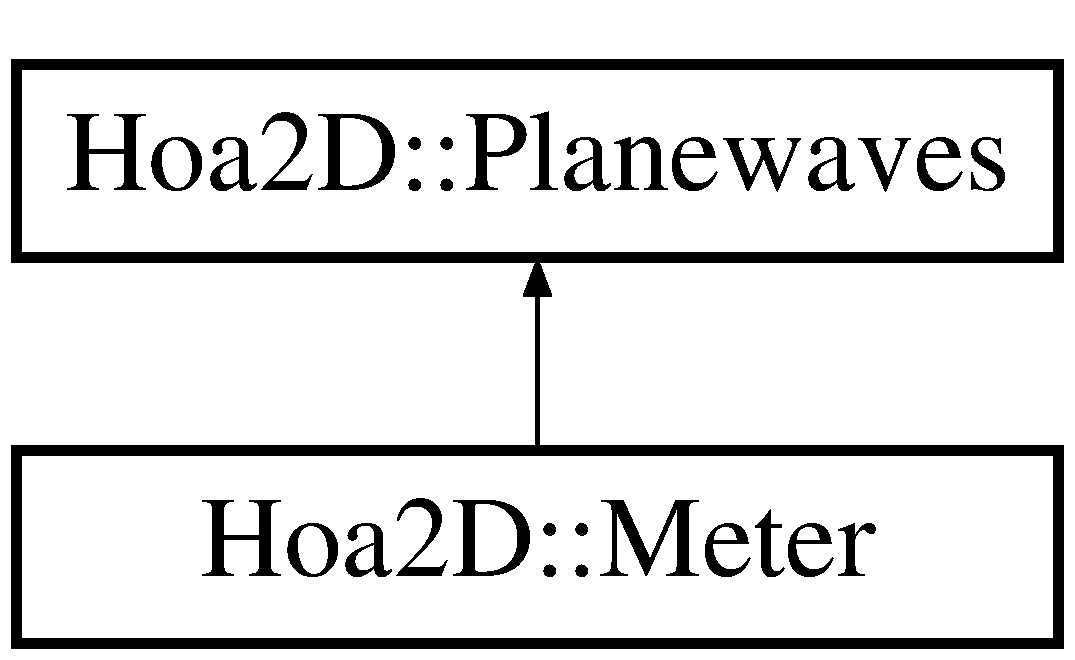
\includegraphics[height=2.000000cm]{class_hoa2_d_1_1_meter}
\end{center}
\end{figure}
\subsection*{Public Member Functions}
\begin{DoxyCompactItemize}
\item 
\hyperlink{class_hoa2_d_1_1_meter_a14d0584c4d3cd7fbfcbe73b7f9b072ce}{Meter} (unsigned int number\-Of\-Channels)
\begin{DoxyCompactList}\small\item\em The meter constructor. \end{DoxyCompactList}\item 
\hyperlink{class_hoa2_d_1_1_meter_a48276da266f600f4d24db748ff4ca046}{$\sim$\-Meter} ()
\begin{DoxyCompactList}\small\item\em The meter destructor. \end{DoxyCompactList}\item 
void \hyperlink{class_hoa2_d_1_1_meter_a6d6b2cbadbd05f9e731e22cd747f3008}{set\-Channel\-Position} (unsigned int index, double azimuth)
\begin{DoxyCompactList}\small\item\em Set the position of a loudspeaker. \end{DoxyCompactList}\item 
void \hyperlink{class_hoa2_d_1_1_meter_a1b05d443d17a910e7e9cc7b3f81badc6}{process} (const float $\ast$inputs)
\begin{DoxyCompactList}\small\item\em This method performs the widening with single precision. \end{DoxyCompactList}\item 
void \hyperlink{class_hoa2_d_1_1_meter_af523ed430333d4b861b117bda0bc6068}{process} (const double $\ast$inputs)
\begin{DoxyCompactList}\small\item\em This method performs the widening with double precision. \end{DoxyCompactList}\end{DoxyCompactItemize}
\subsection*{Additional Inherited Members}


\subsection{Detailed Description}
The planewaves peak level meter. 

The meter should be used to widen the sound propagation. 

Definition at line 18 of file Meter.\-h.



\subsection{Constructor \& Destructor Documentation}
\hypertarget{class_hoa2_d_1_1_meter_a14d0584c4d3cd7fbfcbe73b7f9b072ce}{\index{Hoa2\-D\-::\-Meter@{Hoa2\-D\-::\-Meter}!Meter@{Meter}}
\index{Meter@{Meter}!Hoa2D::Meter@{Hoa2\-D\-::\-Meter}}
\subsubsection[{Meter}]{\setlength{\rightskip}{0pt plus 5cm}Hoa2\-D\-::\-Meter\-::\-Meter (
\begin{DoxyParamCaption}
\item[{unsigned int}]{number\-Of\-Channels}
\end{DoxyParamCaption}
)}}\label{class_hoa2_d_1_1_meter_a14d0584c4d3cd7fbfcbe73b7f9b072ce}


The meter constructor. 

\begin{DoxyVerb}The meter constructor allocates and initialize the member values to computes spherical harmonics weighted coefficients depending of a decomposition order. The order must be at least 1.
\end{DoxyVerb}



\begin{DoxyParams}{Parameters}
{\em order} & The order. \\
\hline
\end{DoxyParams}


Definition at line 11 of file Meter.\-cpp.

\hypertarget{class_hoa2_d_1_1_meter_a48276da266f600f4d24db748ff4ca046}{\index{Hoa2\-D\-::\-Meter@{Hoa2\-D\-::\-Meter}!$\sim$\-Meter@{$\sim$\-Meter}}
\index{$\sim$\-Meter@{$\sim$\-Meter}!Hoa2D::Meter@{Hoa2\-D\-::\-Meter}}
\subsubsection[{$\sim$\-Meter}]{\setlength{\rightskip}{0pt plus 5cm}Hoa2\-D\-::\-Meter\-::$\sim$\-Meter (
\begin{DoxyParamCaption}
{}
\end{DoxyParamCaption}
)}}\label{class_hoa2_d_1_1_meter_a48276da266f600f4d24db748ff4ca046}


The meter destructor. 

The meter destructor free the memory. 

Definition at line 94 of file Meter.\-cpp.



\subsection{Member Function Documentation}
\hypertarget{class_hoa2_d_1_1_meter_a1b05d443d17a910e7e9cc7b3f81badc6}{\index{Hoa2\-D\-::\-Meter@{Hoa2\-D\-::\-Meter}!process@{process}}
\index{process@{process}!Hoa2D::Meter@{Hoa2\-D\-::\-Meter}}
\subsubsection[{process}]{\setlength{\rightskip}{0pt plus 5cm}void Hoa2\-D\-::\-Meter\-::process (
\begin{DoxyParamCaption}
\item[{const float $\ast$}]{inputs}
\end{DoxyParamCaption}
)}}\label{class_hoa2_d_1_1_meter_a1b05d443d17a910e7e9cc7b3f81badc6}


This method performs the widening with single precision. 

You should use this method for in-\/place or not-\/in-\/place processing and performs the widening sample by sample. The inputs array and outputs array contains the spherical harmonics samples and the minimum size must be the number of harmonics.


\begin{DoxyParams}{Parameters}
{\em inputs} & The inputs array. \\
\hline
\end{DoxyParams}


Definition at line 54 of file Meter.\-cpp.

\hypertarget{class_hoa2_d_1_1_meter_af523ed430333d4b861b117bda0bc6068}{\index{Hoa2\-D\-::\-Meter@{Hoa2\-D\-::\-Meter}!process@{process}}
\index{process@{process}!Hoa2D::Meter@{Hoa2\-D\-::\-Meter}}
\subsubsection[{process}]{\setlength{\rightskip}{0pt plus 5cm}void Hoa2\-D\-::\-Meter\-::process (
\begin{DoxyParamCaption}
\item[{const double $\ast$}]{inputs}
\end{DoxyParamCaption}
)}}\label{class_hoa2_d_1_1_meter_af523ed430333d4b861b117bda0bc6068}


This method performs the widening with double precision. 

You should use this method for in-\/place or not-\/in-\/place processing and performs the widening sample by sample. The inputs array and outputs array contains the spherical harmonics samples and the minimum size must be the number of harmonics.


\begin{DoxyParams}{Parameters}
{\em inputs} & The inputs array. \\
\hline
\end{DoxyParams}


Definition at line 74 of file Meter.\-cpp.

\hypertarget{class_hoa2_d_1_1_meter_a6d6b2cbadbd05f9e731e22cd747f3008}{\index{Hoa2\-D\-::\-Meter@{Hoa2\-D\-::\-Meter}!set\-Channel\-Position@{set\-Channel\-Position}}
\index{set\-Channel\-Position@{set\-Channel\-Position}!Hoa2D::Meter@{Hoa2\-D\-::\-Meter}}
\subsubsection[{set\-Channel\-Position}]{\setlength{\rightskip}{0pt plus 5cm}void Hoa2\-D\-::\-Meter\-::set\-Channel\-Position (
\begin{DoxyParamCaption}
\item[{unsigned int}]{index, }
\item[{double}]{azimuth}
\end{DoxyParamCaption}
)}}\label{class_hoa2_d_1_1_meter_a6d6b2cbadbd05f9e731e22cd747f3008}


Set the position of a loudspeaker. 

Set the position of a loudspeaker with polar coordinates. The azimtuh is in radian between 0 and 2 Pi, O is the front of the soundfield and Pi is the back of the sound field. The elevation is in radian between -\/1/2 Pi and 1/2 Pi, -\/1/2 Pi the the bottom of the sound field, 0 is the center of the sound field and 1/2 Pi is the top of the sound field. The maximum index must be the number of loudspeakers -\/ 1.


\begin{DoxyParams}{Parameters}
{\em index} & The index of the loudspeaker. \\
\hline
{\em azimuth} & The azimuth. \\
\hline
{\em elevation} & The elevation. \\
\hline
\end{DoxyParams}


Definition at line 24 of file Meter.\-cpp.



The documentation for this class was generated from the following files\-:\begin{DoxyCompactItemize}
\item 
/\-Users/elioton/\-Documents/programmation/\-C\-I\-C\-M/source\-Tree/\-Hoa\-Library/\-Sources/\-Hoa2\-D/Meter.\-h\item 
/\-Users/elioton/\-Documents/programmation/\-C\-I\-C\-M/source\-Tree/\-Hoa\-Library/\-Sources/\-Hoa2\-D/Meter.\-cpp\end{DoxyCompactItemize}

\hypertarget{class_hoa3_d_1_1_optim}{\section{Hoa3\-D\-:\-:Optim Class Reference}
\label{class_hoa3_d_1_1_optim}\index{Hoa3\-D\-::\-Optim@{Hoa3\-D\-::\-Optim}}
}


The ambisonic optimization.  




{\ttfamily \#include $<$Optim.\-h$>$}

Inheritance diagram for Hoa3\-D\-:\-:Optim\-:\begin{figure}[H]
\begin{center}
\leavevmode
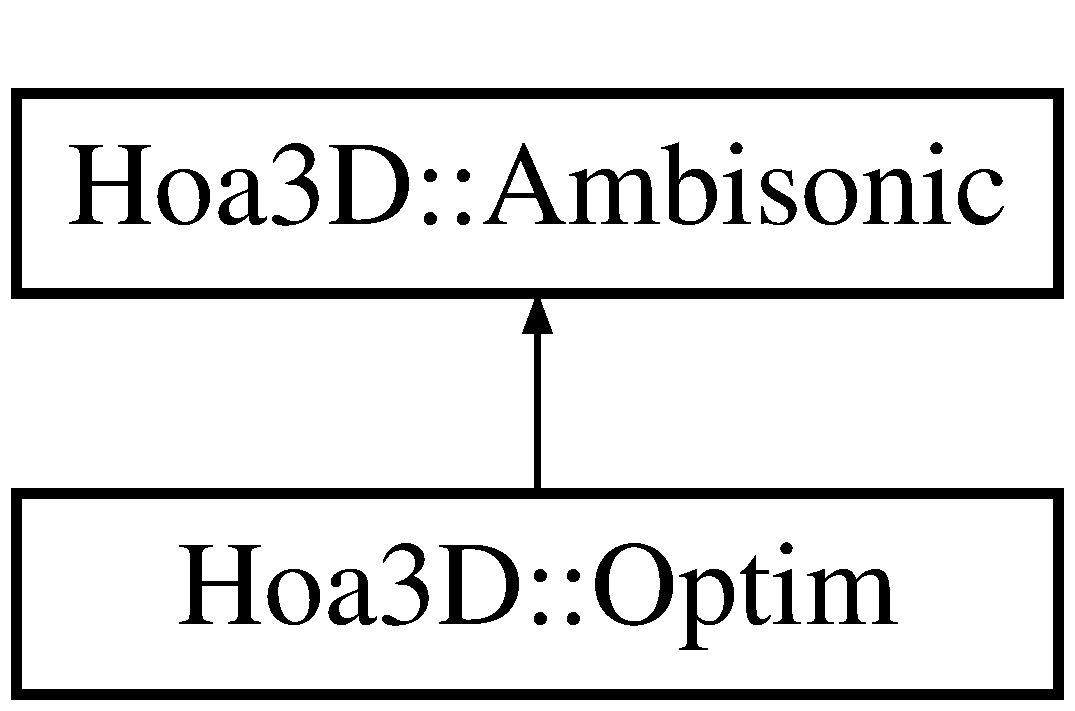
\includegraphics[height=2.000000cm]{class_hoa3_d_1_1_optim}
\end{center}
\end{figure}
\subsection*{Public Types}
\begin{DoxyCompactItemize}
\item 
enum \hyperlink{class_hoa3_d_1_1_optim_a1a153ac21e7a112279824f17981cf147}{Mode} \{ \hyperlink{class_hoa3_d_1_1_optim_a1a153ac21e7a112279824f17981cf147a89acb58975922396713cc88cafc55b45}{Basic} = 0, 
\hyperlink{class_hoa3_d_1_1_optim_a1a153ac21e7a112279824f17981cf147a491a405ba48de3977668d54a8d9ff44a}{Max\-Re} = 1, 
\hyperlink{class_hoa3_d_1_1_optim_a1a153ac21e7a112279824f17981cf147a55da4ad4519ee8860e9ea45cc475241c}{In\-Phase} = 2
 \}
\end{DoxyCompactItemize}
\subsection*{Public Member Functions}
\begin{DoxyCompactItemize}
\item 
\hyperlink{class_hoa3_d_1_1_optim_ab53ffe61910a75637afafb7f4f3ba788}{Optim} (unsigned int order, \hyperlink{class_hoa3_d_1_1_optim_a1a153ac21e7a112279824f17981cf147}{Mode} mode)
\begin{DoxyCompactList}\small\item\em The optimization constructor. \end{DoxyCompactList}\item 
\hyperlink{class_hoa3_d_1_1_optim_a11c05a8b458f79ba09f4eefad63e0b20}{$\sim$\-Optim} ()
\begin{DoxyCompactList}\small\item\em The optimization destructor. \end{DoxyCompactList}\item 
void \hyperlink{class_hoa3_d_1_1_optim_abb49c9e6a327bc62ac6491cd3046a10a}{set\-Mode} (\hyperlink{class_hoa3_d_1_1_optim_a1a153ac21e7a112279824f17981cf147}{Mode} mode)
\begin{DoxyCompactList}\small\item\em This method set the optimization mode. \end{DoxyCompactList}\item 
\hyperlink{class_hoa3_d_1_1_optim_a1a153ac21e7a112279824f17981cf147}{Mode} \hyperlink{class_hoa3_d_1_1_optim_a0446c68d06a5fd112f3e608c82d69b7f}{get\-Mode} () const 
\begin{DoxyCompactList}\small\item\em Retrieve the optimization mode. \end{DoxyCompactList}\item 
void \hyperlink{class_hoa3_d_1_1_optim_a13f8cb746e5bcc3c096bd0c0bf1a6435}{process} (const float $\ast$inputs, float $\ast$outputs)
\begin{DoxyCompactList}\small\item\em This method performs the optimization with single precision. \end{DoxyCompactList}\item 
void \hyperlink{class_hoa3_d_1_1_optim_a6c2e7ce20ec5f98e9e609040144ea99d}{process} (const double $\ast$inputs, double $\ast$outputs)
\begin{DoxyCompactList}\small\item\em This method performs the optimization with double precision. \end{DoxyCompactList}\end{DoxyCompactItemize}


\subsection{Detailed Description}
The ambisonic optimization. 

The optimization should be used to optimize the ambisonic sound field. There are 3 optimization modes, Basic (no optimizations), Max\-Re (energy vector optimization) and In\-Phase (energy and velocity vector optimization). Basic has no effect, it should be used with a perfect ambisonic loudspeakers (arrengement where all the loudspeakers are to equal distance on a sphere) and for a listener placed at the perfect center of the sphere. Max\-Re should be used for auditory confined to the center of the sphere. In\-Phase should be used when the auditory covers the entire loudspeaker area and when the loudspeakers arragement is not a perfect sphere or when the loudspeakers are not to equal distance. Note that the optimizations decrease the precision sound field restitution thus it can be compared to particular cases of the fractional orders. 

Definition at line 17 of file Optim.\-h.



\subsection{Member Enumeration Documentation}
\hypertarget{class_hoa3_d_1_1_optim_a1a153ac21e7a112279824f17981cf147}{\index{Hoa3\-D\-::\-Optim@{Hoa3\-D\-::\-Optim}!Mode@{Mode}}
\index{Mode@{Mode}!Hoa3D::Optim@{Hoa3\-D\-::\-Optim}}
\subsubsection[{Mode}]{\setlength{\rightskip}{0pt plus 5cm}enum {\bf Hoa3\-D\-::\-Optim\-::\-Mode}}}\label{class_hoa3_d_1_1_optim_a1a153ac21e7a112279824f17981cf147}
\begin{Desc}
\item[Enumerator]\par
\begin{description}
\index{Basic@{Basic}!Hoa3\-D\-::\-Optim@{Hoa3\-D\-::\-Optim}}\index{Hoa3\-D\-::\-Optim@{Hoa3\-D\-::\-Optim}!Basic@{Basic}}\item[{\em 
\hypertarget{class_hoa3_d_1_1_optim_a1a153ac21e7a112279824f17981cf147a89acb58975922396713cc88cafc55b45}{Basic}\label{class_hoa3_d_1_1_optim_a1a153ac21e7a112279824f17981cf147a89acb58975922396713cc88cafc55b45}
}]basic Optimization \index{Max\-Re@{Max\-Re}!Hoa3\-D\-::\-Optim@{Hoa3\-D\-::\-Optim}}\index{Hoa3\-D\-::\-Optim@{Hoa3\-D\-::\-Optim}!Max\-Re@{Max\-Re}}\item[{\em 
\hypertarget{class_hoa3_d_1_1_optim_a1a153ac21e7a112279824f17981cf147a491a405ba48de3977668d54a8d9ff44a}{Max\-Re}\label{class_hoa3_d_1_1_optim_a1a153ac21e7a112279824f17981cf147a491a405ba48de3977668d54a8d9ff44a}
}]max-\/re Optimization \index{In\-Phase@{In\-Phase}!Hoa3\-D\-::\-Optim@{Hoa3\-D\-::\-Optim}}\index{Hoa3\-D\-::\-Optim@{Hoa3\-D\-::\-Optim}!In\-Phase@{In\-Phase}}\item[{\em 
\hypertarget{class_hoa3_d_1_1_optim_a1a153ac21e7a112279824f17981cf147a55da4ad4519ee8860e9ea45cc475241c}{In\-Phase}\label{class_hoa3_d_1_1_optim_a1a153ac21e7a112279824f17981cf147a55da4ad4519ee8860e9ea45cc475241c}
}]in-\/phase Optimization \end{description}
\end{Desc}


Definition at line 20 of file Optim.\-h.



\subsection{Constructor \& Destructor Documentation}
\hypertarget{class_hoa3_d_1_1_optim_ab53ffe61910a75637afafb7f4f3ba788}{\index{Hoa3\-D\-::\-Optim@{Hoa3\-D\-::\-Optim}!Optim@{Optim}}
\index{Optim@{Optim}!Hoa3D::Optim@{Hoa3\-D\-::\-Optim}}
\subsubsection[{Optim}]{\setlength{\rightskip}{0pt plus 5cm}Hoa3\-D\-::\-Optim\-::\-Optim (
\begin{DoxyParamCaption}
\item[{unsigned int}]{order, }
\item[{{\bf Mode}}]{mode}
\end{DoxyParamCaption}
)}}\label{class_hoa3_d_1_1_optim_ab53ffe61910a75637afafb7f4f3ba788}


The optimization constructor. 

The optimization constructor allocates and initialize the member values to computes spherical harmonics weighted coefficients depending of a decomposition order. The order must be at least 1.


\begin{DoxyParams}{Parameters}
{\em order} & The order. \\
\hline
{\em mode} & The optimization mode. \\
\hline
\end{DoxyParams}


Definition at line 11 of file Optim.\-cpp.

\hypertarget{class_hoa3_d_1_1_optim_a11c05a8b458f79ba09f4eefad63e0b20}{\index{Hoa3\-D\-::\-Optim@{Hoa3\-D\-::\-Optim}!$\sim$\-Optim@{$\sim$\-Optim}}
\index{$\sim$\-Optim@{$\sim$\-Optim}!Hoa3D::Optim@{Hoa3\-D\-::\-Optim}}
\subsubsection[{$\sim$\-Optim}]{\setlength{\rightskip}{0pt plus 5cm}Hoa3\-D\-::\-Optim\-::$\sim$\-Optim (
\begin{DoxyParamCaption}
{}
\end{DoxyParamCaption}
)}}\label{class_hoa3_d_1_1_optim_a11c05a8b458f79ba09f4eefad63e0b20}


The optimization destructor. 

The optimization destructor free the memory. 

Definition at line 57 of file Optim.\-cpp.



\subsection{Member Function Documentation}
\hypertarget{class_hoa3_d_1_1_optim_a0446c68d06a5fd112f3e608c82d69b7f}{\index{Hoa3\-D\-::\-Optim@{Hoa3\-D\-::\-Optim}!get\-Mode@{get\-Mode}}
\index{get\-Mode@{get\-Mode}!Hoa3D::Optim@{Hoa3\-D\-::\-Optim}}
\subsubsection[{get\-Mode}]{\setlength{\rightskip}{0pt plus 5cm}{\bf Mode} Hoa3\-D\-::\-Optim\-::get\-Mode (
\begin{DoxyParamCaption}
{}
\end{DoxyParamCaption}
) const\hspace{0.3cm}{\ttfamily [inline]}}}\label{class_hoa3_d_1_1_optim_a0446c68d06a5fd112f3e608c82d69b7f}


Retrieve the optimization mode. 

Retrieve the optimization mode \-: Basic, Max\-Re or In\-Phase.

\begin{DoxyReturn}{Returns}
The method returns the optimization mode. 
\end{DoxyReturn}


Definition at line 59 of file Optim.\-h.

\hypertarget{class_hoa3_d_1_1_optim_a13f8cb746e5bcc3c096bd0c0bf1a6435}{\index{Hoa3\-D\-::\-Optim@{Hoa3\-D\-::\-Optim}!process@{process}}
\index{process@{process}!Hoa3D::Optim@{Hoa3\-D\-::\-Optim}}
\subsubsection[{process}]{\setlength{\rightskip}{0pt plus 5cm}void Hoa3\-D\-::\-Optim\-::process (
\begin{DoxyParamCaption}
\item[{const float $\ast$}]{inputs, }
\item[{float $\ast$}]{outputs}
\end{DoxyParamCaption}
)}}\label{class_hoa3_d_1_1_optim_a13f8cb746e5bcc3c096bd0c0bf1a6435}


This method performs the optimization with single precision. 

You should use this method for in-\/place or not-\/in-\/place processing and performs the optimization sample by sample. The inputs array and outputs array contains the spherical harmonics samples and the minimum size must be the number of harmonics.


\begin{DoxyParams}{Parameters}
{\em inputs} & The input array. \\
\hline
{\em outputs} & The output array. \\
\hline
\end{DoxyParams}


Definition at line 45 of file Optim.\-cpp.

\hypertarget{class_hoa3_d_1_1_optim_a6c2e7ce20ec5f98e9e609040144ea99d}{\index{Hoa3\-D\-::\-Optim@{Hoa3\-D\-::\-Optim}!process@{process}}
\index{process@{process}!Hoa3D::Optim@{Hoa3\-D\-::\-Optim}}
\subsubsection[{process}]{\setlength{\rightskip}{0pt plus 5cm}void Hoa3\-D\-::\-Optim\-::process (
\begin{DoxyParamCaption}
\item[{const double $\ast$}]{inputs, }
\item[{double $\ast$}]{outputs}
\end{DoxyParamCaption}
)}}\label{class_hoa3_d_1_1_optim_a6c2e7ce20ec5f98e9e609040144ea99d}


This method performs the optimization with double precision. 

You should use this method for in-\/place or not-\/in-\/place processing and performs the optimization sample by sample. The inputs array and outputs array contains the spherical harmonics samples and the minimum size must be the number of harmonics.


\begin{DoxyParams}{Parameters}
{\em inputs} & The input array. \\
\hline
{\em outputs} & The output array. \\
\hline
\end{DoxyParams}


Definition at line 51 of file Optim.\-cpp.

\hypertarget{class_hoa3_d_1_1_optim_abb49c9e6a327bc62ac6491cd3046a10a}{\index{Hoa3\-D\-::\-Optim@{Hoa3\-D\-::\-Optim}!set\-Mode@{set\-Mode}}
\index{set\-Mode@{set\-Mode}!Hoa3D::Optim@{Hoa3\-D\-::\-Optim}}
\subsubsection[{set\-Mode}]{\setlength{\rightskip}{0pt plus 5cm}void Hoa3\-D\-::\-Optim\-::set\-Mode (
\begin{DoxyParamCaption}
\item[{{\bf Mode}}]{mode}
\end{DoxyParamCaption}
)}}\label{class_hoa3_d_1_1_optim_abb49c9e6a327bc62ac6491cd3046a10a}


This method set the optimization mode. 

The mode should be one of the 3 optimization modes, Basic, Max\-Re or In\-Phase.


\begin{DoxyParams}{Parameters}
{\em mode} & The optimization mode. \\
\hline
\end{DoxyParams}


Definition at line 17 of file Optim.\-cpp.



The documentation for this class was generated from the following files\-:\begin{DoxyCompactItemize}
\item 
/\-Users/\-Pierre/\-Source\-Tree/\-Hoa\-Library/\-Sources/\-Hoa3\-D/Optim.\-h\item 
/\-Users/\-Pierre/\-Source\-Tree/\-Hoa\-Library/\-Sources/\-Hoa3\-D/Optim.\-cpp\end{DoxyCompactItemize}

\hypertarget{class_hoa2_d_1_1_optim}{\section{Hoa2\-D\-:\-:Optim Class Reference}
\label{class_hoa2_d_1_1_optim}\index{Hoa2\-D\-::\-Optim@{Hoa2\-D\-::\-Optim}}
}


The ambisonic optimization.  




{\ttfamily \#include $<$Optim.\-h$>$}

Inheritance diagram for Hoa2\-D\-:\-:Optim\-:\begin{figure}[H]
\begin{center}
\leavevmode
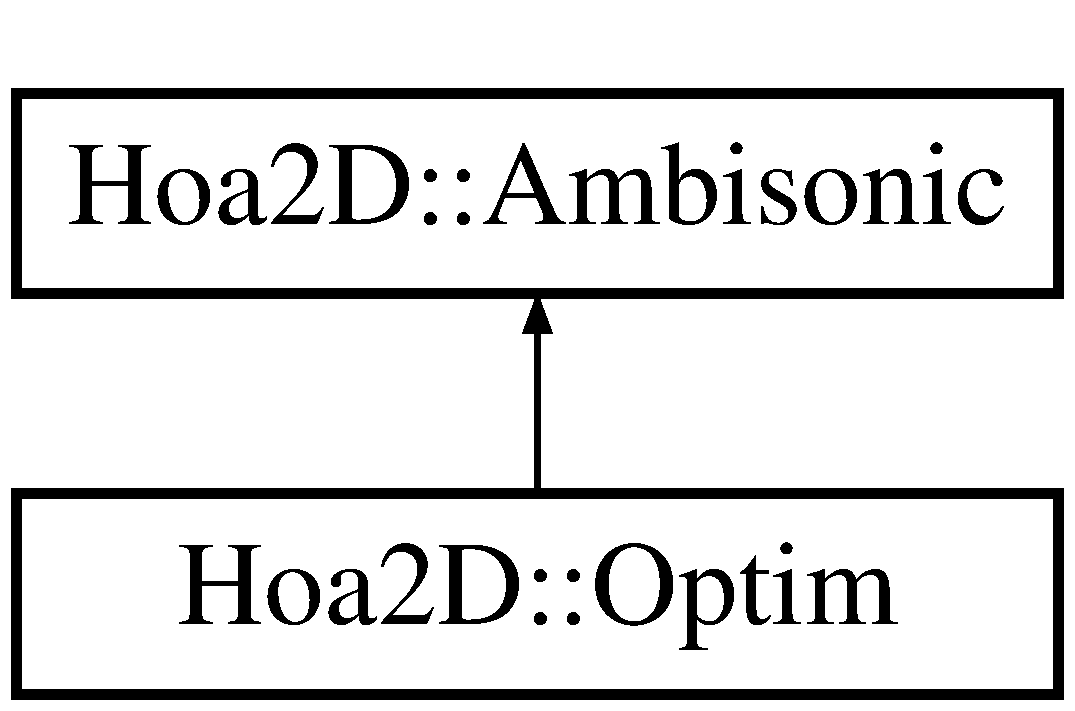
\includegraphics[height=2.000000cm]{class_hoa2_d_1_1_optim}
\end{center}
\end{figure}
\subsection*{Public Types}
\begin{DoxyCompactItemize}
\item 
enum \hyperlink{class_hoa2_d_1_1_optim_ae40f22368cb55699cf19729e37c0aff3}{Mode} \{ \hyperlink{class_hoa2_d_1_1_optim_ae40f22368cb55699cf19729e37c0aff3af5bbb98a42968855f2f43d9a708ae8d2}{Basic} = 0, 
\hyperlink{class_hoa2_d_1_1_optim_ae40f22368cb55699cf19729e37c0aff3a6b8b2446e2cffae18f5f4625b68e0f21}{Max\-Re} = 1, 
\hyperlink{class_hoa2_d_1_1_optim_ae40f22368cb55699cf19729e37c0aff3aa9a64070fdf166180add5ac7a8e24567}{In\-Phase} = 2
 \}
\end{DoxyCompactItemize}
\subsection*{Public Member Functions}
\begin{DoxyCompactItemize}
\item 
\hyperlink{class_hoa2_d_1_1_optim_a5e11da74b3e87ad15db6538d31eb3628}{Optim} (unsigned int order, \hyperlink{class_hoa2_d_1_1_optim_ae40f22368cb55699cf19729e37c0aff3}{Mode} mode)
\begin{DoxyCompactList}\small\item\em The optimization constructor. \end{DoxyCompactList}\item 
\hyperlink{class_hoa2_d_1_1_optim_a71b6d88873b054944db6efd2713bf8d3}{$\sim$\-Optim} ()
\begin{DoxyCompactList}\small\item\em The optimization destructor. \end{DoxyCompactList}\item 
\hyperlink{class_hoa2_d_1_1_optim_ae40f22368cb55699cf19729e37c0aff3}{Mode} \hyperlink{class_hoa2_d_1_1_optim_ab75c7150c5918ed05219212b426aa04b}{get\-Mode} () const 
\begin{DoxyCompactList}\small\item\em Retrieve the optimization mode. \end{DoxyCompactList}\item 
void \hyperlink{class_hoa2_d_1_1_optim_a2ea2227817c133aeaf2732880d8214ce}{set\-Mode} (\hyperlink{class_hoa2_d_1_1_optim_ae40f22368cb55699cf19729e37c0aff3}{Mode} mode)
\begin{DoxyCompactList}\small\item\em This method set the optimization mode. \end{DoxyCompactList}\item 
void \hyperlink{class_hoa2_d_1_1_optim_afca15242cbca4fefe08c6f17d2b42241}{process} (const float $\ast$inputs, float $\ast$outputs)
\begin{DoxyCompactList}\small\item\em This method performs the optimization with single precision. \end{DoxyCompactList}\item 
void \hyperlink{class_hoa2_d_1_1_optim_ac0c905a79204c921568952c787376120}{process} (const double $\ast$inputs, double $\ast$outputs)
\begin{DoxyCompactList}\small\item\em This method performs the optimization with double precision. \end{DoxyCompactList}\end{DoxyCompactItemize}


\subsection{Detailed Description}
The ambisonic optimization. 

The optimization should be used to optimize the ambisonic sound field. There are 3 optimization modes, Basic (no optimization), Max\-Re (energy vector optimization) and In\-Phase (energy and velocity vector optimization). Basic has no effect, it should be used with a perfect ambisonic loudspeakers, arrengement where all the loudspeakers are to equal distance on a circle, and for a listener placed at the perfect center of the circle. Max\-Re should be used for auditory confined to the center of the circle. In\-Phase should be used when the auditory covers the entire loudspeakers area and when the loudspeakers arragement is not a perfect circle or when the loudspeakers are not to equal distance. Note that the optimizations decrease the precision of the sound field restitution thus it can be compared to particular cases of the fractional orders. 

Definition at line 16 of file Optim.\-h.



\subsection{Member Enumeration Documentation}
\hypertarget{class_hoa2_d_1_1_optim_ae40f22368cb55699cf19729e37c0aff3}{\index{Hoa2\-D\-::\-Optim@{Hoa2\-D\-::\-Optim}!Mode@{Mode}}
\index{Mode@{Mode}!Hoa2D::Optim@{Hoa2\-D\-::\-Optim}}
\subsubsection[{Mode}]{\setlength{\rightskip}{0pt plus 5cm}enum {\bf Hoa2\-D\-::\-Optim\-::\-Mode}}}\label{class_hoa2_d_1_1_optim_ae40f22368cb55699cf19729e37c0aff3}
\begin{Desc}
\item[Enumerator]\par
\begin{description}
\index{Basic@{Basic}!Hoa2\-D\-::\-Optim@{Hoa2\-D\-::\-Optim}}\index{Hoa2\-D\-::\-Optim@{Hoa2\-D\-::\-Optim}!Basic@{Basic}}\item[{\em 
\hypertarget{class_hoa2_d_1_1_optim_ae40f22368cb55699cf19729e37c0aff3af5bbb98a42968855f2f43d9a708ae8d2}{Basic}\label{class_hoa2_d_1_1_optim_ae40f22368cb55699cf19729e37c0aff3af5bbb98a42968855f2f43d9a708ae8d2}
}]Basic Optimization \index{Max\-Re@{Max\-Re}!Hoa2\-D\-::\-Optim@{Hoa2\-D\-::\-Optim}}\index{Hoa2\-D\-::\-Optim@{Hoa2\-D\-::\-Optim}!Max\-Re@{Max\-Re}}\item[{\em 
\hypertarget{class_hoa2_d_1_1_optim_ae40f22368cb55699cf19729e37c0aff3a6b8b2446e2cffae18f5f4625b68e0f21}{Max\-Re}\label{class_hoa2_d_1_1_optim_ae40f22368cb55699cf19729e37c0aff3a6b8b2446e2cffae18f5f4625b68e0f21}
}]Max Re Optimization \index{In\-Phase@{In\-Phase}!Hoa2\-D\-::\-Optim@{Hoa2\-D\-::\-Optim}}\index{Hoa2\-D\-::\-Optim@{Hoa2\-D\-::\-Optim}!In\-Phase@{In\-Phase}}\item[{\em 
\hypertarget{class_hoa2_d_1_1_optim_ae40f22368cb55699cf19729e37c0aff3aa9a64070fdf166180add5ac7a8e24567}{In\-Phase}\label{class_hoa2_d_1_1_optim_ae40f22368cb55699cf19729e37c0aff3aa9a64070fdf166180add5ac7a8e24567}
}]In Phase Optimization \end{description}
\end{Desc}


Definition at line 19 of file Optim.\-h.



\subsection{Constructor \& Destructor Documentation}
\hypertarget{class_hoa2_d_1_1_optim_a5e11da74b3e87ad15db6538d31eb3628}{\index{Hoa2\-D\-::\-Optim@{Hoa2\-D\-::\-Optim}!Optim@{Optim}}
\index{Optim@{Optim}!Hoa2D::Optim@{Hoa2\-D\-::\-Optim}}
\subsubsection[{Optim}]{\setlength{\rightskip}{0pt plus 5cm}Hoa2\-D\-::\-Optim\-::\-Optim (
\begin{DoxyParamCaption}
\item[{unsigned int}]{order, }
\item[{{\bf Mode}}]{mode}
\end{DoxyParamCaption}
)}}\label{class_hoa2_d_1_1_optim_a5e11da74b3e87ad15db6538d31eb3628}


The optimization constructor. 

The optimization constructor allocates and initialize the member values to computes spherical harmonics weighted coefficients depending of a decomposition order. The order must be at least 1.


\begin{DoxyParams}{Parameters}
{\em order} & The order. \\
\hline
\end{DoxyParams}


Definition at line 11 of file Optim.\-cpp.

\hypertarget{class_hoa2_d_1_1_optim_a71b6d88873b054944db6efd2713bf8d3}{\index{Hoa2\-D\-::\-Optim@{Hoa2\-D\-::\-Optim}!$\sim$\-Optim@{$\sim$\-Optim}}
\index{$\sim$\-Optim@{$\sim$\-Optim}!Hoa2D::Optim@{Hoa2\-D\-::\-Optim}}
\subsubsection[{$\sim$\-Optim}]{\setlength{\rightskip}{0pt plus 5cm}Hoa2\-D\-::\-Optim\-::$\sim$\-Optim (
\begin{DoxyParamCaption}
{}
\end{DoxyParamCaption}
)}}\label{class_hoa2_d_1_1_optim_a71b6d88873b054944db6efd2713bf8d3}


The optimization destructor. 

The optimization destructor free the memory. 

Definition at line 59 of file Optim.\-cpp.



\subsection{Member Function Documentation}
\hypertarget{class_hoa2_d_1_1_optim_ab75c7150c5918ed05219212b426aa04b}{\index{Hoa2\-D\-::\-Optim@{Hoa2\-D\-::\-Optim}!get\-Mode@{get\-Mode}}
\index{get\-Mode@{get\-Mode}!Hoa2D::Optim@{Hoa2\-D\-::\-Optim}}
\subsubsection[{get\-Mode}]{\setlength{\rightskip}{0pt plus 5cm}{\bf Mode} Hoa2\-D\-::\-Optim\-::get\-Mode (
\begin{DoxyParamCaption}
{}
\end{DoxyParamCaption}
) const\hspace{0.3cm}{\ttfamily [inline]}}}\label{class_hoa2_d_1_1_optim_ab75c7150c5918ed05219212b426aa04b}


Retrieve the optimization mode. 

Retrieve the optimization mode \-: Basic, Max\-Re or In\-Phase.

\begin{DoxyReturn}{Returns}
The method returns the optimization mode. 
\end{DoxyReturn}


Definition at line 50 of file Optim.\-h.

\hypertarget{class_hoa2_d_1_1_optim_afca15242cbca4fefe08c6f17d2b42241}{\index{Hoa2\-D\-::\-Optim@{Hoa2\-D\-::\-Optim}!process@{process}}
\index{process@{process}!Hoa2D::Optim@{Hoa2\-D\-::\-Optim}}
\subsubsection[{process}]{\setlength{\rightskip}{0pt plus 5cm}void Hoa2\-D\-::\-Optim\-::process (
\begin{DoxyParamCaption}
\item[{const float $\ast$}]{inputs, }
\item[{float $\ast$}]{outputs}
\end{DoxyParamCaption}
)}}\label{class_hoa2_d_1_1_optim_afca15242cbca4fefe08c6f17d2b42241}


This method performs the optimization with single precision. 

You should use this method for in-\/place or not-\/in-\/place processing and performs the optimization sample by sample. The inputs array and outputs array contains the spherical harmonics samples and the minimum size must be the number of harmonics.


\begin{DoxyParams}{Parameters}
{\em inputs} & The inputs array. \\
\hline
{\em outputs} & The outputs array. \\
\hline
\end{DoxyParams}


Definition at line 47 of file Optim.\-cpp.

\hypertarget{class_hoa2_d_1_1_optim_ac0c905a79204c921568952c787376120}{\index{Hoa2\-D\-::\-Optim@{Hoa2\-D\-::\-Optim}!process@{process}}
\index{process@{process}!Hoa2D::Optim@{Hoa2\-D\-::\-Optim}}
\subsubsection[{process}]{\setlength{\rightskip}{0pt plus 5cm}void Hoa2\-D\-::\-Optim\-::process (
\begin{DoxyParamCaption}
\item[{const double $\ast$}]{inputs, }
\item[{double $\ast$}]{outputs}
\end{DoxyParamCaption}
)}}\label{class_hoa2_d_1_1_optim_ac0c905a79204c921568952c787376120}


This method performs the optimization with double precision. 

You should use this method for in-\/place or not-\/in-\/place processing and performs the optimization sample by sample. The inputs array and outputs array contains the spherical harmonics samples and the minimum size must be the number of harmonics.


\begin{DoxyParams}{Parameters}
{\em inputs} & The inputs array. \\
\hline
{\em outputs} & The outputs array. \\
\hline
\end{DoxyParams}


Definition at line 53 of file Optim.\-cpp.

\hypertarget{class_hoa2_d_1_1_optim_a2ea2227817c133aeaf2732880d8214ce}{\index{Hoa2\-D\-::\-Optim@{Hoa2\-D\-::\-Optim}!set\-Mode@{set\-Mode}}
\index{set\-Mode@{set\-Mode}!Hoa2D::Optim@{Hoa2\-D\-::\-Optim}}
\subsubsection[{set\-Mode}]{\setlength{\rightskip}{0pt plus 5cm}void Hoa2\-D\-::\-Optim\-::set\-Mode (
\begin{DoxyParamCaption}
\item[{{\bf Mode}}]{mode}
\end{DoxyParamCaption}
)}}\label{class_hoa2_d_1_1_optim_a2ea2227817c133aeaf2732880d8214ce}


This method set the optimization mode. 

The mode should be one of the 3 optimization modes, Basic, Max\-Re or In\-Phase.


\begin{DoxyParams}{Parameters}
{\em mode} & The optimization mode. \\
\hline
\end{DoxyParams}


Definition at line 17 of file Optim.\-cpp.



The documentation for this class was generated from the following files\-:\begin{DoxyCompactItemize}
\item 
/\-Users/\-Pierre/\-Source\-Tree/\-Hoa\-Library/\-Sources/\-Hoa2\-D/Optim.\-h\item 
/\-Users/\-Pierre/\-Source\-Tree/\-Hoa\-Library/\-Sources/\-Hoa2\-D/Optim.\-cpp\end{DoxyCompactItemize}

\hypertarget{class_hoa2_d_1_1_planewaves}{\section{Hoa2\-D\-:\-:Planewaves Class Reference}
\label{class_hoa2_d_1_1_planewaves}\index{Hoa2\-D\-::\-Planewaves@{Hoa2\-D\-::\-Planewaves}}
}


The planewaves class.  




{\ttfamily \#include $<$Planewaves.\-h$>$}

Inheritance diagram for Hoa2\-D\-:\-:Planewaves\-:\begin{figure}[H]
\begin{center}
\leavevmode
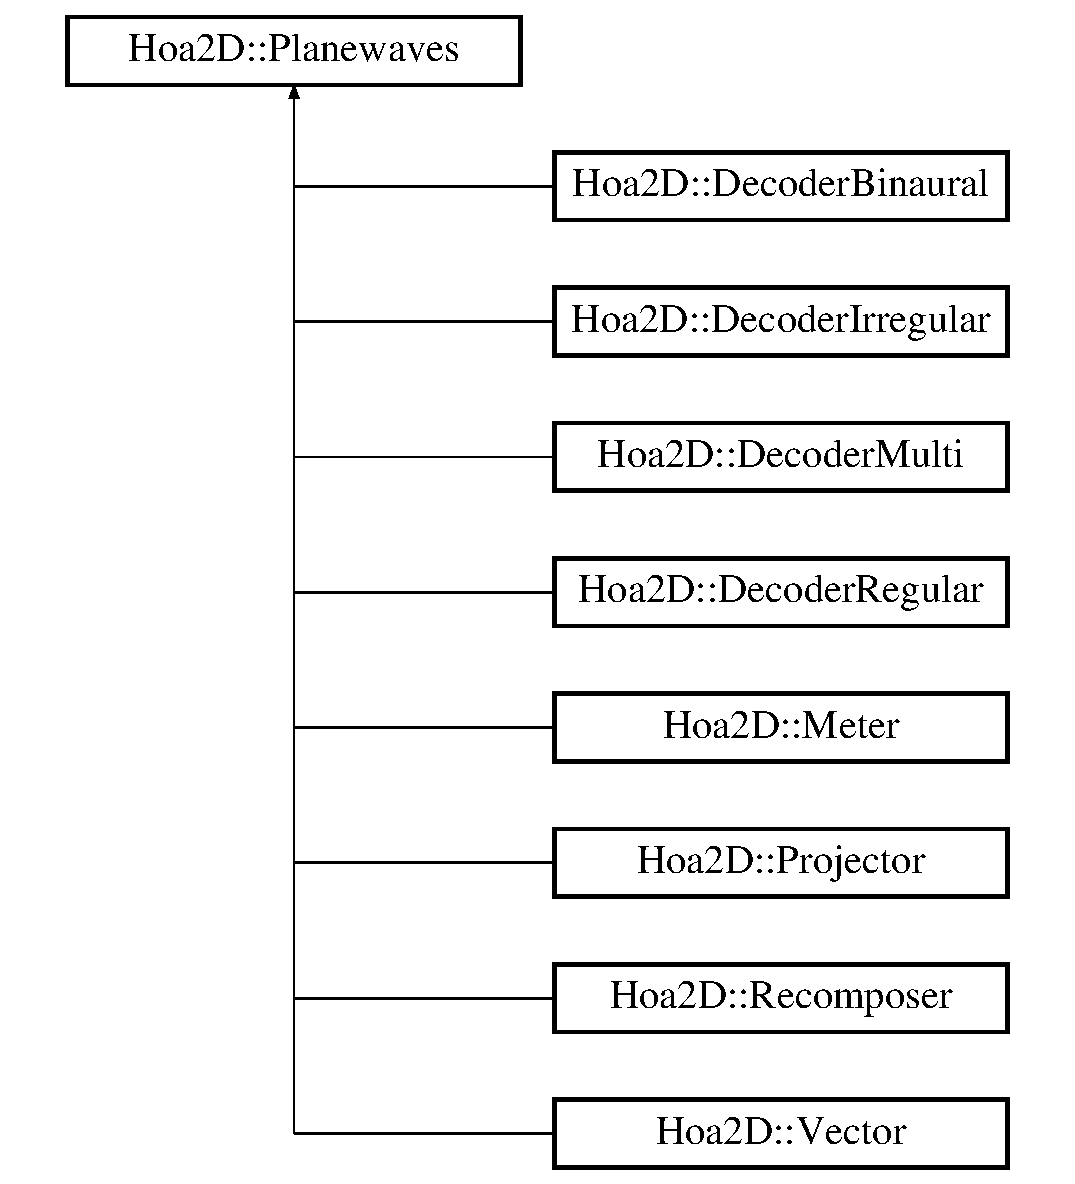
\includegraphics[height=9.000000cm]{class_hoa2_d_1_1_planewaves}
\end{center}
\end{figure}
\subsection*{Public Member Functions}
\begin{DoxyCompactItemize}
\item 
\hyperlink{class_hoa2_d_1_1_planewaves_ab233faf82900c5695b926214d6bbfff6}{Planewaves} (unsigned int number\-Of\-Channels)
\begin{DoxyCompactList}\small\item\em The planewaves constructor. \end{DoxyCompactList}\item 
\hyperlink{class_hoa2_d_1_1_planewaves_a7d13cc39051ae75f2af522651a1305bf}{$\sim$\-Planewaves} ()
\begin{DoxyCompactList}\small\item\em The planewaves destructor. \end{DoxyCompactList}\item 
unsigned int \hyperlink{class_hoa2_d_1_1_planewaves_a4bf0de6ae4ac7ac03fc552d477237a85}{get\-Number\-Of\-Channels} () const 
\begin{DoxyCompactList}\small\item\em Retrieve the number of channels. \end{DoxyCompactList}\item 
double \hyperlink{class_hoa2_d_1_1_planewaves_a52c4f8b05137ab56e82b0e076d7f5d3a}{get\-Channel\-Azimuth} (unsigned int index) const 
\begin{DoxyCompactList}\small\item\em Retrieve the azimuth of a channel. \end{DoxyCompactList}\item 
double \hyperlink{class_hoa2_d_1_1_planewaves_aab20597fa76482d7a907b2e39cc5be25}{get\-Channel\-Abscissa} (unsigned int index) const 
\begin{DoxyCompactList}\small\item\em Retrieve the abscissa of a channel. \end{DoxyCompactList}\item 
double \hyperlink{class_hoa2_d_1_1_planewaves_ade9d19725af0826e02b43bcf10a4bc73}{get\-Channel\-Ordinate} (unsigned int index) const 
\begin{DoxyCompactList}\small\item\em Retrieve the ordinate of a channel. \end{DoxyCompactList}\item 
std\-::string \hyperlink{class_hoa2_d_1_1_planewaves_a66b40a511ac3dd9f3ab1102e98370dbd}{get\-Channel\-Name} (unsigned int index)
\begin{DoxyCompactList}\small\item\em Retrieve a name for a channel. \end{DoxyCompactList}\end{DoxyCompactItemize}
\subsection*{Protected Member Functions}
\begin{DoxyCompactItemize}
\item 
void \hyperlink{class_hoa2_d_1_1_planewaves_a6f6dfb5355b12915c658ac8967303ef4}{set\-Channel\-Position} (unsigned int index, double azimuth)
\begin{DoxyCompactList}\small\item\em Set the azimuth of a channel. \end{DoxyCompactList}\end{DoxyCompactItemize}


\subsection{Detailed Description}
The planewaves class. 

The planewaves classes, that process on a set of channels (or planewaves), inherit from this class. It store basic informations like the number of channels, the coordinates and the names of channels. 

Definition at line 18 of file Planewaves.\-h.



\subsection{Constructor \& Destructor Documentation}
\hypertarget{class_hoa2_d_1_1_planewaves_ab233faf82900c5695b926214d6bbfff6}{\index{Hoa2\-D\-::\-Planewaves@{Hoa2\-D\-::\-Planewaves}!Planewaves@{Planewaves}}
\index{Planewaves@{Planewaves}!Hoa2D::Planewaves@{Hoa2\-D\-::\-Planewaves}}
\subsubsection[{Planewaves}]{\setlength{\rightskip}{0pt plus 5cm}Planewaves\-::\-Planewaves (
\begin{DoxyParamCaption}
\item[{unsigned int}]{number\-Of\-Channels}
\end{DoxyParamCaption}
)}}\label{class_hoa2_d_1_1_planewaves_ab233faf82900c5695b926214d6bbfff6}


The planewaves constructor. 

The lanewaves constructor allocates and initializes the general member values depending on a number of channels. The number of loudspkeakers must a least 1.


\begin{DoxyParams}{Parameters}
{\em number\-Of\-Channels} & The number of channels. \\
\hline
\end{DoxyParams}


Definition at line 11 of file Planewaves.\-cpp.

\hypertarget{class_hoa2_d_1_1_planewaves_a7d13cc39051ae75f2af522651a1305bf}{\index{Hoa2\-D\-::\-Planewaves@{Hoa2\-D\-::\-Planewaves}!$\sim$\-Planewaves@{$\sim$\-Planewaves}}
\index{$\sim$\-Planewaves@{$\sim$\-Planewaves}!Hoa2D::Planewaves@{Hoa2\-D\-::\-Planewaves}}
\subsubsection[{$\sim$\-Planewaves}]{\setlength{\rightskip}{0pt plus 5cm}Planewaves\-::$\sim$\-Planewaves (
\begin{DoxyParamCaption}
{}
\end{DoxyParamCaption}
)}}\label{class_hoa2_d_1_1_planewaves_a7d13cc39051ae75f2af522651a1305bf}


The planewaves destructor. 

The \hyperlink{class_hoa2_d_1_1_planewaves}{Planewaves} destructor free the memorie allocated. 

Definition at line 28 of file Planewaves.\-cpp.



\subsection{Member Function Documentation}
\hypertarget{class_hoa2_d_1_1_planewaves_aab20597fa76482d7a907b2e39cc5be25}{\index{Hoa2\-D\-::\-Planewaves@{Hoa2\-D\-::\-Planewaves}!get\-Channel\-Abscissa@{get\-Channel\-Abscissa}}
\index{get\-Channel\-Abscissa@{get\-Channel\-Abscissa}!Hoa2D::Planewaves@{Hoa2\-D\-::\-Planewaves}}
\subsubsection[{get\-Channel\-Abscissa}]{\setlength{\rightskip}{0pt plus 5cm}double Hoa2\-D\-::\-Planewaves\-::get\-Channel\-Abscissa (
\begin{DoxyParamCaption}
\item[{unsigned int}]{index}
\end{DoxyParamCaption}
) const\hspace{0.3cm}{\ttfamily [inline]}}}\label{class_hoa2_d_1_1_planewaves_aab20597fa76482d7a907b2e39cc5be25}


Retrieve the abscissa of a channel. 

Retrieve the abscissa of a channel. The abscissa is between -\/1 and 1, -\/1 is the left of the soundfield, 0 is the center of the soundfield and 1 is the right of the soundfield. The maximum index must be the number of channels -\/ 1.


\begin{DoxyParams}{Parameters}
{\em index} & The index of the loudspeaker. \\
\hline
\end{DoxyParams}
\begin{DoxyReturn}{Returns}
The abscissa of the channel if the channel exists, otherwise the function generates an error.
\end{DoxyReturn}
\begin{DoxySeeAlso}{See Also}
\hyperlink{class_hoa2_d_1_1_planewaves_a52c4f8b05137ab56e82b0e076d7f5d3a}{get\-Channel\-Azimuth} 

\hyperlink{class_hoa2_d_1_1_planewaves_ade9d19725af0826e02b43bcf10a4bc73}{get\-Channel\-Ordinate} 

\hyperlink{class_hoa2_d_1_1_planewaves_a66b40a511ac3dd9f3ab1102e98370dbd}{get\-Channel\-Name} 
\end{DoxySeeAlso}


Definition at line 84 of file Planewaves.\-h.

\hypertarget{class_hoa2_d_1_1_planewaves_a52c4f8b05137ab56e82b0e076d7f5d3a}{\index{Hoa2\-D\-::\-Planewaves@{Hoa2\-D\-::\-Planewaves}!get\-Channel\-Azimuth@{get\-Channel\-Azimuth}}
\index{get\-Channel\-Azimuth@{get\-Channel\-Azimuth}!Hoa2D::Planewaves@{Hoa2\-D\-::\-Planewaves}}
\subsubsection[{get\-Channel\-Azimuth}]{\setlength{\rightskip}{0pt plus 5cm}double Hoa2\-D\-::\-Planewaves\-::get\-Channel\-Azimuth (
\begin{DoxyParamCaption}
\item[{unsigned int}]{index}
\end{DoxyParamCaption}
) const\hspace{0.3cm}{\ttfamily [inline]}}}\label{class_hoa2_d_1_1_planewaves_a52c4f8b05137ab56e82b0e076d7f5d3a}


Retrieve the azimuth of a channel. 

Retrieve the azimuth of a channel. The azimuth of the channel is in radian, 0 radian is at the front of the soundfield and Pi is at the back of the sound field. The maximum index must be the number of channels -\/ 1.


\begin{DoxyParams}{Parameters}
{\em index} & The index of the channel. \\
\hline
\end{DoxyParams}
\begin{DoxyReturn}{Returns}
The azimuth of the channel if the channel exists, otherwise the function generates an error.
\end{DoxyReturn}
\begin{DoxySeeAlso}{See Also}
\hyperlink{class_hoa2_d_1_1_planewaves_aab20597fa76482d7a907b2e39cc5be25}{get\-Channel\-Abscissa} 

\hyperlink{class_hoa2_d_1_1_planewaves_ade9d19725af0826e02b43bcf10a4bc73}{get\-Channel\-Ordinate} 

\hyperlink{class_hoa2_d_1_1_planewaves_a66b40a511ac3dd9f3ab1102e98370dbd}{get\-Channel\-Name} 
\end{DoxySeeAlso}


Definition at line 67 of file Planewaves.\-h.

\hypertarget{class_hoa2_d_1_1_planewaves_a66b40a511ac3dd9f3ab1102e98370dbd}{\index{Hoa2\-D\-::\-Planewaves@{Hoa2\-D\-::\-Planewaves}!get\-Channel\-Name@{get\-Channel\-Name}}
\index{get\-Channel\-Name@{get\-Channel\-Name}!Hoa2D::Planewaves@{Hoa2\-D\-::\-Planewaves}}
\subsubsection[{get\-Channel\-Name}]{\setlength{\rightskip}{0pt plus 5cm}std\-::string Hoa2\-D\-::\-Planewaves\-::get\-Channel\-Name (
\begin{DoxyParamCaption}
\item[{unsigned int}]{index}
\end{DoxyParamCaption}
)\hspace{0.3cm}{\ttfamily [inline]}}}\label{class_hoa2_d_1_1_planewaves_a66b40a511ac3dd9f3ab1102e98370dbd}


Retrieve a name for a channel. 

Retrieve a name for a channel in a std\-::string format that will be \char`\"{}\-Channel index azimuth (in degrees)\char`\"{}.


\begin{DoxyParams}{Parameters}
{\em index} & The index of a channel. \\
\hline
\end{DoxyParams}
\begin{DoxyReturn}{Returns}
The method returns a name for the channel that contains its index and its azimuth if the channel exists, otherwise the function generates an error.
\end{DoxyReturn}
\begin{DoxySeeAlso}{See Also}
\hyperlink{class_hoa2_d_1_1_planewaves_a52c4f8b05137ab56e82b0e076d7f5d3a}{get\-Channel\-Azimuth} 

\hyperlink{class_hoa2_d_1_1_planewaves_aab20597fa76482d7a907b2e39cc5be25}{get\-Channel\-Abscissa} 

\hyperlink{class_hoa2_d_1_1_planewaves_ade9d19725af0826e02b43bcf10a4bc73}{get\-Channel\-Ordinate} 
\end{DoxySeeAlso}


Definition at line 116 of file Planewaves.\-h.

\hypertarget{class_hoa2_d_1_1_planewaves_ade9d19725af0826e02b43bcf10a4bc73}{\index{Hoa2\-D\-::\-Planewaves@{Hoa2\-D\-::\-Planewaves}!get\-Channel\-Ordinate@{get\-Channel\-Ordinate}}
\index{get\-Channel\-Ordinate@{get\-Channel\-Ordinate}!Hoa2D::Planewaves@{Hoa2\-D\-::\-Planewaves}}
\subsubsection[{get\-Channel\-Ordinate}]{\setlength{\rightskip}{0pt plus 5cm}double Hoa2\-D\-::\-Planewaves\-::get\-Channel\-Ordinate (
\begin{DoxyParamCaption}
\item[{unsigned int}]{index}
\end{DoxyParamCaption}
) const\hspace{0.3cm}{\ttfamily [inline]}}}\label{class_hoa2_d_1_1_planewaves_ade9d19725af0826e02b43bcf10a4bc73}


Retrieve the ordinate of a channel. 

Retrieve the ordinate of a channel. The ordinate is between -\/1 and 1, -\/1 is the back of the soundfield, 0 is the center of the soundfield and 1 is the front of the soundfield. The maximum index must be the number of channels -\/ 1.


\begin{DoxyParams}{Parameters}
{\em index} & The index of the channel. \\
\hline
\end{DoxyParams}
\begin{DoxyReturn}{Returns}
The ordinate of the channel if the channel exists, otherwise the function generates an error.
\end{DoxyReturn}
\begin{DoxySeeAlso}{See Also}
\hyperlink{class_hoa2_d_1_1_planewaves_a52c4f8b05137ab56e82b0e076d7f5d3a}{get\-Channel\-Azimuth} 

\hyperlink{class_hoa2_d_1_1_planewaves_aab20597fa76482d7a907b2e39cc5be25}{get\-Channel\-Abscissa} 

\hyperlink{class_hoa2_d_1_1_planewaves_a66b40a511ac3dd9f3ab1102e98370dbd}{get\-Channel\-Name} 
\end{DoxySeeAlso}


Definition at line 100 of file Planewaves.\-h.

\hypertarget{class_hoa2_d_1_1_planewaves_a4bf0de6ae4ac7ac03fc552d477237a85}{\index{Hoa2\-D\-::\-Planewaves@{Hoa2\-D\-::\-Planewaves}!get\-Number\-Of\-Channels@{get\-Number\-Of\-Channels}}
\index{get\-Number\-Of\-Channels@{get\-Number\-Of\-Channels}!Hoa2D::Planewaves@{Hoa2\-D\-::\-Planewaves}}
\subsubsection[{get\-Number\-Of\-Channels}]{\setlength{\rightskip}{0pt plus 5cm}unsigned int Hoa2\-D\-::\-Planewaves\-::get\-Number\-Of\-Channels (
\begin{DoxyParamCaption}
{}
\end{DoxyParamCaption}
) const\hspace{0.3cm}{\ttfamily [inline]}}}\label{class_hoa2_d_1_1_planewaves_a4bf0de6ae4ac7ac03fc552d477237a85}


Retrieve the number of channels. 

Retrieve the number of channels of the planewave class.

\begin{DoxyReturn}{Returns}
The number of channels. 
\end{DoxyReturn}


Definition at line 52 of file Planewaves.\-h.

\hypertarget{class_hoa2_d_1_1_planewaves_a6f6dfb5355b12915c658ac8967303ef4}{\index{Hoa2\-D\-::\-Planewaves@{Hoa2\-D\-::\-Planewaves}!set\-Channel\-Position@{set\-Channel\-Position}}
\index{set\-Channel\-Position@{set\-Channel\-Position}!Hoa2D::Planewaves@{Hoa2\-D\-::\-Planewaves}}
\subsubsection[{set\-Channel\-Position}]{\setlength{\rightskip}{0pt plus 5cm}void Planewaves\-::set\-Channel\-Position (
\begin{DoxyParamCaption}
\item[{unsigned int}]{index, }
\item[{double}]{azimuth}
\end{DoxyParamCaption}
)\hspace{0.3cm}{\ttfamily [protected]}}}\label{class_hoa2_d_1_1_planewaves_a6f6dfb5355b12915c658ac8967303ef4}


Set the azimuth of a channel. 

Set the azimuth of a channel. The azimuth is in radian between 0 and 2 Pi, O is the front of the soundfield and Pi is the back of the sound field. The maximum index must be the number of channel -\/ 1.


\begin{DoxyParams}{Parameters}
{\em index} & The index of the loudspeaker. \\
\hline
{\em azimuth} & The azimuth. \\
\hline
\end{DoxyParams}


Definition at line 22 of file Planewaves.\-cpp.



The documentation for this class was generated from the following files\-:\begin{DoxyCompactItemize}
\item 
/\-Users/\-Pierre/\-Source\-Tree/\-Hoa\-Library/\-Sources/\-Hoa2\-D/Planewaves.\-h\item 
/\-Users/\-Pierre/\-Source\-Tree/\-Hoa\-Library/\-Sources/\-Hoa2\-D/Planewaves.\-cpp\end{DoxyCompactItemize}

\hypertarget{class_hoa3_d_1_1_planewaves}{\section{Hoa3\-D\-:\-:Planewaves Class Reference}
\label{class_hoa3_d_1_1_planewaves}\index{Hoa3\-D\-::\-Planewaves@{Hoa3\-D\-::\-Planewaves}}
}


The planewaves class.  




{\ttfamily \#include $<$Planewaves.\-h$>$}

Inheritance diagram for Hoa3\-D\-:\-:Planewaves\-:\begin{figure}[H]
\begin{center}
\leavevmode
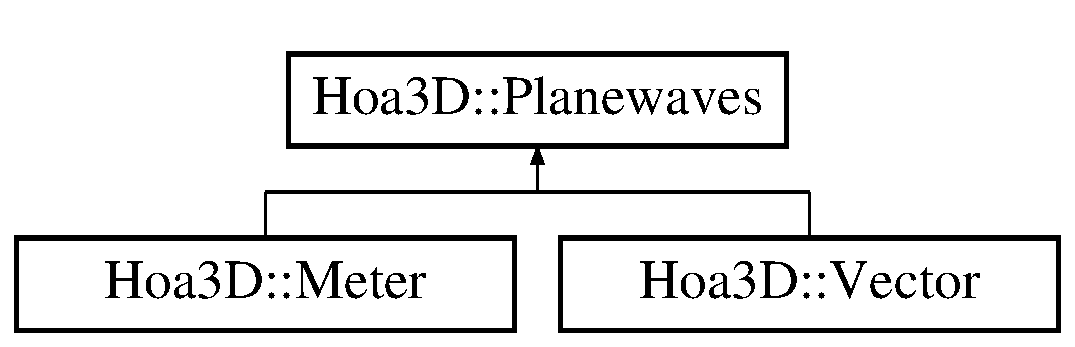
\includegraphics[height=2.000000cm]{class_hoa3_d_1_1_planewaves}
\end{center}
\end{figure}
\subsection*{Public Member Functions}
\begin{DoxyCompactItemize}
\item 
\hyperlink{class_hoa3_d_1_1_planewaves_ad190f41c56070493b4c55f4fcc9c6911}{Planewaves} (unsigned int number\-Of\-Loudspeakers)
\begin{DoxyCompactList}\small\item\em The planewaves constructor. \end{DoxyCompactList}\item 
\hyperlink{class_hoa3_d_1_1_planewaves_a51d3ba8bcdb8ad2e0c41e780f3c35d51}{$\sim$\-Planewaves} ()
\begin{DoxyCompactList}\small\item\em The planewaves destructor. \end{DoxyCompactList}\item 
void \hyperlink{class_hoa3_d_1_1_planewaves_ab39d630c1c191963cd35dd3b6a28ebc8}{set\-Loudspeaker\-Position} (unsigned int index, double azimuth, double elevation)
\begin{DoxyCompactList}\small\item\em Set the position of a loudspeaker. \end{DoxyCompactList}\item 
unsigned int \hyperlink{class_hoa3_d_1_1_planewaves_a467cdb1f079bb299225a9fac56a500e4}{get\-Number\-Of\-Loudspeakers} () const 
\begin{DoxyCompactList}\small\item\em Retrieve the number of loudspeakers. \end{DoxyCompactList}\item 
double \hyperlink{class_hoa3_d_1_1_planewaves_a8c0385dcf84e93ea035a91659122ce58}{get\-Loudspeaker\-Azimuth} (unsigned int index) const 
\begin{DoxyCompactList}\small\item\em Retrieve the azimuth of a loudspeaker. \end{DoxyCompactList}\item 
double \hyperlink{class_hoa3_d_1_1_planewaves_ae3b79c947e1923c5aad5067f7a2b29eb}{get\-Loudspeaker\-Elevation} (unsigned int index) const 
\begin{DoxyCompactList}\small\item\em Retrieve the elevation of a loudspeaker. \end{DoxyCompactList}\item 
double \hyperlink{class_hoa3_d_1_1_planewaves_ab88859d14af87a2766bcdb58f7d38b1c}{get\-Loudspeaker\-Abscissa} (unsigned int index) const 
\begin{DoxyCompactList}\small\item\em Retrieve the abscissa of a loudspeaker. \end{DoxyCompactList}\item 
double \hyperlink{class_hoa3_d_1_1_planewaves_a7bf08e3daaf9f9b1f66f5b8c7bde740f}{get\-Loudspeaker\-Ordinate} (unsigned int index) const 
\begin{DoxyCompactList}\small\item\em Retrieve the ordinate of a loudspeaker. \end{DoxyCompactList}\item 
double \hyperlink{class_hoa3_d_1_1_planewaves_acd3a7ad77d19ca916ecd8341bcf2c059}{get\-Loudspeaker\-Height} (unsigned int index) const 
\begin{DoxyCompactList}\small\item\em Retrieve the height of a loudspeaker. \end{DoxyCompactList}\item 
std\-::string \hyperlink{class_hoa3_d_1_1_planewaves_a264f20721feb71dd520a3ca115bfb141}{get\-Loudspeaker\-Name} (unsigned int index)
\begin{DoxyCompactList}\small\item\em Retrieve the number of loudspeaker. \end{DoxyCompactList}\end{DoxyCompactItemize}


\subsection{Detailed Description}
The planewaves class. 

The planewaves classes, that process on a set of loudspeakers, inherit from this class. It store basic informations like the number, the coordinates and the names of loudspeakers. 

Definition at line 19 of file Planewaves.\-h.



\subsection{Constructor \& Destructor Documentation}
\hypertarget{class_hoa3_d_1_1_planewaves_ad190f41c56070493b4c55f4fcc9c6911}{\index{Hoa3\-D\-::\-Planewaves@{Hoa3\-D\-::\-Planewaves}!Planewaves@{Planewaves}}
\index{Planewaves@{Planewaves}!Hoa3D::Planewaves@{Hoa3\-D\-::\-Planewaves}}
\subsubsection[{Planewaves}]{\setlength{\rightskip}{0pt plus 5cm}Hoa3\-D\-::\-Planewaves\-::\-Planewaves (
\begin{DoxyParamCaption}
\item[{unsigned int}]{number\-Of\-Loudspeakers}
\end{DoxyParamCaption}
)}}\label{class_hoa3_d_1_1_planewaves_ad190f41c56070493b4c55f4fcc9c6911}


The planewaves constructor. 

The lanewaves constructor allocates and initializes the general member values depending on a number of loudspeakers. The number of loudspkeakers must a least 1.


\begin{DoxyParams}{Parameters}
{\em number\-Of\-Loudspeakers} & The number of loudspeakers. \\
\hline
\end{DoxyParams}


Definition at line 11 of file Planewaves.\-cpp.

\hypertarget{class_hoa3_d_1_1_planewaves_a51d3ba8bcdb8ad2e0c41e780f3c35d51}{\index{Hoa3\-D\-::\-Planewaves@{Hoa3\-D\-::\-Planewaves}!$\sim$\-Planewaves@{$\sim$\-Planewaves}}
\index{$\sim$\-Planewaves@{$\sim$\-Planewaves}!Hoa3D::Planewaves@{Hoa3\-D\-::\-Planewaves}}
\subsubsection[{$\sim$\-Planewaves}]{\setlength{\rightskip}{0pt plus 5cm}Hoa3\-D\-::\-Planewaves\-::$\sim$\-Planewaves (
\begin{DoxyParamCaption}
{}
\end{DoxyParamCaption}
)}}\label{class_hoa3_d_1_1_planewaves_a51d3ba8bcdb8ad2e0c41e780f3c35d51}


The planewaves destructor. 

The \hyperlink{class_hoa3_d_1_1_planewaves}{Planewaves} destructor free the memorie allocated. 

Definition at line 26 of file Planewaves.\-cpp.



\subsection{Member Function Documentation}
\hypertarget{class_hoa3_d_1_1_planewaves_ab88859d14af87a2766bcdb58f7d38b1c}{\index{Hoa3\-D\-::\-Planewaves@{Hoa3\-D\-::\-Planewaves}!get\-Loudspeaker\-Abscissa@{get\-Loudspeaker\-Abscissa}}
\index{get\-Loudspeaker\-Abscissa@{get\-Loudspeaker\-Abscissa}!Hoa3D::Planewaves@{Hoa3\-D\-::\-Planewaves}}
\subsubsection[{get\-Loudspeaker\-Abscissa}]{\setlength{\rightskip}{0pt plus 5cm}double Hoa3\-D\-::\-Planewaves\-::get\-Loudspeaker\-Abscissa (
\begin{DoxyParamCaption}
\item[{unsigned int}]{index}
\end{DoxyParamCaption}
) const\hspace{0.3cm}{\ttfamily [inline]}}}\label{class_hoa3_d_1_1_planewaves_ab88859d14af87a2766bcdb58f7d38b1c}


Retrieve the abscissa of a loudspeaker. 

Retrieve the abscissa of a loudspeaker. The abscissa is between -\/1 and 1, -\/1 is the left of the soundfield, 0 is the center of the soundfield and 1 is the right of the soundfield. The maximum index must be the number of loudspeakers -\/ 1.


\begin{DoxyParams}{Parameters}
{\em index} & The index of the loudspeaker. \\
\hline
\end{DoxyParams}
\begin{DoxyReturn}{Returns}
The abscissa of the loudspeaker. 
\end{DoxyReturn}
\begin{DoxySeeAlso}{See Also}
\hyperlink{class_hoa3_d_1_1_planewaves_a7bf08e3daaf9f9b1f66f5b8c7bde740f}{get\-Loudspeaker\-Ordinate} 

\hyperlink{class_hoa3_d_1_1_planewaves_acd3a7ad77d19ca916ecd8341bcf2c059}{get\-Loudspeaker\-Height} 
\end{DoxySeeAlso}


Definition at line 91 of file Planewaves.\-h.

\hypertarget{class_hoa3_d_1_1_planewaves_a8c0385dcf84e93ea035a91659122ce58}{\index{Hoa3\-D\-::\-Planewaves@{Hoa3\-D\-::\-Planewaves}!get\-Loudspeaker\-Azimuth@{get\-Loudspeaker\-Azimuth}}
\index{get\-Loudspeaker\-Azimuth@{get\-Loudspeaker\-Azimuth}!Hoa3D::Planewaves@{Hoa3\-D\-::\-Planewaves}}
\subsubsection[{get\-Loudspeaker\-Azimuth}]{\setlength{\rightskip}{0pt plus 5cm}double Hoa3\-D\-::\-Planewaves\-::get\-Loudspeaker\-Azimuth (
\begin{DoxyParamCaption}
\item[{unsigned int}]{index}
\end{DoxyParamCaption}
) const\hspace{0.3cm}{\ttfamily [inline]}}}\label{class_hoa3_d_1_1_planewaves_a8c0385dcf84e93ea035a91659122ce58}


Retrieve the azimuth of a loudspeaker. 

Retrieve the azimuth of a loudspeaker. The azimuth of the loudspeaker is in radian, 0 radian is at the front of the soundfield and Pi is at the back of the sound field. The maximum index must be the number of loudspeakers -\/ 1.


\begin{DoxyParams}{Parameters}
{\em index} & The index of the loudspeaker. \\
\hline
\end{DoxyParams}
\begin{DoxyReturn}{Returns}
The azimuth of the loudspeaker. 
\end{DoxyReturn}
\begin{DoxySeeAlso}{See Also}
\hyperlink{class_hoa3_d_1_1_planewaves_ae3b79c947e1923c5aad5067f7a2b29eb}{get\-Loudspeaker\-Elevation} 
\end{DoxySeeAlso}


Definition at line 64 of file Planewaves.\-h.

\hypertarget{class_hoa3_d_1_1_planewaves_ae3b79c947e1923c5aad5067f7a2b29eb}{\index{Hoa3\-D\-::\-Planewaves@{Hoa3\-D\-::\-Planewaves}!get\-Loudspeaker\-Elevation@{get\-Loudspeaker\-Elevation}}
\index{get\-Loudspeaker\-Elevation@{get\-Loudspeaker\-Elevation}!Hoa3D::Planewaves@{Hoa3\-D\-::\-Planewaves}}
\subsubsection[{get\-Loudspeaker\-Elevation}]{\setlength{\rightskip}{0pt plus 5cm}double Hoa3\-D\-::\-Planewaves\-::get\-Loudspeaker\-Elevation (
\begin{DoxyParamCaption}
\item[{unsigned int}]{index}
\end{DoxyParamCaption}
) const\hspace{0.3cm}{\ttfamily [inline]}}}\label{class_hoa3_d_1_1_planewaves_ae3b79c947e1923c5aad5067f7a2b29eb}


Retrieve the elevation of a loudspeaker. 

Retrieve the elevation of a loudspeaker. The elevation is in radian between -\/1/2 Pi and 1/2 Pi, -\/1/2 Pi the the bottom of the sound field, 0 is the center of the sound field and 1/2 Pi is the top of the sound field. The maximum index must be the number of loudspeakers -\/ 1.


\begin{DoxyParams}{Parameters}
{\em index} & The index of the loudspeaker. \\
\hline
\end{DoxyParams}
\begin{DoxyReturn}{Returns}
The elevation of the loudspeaker. 
\end{DoxyReturn}
\begin{DoxySeeAlso}{See Also}
\hyperlink{class_hoa3_d_1_1_planewaves_a8c0385dcf84e93ea035a91659122ce58}{get\-Loudspeaker\-Azimuth} 
\end{DoxySeeAlso}


Definition at line 77 of file Planewaves.\-h.

\hypertarget{class_hoa3_d_1_1_planewaves_acd3a7ad77d19ca916ecd8341bcf2c059}{\index{Hoa3\-D\-::\-Planewaves@{Hoa3\-D\-::\-Planewaves}!get\-Loudspeaker\-Height@{get\-Loudspeaker\-Height}}
\index{get\-Loudspeaker\-Height@{get\-Loudspeaker\-Height}!Hoa3D::Planewaves@{Hoa3\-D\-::\-Planewaves}}
\subsubsection[{get\-Loudspeaker\-Height}]{\setlength{\rightskip}{0pt plus 5cm}double Hoa3\-D\-::\-Planewaves\-::get\-Loudspeaker\-Height (
\begin{DoxyParamCaption}
\item[{unsigned int}]{index}
\end{DoxyParamCaption}
) const\hspace{0.3cm}{\ttfamily [inline]}}}\label{class_hoa3_d_1_1_planewaves_acd3a7ad77d19ca916ecd8341bcf2c059}


Retrieve the height of a loudspeaker. 

Retrieve the height of a loudspeaker. The height is between -\/1 and 1, -\/1 is the bottom of the soundfield, 0 is the center of the soundfield and 1 is the top of the soundfield. The maximum index must be the number of loudspeakers -\/ 1.


\begin{DoxyParams}{Parameters}
{\em index} & The index of the loudspeaker. \\
\hline
\end{DoxyParams}
\begin{DoxyReturn}{Returns}
The height of the loudspeaker. 
\end{DoxyReturn}
\begin{DoxySeeAlso}{See Also}
\hyperlink{class_hoa3_d_1_1_planewaves_ab88859d14af87a2766bcdb58f7d38b1c}{get\-Loudspeaker\-Abscissa} 

\hyperlink{class_hoa3_d_1_1_planewaves_a7bf08e3daaf9f9b1f66f5b8c7bde740f}{get\-Loudspeaker\-Ordinate} 
\end{DoxySeeAlso}


Definition at line 119 of file Planewaves.\-h.

\hypertarget{class_hoa3_d_1_1_planewaves_a264f20721feb71dd520a3ca115bfb141}{\index{Hoa3\-D\-::\-Planewaves@{Hoa3\-D\-::\-Planewaves}!get\-Loudspeaker\-Name@{get\-Loudspeaker\-Name}}
\index{get\-Loudspeaker\-Name@{get\-Loudspeaker\-Name}!Hoa3D::Planewaves@{Hoa3\-D\-::\-Planewaves}}
\subsubsection[{get\-Loudspeaker\-Name}]{\setlength{\rightskip}{0pt plus 5cm}std\-::string Hoa3\-D\-::\-Planewaves\-::get\-Loudspeaker\-Name (
\begin{DoxyParamCaption}
\item[{unsigned int}]{index}
\end{DoxyParamCaption}
)\hspace{0.3cm}{\ttfamily [inline]}}}\label{class_hoa3_d_1_1_planewaves_a264f20721feb71dd520a3ca115bfb141}


Retrieve the number of loudspeaker. 

Retrieve a name for an loudspeaker in a std\-::string format that will be \char`\"{}\-Loudspeaker index azimuth elevation\char`\"{}.


\begin{DoxyParams}{Parameters}
{\em index} & The global index of a loudspeaker. \\
\hline
\end{DoxyParams}
\begin{DoxyReturn}{Returns}
The name of the loudspeaker 
\end{DoxyReturn}


Definition at line 131 of file Planewaves.\-h.

\hypertarget{class_hoa3_d_1_1_planewaves_a7bf08e3daaf9f9b1f66f5b8c7bde740f}{\index{Hoa3\-D\-::\-Planewaves@{Hoa3\-D\-::\-Planewaves}!get\-Loudspeaker\-Ordinate@{get\-Loudspeaker\-Ordinate}}
\index{get\-Loudspeaker\-Ordinate@{get\-Loudspeaker\-Ordinate}!Hoa3D::Planewaves@{Hoa3\-D\-::\-Planewaves}}
\subsubsection[{get\-Loudspeaker\-Ordinate}]{\setlength{\rightskip}{0pt plus 5cm}double Hoa3\-D\-::\-Planewaves\-::get\-Loudspeaker\-Ordinate (
\begin{DoxyParamCaption}
\item[{unsigned int}]{index}
\end{DoxyParamCaption}
) const\hspace{0.3cm}{\ttfamily [inline]}}}\label{class_hoa3_d_1_1_planewaves_a7bf08e3daaf9f9b1f66f5b8c7bde740f}


Retrieve the ordinate of a loudspeaker. 

Retrieve the ordinate of a loudspeaker. The ordinate is between -\/1 and 1, -\/1 is the back of the soundfield, 0 is the center of the soundfield and 1 is the front of the soundfield. The maximum index must be the number of loudspeakers -\/ 1.


\begin{DoxyParams}{Parameters}
{\em index} & The index of the loudspeaker. \\
\hline
\end{DoxyParams}
\begin{DoxyReturn}{Returns}
The ordinate of the loudspeaker. 
\end{DoxyReturn}
\begin{DoxySeeAlso}{See Also}
\hyperlink{class_hoa3_d_1_1_planewaves_ab88859d14af87a2766bcdb58f7d38b1c}{get\-Loudspeaker\-Abscissa} 

\hyperlink{class_hoa3_d_1_1_planewaves_acd3a7ad77d19ca916ecd8341bcf2c059}{get\-Loudspeaker\-Height} 
\end{DoxySeeAlso}


Definition at line 105 of file Planewaves.\-h.

\hypertarget{class_hoa3_d_1_1_planewaves_a467cdb1f079bb299225a9fac56a500e4}{\index{Hoa3\-D\-::\-Planewaves@{Hoa3\-D\-::\-Planewaves}!get\-Number\-Of\-Loudspeakers@{get\-Number\-Of\-Loudspeakers}}
\index{get\-Number\-Of\-Loudspeakers@{get\-Number\-Of\-Loudspeakers}!Hoa3D::Planewaves@{Hoa3\-D\-::\-Planewaves}}
\subsubsection[{get\-Number\-Of\-Loudspeakers}]{\setlength{\rightskip}{0pt plus 5cm}unsigned int Hoa3\-D\-::\-Planewaves\-::get\-Number\-Of\-Loudspeakers (
\begin{DoxyParamCaption}
{}
\end{DoxyParamCaption}
) const\hspace{0.3cm}{\ttfamily [inline]}}}\label{class_hoa3_d_1_1_planewaves_a467cdb1f079bb299225a9fac56a500e4}


Retrieve the number of loudspeakers. 

Retrieve the number of loudspeakers of the planewave class.

\begin{DoxyReturn}{Returns}
The number of loudspeakers. 
\end{DoxyReturn}


Definition at line 55 of file Planewaves.\-h.

\hypertarget{class_hoa3_d_1_1_planewaves_ab39d630c1c191963cd35dd3b6a28ebc8}{\index{Hoa3\-D\-::\-Planewaves@{Hoa3\-D\-::\-Planewaves}!set\-Loudspeaker\-Position@{set\-Loudspeaker\-Position}}
\index{set\-Loudspeaker\-Position@{set\-Loudspeaker\-Position}!Hoa3D::Planewaves@{Hoa3\-D\-::\-Planewaves}}
\subsubsection[{set\-Loudspeaker\-Position}]{\setlength{\rightskip}{0pt plus 5cm}void Hoa3\-D\-::\-Planewaves\-::set\-Loudspeaker\-Position (
\begin{DoxyParamCaption}
\item[{unsigned int}]{index, }
\item[{double}]{azimuth, }
\item[{double}]{elevation}
\end{DoxyParamCaption}
)}}\label{class_hoa3_d_1_1_planewaves_ab39d630c1c191963cd35dd3b6a28ebc8}


Set the position of a loudspeaker. 

Set the position of a loudspeaker with polar coordinates. The azimtuh is in radian between 0 and 2 Pi, O is the front of the soundfield and Pi is the back of the sound field. The elevation is in radian between -\/1/2 Pi and 1/2 Pi, -\/1/2 Pi the the bottom of the sound field, 0 is the center of the sound field and 1/2 Pi is the top of the sound field. The maximum index must be the number of loudspeakers -\/ 1.


\begin{DoxyParams}{Parameters}
{\em index} & The index of the loudspeaker. \\
\hline
{\em azimuth} & The azimuth. \\
\hline
{\em elevation} & The elevation. \\
\hline
\end{DoxyParams}


Definition at line 19 of file Planewaves.\-cpp.


\hypertarget{class_hoa2_d_1_1_projector}{\section{Hoa2\-D\-:\-:Projector Class Reference}
\label{class_hoa2_d_1_1_projector}\index{Hoa2\-D\-::\-Projector@{Hoa2\-D\-::\-Projector}}
}


The ambisonic projector.  




{\ttfamily \#include $<$Projector.\-h$>$}

Inheritance diagram for Hoa2\-D\-:\-:Projector\-:\begin{figure}[H]
\begin{center}
\leavevmode
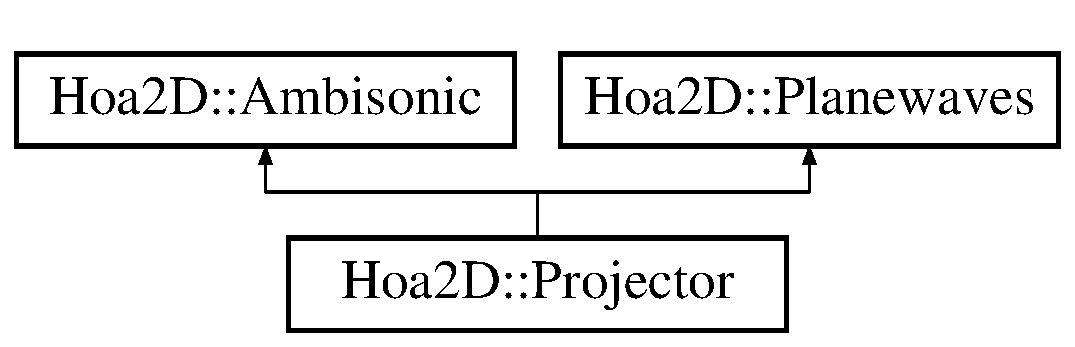
\includegraphics[height=2.000000cm]{class_hoa2_d_1_1_projector}
\end{center}
\end{figure}
\subsection*{Public Member Functions}
\begin{DoxyCompactItemize}
\item 
\hyperlink{class_hoa2_d_1_1_projector_a73b651a38b0680e6da45242073af54b7}{Projector} (unsigned int order, unsigned int number\-Of\-Channels)
\begin{DoxyCompactList}\small\item\em The projector constructor. \end{DoxyCompactList}\item 
\hyperlink{class_hoa2_d_1_1_projector_a7a93c4c33578b5f09636790a048c1351}{$\sim$\-Projector} ()
\begin{DoxyCompactList}\small\item\em The projector destructor. \end{DoxyCompactList}\item 
void \hyperlink{class_hoa2_d_1_1_projector_a3c4e52a53212701d92d5d5bff7af225b}{process} (const float $\ast$inputs, float $\ast$outputs)
\begin{DoxyCompactList}\small\item\em This method performs the projection with single precision. \end{DoxyCompactList}\item 
void \hyperlink{class_hoa2_d_1_1_projector_a60fe345d15f928b55a3755edb6f5026c}{process} (const double $\ast$inputs, double $\ast$outputs)
\begin{DoxyCompactList}\small\item\em This method performs the projection with double precision. \end{DoxyCompactList}\end{DoxyCompactItemize}


\subsection{Detailed Description}
The ambisonic projector. 

The projector should be used to projects the circular harmonics on a circle and to give access to the planewaves domain. The projection is similar to the decoding exept that the circle discretization cannot be defined be the user. Then the number of channels (or planewaves) must be a least the number of harmonics, the first angle is 0 radian and the angular distances between the channels are equals. 

Definition at line 19 of file Projector.\-h.



\subsection{Constructor \& Destructor Documentation}
\hypertarget{class_hoa2_d_1_1_projector_a73b651a38b0680e6da45242073af54b7}{\index{Hoa2\-D\-::\-Projector@{Hoa2\-D\-::\-Projector}!Projector@{Projector}}
\index{Projector@{Projector}!Hoa2D::Projector@{Hoa2\-D\-::\-Projector}}
\subsubsection[{Projector}]{\setlength{\rightskip}{0pt plus 5cm}Hoa2\-D\-::\-Projector\-::\-Projector (
\begin{DoxyParamCaption}
\item[{unsigned int}]{order, }
\item[{unsigned int}]{number\-Of\-Channels}
\end{DoxyParamCaption}
)}}\label{class_hoa2_d_1_1_projector_a73b651a38b0680e6da45242073af54b7}


The projector constructor. 

The projector constructor allocates and initialize the member values to project the circular harmonics on a circle. The order must be at least 1 and the number of channels must be a least the number of harmonics.


\begin{DoxyParams}{Parameters}
{\em order} & The order. \\
\hline
{\em number\-Of\-Channels} & The number of channels. \\
\hline
\end{DoxyParams}


Definition at line 11 of file Projector.\-cpp.

\hypertarget{class_hoa2_d_1_1_projector_a7a93c4c33578b5f09636790a048c1351}{\index{Hoa2\-D\-::\-Projector@{Hoa2\-D\-::\-Projector}!$\sim$\-Projector@{$\sim$\-Projector}}
\index{$\sim$\-Projector@{$\sim$\-Projector}!Hoa2D::Projector@{Hoa2\-D\-::\-Projector}}
\subsubsection[{$\sim$\-Projector}]{\setlength{\rightskip}{0pt plus 5cm}Hoa2\-D\-::\-Projector\-::$\sim$\-Projector (
\begin{DoxyParamCaption}
{}
\end{DoxyParamCaption}
)}}\label{class_hoa2_d_1_1_projector_a7a93c4c33578b5f09636790a048c1351}


The projector destructor. 

The projector destructor free the memory. 

Definition at line 41 of file Projector.\-cpp.



\subsection{Member Function Documentation}
\hypertarget{class_hoa2_d_1_1_projector_a3c4e52a53212701d92d5d5bff7af225b}{\index{Hoa2\-D\-::\-Projector@{Hoa2\-D\-::\-Projector}!process@{process}}
\index{process@{process}!Hoa2D::Projector@{Hoa2\-D\-::\-Projector}}
\subsubsection[{process}]{\setlength{\rightskip}{0pt plus 5cm}void Hoa2\-D\-::\-Projector\-::process (
\begin{DoxyParamCaption}
\item[{const float $\ast$}]{inputs, }
\item[{float $\ast$}]{outputs}
\end{DoxyParamCaption}
)}}\label{class_hoa2_d_1_1_projector_a3c4e52a53212701d92d5d5bff7af225b}


This method performs the projection with single precision. 

You should use this method for in-\/place or not-\/in-\/place processing and performs the projection sample by sample. The inputs array contains the circular harmonics samples and the minimum size must be the number of harmonics and the outputs array contains the channels (or planewaves) samples and the minimum size must be a least the number of channels.


\begin{DoxyParams}{Parameters}
{\em inputs} & The inputs array. \\
\hline
{\em outputs} & The outputs array. \\
\hline
\end{DoxyParams}


Definition at line 31 of file Projector.\-cpp.

\hypertarget{class_hoa2_d_1_1_projector_a60fe345d15f928b55a3755edb6f5026c}{\index{Hoa2\-D\-::\-Projector@{Hoa2\-D\-::\-Projector}!process@{process}}
\index{process@{process}!Hoa2D::Projector@{Hoa2\-D\-::\-Projector}}
\subsubsection[{process}]{\setlength{\rightskip}{0pt plus 5cm}void Hoa2\-D\-::\-Projector\-::process (
\begin{DoxyParamCaption}
\item[{const double $\ast$}]{inputs, }
\item[{double $\ast$}]{outputs}
\end{DoxyParamCaption}
)}}\label{class_hoa2_d_1_1_projector_a60fe345d15f928b55a3755edb6f5026c}


This method performs the projection with double precision. 

You should use this method for in-\/place or not-\/in-\/place processing and performs the projection sample by sample. The inputs array contains the circular harmonics samples and the minimum size must be the number of harmonics and the outputs array contains the channels (or planewaves) samples and the minimum size must be a least the number of channels.


\begin{DoxyParams}{Parameters}
{\em inputs} & The inputs array. \\
\hline
{\em outputs} & The outputs array. \\
\hline
\end{DoxyParams}


Definition at line 36 of file Projector.\-cpp.



The documentation for this class was generated from the following files\-:\begin{DoxyCompactItemize}
\item 
/\-Users/\-Pierre/\-Source\-Tree/\-Hoa\-Library/\-Sources/\-Hoa2\-D/Projector.\-h\item 
/\-Users/\-Pierre/\-Source\-Tree/\-Hoa\-Library/\-Sources/\-Hoa2\-D/Projector.\-cpp\end{DoxyCompactItemize}

\hypertarget{class_hoa2_d_1_1_recomposer}{\section{Hoa2\-D\-:\-:Recomposer Class Reference}
\label{class_hoa2_d_1_1_recomposer}\index{Hoa2\-D\-::\-Recomposer@{Hoa2\-D\-::\-Recomposer}}
}


The ambisonic recomposer.  




{\ttfamily \#include $<$Recomposer.\-h$>$}

Inheritance diagram for Hoa2\-D\-:\-:Recomposer\-:\begin{figure}[H]
\begin{center}
\leavevmode
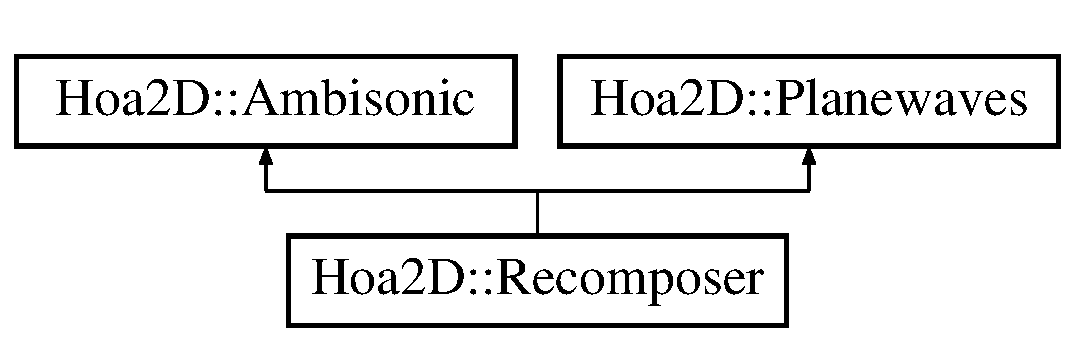
\includegraphics[height=2.000000cm]{class_hoa2_d_1_1_recomposer}
\end{center}
\end{figure}
\subsection*{Public Member Functions}
\begin{DoxyCompactItemize}
\item 
\hyperlink{class_hoa2_d_1_1_recomposer_aa5feded7afd2329099583b245d276140}{Recomposer} (unsigned int order, unsigned int number\-Of\-Channels)
\begin{DoxyCompactList}\small\item\em The recomposer constructor. \end{DoxyCompactList}\item 
\hyperlink{class_hoa2_d_1_1_recomposer_a6e26043adf8b785d746084dfed82f183}{$\sim$\-Recomposer} ()
\begin{DoxyCompactList}\small\item\em The recomposer destructor. \end{DoxyCompactList}\item 
void \hyperlink{class_hoa2_d_1_1_recomposer_a2c1827fa0b25648b787077469e52a820}{set\-Azimuth} (unsigned int index, const double azimuth)
\begin{DoxyCompactList}\small\item\em This method set the angle of azimuth of a channel. \end{DoxyCompactList}\item 
void \hyperlink{class_hoa2_d_1_1_recomposer_aea7c383166c6c40c5605175b18a19ad1}{set\-Widening\-Value} (unsigned int index, const double value)
\begin{DoxyCompactList}\small\item\em This method set the widening value of a channel. \end{DoxyCompactList}\item 
double \hyperlink{class_hoa2_d_1_1_recomposer_a81bc1f97e61543558a0595f4fd8a4e46}{get\-Azimuth} (unsigned int index) const 
\begin{DoxyCompactList}\small\item\em This method retrieve the azimuth of a channel. \end{DoxyCompactList}\item 
double \hyperlink{class_hoa2_d_1_1_recomposer_a31d6045c32e191a7c5212e4e34d6d3ab}{get\-Widening\-Value} (unsigned int index) const 
\begin{DoxyCompactList}\small\item\em This method retrieve the widening value of a channel. \end{DoxyCompactList}\item 
void \hyperlink{class_hoa2_d_1_1_recomposer_a92050d70682a94814e8b772daf8b4717}{process} (const float $\ast$inputs, float $\ast$outputs)
\begin{DoxyCompactList}\small\item\em This method performs the recomposition with single precision. \end{DoxyCompactList}\item 
void \hyperlink{class_hoa2_d_1_1_recomposer_a34bb1c0970dc3fa40a3bf90b47e5d5d1}{process} (const double $\ast$inputs, double $\ast$outputs)
\begin{DoxyCompactList}\small\item\em This method performs the recomposition with double precision. \end{DoxyCompactList}\end{DoxyCompactItemize}
\subsection*{Additional Inherited Members}


\subsection{Detailed Description}
The ambisonic recomposer. 

The recomposer should be in the planewaves domain to come back the the circular harmonics domain. The recomposition is similar to the several encoding exept that we consider planewaves (or virtual microphones) instead of sources. The number of channels (or planewaves) must be a least the number of harmonics, the first angle is 0 radian and the angular distances between the channels are equals. 

Definition at line 20 of file Recomposer.\-h.



\subsection{Constructor \& Destructor Documentation}
\hypertarget{class_hoa2_d_1_1_recomposer_aa5feded7afd2329099583b245d276140}{\index{Hoa2\-D\-::\-Recomposer@{Hoa2\-D\-::\-Recomposer}!Recomposer@{Recomposer}}
\index{Recomposer@{Recomposer}!Hoa2D::Recomposer@{Hoa2\-D\-::\-Recomposer}}
\subsubsection[{Recomposer}]{\setlength{\rightskip}{0pt plus 5cm}Hoa2\-D\-::\-Recomposer\-::\-Recomposer (
\begin{DoxyParamCaption}
\item[{unsigned int}]{order, }
\item[{unsigned int}]{number\-Of\-Channels}
\end{DoxyParamCaption}
)}}\label{class_hoa2_d_1_1_recomposer_aa5feded7afd2329099583b245d276140}


The recomposer constructor. 

The recomposer constructor allocates and initialize the member values to recompose a set of planewaves in the circular harmonics domain. The order must be at least 1 and the number of channels must be a least the number of harmonics.


\begin{DoxyParams}{Parameters}
{\em order} & The order. \\
\hline
{\em number\-Of\-Channels} & The number of channels. \\
\hline
\end{DoxyParams}


Definition at line 11 of file Recomposer.\-cpp.

\hypertarget{class_hoa2_d_1_1_recomposer_a6e26043adf8b785d746084dfed82f183}{\index{Hoa2\-D\-::\-Recomposer@{Hoa2\-D\-::\-Recomposer}!$\sim$\-Recomposer@{$\sim$\-Recomposer}}
\index{$\sim$\-Recomposer@{$\sim$\-Recomposer}!Hoa2D::Recomposer@{Hoa2\-D\-::\-Recomposer}}
\subsubsection[{$\sim$\-Recomposer}]{\setlength{\rightskip}{0pt plus 5cm}Hoa2\-D\-::\-Recomposer\-::$\sim$\-Recomposer (
\begin{DoxyParamCaption}
{}
\end{DoxyParamCaption}
)}}\label{class_hoa2_d_1_1_recomposer_a6e26043adf8b785d746084dfed82f183}


The recomposer destructor. 

The recomposer destructor free the memory. 

Definition at line 60 of file Recomposer.\-cpp.



\subsection{Member Function Documentation}
\hypertarget{class_hoa2_d_1_1_recomposer_a81bc1f97e61543558a0595f4fd8a4e46}{\index{Hoa2\-D\-::\-Recomposer@{Hoa2\-D\-::\-Recomposer}!get\-Azimuth@{get\-Azimuth}}
\index{get\-Azimuth@{get\-Azimuth}!Hoa2D::Recomposer@{Hoa2\-D\-::\-Recomposer}}
\subsubsection[{get\-Azimuth}]{\setlength{\rightskip}{0pt plus 5cm}double Hoa2\-D\-::\-Recomposer\-::get\-Azimuth (
\begin{DoxyParamCaption}
\item[{unsigned int}]{index}
\end{DoxyParamCaption}
) const\hspace{0.3cm}{\ttfamily [inline]}}}\label{class_hoa2_d_1_1_recomposer_a81bc1f97e61543558a0595f4fd8a4e46}


This method retrieve the azimuth of a channel. 

Retrieve the azimuth of a source.


\begin{DoxyParams}{Parameters}
{\em index} & The index of the channel. \\
\hline
\end{DoxyParams}
\begin{DoxyReturn}{Returns}
The azimuth of the channel if the channel exists, otherwise the function generates an error. 
\end{DoxyReturn}


Definition at line 68 of file Recomposer.\-h.

\hypertarget{class_hoa2_d_1_1_recomposer_a31d6045c32e191a7c5212e4e34d6d3ab}{\index{Hoa2\-D\-::\-Recomposer@{Hoa2\-D\-::\-Recomposer}!get\-Widening\-Value@{get\-Widening\-Value}}
\index{get\-Widening\-Value@{get\-Widening\-Value}!Hoa2D::Recomposer@{Hoa2\-D\-::\-Recomposer}}
\subsubsection[{get\-Widening\-Value}]{\setlength{\rightskip}{0pt plus 5cm}double Hoa2\-D\-::\-Recomposer\-::get\-Widening\-Value (
\begin{DoxyParamCaption}
\item[{unsigned int}]{index}
\end{DoxyParamCaption}
) const\hspace{0.3cm}{\ttfamily [inline]}}}\label{class_hoa2_d_1_1_recomposer_a31d6045c32e191a7c5212e4e34d6d3ab}


This method retrieve the widening value of a channel. 

Retrieve the widening value of a channel.


\begin{DoxyParams}{Parameters}
{\em index} & The index of the channel. \\
\hline
\end{DoxyParams}
\begin{DoxyReturn}{Returns}
The widening value of the channel if the channel exists, otherwise the function generates an error. 
\end{DoxyReturn}


Definition at line 80 of file Recomposer.\-h.

\hypertarget{class_hoa2_d_1_1_recomposer_a92050d70682a94814e8b772daf8b4717}{\index{Hoa2\-D\-::\-Recomposer@{Hoa2\-D\-::\-Recomposer}!process@{process}}
\index{process@{process}!Hoa2D::Recomposer@{Hoa2\-D\-::\-Recomposer}}
\subsubsection[{process}]{\setlength{\rightskip}{0pt plus 5cm}void Hoa2\-D\-::\-Recomposer\-::process (
\begin{DoxyParamCaption}
\item[{const float $\ast$}]{inputs, }
\item[{float $\ast$}]{outputs}
\end{DoxyParamCaption}
)}}\label{class_hoa2_d_1_1_recomposer_a92050d70682a94814e8b772daf8b4717}


This method performs the recomposition with single precision. 

You should use this method for in-\/place or not-\/in-\/place processing and performs the projection sample by sample. The outputs array contains the circular harmonics samples and the minimum size must be the number of harmonics and the inputs array contains the channels (or planewaves) samples and the minimum size must be a least the number of channels.


\begin{DoxyParams}{Parameters}
{\em inputs} & The inputs array. \\
\hline
{\em outputs} & The outputs array. \\
\hline
\end{DoxyParams}


Definition at line 36 of file Recomposer.\-cpp.

\hypertarget{class_hoa2_d_1_1_recomposer_a34bb1c0970dc3fa40a3bf90b47e5d5d1}{\index{Hoa2\-D\-::\-Recomposer@{Hoa2\-D\-::\-Recomposer}!process@{process}}
\index{process@{process}!Hoa2D::Recomposer@{Hoa2\-D\-::\-Recomposer}}
\subsubsection[{process}]{\setlength{\rightskip}{0pt plus 5cm}void Hoa2\-D\-::\-Recomposer\-::process (
\begin{DoxyParamCaption}
\item[{const double $\ast$}]{inputs, }
\item[{double $\ast$}]{outputs}
\end{DoxyParamCaption}
)}}\label{class_hoa2_d_1_1_recomposer_a34bb1c0970dc3fa40a3bf90b47e5d5d1}


This method performs the recomposition with double precision. 

You should use this method for in-\/place or not-\/in-\/place processing and performs the projection sample by sample. The outputs array contains the circular harmonics samples and the minimum size must be the number of harmonics and the inputs array contains the channels (or planewaves) samples and the minimum size must be a least the number of channels.


\begin{DoxyParams}{Parameters}
{\em inputs} & The inputs array. \\
\hline
{\em outputs} & The outputs array. \\
\hline
\end{DoxyParams}


Definition at line 48 of file Recomposer.\-cpp.

\hypertarget{class_hoa2_d_1_1_recomposer_a2c1827fa0b25648b787077469e52a820}{\index{Hoa2\-D\-::\-Recomposer@{Hoa2\-D\-::\-Recomposer}!set\-Azimuth@{set\-Azimuth}}
\index{set\-Azimuth@{set\-Azimuth}!Hoa2D::Recomposer@{Hoa2\-D\-::\-Recomposer}}
\subsubsection[{set\-Azimuth}]{\setlength{\rightskip}{0pt plus 5cm}void Hoa2\-D\-::\-Recomposer\-::set\-Azimuth (
\begin{DoxyParamCaption}
\item[{unsigned int}]{index, }
\item[{const double}]{azimuth}
\end{DoxyParamCaption}
)}}\label{class_hoa2_d_1_1_recomposer_a2c1827fa0b25648b787077469e52a820}


This method set the angle of azimuth of a channel. 

The angle of azimuth in radian and you should prefer to use it between 0 and 2 Pi to avoid recursive wrapping of the value. The direction of rotation is counterclockwise. The 0 radian is Pi/2 phase shifted relative to a mathematical representation of a circle, then the 0 radian is at the \char`\"{}front\char`\"{} of the soundfield. The index must be between 0 and the number of channel -\/ 1.


\begin{DoxyParams}{Parameters}
{\em index} & The index of the source. \\
\hline
{\em azimuth} & The azimuth. \\
\hline
\end{DoxyParams}
\begin{DoxySeeAlso}{See Also}
\hyperlink{class_hoa2_d_1_1_recomposer_aea7c383166c6c40c5605175b18a19ad1}{set\-Widening\-Value()} 
\end{DoxySeeAlso}


Definition at line 24 of file Recomposer.\-cpp.

\hypertarget{class_hoa2_d_1_1_recomposer_aea7c383166c6c40c5605175b18a19ad1}{\index{Hoa2\-D\-::\-Recomposer@{Hoa2\-D\-::\-Recomposer}!set\-Widening\-Value@{set\-Widening\-Value}}
\index{set\-Widening\-Value@{set\-Widening\-Value}!Hoa2D::Recomposer@{Hoa2\-D\-::\-Recomposer}}
\subsubsection[{set\-Widening\-Value}]{\setlength{\rightskip}{0pt plus 5cm}void Hoa2\-D\-::\-Recomposer\-::set\-Widening\-Value (
\begin{DoxyParamCaption}
\item[{unsigned int}]{index, }
\item[{const double}]{value}
\end{DoxyParamCaption}
)}}\label{class_hoa2_d_1_1_recomposer_aea7c383166c6c40c5605175b18a19ad1}


This method set the widening value of a channel. 

The widening value is clipped between 0 and 1. At 1, the sound field has no changes. At 0, all the sound field is omnidirectionnal, only the harmonic \mbox{[}0 0\mbox{]} remains. From 0 to 1, the circular hamronics appears in logarithmic way to linearly increase the sound field precision.


\begin{DoxyParams}{Parameters}
{\em index} & The index of the source. \\
\hline
{\em value} & The widening value. \\
\hline
\end{DoxyParams}
\begin{DoxySeeAlso}{See Also}
\hyperlink{class_hoa2_d_1_1_recomposer_a2c1827fa0b25648b787077469e52a820}{set\-Azimuth()} 
\end{DoxySeeAlso}


Definition at line 30 of file Recomposer.\-cpp.


\hypertarget{class_hoa2_d_1_1_rotate}{\section{Hoa2\-D\-:\-:Rotate Class Reference}
\label{class_hoa2_d_1_1_rotate}\index{Hoa2\-D\-::\-Rotate@{Hoa2\-D\-::\-Rotate}}
}


The ambisonic rotation.  




{\ttfamily \#include $<$Rotate.\-h$>$}

Inheritance diagram for Hoa2\-D\-:\-:Rotate\-:\begin{figure}[H]
\begin{center}
\leavevmode
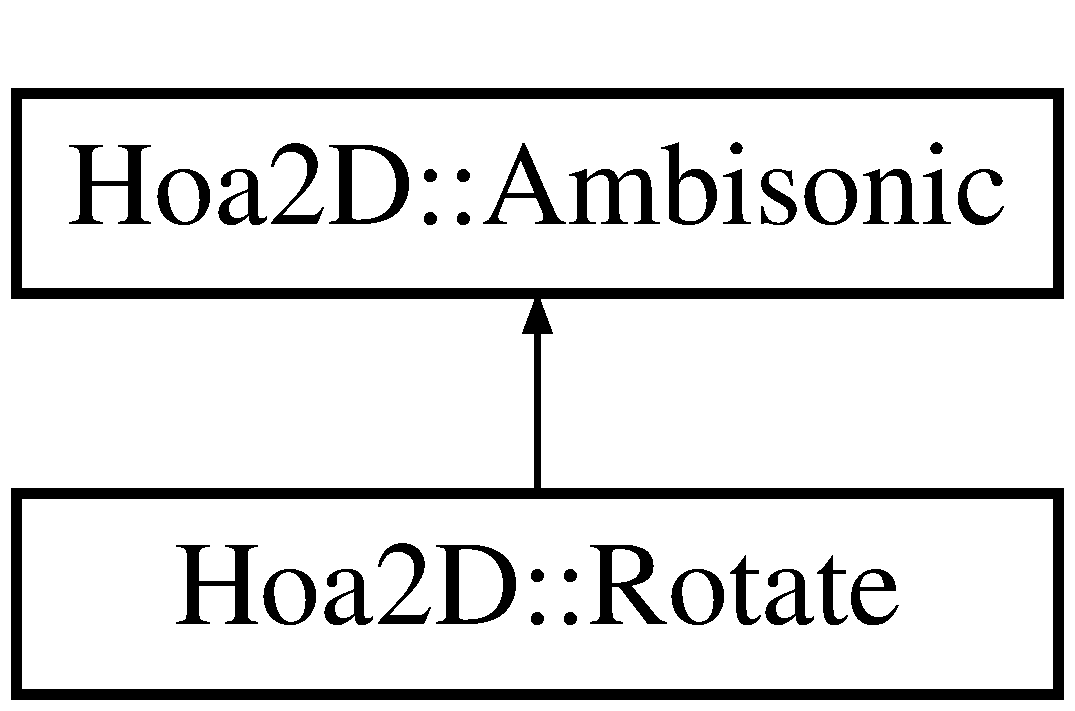
\includegraphics[height=2.000000cm]{class_hoa2_d_1_1_rotate}
\end{center}
\end{figure}
\subsection*{Public Member Functions}
\begin{DoxyCompactItemize}
\item 
\hyperlink{class_hoa2_d_1_1_rotate_a2aa145bb455c0538ce2ca2bd058d8800}{Rotate} (unsigned int order)
\begin{DoxyCompactList}\small\item\em The rotate constructor. \end{DoxyCompactList}\item 
\hyperlink{class_hoa2_d_1_1_rotate_a7e70e8d9099c1b8a2a42313e464130b2}{$\sim$\-Rotate} ()
\begin{DoxyCompactList}\small\item\em The \hyperlink{class_hoa2_d_1_1_rotate}{Rotate} destructor. \end{DoxyCompactList}\item 
void \hyperlink{class_hoa2_d_1_1_rotate_abc51eceaf32e9844d829a816094f6ac5}{set\-Yaw} (const double value)
\begin{DoxyCompactList}\small\item\em This method sets the angle of the rotation around the z axis, the yaw value,. \end{DoxyCompactList}\item 
double \hyperlink{class_hoa2_d_1_1_rotate_a5f40eff256bd5b845d6b4cfc046cd84e}{get\-Yaw} () const 
\begin{DoxyCompactList}\small\item\em Get the angle of the rotation around the z axis, the yaw value. \end{DoxyCompactList}\item 
void \hyperlink{class_hoa2_d_1_1_rotate_a88bfa68435d940b0c4c1ae0c97baeffd}{process} (const float $\ast$inputs, float $\ast$outputs)
\begin{DoxyCompactList}\small\item\em This method performs the rotation with single precision. \end{DoxyCompactList}\item 
void \hyperlink{class_hoa2_d_1_1_rotate_a8d5ecedca52ad2216efe218b5dcbf834}{process} (const double $\ast$inputs, double $\ast$outputs)
\begin{DoxyCompactList}\small\item\em This method performs the rotation with double precision. \end{DoxyCompactList}\end{DoxyCompactItemize}


\subsection{Detailed Description}
The ambisonic rotation. 

The rotate should be used to rotate the ambisonic soundfield. 

Definition at line 17 of file Rotate.\-h.



\subsection{Constructor \& Destructor Documentation}
\hypertarget{class_hoa2_d_1_1_rotate_a2aa145bb455c0538ce2ca2bd058d8800}{\index{Hoa2\-D\-::\-Rotate@{Hoa2\-D\-::\-Rotate}!Rotate@{Rotate}}
\index{Rotate@{Rotate}!Hoa2D::Rotate@{Hoa2\-D\-::\-Rotate}}
\subsubsection[{Rotate}]{\setlength{\rightskip}{0pt plus 5cm}Hoa2\-D\-::\-Rotate\-::\-Rotate (
\begin{DoxyParamCaption}
\item[{unsigned int}]{order}
\end{DoxyParamCaption}
)}}\label{class_hoa2_d_1_1_rotate_a2aa145bb455c0538ce2ca2bd058d8800}


The rotate constructor. 

The rotate constructor allocates and initialize the member values to computes spherical harmonics rotation depending on a decomposition order. The order must be at least 1.


\begin{DoxyParams}{Parameters}
{\em order} & The order. \\
\hline
\end{DoxyParams}


Definition at line 11 of file Rotate.\-cpp.

\hypertarget{class_hoa2_d_1_1_rotate_a7e70e8d9099c1b8a2a42313e464130b2}{\index{Hoa2\-D\-::\-Rotate@{Hoa2\-D\-::\-Rotate}!$\sim$\-Rotate@{$\sim$\-Rotate}}
\index{$\sim$\-Rotate@{$\sim$\-Rotate}!Hoa2D::Rotate@{Hoa2\-D\-::\-Rotate}}
\subsubsection[{$\sim$\-Rotate}]{\setlength{\rightskip}{0pt plus 5cm}Hoa2\-D\-::\-Rotate\-::$\sim$\-Rotate (
\begin{DoxyParamCaption}
{}
\end{DoxyParamCaption}
)}}\label{class_hoa2_d_1_1_rotate_a7e70e8d9099c1b8a2a42313e464130b2}


The \hyperlink{class_hoa2_d_1_1_rotate}{Rotate} destructor. 

The \hyperlink{class_hoa2_d_1_1_rotate}{Rotate} destructor free the memory. 

Definition at line 59 of file Rotate.\-cpp.



\subsection{Member Function Documentation}
\hypertarget{class_hoa2_d_1_1_rotate_a5f40eff256bd5b845d6b4cfc046cd84e}{\index{Hoa2\-D\-::\-Rotate@{Hoa2\-D\-::\-Rotate}!get\-Yaw@{get\-Yaw}}
\index{get\-Yaw@{get\-Yaw}!Hoa2D::Rotate@{Hoa2\-D\-::\-Rotate}}
\subsubsection[{get\-Yaw}]{\setlength{\rightskip}{0pt plus 5cm}double Hoa2\-D\-::\-Rotate\-::get\-Yaw (
\begin{DoxyParamCaption}
{}
\end{DoxyParamCaption}
) const\hspace{0.3cm}{\ttfamily [inline]}}}\label{class_hoa2_d_1_1_rotate_a5f40eff256bd5b845d6b4cfc046cd84e}


Get the angle of the rotation around the z axis, the yaw value. 

The method returns the angle of the rotation around the z axis, the yaw value, in radian between 0 and 2π.

\begin{DoxyReturn}{Returns}
The yaw value. 
\end{DoxyReturn}


Definition at line 51 of file Rotate.\-h.

\hypertarget{class_hoa2_d_1_1_rotate_a88bfa68435d940b0c4c1ae0c97baeffd}{\index{Hoa2\-D\-::\-Rotate@{Hoa2\-D\-::\-Rotate}!process@{process}}
\index{process@{process}!Hoa2D::Rotate@{Hoa2\-D\-::\-Rotate}}
\subsubsection[{process}]{\setlength{\rightskip}{0pt plus 5cm}void Hoa2\-D\-::\-Rotate\-::process (
\begin{DoxyParamCaption}
\item[{const float $\ast$}]{inputs, }
\item[{float $\ast$}]{outputs}
\end{DoxyParamCaption}
)}}\label{class_hoa2_d_1_1_rotate_a88bfa68435d940b0c4c1ae0c97baeffd}


This method performs the rotation with single precision. 

You should use this method for in-\/place or not-\/in-\/place processing and performs the rotation sample by sample. The inputs array and outputs array contains the spherical harmonics samples and the minimum size must be the number of harmonics.


\begin{DoxyParams}{Parameters}
{\em inputs} & The input array. \\
\hline
{\em outputs} & The output array. \\
\hline
\end{DoxyParams}


Definition at line 23 of file Rotate.\-cpp.

\hypertarget{class_hoa2_d_1_1_rotate_a8d5ecedca52ad2216efe218b5dcbf834}{\index{Hoa2\-D\-::\-Rotate@{Hoa2\-D\-::\-Rotate}!process@{process}}
\index{process@{process}!Hoa2D::Rotate@{Hoa2\-D\-::\-Rotate}}
\subsubsection[{process}]{\setlength{\rightskip}{0pt plus 5cm}void Hoa2\-D\-::\-Rotate\-::process (
\begin{DoxyParamCaption}
\item[{const double $\ast$}]{inputs, }
\item[{double $\ast$}]{outputs}
\end{DoxyParamCaption}
)}}\label{class_hoa2_d_1_1_rotate_a8d5ecedca52ad2216efe218b5dcbf834}


This method performs the rotation with double precision. 

You should use this method for in-\/place or not-\/in-\/place processing and performs the rotation sample by sample. The inputs array and outputs array contains the spherical harmonics samples and the minimum size must be the number of harmonics.


\begin{DoxyParams}{Parameters}
{\em inputs} & The input array. \\
\hline
{\em outputs} & The output array. \\
\hline
\end{DoxyParams}


Definition at line 41 of file Rotate.\-cpp.

\hypertarget{class_hoa2_d_1_1_rotate_abc51eceaf32e9844d829a816094f6ac5}{\index{Hoa2\-D\-::\-Rotate@{Hoa2\-D\-::\-Rotate}!set\-Yaw@{set\-Yaw}}
\index{set\-Yaw@{set\-Yaw}!Hoa2D::Rotate@{Hoa2\-D\-::\-Rotate}}
\subsubsection[{set\-Yaw}]{\setlength{\rightskip}{0pt plus 5cm}void Hoa2\-D\-::\-Rotate\-::set\-Yaw (
\begin{DoxyParamCaption}
\item[{const double}]{value}
\end{DoxyParamCaption}
)}}\label{class_hoa2_d_1_1_rotate_abc51eceaf32e9844d829a816094f6ac5}


This method sets the angle of the rotation around the z axis, the yaw value,. 

The yaw is equivalent to a rotation around the z axis, the value is in radian and should be between 0 and 2π.


\begin{DoxyParams}{Parameters}
{\em value} & The yaw value. \\
\hline
\end{DoxyParams}


Definition at line 16 of file Rotate.\-cpp.



The documentation for this class was generated from the following files\-:\begin{DoxyCompactItemize}
\item 
/\-Users/elioton/\-Documents/programmation/\-C\-I\-C\-M/source\-Tree/\-Hoa\-Library/\-Sources/\-Hoa2\-D/Rotate.\-h\item 
/\-Users/elioton/\-Documents/programmation/\-C\-I\-C\-M/source\-Tree/\-Hoa\-Library/\-Sources/\-Hoa2\-D/Rotate.\-cpp\end{DoxyCompactItemize}

\hypertarget{class_hoa3_d_1_1_rotate}{\section{Hoa3\-D\-:\-:Rotate Class Reference}
\label{class_hoa3_d_1_1_rotate}\index{Hoa3\-D\-::\-Rotate@{Hoa3\-D\-::\-Rotate}}
}


The ambisonic \hyperlink{class_hoa3_d_1_1_rotate}{Rotate}.  




{\ttfamily \#include $<$Rotate.\-h$>$}

Inheritance diagram for Hoa3\-D\-:\-:Rotate\-:\begin{figure}[H]
\begin{center}
\leavevmode
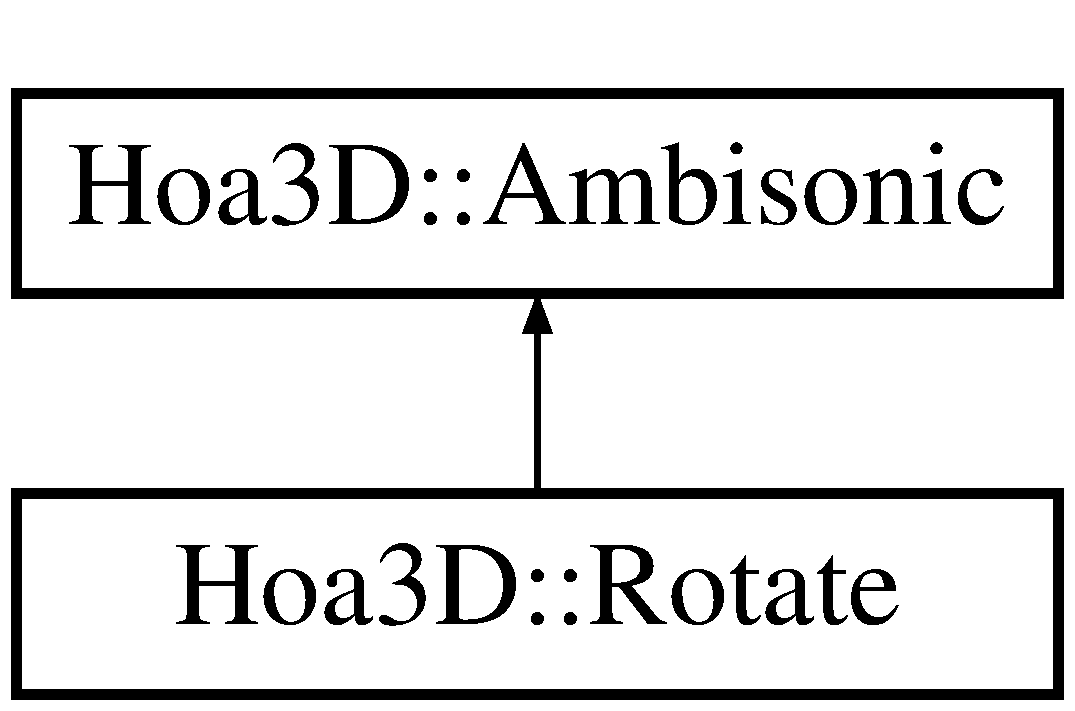
\includegraphics[height=2.000000cm]{class_hoa3_d_1_1_rotate}
\end{center}
\end{figure}
\subsection*{Public Member Functions}
\begin{DoxyCompactItemize}
\item 
\hyperlink{class_hoa3_d_1_1_rotate_a9a5750cbff8e0449b3de62e7de338a8b}{Rotate} (unsigned int order)
\begin{DoxyCompactList}\small\item\em The \hyperlink{class_hoa3_d_1_1_rotate}{Rotate} constructor. \end{DoxyCompactList}\item 
\hyperlink{class_hoa3_d_1_1_rotate_a13a37adfe31314b7d5844333a4e587ab}{$\sim$\-Rotate} ()
\begin{DoxyCompactList}\small\item\em The \hyperlink{class_hoa3_d_1_1_rotate}{Rotate} destructor. \end{DoxyCompactList}\item 
void \hyperlink{class_hoa3_d_1_1_rotate_a190ffb26419c5ab6c7935d48e9a7e23b}{set\-Rotations} (const double roll, const double pitch, const double yaw)
\begin{DoxyCompactList}\small\item\em This method sets the three rotation values at the same time (xyz axis). \end{DoxyCompactList}\item 
void \hyperlink{class_hoa3_d_1_1_rotate_a89599a9cd8c10240ce71b8fd7bdbb3b7}{set\-Roll} (const double value)
\begin{DoxyCompactList}\small\item\em This method sets the roll value (rotation on the x-\/axis). \end{DoxyCompactList}\item 
void \hyperlink{class_hoa3_d_1_1_rotate_aeb7e844c29c2f9bb9cc7de3ef89385f6}{set\-Pitch} (const double value)
\begin{DoxyCompactList}\small\item\em This method sets the pitch value (rotation on the y-\/axis). \end{DoxyCompactList}\item 
void \hyperlink{class_hoa3_d_1_1_rotate_a18df4eaec4e8c7c60f8234632af06d6f}{set\-Yaw} (const double value)
\begin{DoxyCompactList}\small\item\em This method sets the yaw value (rotation on the z-\/axis). \end{DoxyCompactList}\item 
double \hyperlink{class_hoa3_d_1_1_rotate_a4da29df01f2c7311490df11d4322b5f8}{get\-Roll} () const 
\begin{DoxyCompactList}\small\item\em Get the roll value (rotation on the x-\/axis). \end{DoxyCompactList}\item 
double \hyperlink{class_hoa3_d_1_1_rotate_afe1e5ccea5d375b082b7df2b8c8b972a}{get\-Pitch} () const 
\begin{DoxyCompactList}\small\item\em Get the pitch value (rotation on the y-\/axis). \end{DoxyCompactList}\item 
double \hyperlink{class_hoa3_d_1_1_rotate_a386f1fba4ceab4c2e243b7a222124d7e}{get\-Yaw} () const 
\begin{DoxyCompactList}\small\item\em Get the yaw value (rotation on the z-\/axis). \end{DoxyCompactList}\item 
void \hyperlink{class_hoa3_d_1_1_rotate_a9851055e9dbe808578e435c65f22c06a}{process} (const float $\ast$inputs, float $\ast$outputs)
\begin{DoxyCompactList}\small\item\em This method performs the rotation with single precision. \end{DoxyCompactList}\item 
void \hyperlink{class_hoa3_d_1_1_rotate_a395dafa6cc2d92562e6ac8044a438b2c}{process} (const double $\ast$inputs, double $\ast$outputs)
\begin{DoxyCompactList}\small\item\em This method performs the rotation with double precision. \end{DoxyCompactList}\end{DoxyCompactItemize}


\subsection{Detailed Description}
The ambisonic \hyperlink{class_hoa3_d_1_1_rotate}{Rotate}. 

The \hyperlink{class_hoa3_d_1_1_rotate}{Rotate} should be used to rotate an entire soundfield. 

Definition at line 18 of file Rotate.\-h.



\subsection{Constructor \& Destructor Documentation}
\hypertarget{class_hoa3_d_1_1_rotate_a9a5750cbff8e0449b3de62e7de338a8b}{\index{Hoa3\-D\-::\-Rotate@{Hoa3\-D\-::\-Rotate}!Rotate@{Rotate}}
\index{Rotate@{Rotate}!Hoa3D::Rotate@{Hoa3\-D\-::\-Rotate}}
\subsubsection[{Rotate}]{\setlength{\rightskip}{0pt plus 5cm}Hoa3\-D\-::\-Rotate\-::\-Rotate (
\begin{DoxyParamCaption}
\item[{unsigned int}]{order}
\end{DoxyParamCaption}
)}}\label{class_hoa3_d_1_1_rotate_a9a5750cbff8e0449b3de62e7de338a8b}


The \hyperlink{class_hoa3_d_1_1_rotate}{Rotate} constructor. 

The \hyperlink{class_hoa3_d_1_1_rotate}{Rotate} constructor allocates and initialize the member values to computes spherical harmonics rotation depending on a decomposition order. The order must be at least 1.


\begin{DoxyParams}{Parameters}
{\em order} & The order. \\
\hline
\end{DoxyParams}


Definition at line 11 of file Rotate.\-cpp.

\hypertarget{class_hoa3_d_1_1_rotate_a13a37adfe31314b7d5844333a4e587ab}{\index{Hoa3\-D\-::\-Rotate@{Hoa3\-D\-::\-Rotate}!$\sim$\-Rotate@{$\sim$\-Rotate}}
\index{$\sim$\-Rotate@{$\sim$\-Rotate}!Hoa3D::Rotate@{Hoa3\-D\-::\-Rotate}}
\subsubsection[{$\sim$\-Rotate}]{\setlength{\rightskip}{0pt plus 5cm}Hoa3\-D\-::\-Rotate\-::$\sim$\-Rotate (
\begin{DoxyParamCaption}
{}
\end{DoxyParamCaption}
)}}\label{class_hoa3_d_1_1_rotate_a13a37adfe31314b7d5844333a4e587ab}


The \hyperlink{class_hoa3_d_1_1_rotate}{Rotate} destructor. 

The \hyperlink{class_hoa3_d_1_1_rotate}{Rotate} destructor free the memory. 

Definition at line 85 of file Rotate.\-cpp.



\subsection{Member Function Documentation}
\hypertarget{class_hoa3_d_1_1_rotate_afe1e5ccea5d375b082b7df2b8c8b972a}{\index{Hoa3\-D\-::\-Rotate@{Hoa3\-D\-::\-Rotate}!get\-Pitch@{get\-Pitch}}
\index{get\-Pitch@{get\-Pitch}!Hoa3D::Rotate@{Hoa3\-D\-::\-Rotate}}
\subsubsection[{get\-Pitch}]{\setlength{\rightskip}{0pt plus 5cm}double Hoa3\-D\-::\-Rotate\-::get\-Pitch (
\begin{DoxyParamCaption}
{}
\end{DoxyParamCaption}
) const\hspace{0.3cm}{\ttfamily [inline]}}}\label{class_hoa3_d_1_1_rotate_afe1e5ccea5d375b082b7df2b8c8b972a}


Get the pitch value (rotation on the y-\/axis). 

The pitch is equivalent to a rotation on the y-\/axis (also named tumble).

\begin{DoxyReturn}{Returns}
value The pitch value between 0 and 2π. 
\end{DoxyReturn}


Definition at line 94 of file Rotate.\-h.

\hypertarget{class_hoa3_d_1_1_rotate_a4da29df01f2c7311490df11d4322b5f8}{\index{Hoa3\-D\-::\-Rotate@{Hoa3\-D\-::\-Rotate}!get\-Roll@{get\-Roll}}
\index{get\-Roll@{get\-Roll}!Hoa3D::Rotate@{Hoa3\-D\-::\-Rotate}}
\subsubsection[{get\-Roll}]{\setlength{\rightskip}{0pt plus 5cm}double Hoa3\-D\-::\-Rotate\-::get\-Roll (
\begin{DoxyParamCaption}
{}
\end{DoxyParamCaption}
) const\hspace{0.3cm}{\ttfamily [inline]}}}\label{class_hoa3_d_1_1_rotate_a4da29df01f2c7311490df11d4322b5f8}


Get the roll value (rotation on the x-\/axis). 

The roll is equivalent to a rotation on the x-\/axis (also named tilt).

\begin{DoxyReturn}{Returns}
value The roll value between 0 and 2π. 
\end{DoxyReturn}


Definition at line 87 of file Rotate.\-h.

\hypertarget{class_hoa3_d_1_1_rotate_a386f1fba4ceab4c2e243b7a222124d7e}{\index{Hoa3\-D\-::\-Rotate@{Hoa3\-D\-::\-Rotate}!get\-Yaw@{get\-Yaw}}
\index{get\-Yaw@{get\-Yaw}!Hoa3D::Rotate@{Hoa3\-D\-::\-Rotate}}
\subsubsection[{get\-Yaw}]{\setlength{\rightskip}{0pt plus 5cm}double Hoa3\-D\-::\-Rotate\-::get\-Yaw (
\begin{DoxyParamCaption}
{}
\end{DoxyParamCaption}
) const\hspace{0.3cm}{\ttfamily [inline]}}}\label{class_hoa3_d_1_1_rotate_a386f1fba4ceab4c2e243b7a222124d7e}


Get the yaw value (rotation on the z-\/axis). 

The yaw is equivalent to a rotation on the z-\/axis (also named rotation).

\begin{DoxyReturn}{Returns}
value The yaw value between 0 and 2π. 
\end{DoxyReturn}


Definition at line 101 of file Rotate.\-h.

\hypertarget{class_hoa3_d_1_1_rotate_a9851055e9dbe808578e435c65f22c06a}{\index{Hoa3\-D\-::\-Rotate@{Hoa3\-D\-::\-Rotate}!process@{process}}
\index{process@{process}!Hoa3D::Rotate@{Hoa3\-D\-::\-Rotate}}
\subsubsection[{process}]{\setlength{\rightskip}{0pt plus 5cm}void Hoa3\-D\-::\-Rotate\-::process (
\begin{DoxyParamCaption}
\item[{const float $\ast$}]{inputs, }
\item[{float $\ast$}]{outputs}
\end{DoxyParamCaption}
)}}\label{class_hoa3_d_1_1_rotate_a9851055e9dbe808578e435c65f22c06a}


This method performs the rotation with single precision. 

You should use this method for not-\/in-\/place processing and performs the rotation sample by sample. (warning \-: doesn't work with in-\/place vectors); The inputs array and outputs array contains the spherical harmonics samples and the minimum size must be the number of harmonics.


\begin{DoxyParams}{Parameters}
{\em inputs} & The input array. \\
\hline
{\em outputs} & The output array. \\
\hline
\end{DoxyParams}


Definition at line 47 of file Rotate.\-cpp.

\hypertarget{class_hoa3_d_1_1_rotate_a395dafa6cc2d92562e6ac8044a438b2c}{\index{Hoa3\-D\-::\-Rotate@{Hoa3\-D\-::\-Rotate}!process@{process}}
\index{process@{process}!Hoa3D::Rotate@{Hoa3\-D\-::\-Rotate}}
\subsubsection[{process}]{\setlength{\rightskip}{0pt plus 5cm}void Hoa3\-D\-::\-Rotate\-::process (
\begin{DoxyParamCaption}
\item[{const double $\ast$}]{inputs, }
\item[{double $\ast$}]{outputs}
\end{DoxyParamCaption}
)}}\label{class_hoa3_d_1_1_rotate_a395dafa6cc2d92562e6ac8044a438b2c}


This method performs the rotation with double precision. 

You should use this method for not-\/in-\/place processing and performs the rotation sample by sample. (warning \-: doesn't work with in-\/place vectors); The inputs array and outputs array contains the spherical harmonics samples and the minimum size must be the number of harmonics.


\begin{DoxyParams}{Parameters}
{\em inputs} & The input array. \\
\hline
{\em outputs} & The output array. \\
\hline
\end{DoxyParams}


Definition at line 53 of file Rotate.\-cpp.

\hypertarget{class_hoa3_d_1_1_rotate_aeb7e844c29c2f9bb9cc7de3ef89385f6}{\index{Hoa3\-D\-::\-Rotate@{Hoa3\-D\-::\-Rotate}!set\-Pitch@{set\-Pitch}}
\index{set\-Pitch@{set\-Pitch}!Hoa3D::Rotate@{Hoa3\-D\-::\-Rotate}}
\subsubsection[{set\-Pitch}]{\setlength{\rightskip}{0pt plus 5cm}void Hoa3\-D\-::\-Rotate\-::set\-Pitch (
\begin{DoxyParamCaption}
\item[{const double}]{value}
\end{DoxyParamCaption}
)}}\label{class_hoa3_d_1_1_rotate_aeb7e844c29c2f9bb9cc7de3ef89385f6}


This method sets the pitch value (rotation on the y-\/axis). 

The pitch is equivalent to a rotation on the y-\/axis (also named tumble).


\begin{DoxyParams}{Parameters}
{\em value} & The pitch value between 0 and 2π. \\
\hline
\end{DoxyParams}


Definition at line 34 of file Rotate.\-cpp.

\hypertarget{class_hoa3_d_1_1_rotate_a89599a9cd8c10240ce71b8fd7bdbb3b7}{\index{Hoa3\-D\-::\-Rotate@{Hoa3\-D\-::\-Rotate}!set\-Roll@{set\-Roll}}
\index{set\-Roll@{set\-Roll}!Hoa3D::Rotate@{Hoa3\-D\-::\-Rotate}}
\subsubsection[{set\-Roll}]{\setlength{\rightskip}{0pt plus 5cm}void Hoa3\-D\-::\-Rotate\-::set\-Roll (
\begin{DoxyParamCaption}
\item[{const double}]{value}
\end{DoxyParamCaption}
)}}\label{class_hoa3_d_1_1_rotate_a89599a9cd8c10240ce71b8fd7bdbb3b7}


This method sets the roll value (rotation on the x-\/axis). 

The roll is equivalent to a rotation on the x-\/axis (also named tilt).


\begin{DoxyParams}{Parameters}
{\em value} & The roll value between 0 and 2π. \\
\hline
\end{DoxyParams}


Definition at line 27 of file Rotate.\-cpp.

\hypertarget{class_hoa3_d_1_1_rotate_a190ffb26419c5ab6c7935d48e9a7e23b}{\index{Hoa3\-D\-::\-Rotate@{Hoa3\-D\-::\-Rotate}!set\-Rotations@{set\-Rotations}}
\index{set\-Rotations@{set\-Rotations}!Hoa3D::Rotate@{Hoa3\-D\-::\-Rotate}}
\subsubsection[{set\-Rotations}]{\setlength{\rightskip}{0pt plus 5cm}void Hoa3\-D\-::\-Rotate\-::set\-Rotations (
\begin{DoxyParamCaption}
\item[{const double}]{roll, }
\item[{const double}]{pitch, }
\item[{const double}]{yaw}
\end{DoxyParamCaption}
)}}\label{class_hoa3_d_1_1_rotate_a190ffb26419c5ab6c7935d48e9a7e23b}


This method sets the three rotation values at the same time (xyz axis). 

This method sets the three rotation values at the same time (xyz axis).


\begin{DoxyParams}{Parameters}
{\em roll} & The roll value is equivalent to a rotation on the x-\/axis (also named tilt), between 0 and 2π. \\
\hline
{\em pitch} & The pitch value is equivalent to a rotation on the y-\/axis (also named tumble), between 0 and 2π. \\
\hline
{\em yaw} & The yaw value is equivalent to a rotation on the z-\/axis (also named rotation), between 0 and 2π. \\
\hline
\end{DoxyParams}
\begin{DoxySeeAlso}{See Also}
\hyperlink{class_hoa3_d_1_1_rotate_a89599a9cd8c10240ce71b8fd7bdbb3b7}{set\-Roll}, \hyperlink{class_hoa3_d_1_1_rotate_aeb7e844c29c2f9bb9cc7de3ef89385f6}{set\-Pitch}, \hyperlink{class_hoa3_d_1_1_rotate_a18df4eaec4e8c7c60f8234632af06d6f}{set\-Yaw} 
\end{DoxySeeAlso}


Definition at line 20 of file Rotate.\-cpp.

\hypertarget{class_hoa3_d_1_1_rotate_a18df4eaec4e8c7c60f8234632af06d6f}{\index{Hoa3\-D\-::\-Rotate@{Hoa3\-D\-::\-Rotate}!set\-Yaw@{set\-Yaw}}
\index{set\-Yaw@{set\-Yaw}!Hoa3D::Rotate@{Hoa3\-D\-::\-Rotate}}
\subsubsection[{set\-Yaw}]{\setlength{\rightskip}{0pt plus 5cm}void Hoa3\-D\-::\-Rotate\-::set\-Yaw (
\begin{DoxyParamCaption}
\item[{const double}]{value}
\end{DoxyParamCaption}
)}}\label{class_hoa3_d_1_1_rotate_a18df4eaec4e8c7c60f8234632af06d6f}


This method sets the yaw value (rotation on the z-\/axis). 

The yaw is equivalent to a rotation on the z-\/axis (also named rotation).


\begin{DoxyParams}{Parameters}
{\em value} & The yaw value between 0 and 2π. \\
\hline
\end{DoxyParams}


Definition at line 39 of file Rotate.\-cpp.



The documentation for this class was generated from the following files\-:\begin{DoxyCompactItemize}
\item 
/\-Users/elioton/\-Documents/programmation/\-C\-I\-C\-M/source\-Tree/\-Hoa\-Library/\-Sources/\-Hoa3\-D/Rotate.\-h\item 
/\-Users/elioton/\-Documents/programmation/\-C\-I\-C\-M/source\-Tree/\-Hoa\-Library/\-Sources/\-Hoa3\-D/Rotate.\-cpp\end{DoxyCompactItemize}

\hypertarget{class_hoa2_d_1_1_scope}{\section{Hoa2\-D\-:\-:Scope Class Reference}
\label{class_hoa2_d_1_1_scope}\index{Hoa2\-D\-::\-Scope@{Hoa2\-D\-::\-Scope}}
}


The ambisonic scope.  




{\ttfamily \#include $<$Scope.\-h$>$}

Inheritance diagram for Hoa2\-D\-:\-:Scope\-:\begin{figure}[H]
\begin{center}
\leavevmode
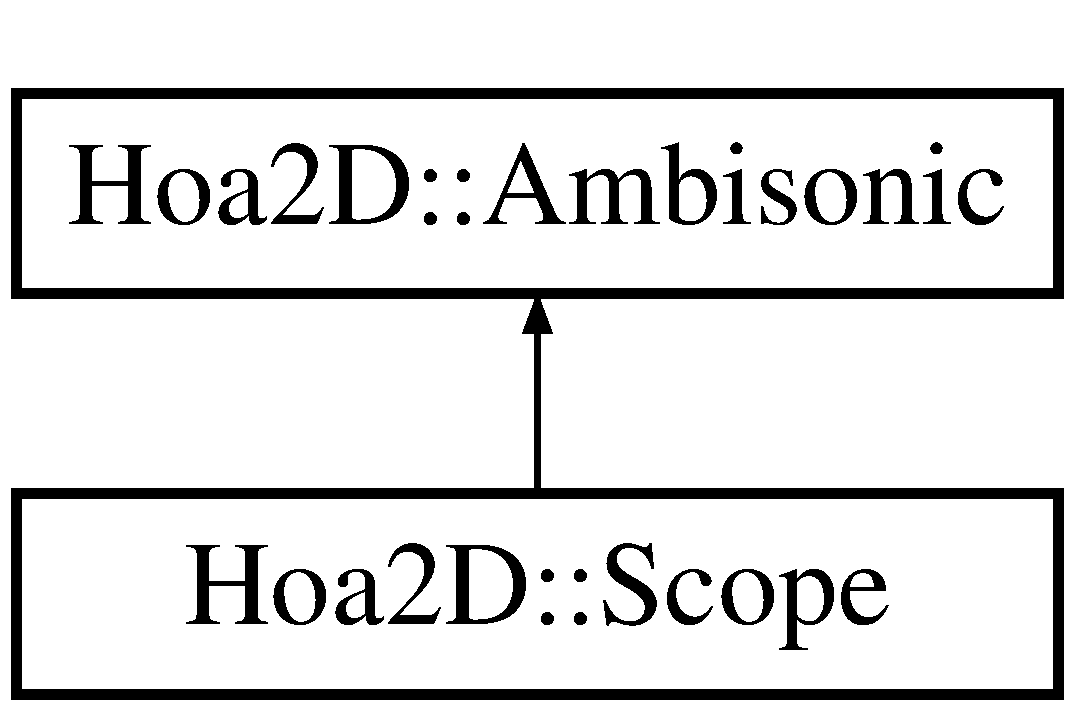
\includegraphics[height=2.000000cm]{class_hoa2_d_1_1_scope}
\end{center}
\end{figure}
\subsection*{Public Member Functions}
\begin{DoxyCompactItemize}
\item 
\hyperlink{class_hoa2_d_1_1_scope_aaa6b3e208eb06bef06b59264c84a5364}{Scope} (unsigned int order, unsigned int number\-Of\-Points)
\begin{DoxyCompactList}\small\item\em The scope constructor. \end{DoxyCompactList}\item 
\hyperlink{class_hoa2_d_1_1_scope_a29c9191706ff1377efab0720cacbc448}{$\sim$\-Scope} ()
\begin{DoxyCompactList}\small\item\em The \hyperlink{class_hoa2_d_1_1_scope}{Scope} destructor. \end{DoxyCompactList}\item 
unsigned int \hyperlink{class_hoa2_d_1_1_scope_adfabc2c966855a3b79a818a503655591}{get\-Number\-Of\-Points} () const 
\begin{DoxyCompactList}\small\item\em Retrieve the number of points. \end{DoxyCompactList}\item 
double \hyperlink{class_hoa2_d_1_1_scope_a69f278dc5e8b40c0f58f6e684078d6eb}{get\-Value} (unsigned int point\-Index) const 
\begin{DoxyCompactList}\small\item\em Retrieve the value of a point of the circular harmonics projection. \end{DoxyCompactList}\item 
double \hyperlink{class_hoa2_d_1_1_scope_a552af7083cc302db946910f68f928f62}{get\-Radius} (unsigned int point\-Index) const 
\begin{DoxyCompactList}\small\item\em Retrieve the radius of a point of the circular harmonics projection. \end{DoxyCompactList}\item 
double \hyperlink{class_hoa2_d_1_1_scope_aa7fff00ef13e8be9c9cd0774301ed258}{get\-Azimuth} (unsigned int point\-Index) const 
\begin{DoxyCompactList}\small\item\em Retrieve the azimuth of a point of the circular harmonics projection. \end{DoxyCompactList}\item 
double \hyperlink{class_hoa2_d_1_1_scope_a80ed96d8739e5ceed58b5b696cd74a24}{get\-Abscissa} (unsigned int point\-Index) const 
\begin{DoxyCompactList}\small\item\em Retrieve the abscissa of a point of the circular harmonics projection. \end{DoxyCompactList}\item 
double \hyperlink{class_hoa2_d_1_1_scope_a10b2a1628c57da3d121ed86c73405702}{get\-Ordinate} (unsigned int point\-Index) const 
\begin{DoxyCompactList}\small\item\em Retrieve the ordinate of a point of the circular harmonics projection. \end{DoxyCompactList}\item 
void \hyperlink{class_hoa2_d_1_1_scope_a038059aad5409d02fb511d3443a5cbce}{process} (const float $\ast$inputs)
\begin{DoxyCompactList}\small\item\em This method performs the circular harmonics projection with single precision. \end{DoxyCompactList}\item 
void \hyperlink{class_hoa2_d_1_1_scope_aa3e07e453b32b6a6334a0945bf102f53}{process} (const double $\ast$inputs)
\begin{DoxyCompactList}\small\item\em This method performs the circular harmonics projection with double precision. \end{DoxyCompactList}\end{DoxyCompactItemize}


\subsection{Detailed Description}
The ambisonic scope. 

The scope discretize a circle by a set of point and uses a decoder to project the circular harmonics on it. This class should be used for graphical interfaces outside the digital signal processing if the number of points to discretize the circle is very large. Then you should prefer to record snapshot of the circular harmonics and to call the process method at an interval adapted to a graphical rendering. 

Definition at line 18 of file Scope.\-h.



\subsection{Constructor \& Destructor Documentation}
\hypertarget{class_hoa2_d_1_1_scope_aaa6b3e208eb06bef06b59264c84a5364}{\index{Hoa2\-D\-::\-Scope@{Hoa2\-D\-::\-Scope}!Scope@{Scope}}
\index{Scope@{Scope}!Hoa2D::Scope@{Hoa2\-D\-::\-Scope}}
\subsubsection[{Scope}]{\setlength{\rightskip}{0pt plus 5cm}Hoa2\-D\-::\-Scope\-::\-Scope (
\begin{DoxyParamCaption}
\item[{unsigned int}]{order, }
\item[{unsigned int}]{number\-Of\-Points}
\end{DoxyParamCaption}
)}}\label{class_hoa2_d_1_1_scope_aaa6b3e208eb06bef06b59264c84a5364}


The scope constructor. 

The scope constructor allocates and initialize the member values to computes circular harmonics projection on a circle depending on a decomposition order and a circle discretization. The circle is discretized by the number of points. The order must be at least 1. The number of points and column should be at least 3 (but it's very low).


\begin{DoxyParams}{Parameters}
{\em order} & The order. \\
\hline
{\em number\-Of\-Points} & The number of points. \\
\hline
\end{DoxyParams}


Definition at line 11 of file Scope.\-cpp.

\hypertarget{class_hoa2_d_1_1_scope_a29c9191706ff1377efab0720cacbc448}{\index{Hoa2\-D\-::\-Scope@{Hoa2\-D\-::\-Scope}!$\sim$\-Scope@{$\sim$\-Scope}}
\index{$\sim$\-Scope@{$\sim$\-Scope}!Hoa2D::Scope@{Hoa2\-D\-::\-Scope}}
\subsubsection[{$\sim$\-Scope}]{\setlength{\rightskip}{0pt plus 5cm}Hoa2\-D\-::\-Scope\-::$\sim$\-Scope (
\begin{DoxyParamCaption}
{}
\end{DoxyParamCaption}
)}}\label{class_hoa2_d_1_1_scope_a29c9191706ff1377efab0720cacbc448}


The \hyperlink{class_hoa2_d_1_1_scope}{Scope} destructor. 

The \hyperlink{class_hoa2_d_1_1_scope}{Scope} destructor free the memory. 

Definition at line 50 of file Scope.\-cpp.



\subsection{Member Function Documentation}
\hypertarget{class_hoa2_d_1_1_scope_a80ed96d8739e5ceed58b5b696cd74a24}{\index{Hoa2\-D\-::\-Scope@{Hoa2\-D\-::\-Scope}!get\-Abscissa@{get\-Abscissa}}
\index{get\-Abscissa@{get\-Abscissa}!Hoa2D::Scope@{Hoa2\-D\-::\-Scope}}
\subsubsection[{get\-Abscissa}]{\setlength{\rightskip}{0pt plus 5cm}double Hoa2\-D\-::\-Scope\-::get\-Abscissa (
\begin{DoxyParamCaption}
\item[{unsigned int}]{point\-Index}
\end{DoxyParamCaption}
) const\hspace{0.3cm}{\ttfamily [inline]}}}\label{class_hoa2_d_1_1_scope_a80ed96d8739e5ceed58b5b696cd74a24}


Retrieve the abscissa of a point of the circular harmonics projection. 

Retrieve the abscissa of the circular harmonics projection for a given point defined by an index.\-The maximum index must be the number of points -\/ 1.


\begin{DoxyParams}{Parameters}
{\em point\-Index} & The point index of the point. \\
\hline
\end{DoxyParams}
\begin{DoxyReturn}{Returns}
This method returns the abscissa of a point of the ambisonic circle.
\end{DoxyReturn}
\begin{DoxySeeAlso}{See Also}
\hyperlink{class_hoa2_d_1_1_scope_a10b2a1628c57da3d121ed86c73405702}{get\-Ordinate} 
\end{DoxySeeAlso}


Definition at line 103 of file Scope.\-h.

\hypertarget{class_hoa2_d_1_1_scope_aa7fff00ef13e8be9c9cd0774301ed258}{\index{Hoa2\-D\-::\-Scope@{Hoa2\-D\-::\-Scope}!get\-Azimuth@{get\-Azimuth}}
\index{get\-Azimuth@{get\-Azimuth}!Hoa2D::Scope@{Hoa2\-D\-::\-Scope}}
\subsubsection[{get\-Azimuth}]{\setlength{\rightskip}{0pt plus 5cm}double Hoa2\-D\-::\-Scope\-::get\-Azimuth (
\begin{DoxyParamCaption}
\item[{unsigned int}]{point\-Index}
\end{DoxyParamCaption}
) const\hspace{0.3cm}{\ttfamily [inline]}}}\label{class_hoa2_d_1_1_scope_aa7fff00ef13e8be9c9cd0774301ed258}


Retrieve the azimuth of a point of the circular harmonics projection. 

Retrieve the azimuth of the circular harmonics projection for a given point defined by an index.\-The maximum index must be the number of points -\/ 1.


\begin{DoxyParams}{Parameters}
{\em point\-Index} & The point index of the point. \\
\hline
\end{DoxyParams}
\begin{DoxyReturn}{Returns}
This method returns the azimuth of a point of the ambisonic circle.
\end{DoxyReturn}
\begin{DoxySeeAlso}{See Also}
\hyperlink{class_hoa2_d_1_1_scope_a69f278dc5e8b40c0f58f6e684078d6eb}{get\-Value} 

\hyperlink{class_hoa2_d_1_1_scope_a552af7083cc302db946910f68f928f62}{get\-Radius} 
\end{DoxySeeAlso}


Definition at line 89 of file Scope.\-h.

\hypertarget{class_hoa2_d_1_1_scope_adfabc2c966855a3b79a818a503655591}{\index{Hoa2\-D\-::\-Scope@{Hoa2\-D\-::\-Scope}!get\-Number\-Of\-Points@{get\-Number\-Of\-Points}}
\index{get\-Number\-Of\-Points@{get\-Number\-Of\-Points}!Hoa2D::Scope@{Hoa2\-D\-::\-Scope}}
\subsubsection[{get\-Number\-Of\-Points}]{\setlength{\rightskip}{0pt plus 5cm}unsigned int Hoa2\-D\-::\-Scope\-::get\-Number\-Of\-Points (
\begin{DoxyParamCaption}
{}
\end{DoxyParamCaption}
) const\hspace{0.3cm}{\ttfamily [inline]}}}\label{class_hoa2_d_1_1_scope_adfabc2c966855a3b79a818a503655591}


Retrieve the number of points. 

Retrieve the number of points used to discretize the ambisonic circle.

\begin{DoxyReturn}{Returns}
This method returns the number of points used to discretize the circle. 
\end{DoxyReturn}


Definition at line 45 of file Scope.\-h.

\hypertarget{class_hoa2_d_1_1_scope_a10b2a1628c57da3d121ed86c73405702}{\index{Hoa2\-D\-::\-Scope@{Hoa2\-D\-::\-Scope}!get\-Ordinate@{get\-Ordinate}}
\index{get\-Ordinate@{get\-Ordinate}!Hoa2D::Scope@{Hoa2\-D\-::\-Scope}}
\subsubsection[{get\-Ordinate}]{\setlength{\rightskip}{0pt plus 5cm}double Hoa2\-D\-::\-Scope\-::get\-Ordinate (
\begin{DoxyParamCaption}
\item[{unsigned int}]{point\-Index}
\end{DoxyParamCaption}
) const\hspace{0.3cm}{\ttfamily [inline]}}}\label{class_hoa2_d_1_1_scope_a10b2a1628c57da3d121ed86c73405702}


Retrieve the ordinate of a point of the circular harmonics projection. 

Retrieve the ordinate of the circular harmonics projection for a given point defined by an index.\-The maximum index must be the number of points -\/ 1.


\begin{DoxyParams}{Parameters}
{\em point\-Index} & The point index of the point. \\
\hline
\end{DoxyParams}
\begin{DoxyReturn}{Returns}
This method returns the ordinate of a point of the ambisonic circle.
\end{DoxyReturn}
\begin{DoxySeeAlso}{See Also}
\hyperlink{class_hoa2_d_1_1_scope_a80ed96d8739e5ceed58b5b696cd74a24}{get\-Abscissa} 
\end{DoxySeeAlso}


Definition at line 117 of file Scope.\-h.

\hypertarget{class_hoa2_d_1_1_scope_a552af7083cc302db946910f68f928f62}{\index{Hoa2\-D\-::\-Scope@{Hoa2\-D\-::\-Scope}!get\-Radius@{get\-Radius}}
\index{get\-Radius@{get\-Radius}!Hoa2D::Scope@{Hoa2\-D\-::\-Scope}}
\subsubsection[{get\-Radius}]{\setlength{\rightskip}{0pt plus 5cm}double Hoa2\-D\-::\-Scope\-::get\-Radius (
\begin{DoxyParamCaption}
\item[{unsigned int}]{point\-Index}
\end{DoxyParamCaption}
) const\hspace{0.3cm}{\ttfamily [inline]}}}\label{class_hoa2_d_1_1_scope_a552af7083cc302db946910f68f928f62}


Retrieve the radius of a point of the circular harmonics projection. 

Retrieve the radius of the circular harmonics projection for a given point defined by an index. This the absolute of the result of the projection. For the index, 0 is the 0 azimtuh of the circle. The maximum index must be the number of points -\/ 1.


\begin{DoxyParams}{Parameters}
{\em point\-Index} & The point index of the point. \\
\hline
\end{DoxyParams}
\begin{DoxyReturn}{Returns}
This method returns the radius of a point of the ambisonic circle.
\end{DoxyReturn}
\begin{DoxySeeAlso}{See Also}
\hyperlink{class_hoa2_d_1_1_scope_aa7fff00ef13e8be9c9cd0774301ed258}{get\-Azimuth} 

\hyperlink{class_hoa2_d_1_1_scope_a69f278dc5e8b40c0f58f6e684078d6eb}{get\-Value} 
\end{DoxySeeAlso}


Definition at line 74 of file Scope.\-h.

\hypertarget{class_hoa2_d_1_1_scope_a69f278dc5e8b40c0f58f6e684078d6eb}{\index{Hoa2\-D\-::\-Scope@{Hoa2\-D\-::\-Scope}!get\-Value@{get\-Value}}
\index{get\-Value@{get\-Value}!Hoa2D::Scope@{Hoa2\-D\-::\-Scope}}
\subsubsection[{get\-Value}]{\setlength{\rightskip}{0pt plus 5cm}double Hoa2\-D\-::\-Scope\-::get\-Value (
\begin{DoxyParamCaption}
\item[{unsigned int}]{point\-Index}
\end{DoxyParamCaption}
) const\hspace{0.3cm}{\ttfamily [inline]}}}\label{class_hoa2_d_1_1_scope_a69f278dc5e8b40c0f58f6e684078d6eb}


Retrieve the value of a point of the circular harmonics projection. 

\begin{DoxyVerb}Retrieve the result value of the circular harmonics projection for a given point defined by an index. The absolute of the value can be used as the radius of the point for a 2 dimentionnal representation. For the index, 0 is the 0 azimtuh of the circle. The maximum index must be the number of points - 1.
\end{DoxyVerb}



\begin{DoxyParams}{Parameters}
{\em point\-Index} & The point index of the point. \\
\hline
\end{DoxyParams}
\begin{DoxyReturn}{Returns}
This method returns the value of a point of the ambisonic circle.
\end{DoxyReturn}
\begin{DoxySeeAlso}{See Also}
getradius 

\hyperlink{class_hoa2_d_1_1_scope_aa7fff00ef13e8be9c9cd0774301ed258}{get\-Azimuth} 
\end{DoxySeeAlso}


Definition at line 59 of file Scope.\-h.

\hypertarget{class_hoa2_d_1_1_scope_a038059aad5409d02fb511d3443a5cbce}{\index{Hoa2\-D\-::\-Scope@{Hoa2\-D\-::\-Scope}!process@{process}}
\index{process@{process}!Hoa2D::Scope@{Hoa2\-D\-::\-Scope}}
\subsubsection[{process}]{\setlength{\rightskip}{0pt plus 5cm}void Hoa2\-D\-::\-Scope\-::process (
\begin{DoxyParamCaption}
\item[{const float $\ast$}]{inputs}
\end{DoxyParamCaption}
)}}\label{class_hoa2_d_1_1_scope_a038059aad5409d02fb511d3443a5cbce}


This method performs the circular harmonics projection with single precision. 

You should use this method to compute the projection of the circular harmonics over an ambisonics circle. The inputs array contains the circular harmonics samples and the minimum size must be the number of harmonics.


\begin{DoxyParams}{Parameters}
{\em inputs} & The inputs array. \\
\hline
\end{DoxyParams}


Definition at line 24 of file Scope.\-cpp.

\hypertarget{class_hoa2_d_1_1_scope_aa3e07e453b32b6a6334a0945bf102f53}{\index{Hoa2\-D\-::\-Scope@{Hoa2\-D\-::\-Scope}!process@{process}}
\index{process@{process}!Hoa2D::Scope@{Hoa2\-D\-::\-Scope}}
\subsubsection[{process}]{\setlength{\rightskip}{0pt plus 5cm}void Hoa2\-D\-::\-Scope\-::process (
\begin{DoxyParamCaption}
\item[{const double $\ast$}]{inputs}
\end{DoxyParamCaption}
)}}\label{class_hoa2_d_1_1_scope_aa3e07e453b32b6a6334a0945bf102f53}


This method performs the circular harmonics projection with double precision. 

You should use this method to compute the projection of the circular harmonics over an ambisonics circle. The inputs array contains the circular harmonics samples and the minimum size must be the number of harmonics.


\begin{DoxyParams}{Parameters}
{\em inputs} & The inputs array. \\
\hline
\end{DoxyParams}


Definition at line 39 of file Scope.\-cpp.



The documentation for this class was generated from the following files\-:\begin{DoxyCompactItemize}
\item 
/\-Users/\-Pierre/\-Source\-Tree/\-Hoa\-Library/\-Sources/\-Hoa2\-D/Scope.\-h\item 
/\-Users/\-Pierre/\-Source\-Tree/\-Hoa\-Library/\-Sources/\-Hoa2\-D/Scope.\-cpp\end{DoxyCompactItemize}

\hypertarget{class_hoa3_d_1_1_scope}{\section{Hoa3\-D\-:\-:Scope Class Reference}
\label{class_hoa3_d_1_1_scope}\index{Hoa3\-D\-::\-Scope@{Hoa3\-D\-::\-Scope}}
}


The ambisonic scope.  




{\ttfamily \#include $<$Scope.\-h$>$}

Inheritance diagram for Hoa3\-D\-:\-:Scope\-:\begin{figure}[H]
\begin{center}
\leavevmode
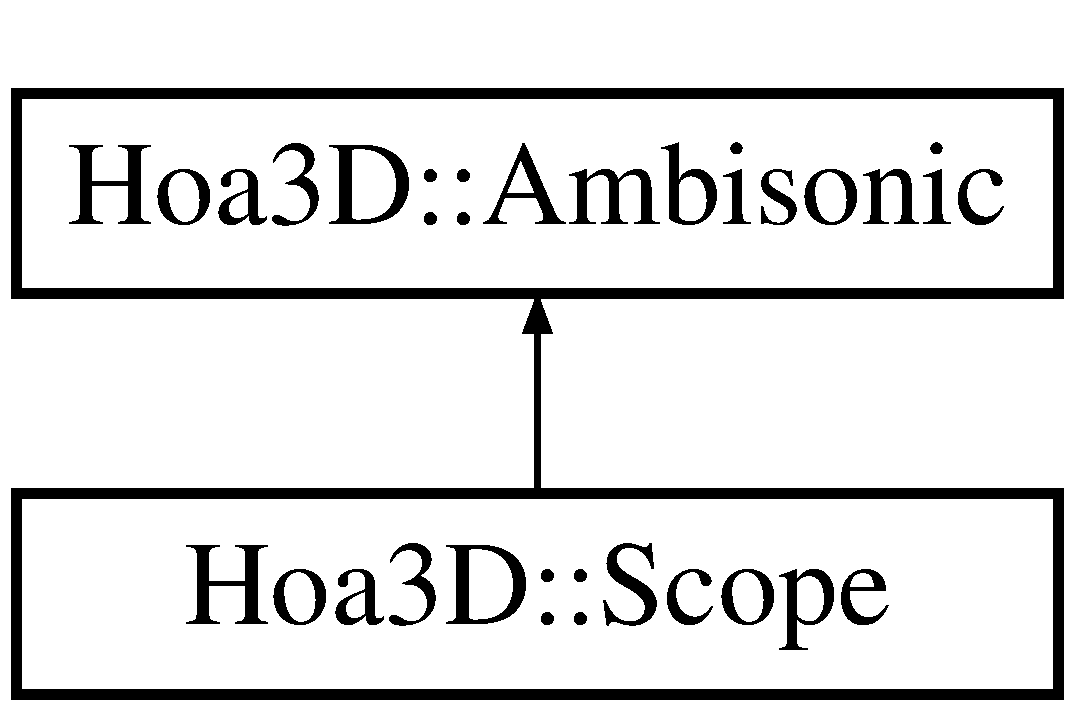
\includegraphics[height=2.000000cm]{class_hoa3_d_1_1_scope}
\end{center}
\end{figure}
\subsection*{Public Member Functions}
\begin{DoxyCompactItemize}
\item 
\hyperlink{class_hoa3_d_1_1_scope_ab4f5ff6674c4df165a1455e4648e1c35}{Scope} (unsigned int order, unsigned int number\-Of\-Rows, unsigned int number\-Of\-Columns)
\begin{DoxyCompactList}\small\item\em The \hyperlink{class_hoa3_d_1_1_scope}{Scope} constructor. \end{DoxyCompactList}\item 
\hyperlink{class_hoa3_d_1_1_scope_a84990cf90c7b3be0963f4cacbdab1df8}{$\sim$\-Scope} ()
\begin{DoxyCompactList}\small\item\em The \hyperlink{class_hoa3_d_1_1_scope}{Scope} destructor. \end{DoxyCompactList}\item 
unsigned int \hyperlink{class_hoa3_d_1_1_scope_aab635359344e855d855972752e6766c9}{get\-Number\-Of\-Rows} () const 
\begin{DoxyCompactList}\small\item\em Retrieve the number of rows. \end{DoxyCompactList}\item 
unsigned int \hyperlink{class_hoa3_d_1_1_scope_abdee40de6953ec537bbc72154ac93e6e}{get\-Number\-Of\-Columns} () const 
\begin{DoxyCompactList}\small\item\em Retrieve the number of column. \end{DoxyCompactList}\item 
double \hyperlink{class_hoa3_d_1_1_scope_a5dd62de174f903097d992da4f108037e}{get\-Value} (unsigned int row\-Index, unsigned int column\-Index) const 
\begin{DoxyCompactList}\small\item\em Retrieve the value of a point of the spherical harmonics projection. \end{DoxyCompactList}\item 
double \hyperlink{class_hoa3_d_1_1_scope_a2452963dd7f2ee7d61af6186d049db24}{get\-Radius} (unsigned int row\-Index, unsigned int column\-Index) const 
\begin{DoxyCompactList}\small\item\em Retrieve the radius of a point of the spherical harmonics projection. \end{DoxyCompactList}\item 
double \hyperlink{class_hoa3_d_1_1_scope_a9a0c8cf80dc5686b746fc3d5b742de45}{get\-Azimuth} (unsigned int column\-Index) const 
\begin{DoxyCompactList}\small\item\em Retrieve the azimuth of a point of the spherical harmonics projection. \end{DoxyCompactList}\item 
double \hyperlink{class_hoa3_d_1_1_scope_ab878f89077b6d2829bf00436aadd309b}{get\-Elevation} (unsigned int row\-Index) const 
\begin{DoxyCompactList}\small\item\em Retrieve the elevation of a point of the spherical harmonics projection. \end{DoxyCompactList}\item 
void \hyperlink{class_hoa3_d_1_1_scope_a4e9866933d1b863860ffd64b0514a6e6}{process} (const float $\ast$inputs)
\begin{DoxyCompactList}\small\item\em This method performs the spherical harmonics projection with single precision. \end{DoxyCompactList}\item 
void \hyperlink{class_hoa3_d_1_1_scope_ae9a788e0352011e3ad7ad5f88b5b12ed}{process} (const double $\ast$inputs)
\begin{DoxyCompactList}\small\item\em This method performs the spherical harmonics projection with double precision. \end{DoxyCompactList}\end{DoxyCompactItemize}


\subsection{Detailed Description}
The ambisonic scope. 

The scope discretize a sphere by a set of point and uses a decoder to project the spherical harmonics on it. This class should be used for graphical interfaces outside the digital signal processing if the number of points to discretize the sphere is very large. Then you should prefer to record snapshot of the spherical harmonics and to call the process method at an interval adapted to a graphical rendering. 

Definition at line 18 of file Scope.\-h.



\subsection{Constructor \& Destructor Documentation}
\hypertarget{class_hoa3_d_1_1_scope_ab4f5ff6674c4df165a1455e4648e1c35}{\index{Hoa3\-D\-::\-Scope@{Hoa3\-D\-::\-Scope}!Scope@{Scope}}
\index{Scope@{Scope}!Hoa3D::Scope@{Hoa3\-D\-::\-Scope}}
\subsubsection[{Scope}]{\setlength{\rightskip}{0pt plus 5cm}Hoa3\-D\-::\-Scope\-::\-Scope (
\begin{DoxyParamCaption}
\item[{unsigned int}]{order, }
\item[{unsigned int}]{number\-Of\-Rows, }
\item[{unsigned int}]{number\-Of\-Columns}
\end{DoxyParamCaption}
)}}\label{class_hoa3_d_1_1_scope_ab4f5ff6674c4df165a1455e4648e1c35}


The \hyperlink{class_hoa3_d_1_1_scope}{Scope} constructor. 

\begin{DoxyVerb}The Scope constructor allocates and initialize the member values to computes spherical harmonics projection on a sphere depending on a decomposition order and a sphere discretization. The sphere discretization is done by a set of points defined by rows and columns then the precision will be lower at the elevation center (0 radian) than at the top (1/2 Pi) or the bottom (-1/2 Pi) of the sphere. The number of row discretize the elevation then it set how many points are used between the bottom and the top. The number of column discretize the azimuth circle then it set how many points are used to make the turn from the front (O radian). Then the sphere is discretized by number of rows * number of columns points. The order must be at least 1. The number of rows and column should be at least 3 (but it's very low).
\end{DoxyVerb}



\begin{DoxyParams}{Parameters}
{\em order} & The order. \\
\hline
{\em number\-Of\-Row} & The number of rows. \\
\hline
{\em number\-Of\-Column} & The number of columns. \\
\hline
\end{DoxyParams}


Definition at line 11 of file Scope.\-cpp.

\hypertarget{class_hoa3_d_1_1_scope_a84990cf90c7b3be0963f4cacbdab1df8}{\index{Hoa3\-D\-::\-Scope@{Hoa3\-D\-::\-Scope}!$\sim$\-Scope@{$\sim$\-Scope}}
\index{$\sim$\-Scope@{$\sim$\-Scope}!Hoa3D::Scope@{Hoa3\-D\-::\-Scope}}
\subsubsection[{$\sim$\-Scope}]{\setlength{\rightskip}{0pt plus 5cm}Hoa3\-D\-::\-Scope\-::$\sim$\-Scope (
\begin{DoxyParamCaption}
{}
\end{DoxyParamCaption}
)}}\label{class_hoa3_d_1_1_scope_a84990cf90c7b3be0963f4cacbdab1df8}


The \hyperlink{class_hoa3_d_1_1_scope}{Scope} destructor. 

The \hyperlink{class_hoa3_d_1_1_scope}{Scope} destructor free the memory. 

Definition at line 54 of file Scope.\-cpp.



\subsection{Member Function Documentation}
\hypertarget{class_hoa3_d_1_1_scope_a9a0c8cf80dc5686b746fc3d5b742de45}{\index{Hoa3\-D\-::\-Scope@{Hoa3\-D\-::\-Scope}!get\-Azimuth@{get\-Azimuth}}
\index{get\-Azimuth@{get\-Azimuth}!Hoa3D::Scope@{Hoa3\-D\-::\-Scope}}
\subsubsection[{get\-Azimuth}]{\setlength{\rightskip}{0pt plus 5cm}double Hoa3\-D\-::\-Scope\-::get\-Azimuth (
\begin{DoxyParamCaption}
\item[{unsigned int}]{column\-Index}
\end{DoxyParamCaption}
) const\hspace{0.3cm}{\ttfamily [inline]}}}\label{class_hoa3_d_1_1_scope_a9a0c8cf80dc5686b746fc3d5b742de45}


Retrieve the azimuth of a point of the spherical harmonics projection. 

\begin{DoxyVerb}Retrieve the azimuth of the spherical harmonics projection for a given point defined by a row index and a column index. For the column index, 0 is the front (0 radian) and number of columns / 2 is the rear of the sphere. The maximum column index must be the number of columns - 1.
\end{DoxyVerb}



\begin{DoxyParams}{Parameters}
{\em row\-Index} & The row index of the point. \\
\hline
{\em column\-Index} & The column index of the point. \\
\hline
\end{DoxyParams}
\begin{DoxyReturn}{Returns}
This method returns the azimuth of a point of the ambisonic sphere. 
\end{DoxyReturn}
\begin{DoxySeeAlso}{See Also}
\hyperlink{class_hoa3_d_1_1_scope_a5dd62de174f903097d992da4f108037e}{get\-Value} 

\hyperlink{class_hoa3_d_1_1_scope_a2452963dd7f2ee7d61af6186d049db24}{get\-Radius} 

\hyperlink{class_hoa3_d_1_1_scope_ab878f89077b6d2829bf00436aadd309b}{get\-Elevation} 
\end{DoxySeeAlso}


Definition at line 106 of file Scope.\-h.

\hypertarget{class_hoa3_d_1_1_scope_ab878f89077b6d2829bf00436aadd309b}{\index{Hoa3\-D\-::\-Scope@{Hoa3\-D\-::\-Scope}!get\-Elevation@{get\-Elevation}}
\index{get\-Elevation@{get\-Elevation}!Hoa3D::Scope@{Hoa3\-D\-::\-Scope}}
\subsubsection[{get\-Elevation}]{\setlength{\rightskip}{0pt plus 5cm}double Hoa3\-D\-::\-Scope\-::get\-Elevation (
\begin{DoxyParamCaption}
\item[{unsigned int}]{row\-Index}
\end{DoxyParamCaption}
) const\hspace{0.3cm}{\ttfamily [inline]}}}\label{class_hoa3_d_1_1_scope_ab878f89077b6d2829bf00436aadd309b}


Retrieve the elevation of a point of the spherical harmonics projection. 

\begin{DoxyVerb}Retrieve the elevation of the spherical harmonics projection for a given point defined by a row index. For the row index, 0 is the bottom of the sphere, number of rows / 2 is at the center of the elevation and number of rows - 1 is at the top of the sphere. The maximum row index must be the number of row - 1.
\end{DoxyVerb}



\begin{DoxyParams}{Parameters}
{\em row\-Index} & The row index of the point. \\
\hline
{\em column\-Index} & The column index of the point. \\
\hline
\end{DoxyParams}
\begin{DoxyReturn}{Returns}
This method returns the elevation of a point of the ambisonic sphere. 
\end{DoxyReturn}
\begin{DoxySeeAlso}{See Also}
\hyperlink{class_hoa3_d_1_1_scope_a5dd62de174f903097d992da4f108037e}{get\-Value} 

\hyperlink{class_hoa3_d_1_1_scope_a2452963dd7f2ee7d61af6186d049db24}{get\-Radius} 

\hyperlink{class_hoa3_d_1_1_scope_a9a0c8cf80dc5686b746fc3d5b742de45}{get\-Azimuth} 
\end{DoxySeeAlso}


Definition at line 122 of file Scope.\-h.

\hypertarget{class_hoa3_d_1_1_scope_abdee40de6953ec537bbc72154ac93e6e}{\index{Hoa3\-D\-::\-Scope@{Hoa3\-D\-::\-Scope}!get\-Number\-Of\-Columns@{get\-Number\-Of\-Columns}}
\index{get\-Number\-Of\-Columns@{get\-Number\-Of\-Columns}!Hoa3D::Scope@{Hoa3\-D\-::\-Scope}}
\subsubsection[{get\-Number\-Of\-Columns}]{\setlength{\rightskip}{0pt plus 5cm}unsigned int Hoa3\-D\-::\-Scope\-::get\-Number\-Of\-Columns (
\begin{DoxyParamCaption}
{}
\end{DoxyParamCaption}
) const\hspace{0.3cm}{\ttfamily [inline]}}}\label{class_hoa3_d_1_1_scope_abdee40de6953ec537bbc72154ac93e6e}


Retrieve the number of column. 

\begin{DoxyVerb}Retrieve the number of column used to discretize the ambisonic sphere.
\end{DoxyVerb}


\begin{DoxyReturn}{Returns}
This method returns the number of column used to discretize the sphere. 
\end{DoxyReturn}


Definition at line 57 of file Scope.\-h.

\hypertarget{class_hoa3_d_1_1_scope_aab635359344e855d855972752e6766c9}{\index{Hoa3\-D\-::\-Scope@{Hoa3\-D\-::\-Scope}!get\-Number\-Of\-Rows@{get\-Number\-Of\-Rows}}
\index{get\-Number\-Of\-Rows@{get\-Number\-Of\-Rows}!Hoa3D::Scope@{Hoa3\-D\-::\-Scope}}
\subsubsection[{get\-Number\-Of\-Rows}]{\setlength{\rightskip}{0pt plus 5cm}unsigned int Hoa3\-D\-::\-Scope\-::get\-Number\-Of\-Rows (
\begin{DoxyParamCaption}
{}
\end{DoxyParamCaption}
) const\hspace{0.3cm}{\ttfamily [inline]}}}\label{class_hoa3_d_1_1_scope_aab635359344e855d855972752e6766c9}


Retrieve the number of rows. 

\begin{DoxyVerb}Retrieve the number of rows used to discretize the ambisonic sphere.
\end{DoxyVerb}


\begin{DoxyReturn}{Returns}
This method returns the number of rows used to discretize the sphere. 
\end{DoxyReturn}


Definition at line 47 of file Scope.\-h.

\hypertarget{class_hoa3_d_1_1_scope_a2452963dd7f2ee7d61af6186d049db24}{\index{Hoa3\-D\-::\-Scope@{Hoa3\-D\-::\-Scope}!get\-Radius@{get\-Radius}}
\index{get\-Radius@{get\-Radius}!Hoa3D::Scope@{Hoa3\-D\-::\-Scope}}
\subsubsection[{get\-Radius}]{\setlength{\rightskip}{0pt plus 5cm}double Hoa3\-D\-::\-Scope\-::get\-Radius (
\begin{DoxyParamCaption}
\item[{unsigned int}]{row\-Index, }
\item[{unsigned int}]{column\-Index}
\end{DoxyParamCaption}
) const\hspace{0.3cm}{\ttfamily [inline]}}}\label{class_hoa3_d_1_1_scope_a2452963dd7f2ee7d61af6186d049db24}


Retrieve the radius of a point of the spherical harmonics projection. 

\begin{DoxyVerb}Retrieve the radius of the spherical harmonics projection for a given point defined by a row index and a column index. This the absolute of the result of the projection. For the row index, 0 is the bottom of the sphere, number of rows / 2 is at the center of the elevation and number of rows - 1 is at the top of the sphere. For the column index, 0 is the front (0 radian) and number of columns / 2 is the rear of the sphere. The maximum row index must be the number of row - 1 and the maximum column index must be the number of columns - 1.
\end{DoxyVerb}



\begin{DoxyParams}{Parameters}
{\em row\-Index} & The row index of the point. \\
\hline
{\em column\-Index} & The column index of the point. \\
\hline
\end{DoxyParams}
\begin{DoxyReturn}{Returns}
This method returns the radius of a point of the ambisonic sphere. 
\end{DoxyReturn}
\begin{DoxySeeAlso}{See Also}
\hyperlink{class_hoa3_d_1_1_scope_a9a0c8cf80dc5686b746fc3d5b742de45}{get\-Azimuth} 

\hyperlink{class_hoa3_d_1_1_scope_ab878f89077b6d2829bf00436aadd309b}{get\-Elevation} 

\hyperlink{class_hoa3_d_1_1_scope_a5dd62de174f903097d992da4f108037e}{get\-Value} 
\end{DoxySeeAlso}


Definition at line 89 of file Scope.\-h.

\hypertarget{class_hoa3_d_1_1_scope_a5dd62de174f903097d992da4f108037e}{\index{Hoa3\-D\-::\-Scope@{Hoa3\-D\-::\-Scope}!get\-Value@{get\-Value}}
\index{get\-Value@{get\-Value}!Hoa3D::Scope@{Hoa3\-D\-::\-Scope}}
\subsubsection[{get\-Value}]{\setlength{\rightskip}{0pt plus 5cm}double Hoa3\-D\-::\-Scope\-::get\-Value (
\begin{DoxyParamCaption}
\item[{unsigned int}]{row\-Index, }
\item[{unsigned int}]{column\-Index}
\end{DoxyParamCaption}
) const\hspace{0.3cm}{\ttfamily [inline]}}}\label{class_hoa3_d_1_1_scope_a5dd62de174f903097d992da4f108037e}


Retrieve the value of a point of the spherical harmonics projection. 

\begin{DoxyVerb}Retrieve the result value of the spherical harmonics projection for a given point defined by a row index and a column index. The absolute of the value can be used as the radius of the point for a 3 dimentionnal representation. For the row index, 0 is the bottom of the sphere, number of rows / 2 is at the center of the elevation and number of rows - 1 is at the top of the sphere. For the column index, 0 is the front (0 radian) and number of columns / 2 is the rear of the sphere. The maximum row index must be the number of row - 1 and the maximum column index must be the number of columns - 1.
\end{DoxyVerb}



\begin{DoxyParams}{Parameters}
{\em row\-Index} & The row index of the point. \\
\hline
{\em column\-Index} & The column index of the point. \\
\hline
\end{DoxyParams}
\begin{DoxyReturn}{Returns}
This method returns the value of a point of the ambisonic sphere. 
\end{DoxyReturn}
\begin{DoxySeeAlso}{See Also}
getradius 

\hyperlink{class_hoa3_d_1_1_scope_a9a0c8cf80dc5686b746fc3d5b742de45}{get\-Azimuth} 

\hyperlink{class_hoa3_d_1_1_scope_ab878f89077b6d2829bf00436aadd309b}{get\-Elevation} 
\end{DoxySeeAlso}


Definition at line 72 of file Scope.\-h.

\hypertarget{class_hoa3_d_1_1_scope_a4e9866933d1b863860ffd64b0514a6e6}{\index{Hoa3\-D\-::\-Scope@{Hoa3\-D\-::\-Scope}!process@{process}}
\index{process@{process}!Hoa3D::Scope@{Hoa3\-D\-::\-Scope}}
\subsubsection[{process}]{\setlength{\rightskip}{0pt plus 5cm}void Hoa3\-D\-::\-Scope\-::process (
\begin{DoxyParamCaption}
\item[{const float $\ast$}]{inputs}
\end{DoxyParamCaption}
)}}\label{class_hoa3_d_1_1_scope_a4e9866933d1b863860ffd64b0514a6e6}


This method performs the spherical harmonics projection with single precision. 

\begin{DoxyVerb}You should use this method to compute the projection of the spherical harmonics over an ambisonics sphere. The inputs array contains the spherical harmonics samples and the minimum size must be the number of harmonics.
\end{DoxyVerb}



\begin{DoxyParams}{Parameters}
{\em inputs} & The inputs array. \\
\hline
\end{DoxyParams}


Definition at line 28 of file Scope.\-cpp.

\hypertarget{class_hoa3_d_1_1_scope_ae9a788e0352011e3ad7ad5f88b5b12ed}{\index{Hoa3\-D\-::\-Scope@{Hoa3\-D\-::\-Scope}!process@{process}}
\index{process@{process}!Hoa3D::Scope@{Hoa3\-D\-::\-Scope}}
\subsubsection[{process}]{\setlength{\rightskip}{0pt plus 5cm}void Hoa3\-D\-::\-Scope\-::process (
\begin{DoxyParamCaption}
\item[{const double $\ast$}]{inputs}
\end{DoxyParamCaption}
)}}\label{class_hoa3_d_1_1_scope_ae9a788e0352011e3ad7ad5f88b5b12ed}


This method performs the spherical harmonics projection with double precision. 

\begin{DoxyVerb}You should use this method to compute the projection of the spherical harmonics over an ambisonics sphere. The inputs array contains the spherical harmonics samples and the minimum size must be the number of harmonics.
\end{DoxyVerb}



\begin{DoxyParams}{Parameters}
{\em inputs} & The inputs array. \\
\hline
\end{DoxyParams}


Definition at line 43 of file Scope.\-cpp.



The documentation for this class was generated from the following files\-:\begin{DoxyCompactItemize}
\item 
/\-Users/\-Pierre/\-Source\-Tree/\-Hoa\-Library/\-Sources/\-Hoa3\-D/Scope.\-h\item 
/\-Users/\-Pierre/\-Source\-Tree/\-Hoa\-Library/\-Sources/\-Hoa3\-D/Scope.\-cpp\end{DoxyCompactItemize}

\hypertarget{class_hoa2_d_1_1_source}{\section{Hoa2\-D\-:\-:Source Class Reference}
\label{class_hoa2_d_1_1_source}\index{Hoa2\-D\-::\-Source@{Hoa2\-D\-::\-Source}}
}


The source.  




{\ttfamily \#include $<$Source.\-h$>$}

\subsection*{Public Member Functions}
\begin{DoxyCompactItemize}
\item 
\hyperlink{class_hoa2_d_1_1_source_a211e040a4377e5163bc23fbf4bcf374d}{Source} (bool existance=true, double radius=0., double azimuth=0.)
\begin{DoxyCompactList}\small\item\em The source constructor. \end{DoxyCompactList}\item 
\hyperlink{class_hoa2_d_1_1_source_ae5d9130e101151dbceb0a23f9df62807}{$\sim$\-Source} ()
\begin{DoxyCompactList}\small\item\em The source destructor. \end{DoxyCompactList}\item 
void \hyperlink{class_hoa2_d_1_1_source_a1ccb8d392b049df8308bd9c0b3639764}{set\-Existence} (bool state)
\begin{DoxyCompactList}\small\item\em Set the existance state of the source. \end{DoxyCompactList}\item 
void \hyperlink{class_hoa2_d_1_1_source_a663a68879c3fb11941048b3584fa4189}{set\-Coordinates\-Polar} (double radius, double azimuth)
\begin{DoxyCompactList}\small\item\em Set the position of the source with polar coordinates. \end{DoxyCompactList}\item 
void \hyperlink{class_hoa2_d_1_1_source_a78bdd84f1836063ffd9982b40bff20ba}{set\-Radius} (double radius)
\begin{DoxyCompactList}\small\item\em Set the radius of the source. \end{DoxyCompactList}\item 
void \hyperlink{class_hoa2_d_1_1_source_a255adb726b06ce0a4f639e538dd0d35e}{se\-Azimuth} (double azimuth)
\begin{DoxyCompactList}\small\item\em Set the azimuth of the source. \end{DoxyCompactList}\item 
void \hyperlink{class_hoa2_d_1_1_source_a6b618e9a6be2cdc899c89c4b877f9445}{set\-Coordinates\-Cartesian} (double abscissa, double ordinate)
\begin{DoxyCompactList}\small\item\em Set the position of the source with cartesians coordinates. \end{DoxyCompactList}\item 
void \hyperlink{class_hoa2_d_1_1_source_a5df6e0311e53adf82395883f30b84540}{set\-Abscissa} (double abscissa)
\begin{DoxyCompactList}\small\item\em Set the abscissa of the source. \end{DoxyCompactList}\item 
void \hyperlink{class_hoa2_d_1_1_source_a2674f583f6d857672449b1509efb453f}{set\-Ordinate} (double ordinate)
\begin{DoxyCompactList}\small\item\em Set the ordinate of the source. \end{DoxyCompactList}\item 
void \hyperlink{class_hoa2_d_1_1_source_ab88a3aed83fc470d7411f008ae6fd7b6}{set\-Color} (double red, double green, double blue, double alpha)
\begin{DoxyCompactList}\small\item\em Set the color of the source. \end{DoxyCompactList}\item 
void \hyperlink{class_hoa2_d_1_1_source_a104f8e689d537bd1063e6dd870261be6}{set\-Description} (std\-::string description)
\begin{DoxyCompactList}\small\item\em Set the description of the source. \end{DoxyCompactList}\item 
void \hyperlink{class_hoa2_d_1_1_source_aa98097a6c37727cb77303e079879c711}{set\-Group} (long groupe\-Index)
\begin{DoxyCompactList}\small\item\em Add source to an indexed group. \end{DoxyCompactList}\item 
void \hyperlink{class_hoa2_d_1_1_source_a9b1ae2dd03c552efc5df9554a4bbb75d}{remove\-Group} (long groupe\-Index)
\begin{DoxyCompactList}\small\item\em Remove source from an indexed group. \end{DoxyCompactList}\item 
void \hyperlink{class_hoa2_d_1_1_source_ac6e71e18e48a887d08f60f2ae3c63195}{set\-Maximum\-Radius} (double limit\-Value)
\begin{DoxyCompactList}\small\item\em Set the maximum radius of the source. \end{DoxyCompactList}\item 
void \hyperlink{class_hoa2_d_1_1_source_a343f4cef2eaf81e118d43883f05170d3}{set\-Mute} (bool state)
\begin{DoxyCompactList}\small\item\em Set the mute state of the source. \end{DoxyCompactList}\item 
bool \hyperlink{class_hoa2_d_1_1_source_aec13c7ac13d276b1635a7d8e8d3fa418}{get\-Existence} () const 
\begin{DoxyCompactList}\small\item\em Get the existance state of the source. \end{DoxyCompactList}\item 
double \hyperlink{class_hoa2_d_1_1_source_aa1ca86804bc72602d4e3d332df912452}{get\-Radius} () const 
\begin{DoxyCompactList}\small\item\em Get the radius of the source. \end{DoxyCompactList}\item 
double \hyperlink{class_hoa2_d_1_1_source_aec1cb1c94d9e0eda417fff2f4baf9567}{get\-Azimuth} () const 
\begin{DoxyCompactList}\small\item\em Get the azimuth of the source. \end{DoxyCompactList}\item 
double \hyperlink{class_hoa2_d_1_1_source_a31246db09e0e569d7c3e9d49283ccfad}{get\-Abscissa} () const 
\begin{DoxyCompactList}\small\item\em Get the abscissa of the source. \end{DoxyCompactList}\item 
double \hyperlink{class_hoa2_d_1_1_source_a4ecf39dab7526d842e894662c439b188}{get\-Ordinate} () const 
\begin{DoxyCompactList}\small\item\em Get the ordinate of the source. \end{DoxyCompactList}\item 
double $\ast$ \hyperlink{class_hoa2_d_1_1_source_a4544d0ab2a4bc7c26e6b4597469321bf}{get\-Color} () const 
\begin{DoxyCompactList}\small\item\em Get the color of the source. \end{DoxyCompactList}\item 
std\-::string \hyperlink{class_hoa2_d_1_1_source_a96021e2cf9fc4077f822bb68fb4d9283}{get\-Description} () const 
\begin{DoxyCompactList}\small\item\em Get the description of the source. \end{DoxyCompactList}\item 
long \hyperlink{class_hoa2_d_1_1_source_a24ebd335837005f381291d30b55e7a93}{get\-Number\-Of\-Groups} () const 
\begin{DoxyCompactList}\small\item\em Get the number of group the source is owned by. \end{DoxyCompactList}\item 
long \hyperlink{class_hoa2_d_1_1_source_a3aaa2f340a459a69500a1909ae23f3b5}{get\-Group\-Index} (long index)
\begin{DoxyCompactList}\small\item\em Get the the group index the source is owned by at a particular index. \end{DoxyCompactList}\item 
bool \hyperlink{class_hoa2_d_1_1_source_a19484de84a7b4d9a2178fc0894dd5249}{is\-Owned\-By\-Group} (long groupe\-Index)
\begin{DoxyCompactList}\small\item\em Determine if the source is owned by a particular group. \end{DoxyCompactList}\item 
bool \hyperlink{class_hoa2_d_1_1_source_addb6bdf4acf1f30fc50b255bdf0d73c4}{get\-Mute} () const 
\begin{DoxyCompactList}\small\item\em Get the mute state of the source. \end{DoxyCompactList}\end{DoxyCompactItemize}


\subsection{Detailed Description}
The source. 

The source store and manage source informations like the position, color, mute... 

Definition at line 17 of file Source.\-h.



\subsection{Constructor \& Destructor Documentation}
\hypertarget{class_hoa2_d_1_1_source_a211e040a4377e5163bc23fbf4bcf374d}{\index{Hoa2\-D\-::\-Source@{Hoa2\-D\-::\-Source}!Source@{Source}}
\index{Source@{Source}!Hoa2D::Source@{Hoa2\-D\-::\-Source}}
\subsubsection[{Source}]{\setlength{\rightskip}{0pt plus 5cm}Hoa2\-D\-::\-Source\-::\-Source (
\begin{DoxyParamCaption}
\item[{bool}]{existance = {\ttfamily true}, }
\item[{double}]{radius = {\ttfamily 0.}, }
\item[{double}]{azimuth = {\ttfamily 0.}}
\end{DoxyParamCaption}
)}}\label{class_hoa2_d_1_1_source_a211e040a4377e5163bc23fbf4bcf374d}


The source constructor. 

\begin{DoxyVerb}The source constructor allocates and initialize the member values for a source.
\end{DoxyVerb}



\begin{DoxyParams}{Parameters}
{\em existance} & The existance state of the source. \\
\hline
{\em radius} & The radius of the source. \\
\hline
{\em azimuth} & The azimuth of the source. \\
\hline
\end{DoxyParams}


Definition at line 11 of file Source.\-cpp.

\hypertarget{class_hoa2_d_1_1_source_ae5d9130e101151dbceb0a23f9df62807}{\index{Hoa2\-D\-::\-Source@{Hoa2\-D\-::\-Source}!$\sim$\-Source@{$\sim$\-Source}}
\index{$\sim$\-Source@{$\sim$\-Source}!Hoa2D::Source@{Hoa2\-D\-::\-Source}}
\subsubsection[{$\sim$\-Source}]{\setlength{\rightskip}{0pt plus 5cm}Hoa2\-D\-::\-Source\-::$\sim$\-Source (
\begin{DoxyParamCaption}
{}
\end{DoxyParamCaption}
)}}\label{class_hoa2_d_1_1_source_ae5d9130e101151dbceb0a23f9df62807}


The source destructor. 

The source destructor free the memory. 

Definition at line 132 of file Source.\-cpp.



\subsection{Member Function Documentation}
\hypertarget{class_hoa2_d_1_1_source_a31246db09e0e569d7c3e9d49283ccfad}{\index{Hoa2\-D\-::\-Source@{Hoa2\-D\-::\-Source}!get\-Abscissa@{get\-Abscissa}}
\index{get\-Abscissa@{get\-Abscissa}!Hoa2D::Source@{Hoa2\-D\-::\-Source}}
\subsubsection[{get\-Abscissa}]{\setlength{\rightskip}{0pt plus 5cm}double Hoa2\-D\-::\-Source\-::get\-Abscissa (
\begin{DoxyParamCaption}
{}
\end{DoxyParamCaption}
) const\hspace{0.3cm}{\ttfamily [inline]}}}\label{class_hoa2_d_1_1_source_a31246db09e0e569d7c3e9d49283ccfad}


Get the abscissa of the source. 

\begin{DoxyReturn}{Returns}
The abscissa of the source. 
\end{DoxyReturn}
\begin{DoxySeeAlso}{See Also}
\hyperlink{class_hoa2_d_1_1_source_a5df6e0311e53adf82395883f30b84540}{set\-Abscissa}, \hyperlink{class_hoa2_d_1_1_source_a6b618e9a6be2cdc899c89c4b877f9445}{set\-Coordinates\-Cartesian} 
\end{DoxySeeAlso}


Definition at line 159 of file Source.\-h.

\hypertarget{class_hoa2_d_1_1_source_aec1cb1c94d9e0eda417fff2f4baf9567}{\index{Hoa2\-D\-::\-Source@{Hoa2\-D\-::\-Source}!get\-Azimuth@{get\-Azimuth}}
\index{get\-Azimuth@{get\-Azimuth}!Hoa2D::Source@{Hoa2\-D\-::\-Source}}
\subsubsection[{get\-Azimuth}]{\setlength{\rightskip}{0pt plus 5cm}double Hoa2\-D\-::\-Source\-::get\-Azimuth (
\begin{DoxyParamCaption}
{}
\end{DoxyParamCaption}
) const\hspace{0.3cm}{\ttfamily [inline]}}}\label{class_hoa2_d_1_1_source_aec1cb1c94d9e0eda417fff2f4baf9567}


Get the azimuth of the source. 

\begin{DoxyReturn}{Returns}
The azimuth of the source. 
\end{DoxyReturn}
\begin{DoxySeeAlso}{See Also}
set\-Azimuth, \hyperlink{class_hoa2_d_1_1_source_a663a68879c3fb11941048b3584fa4189}{set\-Coordinates\-Polar} 
\end{DoxySeeAlso}


Definition at line 152 of file Source.\-h.

\hypertarget{class_hoa2_d_1_1_source_a4544d0ab2a4bc7c26e6b4597469321bf}{\index{Hoa2\-D\-::\-Source@{Hoa2\-D\-::\-Source}!get\-Color@{get\-Color}}
\index{get\-Color@{get\-Color}!Hoa2D::Source@{Hoa2\-D\-::\-Source}}
\subsubsection[{get\-Color}]{\setlength{\rightskip}{0pt plus 5cm}double$\ast$ Hoa2\-D\-::\-Source\-::get\-Color (
\begin{DoxyParamCaption}
{}
\end{DoxyParamCaption}
) const\hspace{0.3cm}{\ttfamily [inline]}}}\label{class_hoa2_d_1_1_source_a4544d0ab2a4bc7c26e6b4597469321bf}


Get the color of the source. 

\begin{DoxyReturn}{Returns}
The rgba color of the source as an array of 4 double. 
\end{DoxyReturn}
\begin{DoxySeeAlso}{See Also}
\hyperlink{class_hoa2_d_1_1_source_ab88a3aed83fc470d7411f008ae6fd7b6}{set\-Color} 
\end{DoxySeeAlso}


Definition at line 173 of file Source.\-h.

\hypertarget{class_hoa2_d_1_1_source_a96021e2cf9fc4077f822bb68fb4d9283}{\index{Hoa2\-D\-::\-Source@{Hoa2\-D\-::\-Source}!get\-Description@{get\-Description}}
\index{get\-Description@{get\-Description}!Hoa2D::Source@{Hoa2\-D\-::\-Source}}
\subsubsection[{get\-Description}]{\setlength{\rightskip}{0pt plus 5cm}std\-::string Hoa2\-D\-::\-Source\-::get\-Description (
\begin{DoxyParamCaption}
{}
\end{DoxyParamCaption}
) const\hspace{0.3cm}{\ttfamily [inline]}}}\label{class_hoa2_d_1_1_source_a96021e2cf9fc4077f822bb68fb4d9283}


Get the description of the source. 

\begin{DoxyReturn}{Returns}
The description of the source. 
\end{DoxyReturn}
\begin{DoxySeeAlso}{See Also}
\hyperlink{class_hoa2_d_1_1_source_a104f8e689d537bd1063e6dd870261be6}{set\-Description} 
\end{DoxySeeAlso}


Definition at line 180 of file Source.\-h.

\hypertarget{class_hoa2_d_1_1_source_aec13c7ac13d276b1635a7d8e8d3fa418}{\index{Hoa2\-D\-::\-Source@{Hoa2\-D\-::\-Source}!get\-Existence@{get\-Existence}}
\index{get\-Existence@{get\-Existence}!Hoa2D::Source@{Hoa2\-D\-::\-Source}}
\subsubsection[{get\-Existence}]{\setlength{\rightskip}{0pt plus 5cm}bool Hoa2\-D\-::\-Source\-::get\-Existence (
\begin{DoxyParamCaption}
{}
\end{DoxyParamCaption}
) const\hspace{0.3cm}{\ttfamily [inline]}}}\label{class_hoa2_d_1_1_source_aec13c7ac13d276b1635a7d8e8d3fa418}


Get the existance state of the source. 

\begin{DoxyReturn}{Returns}
The existance state of the source. 
\end{DoxyReturn}
\begin{DoxySeeAlso}{See Also}
\hyperlink{class_hoa2_d_1_1_source_a1ccb8d392b049df8308bd9c0b3639764}{set\-Existence} 
\end{DoxySeeAlso}


Definition at line 138 of file Source.\-h.

\hypertarget{class_hoa2_d_1_1_source_a3aaa2f340a459a69500a1909ae23f3b5}{\index{Hoa2\-D\-::\-Source@{Hoa2\-D\-::\-Source}!get\-Group\-Index@{get\-Group\-Index}}
\index{get\-Group\-Index@{get\-Group\-Index}!Hoa2D::Source@{Hoa2\-D\-::\-Source}}
\subsubsection[{get\-Group\-Index}]{\setlength{\rightskip}{0pt plus 5cm}long Hoa2\-D\-::\-Source\-::get\-Group\-Index (
\begin{DoxyParamCaption}
\item[{long}]{index}
\end{DoxyParamCaption}
)}}\label{class_hoa2_d_1_1_source_a3aaa2f340a459a69500a1909ae23f3b5}


Get the the group index the source is owned by at a particular index. 


\begin{DoxyParams}{Parameters}
{\em index} & The index of the group \\
\hline
\end{DoxyParams}
\begin{DoxyReturn}{Returns}
The group index. 
\end{DoxyReturn}


Definition at line 117 of file Source.\-cpp.

\hypertarget{class_hoa2_d_1_1_source_addb6bdf4acf1f30fc50b255bdf0d73c4}{\index{Hoa2\-D\-::\-Source@{Hoa2\-D\-::\-Source}!get\-Mute@{get\-Mute}}
\index{get\-Mute@{get\-Mute}!Hoa2D::Source@{Hoa2\-D\-::\-Source}}
\subsubsection[{get\-Mute}]{\setlength{\rightskip}{0pt plus 5cm}bool Hoa2\-D\-::\-Source\-::get\-Mute (
\begin{DoxyParamCaption}
{}
\end{DoxyParamCaption}
) const\hspace{0.3cm}{\ttfamily [inline]}}}\label{class_hoa2_d_1_1_source_addb6bdf4acf1f30fc50b255bdf0d73c4}


Get the mute state of the source. 

\begin{DoxyReturn}{Returns}
The mute state of the source. 
\end{DoxyReturn}
\begin{DoxySeeAlso}{See Also}
\hyperlink{class_hoa2_d_1_1_source_a343f4cef2eaf81e118d43883f05170d3}{set\-Mute} 
\end{DoxySeeAlso}


Definition at line 208 of file Source.\-h.

\hypertarget{class_hoa2_d_1_1_source_a24ebd335837005f381291d30b55e7a93}{\index{Hoa2\-D\-::\-Source@{Hoa2\-D\-::\-Source}!get\-Number\-Of\-Groups@{get\-Number\-Of\-Groups}}
\index{get\-Number\-Of\-Groups@{get\-Number\-Of\-Groups}!Hoa2D::Source@{Hoa2\-D\-::\-Source}}
\subsubsection[{get\-Number\-Of\-Groups}]{\setlength{\rightskip}{0pt plus 5cm}long Hoa2\-D\-::\-Source\-::get\-Number\-Of\-Groups (
\begin{DoxyParamCaption}
{}
\end{DoxyParamCaption}
) const\hspace{0.3cm}{\ttfamily [inline]}}}\label{class_hoa2_d_1_1_source_a24ebd335837005f381291d30b55e7a93}


Get the number of group the source is owned by. 

\begin{DoxyReturn}{Returns}
The number of group. 
\end{DoxyReturn}
\begin{DoxySeeAlso}{See Also}
\hyperlink{class_hoa2_d_1_1_source_a104f8e689d537bd1063e6dd870261be6}{set\-Description} 
\end{DoxySeeAlso}


Definition at line 187 of file Source.\-h.

\hypertarget{class_hoa2_d_1_1_source_a4ecf39dab7526d842e894662c439b188}{\index{Hoa2\-D\-::\-Source@{Hoa2\-D\-::\-Source}!get\-Ordinate@{get\-Ordinate}}
\index{get\-Ordinate@{get\-Ordinate}!Hoa2D::Source@{Hoa2\-D\-::\-Source}}
\subsubsection[{get\-Ordinate}]{\setlength{\rightskip}{0pt plus 5cm}double Hoa2\-D\-::\-Source\-::get\-Ordinate (
\begin{DoxyParamCaption}
{}
\end{DoxyParamCaption}
) const\hspace{0.3cm}{\ttfamily [inline]}}}\label{class_hoa2_d_1_1_source_a4ecf39dab7526d842e894662c439b188}


Get the ordinate of the source. 

\begin{DoxyReturn}{Returns}
The ordinate of the source. 
\end{DoxyReturn}
\begin{DoxySeeAlso}{See Also}
\hyperlink{class_hoa2_d_1_1_source_a2674f583f6d857672449b1509efb453f}{set\-Ordinate}, \hyperlink{class_hoa2_d_1_1_source_a6b618e9a6be2cdc899c89c4b877f9445}{set\-Coordinates\-Cartesian} 
\end{DoxySeeAlso}


Definition at line 166 of file Source.\-h.

\hypertarget{class_hoa2_d_1_1_source_aa1ca86804bc72602d4e3d332df912452}{\index{Hoa2\-D\-::\-Source@{Hoa2\-D\-::\-Source}!get\-Radius@{get\-Radius}}
\index{get\-Radius@{get\-Radius}!Hoa2D::Source@{Hoa2\-D\-::\-Source}}
\subsubsection[{get\-Radius}]{\setlength{\rightskip}{0pt plus 5cm}double Hoa2\-D\-::\-Source\-::get\-Radius (
\begin{DoxyParamCaption}
{}
\end{DoxyParamCaption}
) const\hspace{0.3cm}{\ttfamily [inline]}}}\label{class_hoa2_d_1_1_source_aa1ca86804bc72602d4e3d332df912452}


Get the radius of the source. 

\begin{DoxyReturn}{Returns}
The radius of the source. 
\end{DoxyReturn}
\begin{DoxySeeAlso}{See Also}
\hyperlink{class_hoa2_d_1_1_source_a78bdd84f1836063ffd9982b40bff20ba}{set\-Radius}, \hyperlink{class_hoa2_d_1_1_source_a663a68879c3fb11941048b3584fa4189}{set\-Coordinates\-Polar} 
\end{DoxySeeAlso}


Definition at line 145 of file Source.\-h.

\hypertarget{class_hoa2_d_1_1_source_a19484de84a7b4d9a2178fc0894dd5249}{\index{Hoa2\-D\-::\-Source@{Hoa2\-D\-::\-Source}!is\-Owned\-By\-Group@{is\-Owned\-By\-Group}}
\index{is\-Owned\-By\-Group@{is\-Owned\-By\-Group}!Hoa2D::Source@{Hoa2\-D\-::\-Source}}
\subsubsection[{is\-Owned\-By\-Group}]{\setlength{\rightskip}{0pt plus 5cm}bool Hoa2\-D\-::\-Source\-::is\-Owned\-By\-Group (
\begin{DoxyParamCaption}
\item[{long}]{groupe\-Index}
\end{DoxyParamCaption}
)}}\label{class_hoa2_d_1_1_source_a19484de84a7b4d9a2178fc0894dd5249}


Determine if the source is owned by a particular group. 


\begin{DoxyParams}{Parameters}
{\em groupe\-Index} & The index of the group \\
\hline
\end{DoxyParams}
\begin{DoxyReturn}{Returns}
true if the source is in the group, false otherwise. 
\end{DoxyReturn}


Definition at line 125 of file Source.\-cpp.

\hypertarget{class_hoa2_d_1_1_source_a9b1ae2dd03c552efc5df9554a4bbb75d}{\index{Hoa2\-D\-::\-Source@{Hoa2\-D\-::\-Source}!remove\-Group@{remove\-Group}}
\index{remove\-Group@{remove\-Group}!Hoa2D::Source@{Hoa2\-D\-::\-Source}}
\subsubsection[{remove\-Group}]{\setlength{\rightskip}{0pt plus 5cm}void Hoa2\-D\-::\-Source\-::remove\-Group (
\begin{DoxyParamCaption}
\item[{long}]{groupe\-Index}
\end{DoxyParamCaption}
)}}\label{class_hoa2_d_1_1_source_a9b1ae2dd03c552efc5df9554a4bbb75d}


Remove source from an indexed group. 


\begin{DoxyParams}{Parameters}
{\em groupe\-Index} & The index of the group. \\
\hline
\end{DoxyParams}


Definition at line 102 of file Source.\-cpp.

\hypertarget{class_hoa2_d_1_1_source_a255adb726b06ce0a4f639e538dd0d35e}{\index{Hoa2\-D\-::\-Source@{Hoa2\-D\-::\-Source}!se\-Azimuth@{se\-Azimuth}}
\index{se\-Azimuth@{se\-Azimuth}!Hoa2D::Source@{Hoa2\-D\-::\-Source}}
\subsubsection[{se\-Azimuth}]{\setlength{\rightskip}{0pt plus 5cm}void Hoa2\-D\-::\-Source\-::se\-Azimuth (
\begin{DoxyParamCaption}
\item[{double}]{azimuth}
\end{DoxyParamCaption}
)}}\label{class_hoa2_d_1_1_source_a255adb726b06ce0a4f639e538dd0d35e}


Set the azimuth of the source. 


\begin{DoxyParams}{Parameters}
{\em azimuth} & The azimuth of the source. \\
\hline
\end{DoxyParams}


Definition at line 49 of file Source.\-cpp.

\hypertarget{class_hoa2_d_1_1_source_a5df6e0311e53adf82395883f30b84540}{\index{Hoa2\-D\-::\-Source@{Hoa2\-D\-::\-Source}!set\-Abscissa@{set\-Abscissa}}
\index{set\-Abscissa@{set\-Abscissa}!Hoa2D::Source@{Hoa2\-D\-::\-Source}}
\subsubsection[{set\-Abscissa}]{\setlength{\rightskip}{0pt plus 5cm}void Hoa2\-D\-::\-Source\-::set\-Abscissa (
\begin{DoxyParamCaption}
\item[{double}]{abscissa}
\end{DoxyParamCaption}
)}}\label{class_hoa2_d_1_1_source_a5df6e0311e53adf82395883f30b84540}


Set the abscissa of the source. 


\begin{DoxyParams}{Parameters}
{\em abscissa} & The abscissa of the source. \\
\hline
\end{DoxyParams}


Definition at line 60 of file Source.\-cpp.

\hypertarget{class_hoa2_d_1_1_source_ab88a3aed83fc470d7411f008ae6fd7b6}{\index{Hoa2\-D\-::\-Source@{Hoa2\-D\-::\-Source}!set\-Color@{set\-Color}}
\index{set\-Color@{set\-Color}!Hoa2D::Source@{Hoa2\-D\-::\-Source}}
\subsubsection[{set\-Color}]{\setlength{\rightskip}{0pt plus 5cm}void Hoa2\-D\-::\-Source\-::set\-Color (
\begin{DoxyParamCaption}
\item[{double}]{red, }
\item[{double}]{green, }
\item[{double}]{blue, }
\item[{double}]{alpha}
\end{DoxyParamCaption}
)}}\label{class_hoa2_d_1_1_source_ab88a3aed83fc470d7411f008ae6fd7b6}


Set the color of the source. 


\begin{DoxyParams}{Parameters}
{\em red} & The red component of the color. \\
\hline
{\em green} & The green component of the color \\
\hline
{\em blue} & The blue component of the color \\
\hline
{\em alpha} & The alpha component of the color \\
\hline
\end{DoxyParams}


Definition at line 74 of file Source.\-cpp.

\hypertarget{class_hoa2_d_1_1_source_a6b618e9a6be2cdc899c89c4b877f9445}{\index{Hoa2\-D\-::\-Source@{Hoa2\-D\-::\-Source}!set\-Coordinates\-Cartesian@{set\-Coordinates\-Cartesian}}
\index{set\-Coordinates\-Cartesian@{set\-Coordinates\-Cartesian}!Hoa2D::Source@{Hoa2\-D\-::\-Source}}
\subsubsection[{set\-Coordinates\-Cartesian}]{\setlength{\rightskip}{0pt plus 5cm}void Hoa2\-D\-::\-Source\-::set\-Coordinates\-Cartesian (
\begin{DoxyParamCaption}
\item[{double}]{abscissa, }
\item[{double}]{ordinate}
\end{DoxyParamCaption}
)}}\label{class_hoa2_d_1_1_source_a6b618e9a6be2cdc899c89c4b877f9445}


Set the position of the source with cartesians coordinates. 


\begin{DoxyParams}{Parameters}
{\em abscissa} & The abscissa of the source. \\
\hline
{\em ordinate} & The ordinate of the source. \\
\hline
\end{DoxyParams}


Definition at line 54 of file Source.\-cpp.

\hypertarget{class_hoa2_d_1_1_source_a663a68879c3fb11941048b3584fa4189}{\index{Hoa2\-D\-::\-Source@{Hoa2\-D\-::\-Source}!set\-Coordinates\-Polar@{set\-Coordinates\-Polar}}
\index{set\-Coordinates\-Polar@{set\-Coordinates\-Polar}!Hoa2D::Source@{Hoa2\-D\-::\-Source}}
\subsubsection[{set\-Coordinates\-Polar}]{\setlength{\rightskip}{0pt plus 5cm}void Hoa2\-D\-::\-Source\-::set\-Coordinates\-Polar (
\begin{DoxyParamCaption}
\item[{double}]{radius, }
\item[{double}]{azimuth}
\end{DoxyParamCaption}
)}}\label{class_hoa2_d_1_1_source_a663a68879c3fb11941048b3584fa4189}


Set the position of the source with polar coordinates. 


\begin{DoxyParams}{Parameters}
{\em radius} & The radius of the source. \\
\hline
{\em azimuth} & The azimuth of the source. \\
\hline
\end{DoxyParams}
\begin{DoxySeeAlso}{See Also}
\hyperlink{class_hoa2_d_1_1_source_a6b618e9a6be2cdc899c89c4b877f9445}{set\-Coordinates\-Cartesian} 
\end{DoxySeeAlso}


Definition at line 33 of file Source.\-cpp.

\hypertarget{class_hoa2_d_1_1_source_a104f8e689d537bd1063e6dd870261be6}{\index{Hoa2\-D\-::\-Source@{Hoa2\-D\-::\-Source}!set\-Description@{set\-Description}}
\index{set\-Description@{set\-Description}!Hoa2D::Source@{Hoa2\-D\-::\-Source}}
\subsubsection[{set\-Description}]{\setlength{\rightskip}{0pt plus 5cm}void Hoa2\-D\-::\-Source\-::set\-Description (
\begin{DoxyParamCaption}
\item[{std\-::string}]{description}
\end{DoxyParamCaption}
)}}\label{class_hoa2_d_1_1_source_a104f8e689d537bd1063e6dd870261be6}


Set the description of the source. 


\begin{DoxyParams}{Parameters}
{\em description} & The text description of the source. \\
\hline
\end{DoxyParams}


Definition at line 82 of file Source.\-cpp.

\hypertarget{class_hoa2_d_1_1_source_a1ccb8d392b049df8308bd9c0b3639764}{\index{Hoa2\-D\-::\-Source@{Hoa2\-D\-::\-Source}!set\-Existence@{set\-Existence}}
\index{set\-Existence@{set\-Existence}!Hoa2D::Source@{Hoa2\-D\-::\-Source}}
\subsubsection[{set\-Existence}]{\setlength{\rightskip}{0pt plus 5cm}void Hoa2\-D\-::\-Source\-::set\-Existence (
\begin{DoxyParamCaption}
\item[{bool}]{state}
\end{DoxyParamCaption}
)}}\label{class_hoa2_d_1_1_source_a1ccb8d392b049df8308bd9c0b3639764}


Set the existance state of the source. 


\begin{DoxyParams}{Parameters}
{\em state} & The existance state of the source. \\
\hline
\end{DoxyParams}
\begin{DoxySeeAlso}{See Also}
\hyperlink{class_hoa2_d_1_1_source_aec13c7ac13d276b1635a7d8e8d3fa418}{get\-Existence} 
\end{DoxySeeAlso}


Definition at line 28 of file Source.\-cpp.

\hypertarget{class_hoa2_d_1_1_source_aa98097a6c37727cb77303e079879c711}{\index{Hoa2\-D\-::\-Source@{Hoa2\-D\-::\-Source}!set\-Group@{set\-Group}}
\index{set\-Group@{set\-Group}!Hoa2D::Source@{Hoa2\-D\-::\-Source}}
\subsubsection[{set\-Group}]{\setlength{\rightskip}{0pt plus 5cm}void Hoa2\-D\-::\-Source\-::set\-Group (
\begin{DoxyParamCaption}
\item[{long}]{groupe\-Index}
\end{DoxyParamCaption}
)}}\label{class_hoa2_d_1_1_source_aa98097a6c37727cb77303e079879c711}


Add source to an indexed group. 


\begin{DoxyParams}{Parameters}
{\em groupe\-Index} & The index of the group. \\
\hline
\end{DoxyParams}


Definition at line 87 of file Source.\-cpp.

\hypertarget{class_hoa2_d_1_1_source_ac6e71e18e48a887d08f60f2ae3c63195}{\index{Hoa2\-D\-::\-Source@{Hoa2\-D\-::\-Source}!set\-Maximum\-Radius@{set\-Maximum\-Radius}}
\index{set\-Maximum\-Radius@{set\-Maximum\-Radius}!Hoa2D::Source@{Hoa2\-D\-::\-Source}}
\subsubsection[{set\-Maximum\-Radius}]{\setlength{\rightskip}{0pt plus 5cm}void Hoa2\-D\-::\-Source\-::set\-Maximum\-Radius (
\begin{DoxyParamCaption}
\item[{double}]{limit\-Value}
\end{DoxyParamCaption}
)}}\label{class_hoa2_d_1_1_source_ac6e71e18e48a887d08f60f2ae3c63195}


Set the maximum radius of the source. 


\begin{DoxyParams}{Parameters}
{\em limit\-Value} & The radius limit value. \\
\hline
\end{DoxyParams}


Definition at line 23 of file Source.\-cpp.

\hypertarget{class_hoa2_d_1_1_source_a343f4cef2eaf81e118d43883f05170d3}{\index{Hoa2\-D\-::\-Source@{Hoa2\-D\-::\-Source}!set\-Mute@{set\-Mute}}
\index{set\-Mute@{set\-Mute}!Hoa2D::Source@{Hoa2\-D\-::\-Source}}
\subsubsection[{set\-Mute}]{\setlength{\rightskip}{0pt plus 5cm}void Hoa2\-D\-::\-Source\-::set\-Mute (
\begin{DoxyParamCaption}
\item[{bool}]{state}
\end{DoxyParamCaption}
)}}\label{class_hoa2_d_1_1_source_a343f4cef2eaf81e118d43883f05170d3}


Set the mute state of the source. 


\begin{DoxyParams}{Parameters}
{\em state} & The mute state of the source. \\
\hline
\end{DoxyParams}
\begin{DoxySeeAlso}{See Also}
\hyperlink{class_hoa2_d_1_1_source_addb6bdf4acf1f30fc50b255bdf0d73c4}{get\-Mute} 
\end{DoxySeeAlso}


Definition at line 97 of file Source.\-cpp.

\hypertarget{class_hoa2_d_1_1_source_a2674f583f6d857672449b1509efb453f}{\index{Hoa2\-D\-::\-Source@{Hoa2\-D\-::\-Source}!set\-Ordinate@{set\-Ordinate}}
\index{set\-Ordinate@{set\-Ordinate}!Hoa2D::Source@{Hoa2\-D\-::\-Source}}
\subsubsection[{set\-Ordinate}]{\setlength{\rightskip}{0pt plus 5cm}void Hoa2\-D\-::\-Source\-::set\-Ordinate (
\begin{DoxyParamCaption}
\item[{double}]{ordinate}
\end{DoxyParamCaption}
)}}\label{class_hoa2_d_1_1_source_a2674f583f6d857672449b1509efb453f}


Set the ordinate of the source. 


\begin{DoxyParams}{Parameters}
{\em ordinate} & The ordinate of the source. \\
\hline
\end{DoxyParams}


Definition at line 67 of file Source.\-cpp.

\hypertarget{class_hoa2_d_1_1_source_a78bdd84f1836063ffd9982b40bff20ba}{\index{Hoa2\-D\-::\-Source@{Hoa2\-D\-::\-Source}!set\-Radius@{set\-Radius}}
\index{set\-Radius@{set\-Radius}!Hoa2D::Source@{Hoa2\-D\-::\-Source}}
\subsubsection[{set\-Radius}]{\setlength{\rightskip}{0pt plus 5cm}void Hoa2\-D\-::\-Source\-::set\-Radius (
\begin{DoxyParamCaption}
\item[{double}]{radius}
\end{DoxyParamCaption}
)}}\label{class_hoa2_d_1_1_source_a78bdd84f1836063ffd9982b40bff20ba}


Set the radius of the source. 


\begin{DoxyParams}{Parameters}
{\em radius} & The radius of the source. \\
\hline
\end{DoxyParams}
\begin{DoxySeeAlso}{See Also}
\hyperlink{class_hoa2_d_1_1_source_aa1ca86804bc72602d4e3d332df912452}{get\-Radius} 
\end{DoxySeeAlso}


Definition at line 39 of file Source.\-cpp.



The documentation for this class was generated from the following files\-:\begin{DoxyCompactItemize}
\item 
/\-Users/elioton/\-Documents/programmation/\-C\-I\-C\-M/source\-Tree/\-Hoa\-Library/\-Sources/\-Hoa2\-D/Source.\-h\item 
/\-Users/elioton/\-Documents/programmation/\-C\-I\-C\-M/source\-Tree/\-Hoa\-Library/\-Sources/\-Hoa2\-D/Source.\-cpp\end{DoxyCompactItemize}

\hypertarget{class_hoa2_d_1_1_sources_group}{\section{Hoa2\-D\-:\-:Sources\-Group Class Reference}
\label{class_hoa2_d_1_1_sources_group}\index{Hoa2\-D\-::\-Sources\-Group@{Hoa2\-D\-::\-Sources\-Group}}
}


The sources group.  




{\ttfamily \#include $<$Sources\-Group.\-h$>$}



\subsection{Detailed Description}
The sources group. 

The \hyperlink{class_hoa2_d_1_1_sources_group}{Sources\-Group} should be used to store and manage multiple \hyperlink{class_hoa2_d_1_1_source}{Source} 

Definition at line 20 of file Sources\-Group.\-h.



The documentation for this class was generated from the following files\-:\begin{DoxyCompactItemize}
\item 
/\-Users/\-Pierre/\-Source\-Tree/\-Hoa\-Library/\-Sources/\-Hoa2\-D/Sources\-Group.\-h\item 
/\-Users/\-Pierre/\-Source\-Tree/\-Hoa\-Library/\-Sources/\-Hoa2\-D/Sources\-Group.\-cpp\end{DoxyCompactItemize}

\hypertarget{class_hoa2_d_1_1_sources_manager}{\section{Hoa2\-D\-:\-:Sources\-Manager Class Reference}
\label{class_hoa2_d_1_1_sources_manager}\index{Hoa2\-D\-::\-Sources\-Manager@{Hoa2\-D\-::\-Sources\-Manager}}
}


\subsection{Detailed Description}


Definition at line 18 of file Sources\-Manager.\-h.



The documentation for this class was generated from the following files\-:\begin{DoxyCompactItemize}
\item 
/\-Users/\-Pierre/\-Source\-Tree/\-Hoa\-Library/\-Sources/\-Hoa2\-D/Sources\-Manager.\-h\item 
/\-Users/\-Pierre/\-Source\-Tree/\-Hoa\-Library/\-Sources/\-Hoa2\-D/Sources\-Manager.\-cpp\end{DoxyCompactItemize}

\hypertarget{class_hoa2_d_1_1_sources_preset}{\section{Hoa2\-D\-:\-:Sources\-Preset Class Reference}
\label{class_hoa2_d_1_1_sources_preset}\index{Hoa2\-D\-::\-Sources\-Preset@{Hoa2\-D\-::\-Sources\-Preset}}
}


The sources preset.  




{\ttfamily \#include $<$Sources\-Preset.\-h$>$}

Inheritance diagram for Hoa2\-D\-:\-:Sources\-Preset\-:\begin{figure}[H]
\begin{center}
\leavevmode
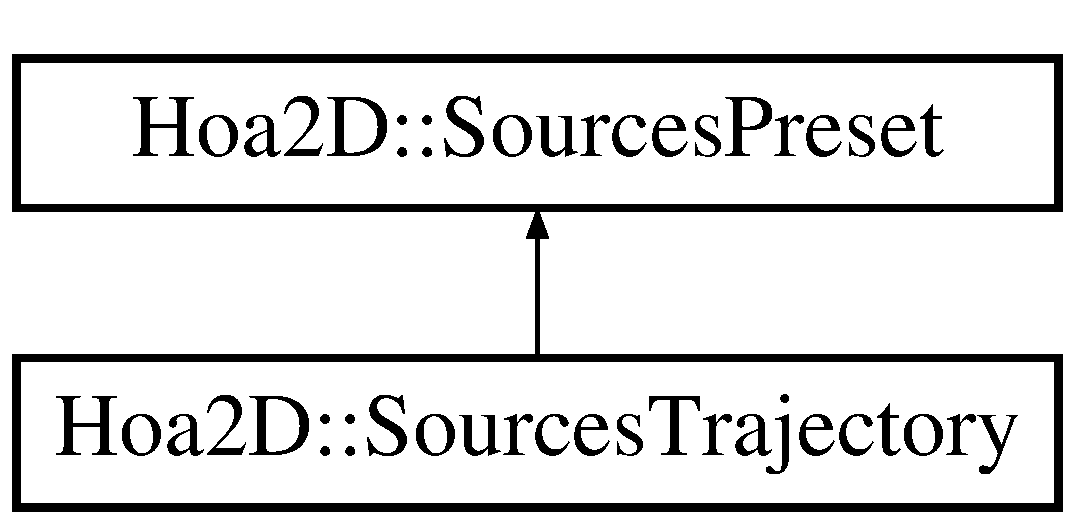
\includegraphics[height=2.000000cm]{class_hoa2_d_1_1_sources_preset}
\end{center}
\end{figure}
\subsection*{Public Member Functions}
\begin{DoxyCompactItemize}
\item 
\hyperlink{class_hoa2_d_1_1_sources_preset_aafde5df31f71153b72204466d443fc60}{Sources\-Preset} ()
\begin{DoxyCompactList}\small\item\em The source preset constructor. \end{DoxyCompactList}\item 
\hypertarget{class_hoa2_d_1_1_sources_preset_a2cc55290d42ea26d556c76845ac289c6}{\hyperlink{class_hoa2_d_1_1_sources_preset_a2cc55290d42ea26d556c76845ac289c6}{$\sim$\-Sources\-Preset} ()}\label{class_hoa2_d_1_1_sources_preset_a2cc55290d42ea26d556c76845ac289c6}

\begin{DoxyCompactList}\small\item\em The source preset destructor free the memory. \end{DoxyCompactList}\item 
void \hyperlink{class_hoa2_d_1_1_sources_preset_aa5a9db953bfffc3af48c7f052ff7d114}{store\-Source\-Manager\-At\-Slot} (\hyperlink{class_hoa2_d_1_1_sources_manager}{Sources\-Manager} $\ast$sources\-Manager, long index)
\begin{DoxyCompactList}\small\item\em Store a \hyperlink{class_hoa2_d_1_1_sources_manager}{Sources\-Manager} object at a particular slot index. \end{DoxyCompactList}\item 
void \hyperlink{class_hoa2_d_1_1_sources_preset_aafece46a576cec4a8c24ff04393a6879}{store\-Source\-Manager\-At\-First\-Empty\-Slot} (\hyperlink{class_hoa2_d_1_1_sources_manager}{Sources\-Manager} $\ast$sources\-Manager)
\begin{DoxyCompactList}\small\item\em Store a \hyperlink{class_hoa2_d_1_1_sources_manager}{Sources\-Manager} object at the first empty slot. \end{DoxyCompactList}\item 
void \hyperlink{class_hoa2_d_1_1_sources_preset_ade9e266d04987e3336aa30ee06026a5c}{store\-Source\-Manager\-At\-Last\-Used\-Slot} (\hyperlink{class_hoa2_d_1_1_sources_manager}{Sources\-Manager} $\ast$sources\-Manager)
\begin{DoxyCompactList}\small\item\em Store a \hyperlink{class_hoa2_d_1_1_sources_manager}{Sources\-Manager} object at the last used slot. \end{DoxyCompactList}\item 
void \hyperlink{class_hoa2_d_1_1_sources_preset_a67415a5175c688503b4f9621f558a4b6}{store\-Source\-Manager\-At\-New\-End\-Slot} (\hyperlink{class_hoa2_d_1_1_sources_manager}{Sources\-Manager} $\ast$sources\-Manager)
\begin{DoxyCompactList}\small\item\em Store a \hyperlink{class_hoa2_d_1_1_sources_manager}{Sources\-Manager} object in a new slot. \end{DoxyCompactList}\item 
void \hyperlink{class_hoa2_d_1_1_sources_preset_a2ebb6dc23c37ef95c4612ee093d5df2e}{store\-Source\-Manager\-At\-Next\-Slot} (\hyperlink{class_hoa2_d_1_1_sources_manager}{Sources\-Manager} $\ast$sources\-Manager)
\begin{DoxyCompactList}\small\item\em Store a \hyperlink{class_hoa2_d_1_1_sources_manager}{Sources\-Manager} object at the next slot. \end{DoxyCompactList}\item 
void \hyperlink{class_hoa2_d_1_1_sources_preset_a1b222c53d1ce33556595c7b16477cc8c}{insert\-Slot} (\hyperlink{class_hoa2_d_1_1_sources_manager}{Sources\-Manager} $\ast$sources\-Manager, long index)
\begin{DoxyCompactList}\small\item\em Store a \hyperlink{class_hoa2_d_1_1_sources_manager}{Sources\-Manager} object by inserting it at a particular slot index. \end{DoxyCompactList}\item 
void \hyperlink{class_hoa2_d_1_1_sources_preset_aaab4fce35fcf185b08abd056c61ef930}{remove\-Slot} (long index)
\begin{DoxyCompactList}\small\item\em Delete the content of a slot. \end{DoxyCompactList}\item 
void \hyperlink{class_hoa2_d_1_1_sources_preset_a2e3564af83143c51f826c4a0a4366ab9}{delete\-Slot} (long index)
\begin{DoxyCompactList}\small\item\em Delete the slot and its content. \end{DoxyCompactList}\item 
void \hyperlink{class_hoa2_d_1_1_sources_preset_a6fd54f266d7aee8e7b0dca9e1c5d4ab6}{copy\-Slot} (long source\-Index, long destination\-Index)
\begin{DoxyCompactList}\small\item\em Copy the content of a slot into another slot. \end{DoxyCompactList}\item 
\hypertarget{class_hoa2_d_1_1_sources_preset_ae23c21b6e292b25e154064523236ce17}{void \hyperlink{class_hoa2_d_1_1_sources_preset_ae23c21b6e292b25e154064523236ce17}{renumber} ()}\label{class_hoa2_d_1_1_sources_preset_ae23c21b6e292b25e154064523236ce17}

\begin{DoxyCompactList}\small\item\em Renumber all slots. \end{DoxyCompactList}\item 
\hypertarget{class_hoa2_d_1_1_sources_preset_a5a0c7de3777e9a3d4d1adb023ba02fff}{void \hyperlink{class_hoa2_d_1_1_sources_preset_a5a0c7de3777e9a3d4d1adb023ba02fff}{clear} ()}\label{class_hoa2_d_1_1_sources_preset_a5a0c7de3777e9a3d4d1adb023ba02fff}

\begin{DoxyCompactList}\small\item\em Clear all slots. \end{DoxyCompactList}\item 
void \hyperlink{class_hoa2_d_1_1_sources_preset_add27861d6a85c0fc48d1bebcd85581d0}{store\-Source\-At\-Slot} (\hyperlink{class_hoa2_d_1_1_sources_manager}{Sources\-Manager} $\ast$sources\-Manager, long slot\-Index, long source\-Index)
\begin{DoxyCompactList}\small\item\em Store a source at a given slot index. \end{DoxyCompactList}\item 
void \hyperlink{class_hoa2_d_1_1_sources_preset_a21a0a63a4c668845f5c5a5d7c4738697}{store\-Source\-At\-Next\-Slot} (\hyperlink{class_hoa2_d_1_1_sources_manager}{Sources\-Manager} $\ast$sources\-Manager, long source\-Index)
\begin{DoxyCompactList}\small\item\em Store a source at the next slot. \end{DoxyCompactList}\item 
void \hyperlink{class_hoa2_d_1_1_sources_preset_a5c27b7ef613359eeac422f018d023147}{store\-Group\-At\-Slot} (\hyperlink{class_hoa2_d_1_1_sources_manager}{Sources\-Manager} $\ast$sources\-Manager, long slot\-Index, long group\-Index)
\begin{DoxyCompactList}\small\item\em Store a group of source at a given slot index. \end{DoxyCompactList}\item 
void \hyperlink{class_hoa2_d_1_1_sources_preset_a272fc71db53b8572932360352bd87b64}{store\-Group\-At\-Next\-Slot} (\hyperlink{class_hoa2_d_1_1_sources_manager}{Sources\-Manager} $\ast$sources\-Manager, long group\-Index)
\begin{DoxyCompactList}\small\item\em Store a group at the next slot. \end{DoxyCompactList}\item 
void \hyperlink{class_hoa2_d_1_1_sources_preset_aef5a6ad6bb221517235fbddf05de3e31}{recall\-Slot} (\hyperlink{class_hoa2_d_1_1_sources_manager}{Sources\-Manager} $\ast$sources\-Manager, long index)
\begin{DoxyCompactList}\small\item\em Recall a given slot. \end{DoxyCompactList}\item 
void \hyperlink{class_hoa2_d_1_1_sources_preset_a4a3e373550dd48727b9d16586e546ec8}{recall\-Fractional\-Slot} (\hyperlink{class_hoa2_d_1_1_sources_manager}{Sources\-Manager} $\ast$sources\-Manager, long source\-Index, long destination\-Index, double fractionnal\-Index)
\begin{DoxyCompactList}\small\item\em Recall a given slot at a fractionnal index between two slot index. \end{DoxyCompactList}\item 
long \hyperlink{class_hoa2_d_1_1_sources_preset_a81b9d06eac962204b2b1c7ee93f03d46}{recall\-Fractional\-Slot} (\hyperlink{class_hoa2_d_1_1_sources_manager}{Sources\-Manager} $\ast$sources\-Manager, double fractionnal\-Index)
\begin{DoxyCompactList}\small\item\em Recall a given slot at a fractionnal index between two consecutive slot. \end{DoxyCompactList}\item 
\hypertarget{class_hoa2_d_1_1_sources_preset_a47d31bbb24565d050c44acf109fb959c}{long \hyperlink{class_hoa2_d_1_1_sources_preset_a47d31bbb24565d050c44acf109fb959c}{get\-Maximum\-Index\-Of\-Slot} ()}\label{class_hoa2_d_1_1_sources_preset_a47d31bbb24565d050c44acf109fb959c}

\begin{DoxyCompactList}\small\item\em Get The maximum index of slots. \end{DoxyCompactList}\item 
long \hyperlink{class_hoa2_d_1_1_sources_preset_a41fa4317089deb163f149e84248e2d0e}{get\-Slot\-Existence} (long index)
\begin{DoxyCompactList}\small\item\em Get the existence state of a given slot. \end{DoxyCompactList}\end{DoxyCompactItemize}


\subsection{Detailed Description}
The sources preset. 

The \hyperlink{class_hoa2_d_1_1_sources_preset}{Sources\-Preset} should be used to manage sources and group presets 

Definition at line 18 of file Sources\-Preset.\-h.



\subsection{Constructor \& Destructor Documentation}
\hypertarget{class_hoa2_d_1_1_sources_preset_aafde5df31f71153b72204466d443fc60}{\index{Hoa2\-D\-::\-Sources\-Preset@{Hoa2\-D\-::\-Sources\-Preset}!Sources\-Preset@{Sources\-Preset}}
\index{Sources\-Preset@{Sources\-Preset}!Hoa2D::SourcesPreset@{Hoa2\-D\-::\-Sources\-Preset}}
\subsubsection[{Sources\-Preset}]{\setlength{\rightskip}{0pt plus 5cm}Hoa2\-D\-::\-Sources\-Preset\-::\-Sources\-Preset (
\begin{DoxyParamCaption}
{}
\end{DoxyParamCaption}
)}}\label{class_hoa2_d_1_1_sources_preset_aafde5df31f71153b72204466d443fc60}


The source preset constructor. 

The source preset constructor allocates and initialize the member values. 

Definition at line 11 of file Sources\-Preset.\-cpp.



\subsection{Member Function Documentation}
\hypertarget{class_hoa2_d_1_1_sources_preset_a6fd54f266d7aee8e7b0dca9e1c5d4ab6}{\index{Hoa2\-D\-::\-Sources\-Preset@{Hoa2\-D\-::\-Sources\-Preset}!copy\-Slot@{copy\-Slot}}
\index{copy\-Slot@{copy\-Slot}!Hoa2D::SourcesPreset@{Hoa2\-D\-::\-Sources\-Preset}}
\subsubsection[{copy\-Slot}]{\setlength{\rightskip}{0pt plus 5cm}void Hoa2\-D\-::\-Sources\-Preset\-::copy\-Slot (
\begin{DoxyParamCaption}
\item[{long}]{source\-Index, }
\item[{long}]{destination\-Index}
\end{DoxyParamCaption}
)}}\label{class_hoa2_d_1_1_sources_preset_a6fd54f266d7aee8e7b0dca9e1c5d4ab6}


Copy the content of a slot into another slot. 


\begin{DoxyParams}{Parameters}
{\em source\-Index} & The index of the slot to copy. \\
\hline
{\em destination\-Index} & The index of the slot to copy in. \\
\hline
\end{DoxyParams}


Definition at line 297 of file Sources\-Preset.\-cpp.

\hypertarget{class_hoa2_d_1_1_sources_preset_a2e3564af83143c51f826c4a0a4366ab9}{\index{Hoa2\-D\-::\-Sources\-Preset@{Hoa2\-D\-::\-Sources\-Preset}!delete\-Slot@{delete\-Slot}}
\index{delete\-Slot@{delete\-Slot}!Hoa2D::SourcesPreset@{Hoa2\-D\-::\-Sources\-Preset}}
\subsubsection[{delete\-Slot}]{\setlength{\rightskip}{0pt plus 5cm}void Hoa2\-D\-::\-Sources\-Preset\-::delete\-Slot (
\begin{DoxyParamCaption}
\item[{long}]{index}
\end{DoxyParamCaption}
)}}\label{class_hoa2_d_1_1_sources_preset_a2e3564af83143c51f826c4a0a4366ab9}


Delete the slot and its content. 


\begin{DoxyParams}{Parameters}
{\em index} & The index of the slot. \\
\hline
\end{DoxyParams}


Definition at line 282 of file Sources\-Preset.\-cpp.

\hypertarget{class_hoa2_d_1_1_sources_preset_a41fa4317089deb163f149e84248e2d0e}{\index{Hoa2\-D\-::\-Sources\-Preset@{Hoa2\-D\-::\-Sources\-Preset}!get\-Slot\-Existence@{get\-Slot\-Existence}}
\index{get\-Slot\-Existence@{get\-Slot\-Existence}!Hoa2D::SourcesPreset@{Hoa2\-D\-::\-Sources\-Preset}}
\subsubsection[{get\-Slot\-Existence}]{\setlength{\rightskip}{0pt plus 5cm}long Hoa2\-D\-::\-Sources\-Preset\-::get\-Slot\-Existence (
\begin{DoxyParamCaption}
\item[{long}]{index}
\end{DoxyParamCaption}
)}}\label{class_hoa2_d_1_1_sources_preset_a41fa4317089deb163f149e84248e2d0e}


Get the existence state of a given slot. 


\begin{DoxyParams}{Parameters}
{\em index} & The index of the slot. \\
\hline
\end{DoxyParams}


Definition at line 440 of file Sources\-Preset.\-cpp.

\hypertarget{class_hoa2_d_1_1_sources_preset_a1b222c53d1ce33556595c7b16477cc8c}{\index{Hoa2\-D\-::\-Sources\-Preset@{Hoa2\-D\-::\-Sources\-Preset}!insert\-Slot@{insert\-Slot}}
\index{insert\-Slot@{insert\-Slot}!Hoa2D::SourcesPreset@{Hoa2\-D\-::\-Sources\-Preset}}
\subsubsection[{insert\-Slot}]{\setlength{\rightskip}{0pt plus 5cm}void Hoa2\-D\-::\-Sources\-Preset\-::insert\-Slot (
\begin{DoxyParamCaption}
\item[{{\bf Sources\-Manager} $\ast$}]{sources\-Manager, }
\item[{long}]{index}
\end{DoxyParamCaption}
)}}\label{class_hoa2_d_1_1_sources_preset_a1b222c53d1ce33556595c7b16477cc8c}


Store a \hyperlink{class_hoa2_d_1_1_sources_manager}{Sources\-Manager} object by inserting it at a particular slot index. 


\begin{DoxyParams}{Parameters}
{\em sources\-Manager} & A \hyperlink{class_hoa2_d_1_1_sources_manager}{Sources\-Manager} object pointer. \\
\hline
{\em index} & The index of the slot. \\
\hline
\end{DoxyParams}


Definition at line 253 of file Sources\-Preset.\-cpp.

\hypertarget{class_hoa2_d_1_1_sources_preset_a4a3e373550dd48727b9d16586e546ec8}{\index{Hoa2\-D\-::\-Sources\-Preset@{Hoa2\-D\-::\-Sources\-Preset}!recall\-Fractional\-Slot@{recall\-Fractional\-Slot}}
\index{recall\-Fractional\-Slot@{recall\-Fractional\-Slot}!Hoa2D::SourcesPreset@{Hoa2\-D\-::\-Sources\-Preset}}
\subsubsection[{recall\-Fractional\-Slot}]{\setlength{\rightskip}{0pt plus 5cm}void Hoa2\-D\-::\-Sources\-Preset\-::recall\-Fractional\-Slot (
\begin{DoxyParamCaption}
\item[{{\bf Sources\-Manager} $\ast$}]{sources\-Manager, }
\item[{long}]{source\-Index, }
\item[{long}]{destination\-Index, }
\item[{double}]{fractionnal\-Index}
\end{DoxyParamCaption}
)}}\label{class_hoa2_d_1_1_sources_preset_a4a3e373550dd48727b9d16586e546ec8}


Recall a given slot at a fractionnal index between two slot index. 

Interpolate between two \hyperlink{class_hoa2_d_1_1_sources_manager}{Sources\-Manager}'s states. 
\begin{DoxyParams}{Parameters}
{\em sources\-Manager} & A \hyperlink{class_hoa2_d_1_1_sources_manager}{Sources\-Manager} object pointer. \\
\hline
{\em source\-Index} & Index of the first slot. \\
\hline
{\em destination\-Index} & Index of the second slot. \\
\hline
{\em fractionnal\-Index} & The fractionnal index (between 0 and 1). \\
\hline
\end{DoxyParams}
\begin{DoxySeeAlso}{See Also}
\hyperlink{class_hoa2_d_1_1_sources_preset_a4a3e373550dd48727b9d16586e546ec8}{recall\-Fractional\-Slot} 
\end{DoxySeeAlso}


Definition at line 342 of file Sources\-Preset.\-cpp.

\hypertarget{class_hoa2_d_1_1_sources_preset_a81b9d06eac962204b2b1c7ee93f03d46}{\index{Hoa2\-D\-::\-Sources\-Preset@{Hoa2\-D\-::\-Sources\-Preset}!recall\-Fractional\-Slot@{recall\-Fractional\-Slot}}
\index{recall\-Fractional\-Slot@{recall\-Fractional\-Slot}!Hoa2D::SourcesPreset@{Hoa2\-D\-::\-Sources\-Preset}}
\subsubsection[{recall\-Fractional\-Slot}]{\setlength{\rightskip}{0pt plus 5cm}long Hoa2\-D\-::\-Sources\-Preset\-::recall\-Fractional\-Slot (
\begin{DoxyParamCaption}
\item[{{\bf Sources\-Manager} $\ast$}]{sources\-Manager, }
\item[{double}]{fractionnal\-Index}
\end{DoxyParamCaption}
)}}\label{class_hoa2_d_1_1_sources_preset_a81b9d06eac962204b2b1c7ee93f03d46}


Recall a given slot at a fractionnal index between two consecutive slot. 

Interpolate between two \hyperlink{class_hoa2_d_1_1_sources_manager}{Sources\-Manager}'s states. 
\begin{DoxyParams}{Parameters}
{\em sources\-Manager} & A \hyperlink{class_hoa2_d_1_1_sources_manager}{Sources\-Manager} object pointer. \\
\hline
{\em fractionnal\-Index} & The fractionnal index. (ex. 2.\-3 will interpolate between the slot 2 and slot 3) \\
\hline
\end{DoxyParams}
\begin{DoxySeeAlso}{See Also}
\hyperlink{class_hoa2_d_1_1_sources_preset_a4a3e373550dd48727b9d16586e546ec8}{recall\-Fractional\-Slot} 
\end{DoxySeeAlso}


Definition at line 354 of file Sources\-Preset.\-cpp.

\hypertarget{class_hoa2_d_1_1_sources_preset_aef5a6ad6bb221517235fbddf05de3e31}{\index{Hoa2\-D\-::\-Sources\-Preset@{Hoa2\-D\-::\-Sources\-Preset}!recall\-Slot@{recall\-Slot}}
\index{recall\-Slot@{recall\-Slot}!Hoa2D::SourcesPreset@{Hoa2\-D\-::\-Sources\-Preset}}
\subsubsection[{recall\-Slot}]{\setlength{\rightskip}{0pt plus 5cm}void Hoa2\-D\-::\-Sources\-Preset\-::recall\-Slot (
\begin{DoxyParamCaption}
\item[{{\bf Sources\-Manager} $\ast$}]{sources\-Manager, }
\item[{long}]{index}
\end{DoxyParamCaption}
)}}\label{class_hoa2_d_1_1_sources_preset_aef5a6ad6bb221517235fbddf05de3e31}


Recall a given slot. 

Recall \hyperlink{class_hoa2_d_1_1_sources_manager}{Sources\-Manager} state directly 
\begin{DoxyParams}{Parameters}
{\em sources\-Manager} & A \hyperlink{class_hoa2_d_1_1_sources_manager}{Sources\-Manager} object pointer. \\
\hline
{\em index} & The index of the slot. \\
\hline
\end{DoxyParams}
\begin{DoxySeeAlso}{See Also}
\hyperlink{class_hoa2_d_1_1_sources_preset_a4a3e373550dd48727b9d16586e546ec8}{recall\-Fractional\-Slot} 
\end{DoxySeeAlso}


Definition at line 333 of file Sources\-Preset.\-cpp.

\hypertarget{class_hoa2_d_1_1_sources_preset_aaab4fce35fcf185b08abd056c61ef930}{\index{Hoa2\-D\-::\-Sources\-Preset@{Hoa2\-D\-::\-Sources\-Preset}!remove\-Slot@{remove\-Slot}}
\index{remove\-Slot@{remove\-Slot}!Hoa2D::SourcesPreset@{Hoa2\-D\-::\-Sources\-Preset}}
\subsubsection[{remove\-Slot}]{\setlength{\rightskip}{0pt plus 5cm}void Hoa2\-D\-::\-Sources\-Preset\-::remove\-Slot (
\begin{DoxyParamCaption}
\item[{long}]{index}
\end{DoxyParamCaption}
)}}\label{class_hoa2_d_1_1_sources_preset_aaab4fce35fcf185b08abd056c61ef930}


Delete the content of a slot. 


\begin{DoxyParams}{Parameters}
{\em index} & The index of the slot. \\
\hline
\end{DoxyParams}


Definition at line 274 of file Sources\-Preset.\-cpp.

\hypertarget{class_hoa2_d_1_1_sources_preset_a272fc71db53b8572932360352bd87b64}{\index{Hoa2\-D\-::\-Sources\-Preset@{Hoa2\-D\-::\-Sources\-Preset}!store\-Group\-At\-Next\-Slot@{store\-Group\-At\-Next\-Slot}}
\index{store\-Group\-At\-Next\-Slot@{store\-Group\-At\-Next\-Slot}!Hoa2D::SourcesPreset@{Hoa2\-D\-::\-Sources\-Preset}}
\subsubsection[{store\-Group\-At\-Next\-Slot}]{\setlength{\rightskip}{0pt plus 5cm}void Hoa2\-D\-::\-Sources\-Preset\-::store\-Group\-At\-Next\-Slot (
\begin{DoxyParamCaption}
\item[{{\bf Sources\-Manager} $\ast$}]{sources\-Manager, }
\item[{long}]{group\-Index}
\end{DoxyParamCaption}
)}}\label{class_hoa2_d_1_1_sources_preset_a272fc71db53b8572932360352bd87b64}


Store a group at the next slot. 


\begin{DoxyParams}{Parameters}
{\em sources\-Manager} & A \hyperlink{class_hoa2_d_1_1_sources_manager}{Sources\-Manager} object pointer. \\
\hline
{\em slot\-Index} & The index of the slot. \\
\hline
{\em group\-Index} & The index of the group to store. \\
\hline
\end{DoxyParams}


Definition at line 247 of file Sources\-Preset.\-cpp.

\hypertarget{class_hoa2_d_1_1_sources_preset_a5c27b7ef613359eeac422f018d023147}{\index{Hoa2\-D\-::\-Sources\-Preset@{Hoa2\-D\-::\-Sources\-Preset}!store\-Group\-At\-Slot@{store\-Group\-At\-Slot}}
\index{store\-Group\-At\-Slot@{store\-Group\-At\-Slot}!Hoa2D::SourcesPreset@{Hoa2\-D\-::\-Sources\-Preset}}
\subsubsection[{store\-Group\-At\-Slot}]{\setlength{\rightskip}{0pt plus 5cm}void Hoa2\-D\-::\-Sources\-Preset\-::store\-Group\-At\-Slot (
\begin{DoxyParamCaption}
\item[{{\bf Sources\-Manager} $\ast$}]{sources\-Manager, }
\item[{long}]{slot\-Index, }
\item[{long}]{group\-Index}
\end{DoxyParamCaption}
)}}\label{class_hoa2_d_1_1_sources_preset_a5c27b7ef613359eeac422f018d023147}


Store a group of source at a given slot index. 


\begin{DoxyParams}{Parameters}
{\em sources\-Manager} & A \hyperlink{class_hoa2_d_1_1_sources_manager}{Sources\-Manager} object pointer. \\
\hline
{\em slot\-Index} & The index of the slot. \\
\hline
{\em group\-Index} & The index of the group to store. \\
\hline
\end{DoxyParams}


Definition at line 231 of file Sources\-Preset.\-cpp.

\hypertarget{class_hoa2_d_1_1_sources_preset_a21a0a63a4c668845f5c5a5d7c4738697}{\index{Hoa2\-D\-::\-Sources\-Preset@{Hoa2\-D\-::\-Sources\-Preset}!store\-Source\-At\-Next\-Slot@{store\-Source\-At\-Next\-Slot}}
\index{store\-Source\-At\-Next\-Slot@{store\-Source\-At\-Next\-Slot}!Hoa2D::SourcesPreset@{Hoa2\-D\-::\-Sources\-Preset}}
\subsubsection[{store\-Source\-At\-Next\-Slot}]{\setlength{\rightskip}{0pt plus 5cm}void Hoa2\-D\-::\-Sources\-Preset\-::store\-Source\-At\-Next\-Slot (
\begin{DoxyParamCaption}
\item[{{\bf Sources\-Manager} $\ast$}]{sources\-Manager, }
\item[{long}]{source\-Index}
\end{DoxyParamCaption}
)}}\label{class_hoa2_d_1_1_sources_preset_a21a0a63a4c668845f5c5a5d7c4738697}


Store a source at the next slot. 


\begin{DoxyParams}{Parameters}
{\em sources\-Manager} & A \hyperlink{class_hoa2_d_1_1_sources_manager}{Sources\-Manager} object pointer. \\
\hline
{\em slot\-Index} & The index of the slot. \\
\hline
{\em source\-Index} & The index of the source to store. \\
\hline
\end{DoxyParams}


Definition at line 226 of file Sources\-Preset.\-cpp.

\hypertarget{class_hoa2_d_1_1_sources_preset_add27861d6a85c0fc48d1bebcd85581d0}{\index{Hoa2\-D\-::\-Sources\-Preset@{Hoa2\-D\-::\-Sources\-Preset}!store\-Source\-At\-Slot@{store\-Source\-At\-Slot}}
\index{store\-Source\-At\-Slot@{store\-Source\-At\-Slot}!Hoa2D::SourcesPreset@{Hoa2\-D\-::\-Sources\-Preset}}
\subsubsection[{store\-Source\-At\-Slot}]{\setlength{\rightskip}{0pt plus 5cm}void Hoa2\-D\-::\-Sources\-Preset\-::store\-Source\-At\-Slot (
\begin{DoxyParamCaption}
\item[{{\bf Sources\-Manager} $\ast$}]{sources\-Manager, }
\item[{long}]{slot\-Index, }
\item[{long}]{source\-Index}
\end{DoxyParamCaption}
)}}\label{class_hoa2_d_1_1_sources_preset_add27861d6a85c0fc48d1bebcd85581d0}


Store a source at a given slot index. 


\begin{DoxyParams}{Parameters}
{\em sources\-Manager} & A \hyperlink{class_hoa2_d_1_1_sources_manager}{Sources\-Manager} object pointer. \\
\hline
{\em slot\-Index} & The index of the slot. \\
\hline
{\em source\-Index} & The index of the source to store. \\
\hline
\end{DoxyParams}


Definition at line 210 of file Sources\-Preset.\-cpp.

\hypertarget{class_hoa2_d_1_1_sources_preset_aafece46a576cec4a8c24ff04393a6879}{\index{Hoa2\-D\-::\-Sources\-Preset@{Hoa2\-D\-::\-Sources\-Preset}!store\-Source\-Manager\-At\-First\-Empty\-Slot@{store\-Source\-Manager\-At\-First\-Empty\-Slot}}
\index{store\-Source\-Manager\-At\-First\-Empty\-Slot@{store\-Source\-Manager\-At\-First\-Empty\-Slot}!Hoa2D::SourcesPreset@{Hoa2\-D\-::\-Sources\-Preset}}
\subsubsection[{store\-Source\-Manager\-At\-First\-Empty\-Slot}]{\setlength{\rightskip}{0pt plus 5cm}void Hoa2\-D\-::\-Sources\-Preset\-::store\-Source\-Manager\-At\-First\-Empty\-Slot (
\begin{DoxyParamCaption}
\item[{{\bf Sources\-Manager} $\ast$}]{sources\-Manager}
\end{DoxyParamCaption}
)}}\label{class_hoa2_d_1_1_sources_preset_aafece46a576cec4a8c24ff04393a6879}


Store a \hyperlink{class_hoa2_d_1_1_sources_manager}{Sources\-Manager} object at the first empty slot. 


\begin{DoxyParams}{Parameters}
{\em sources\-Manager} & A \hyperlink{class_hoa2_d_1_1_sources_manager}{Sources\-Manager} object pointer. \\
\hline
\end{DoxyParams}


Definition at line 181 of file Sources\-Preset.\-cpp.

\hypertarget{class_hoa2_d_1_1_sources_preset_ade9e266d04987e3336aa30ee06026a5c}{\index{Hoa2\-D\-::\-Sources\-Preset@{Hoa2\-D\-::\-Sources\-Preset}!store\-Source\-Manager\-At\-Last\-Used\-Slot@{store\-Source\-Manager\-At\-Last\-Used\-Slot}}
\index{store\-Source\-Manager\-At\-Last\-Used\-Slot@{store\-Source\-Manager\-At\-Last\-Used\-Slot}!Hoa2D::SourcesPreset@{Hoa2\-D\-::\-Sources\-Preset}}
\subsubsection[{store\-Source\-Manager\-At\-Last\-Used\-Slot}]{\setlength{\rightskip}{0pt plus 5cm}void Hoa2\-D\-::\-Sources\-Preset\-::store\-Source\-Manager\-At\-Last\-Used\-Slot (
\begin{DoxyParamCaption}
\item[{{\bf Sources\-Manager} $\ast$}]{sources\-Manager}
\end{DoxyParamCaption}
)}}\label{class_hoa2_d_1_1_sources_preset_ade9e266d04987e3336aa30ee06026a5c}


Store a \hyperlink{class_hoa2_d_1_1_sources_manager}{Sources\-Manager} object at the last used slot. 


\begin{DoxyParams}{Parameters}
{\em sources\-Manager} & A \hyperlink{class_hoa2_d_1_1_sources_manager}{Sources\-Manager} object pointer. \\
\hline
\end{DoxyParams}


Definition at line 195 of file Sources\-Preset.\-cpp.

\hypertarget{class_hoa2_d_1_1_sources_preset_a67415a5175c688503b4f9621f558a4b6}{\index{Hoa2\-D\-::\-Sources\-Preset@{Hoa2\-D\-::\-Sources\-Preset}!store\-Source\-Manager\-At\-New\-End\-Slot@{store\-Source\-Manager\-At\-New\-End\-Slot}}
\index{store\-Source\-Manager\-At\-New\-End\-Slot@{store\-Source\-Manager\-At\-New\-End\-Slot}!Hoa2D::SourcesPreset@{Hoa2\-D\-::\-Sources\-Preset}}
\subsubsection[{store\-Source\-Manager\-At\-New\-End\-Slot}]{\setlength{\rightskip}{0pt plus 5cm}void Hoa2\-D\-::\-Sources\-Preset\-::store\-Source\-Manager\-At\-New\-End\-Slot (
\begin{DoxyParamCaption}
\item[{{\bf Sources\-Manager} $\ast$}]{sources\-Manager}
\end{DoxyParamCaption}
)}}\label{class_hoa2_d_1_1_sources_preset_a67415a5175c688503b4f9621f558a4b6}


Store a \hyperlink{class_hoa2_d_1_1_sources_manager}{Sources\-Manager} object in a new slot. 


\begin{DoxyParams}{Parameters}
{\em sources\-Manager} & A \hyperlink{class_hoa2_d_1_1_sources_manager}{Sources\-Manager} object pointer. \\
\hline
\end{DoxyParams}


Definition at line 205 of file Sources\-Preset.\-cpp.

\hypertarget{class_hoa2_d_1_1_sources_preset_a2ebb6dc23c37ef95c4612ee093d5df2e}{\index{Hoa2\-D\-::\-Sources\-Preset@{Hoa2\-D\-::\-Sources\-Preset}!store\-Source\-Manager\-At\-Next\-Slot@{store\-Source\-Manager\-At\-Next\-Slot}}
\index{store\-Source\-Manager\-At\-Next\-Slot@{store\-Source\-Manager\-At\-Next\-Slot}!Hoa2D::SourcesPreset@{Hoa2\-D\-::\-Sources\-Preset}}
\subsubsection[{store\-Source\-Manager\-At\-Next\-Slot}]{\setlength{\rightskip}{0pt plus 5cm}void Hoa2\-D\-::\-Sources\-Preset\-::store\-Source\-Manager\-At\-Next\-Slot (
\begin{DoxyParamCaption}
\item[{{\bf Sources\-Manager} $\ast$}]{sources\-Manager}
\end{DoxyParamCaption}
)}}\label{class_hoa2_d_1_1_sources_preset_a2ebb6dc23c37ef95c4612ee093d5df2e}


Store a \hyperlink{class_hoa2_d_1_1_sources_manager}{Sources\-Manager} object at the next slot. 


\begin{DoxyParams}{Parameters}
{\em sources\-Manager} & A \hyperlink{class_hoa2_d_1_1_sources_manager}{Sources\-Manager} object pointer. \\
\hline
\end{DoxyParams}


Definition at line 200 of file Sources\-Preset.\-cpp.

\hypertarget{class_hoa2_d_1_1_sources_preset_aa5a9db953bfffc3af48c7f052ff7d114}{\index{Hoa2\-D\-::\-Sources\-Preset@{Hoa2\-D\-::\-Sources\-Preset}!store\-Source\-Manager\-At\-Slot@{store\-Source\-Manager\-At\-Slot}}
\index{store\-Source\-Manager\-At\-Slot@{store\-Source\-Manager\-At\-Slot}!Hoa2D::SourcesPreset@{Hoa2\-D\-::\-Sources\-Preset}}
\subsubsection[{store\-Source\-Manager\-At\-Slot}]{\setlength{\rightskip}{0pt plus 5cm}void Hoa2\-D\-::\-Sources\-Preset\-::store\-Source\-Manager\-At\-Slot (
\begin{DoxyParamCaption}
\item[{{\bf Sources\-Manager} $\ast$}]{sources\-Manager, }
\item[{long}]{index}
\end{DoxyParamCaption}
)}}\label{class_hoa2_d_1_1_sources_preset_aa5a9db953bfffc3af48c7f052ff7d114}


Store a \hyperlink{class_hoa2_d_1_1_sources_manager}{Sources\-Manager} object at a particular slot index. 


\begin{DoxyParams}{Parameters}
{\em sources\-Manager} & A \hyperlink{class_hoa2_d_1_1_sources_manager}{Sources\-Manager} object pointer. \\
\hline
{\em index} & The index of the slot. \\
\hline
\end{DoxyParams}


Definition at line 165 of file Sources\-Preset.\-cpp.


\hypertarget{class_hoa2_d_1_1_sources_trajectory}{\section{Hoa2\-D\-:\-:Sources\-Trajectory Class Reference}
\label{class_hoa2_d_1_1_sources_trajectory}\index{Hoa2\-D\-::\-Sources\-Trajectory@{Hoa2\-D\-::\-Sources\-Trajectory}}
}
Inheritance diagram for Hoa2\-D\-:\-:Sources\-Trajectory\-:\begin{figure}[H]
\begin{center}
\leavevmode
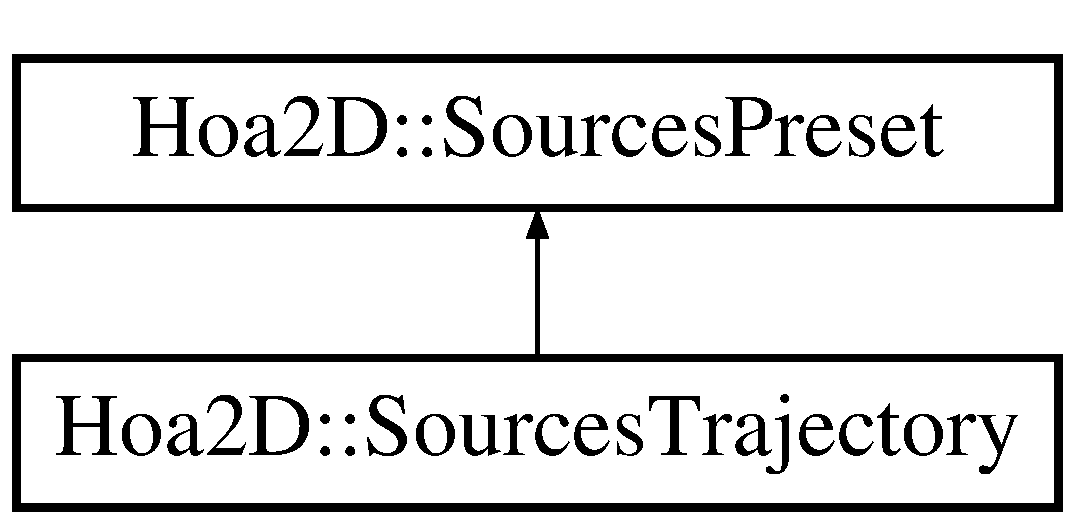
\includegraphics[height=2.000000cm]{class_hoa2_d_1_1_sources_trajectory}
\end{center}
\end{figure}


\subsection{Detailed Description}


Definition at line 14 of file Sources\-Trajectory.\-h.



The documentation for this class was generated from the following files\-:\begin{DoxyCompactItemize}
\item 
/\-Users/\-Pierre/\-Source\-Tree/\-Hoa\-Library/\-Sources/\-Hoa2\-D/Sources\-Trajectory.\-h\item 
/\-Users/\-Pierre/\-Source\-Tree/\-Hoa\-Library/\-Sources/\-Hoa2\-D/Sources\-Trajectory.\-cpp\end{DoxyCompactItemize}

\hypertarget{class_tools}{\section{Tools Class Reference}
\label{class_tools}\index{Tools@{Tools}}
}


\subsection{Detailed Description}


Definition at line 68 of file Cicm\-Tools.\-h.



The documentation for this class was generated from the following file\-:\begin{DoxyCompactItemize}
\item 
/\-Users/\-Pierre/\-Source\-Tree/\-Hoa\-Library/\-Sources/\-Cicm\-Library/Cicm\-Tools.\-h\end{DoxyCompactItemize}

\hypertarget{class_hoa2_d_1_1_vector}{\section{Hoa2\-D\-:\-:Vector Class Reference}
\label{class_hoa2_d_1_1_vector}\index{Hoa2\-D\-::\-Vector@{Hoa2\-D\-::\-Vector}}
}


The ambisonic vector.  




{\ttfamily \#include $<$Vector.\-h$>$}

Inheritance diagram for Hoa2\-D\-:\-:Vector\-:\begin{figure}[H]
\begin{center}
\leavevmode
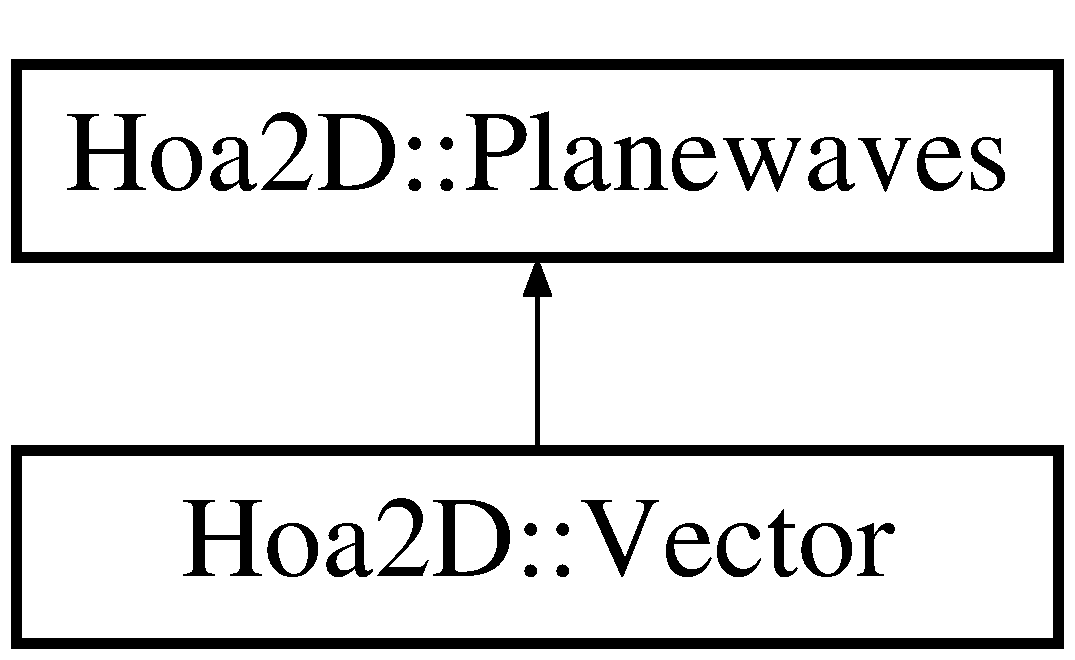
\includegraphics[height=2.000000cm]{class_hoa2_d_1_1_vector}
\end{center}
\end{figure}
\subsection*{Public Member Functions}
\begin{DoxyCompactItemize}
\item 
\hyperlink{class_hoa2_d_1_1_vector_aee9bdb6355b741ca4ae90286745de397}{Vector} (unsigned int number\-Of\-Channels)
\begin{DoxyCompactList}\small\item\em The vector constructor. \end{DoxyCompactList}\item 
\hyperlink{class_hoa2_d_1_1_vector_aa260b1636ddc02ac37279f1b3c6160da}{$\sim$\-Vector} ()
\begin{DoxyCompactList}\small\item\em The optimization destructor. \end{DoxyCompactList}\item 
void \hyperlink{class_hoa2_d_1_1_vector_a4bc03e92cd2bd7a2ffb4f8c3358631f6}{set\-Channel\-Position} (unsigned int index, double azimuth)
\begin{DoxyCompactList}\small\item\em Set the azimtuh of a channel. \end{DoxyCompactList}\item 
void \hyperlink{class_hoa2_d_1_1_vector_aba460ca0df1e870dcb958771b9687d9b}{process} (const float $\ast$inputs, float $\ast$outputs)
\begin{DoxyCompactList}\small\item\em This method compute the energy and velocity vectors with single precision. \end{DoxyCompactList}\item 
void \hyperlink{class_hoa2_d_1_1_vector_a3715759c77efd66a05f19a0b62387700}{process} (const double $\ast$inputs, double $\ast$outputs)
\begin{DoxyCompactList}\small\item\em This method compute the energy and velocity vectors with double precision. \end{DoxyCompactList}\item 
void \hyperlink{class_hoa2_d_1_1_vector_a439e3c413c03c40abd0b3c836ccd92dc}{process\-Velocity} (const float $\ast$inputs, float $\ast$outputs)
\begin{DoxyCompactList}\small\item\em This method compute the velocity vector with single precision. \end{DoxyCompactList}\item 
void \hyperlink{class_hoa2_d_1_1_vector_ab7804e8ec5322fe018141015a8683bd4}{process\-Velocity} (const double $\ast$inputs, double $\ast$outputs)
\begin{DoxyCompactList}\small\item\em This method compute the velocity vector with double precision. \end{DoxyCompactList}\item 
void \hyperlink{class_hoa2_d_1_1_vector_aa24ad96a21db0f508282a8c94a848e1d}{process\-Energy} (const float $\ast$inputs, float $\ast$outputs)
\begin{DoxyCompactList}\small\item\em This method compute the energy vector with single precision. \end{DoxyCompactList}\item 
void \hyperlink{class_hoa2_d_1_1_vector_a6d91bf205b88b88acdc53177e833da59}{process\-Energy} (const double $\ast$inputs, double $\ast$outputs)
\begin{DoxyCompactList}\small\item\em This method compute the energy vector with double precision. \end{DoxyCompactList}\end{DoxyCompactItemize}
\subsection*{Additional Inherited Members}


\subsection{Detailed Description}
The ambisonic vector. 

The vector class compute the energy and the velocity vector of a soudfield for a set of loudspeakers. It is an useful tool to characterize the quality of the sound field resitution. For futher information \-: Michael A. Gerzon, General metatheorie of auditory localisation. Audio Engineering Society Preprint, 3306, 1992. This class retreive the cartesian coordinates of the vectors, the abscissa and the ordinate. 

Definition at line 17 of file Vector.\-h.



\subsection{Constructor \& Destructor Documentation}
\hypertarget{class_hoa2_d_1_1_vector_aee9bdb6355b741ca4ae90286745de397}{\index{Hoa2\-D\-::\-Vector@{Hoa2\-D\-::\-Vector}!Vector@{Vector}}
\index{Vector@{Vector}!Hoa2D::Vector@{Hoa2\-D\-::\-Vector}}
\subsubsection[{Vector}]{\setlength{\rightskip}{0pt plus 5cm}Hoa2\-D\-::\-Vector\-::\-Vector (
\begin{DoxyParamCaption}
\item[{unsigned int}]{number\-Of\-Channels}
\end{DoxyParamCaption}
)}}\label{class_hoa2_d_1_1_vector_aee9bdb6355b741ca4ae90286745de397}


The vector constructor. 

The optimization constructor allocates and initialize the member values to computes vectors. The number of channels must be at least 1.


\begin{DoxyParams}{Parameters}
{\em number\-Of\-Channels} & The number of loudspeakers. \\
\hline
\end{DoxyParams}


Definition at line 11 of file Vector.\-cpp.

\hypertarget{class_hoa2_d_1_1_vector_aa260b1636ddc02ac37279f1b3c6160da}{\index{Hoa2\-D\-::\-Vector@{Hoa2\-D\-::\-Vector}!$\sim$\-Vector@{$\sim$\-Vector}}
\index{$\sim$\-Vector@{$\sim$\-Vector}!Hoa2D::Vector@{Hoa2\-D\-::\-Vector}}
\subsubsection[{$\sim$\-Vector}]{\setlength{\rightskip}{0pt plus 5cm}Hoa2\-D\-::\-Vector\-::$\sim$\-Vector (
\begin{DoxyParamCaption}
{}
\end{DoxyParamCaption}
)}}\label{class_hoa2_d_1_1_vector_aa260b1636ddc02ac37279f1b3c6160da}


The optimization destructor. 

The optimization destructor free the memory. 

Definition at line 134 of file Vector.\-cpp.



\subsection{Member Function Documentation}
\hypertarget{class_hoa2_d_1_1_vector_aba460ca0df1e870dcb958771b9687d9b}{\index{Hoa2\-D\-::\-Vector@{Hoa2\-D\-::\-Vector}!process@{process}}
\index{process@{process}!Hoa2D::Vector@{Hoa2\-D\-::\-Vector}}
\subsubsection[{process}]{\setlength{\rightskip}{0pt plus 5cm}void Hoa2\-D\-::\-Vector\-::process (
\begin{DoxyParamCaption}
\item[{const float $\ast$}]{inputs, }
\item[{float $\ast$}]{outputs}
\end{DoxyParamCaption}
)}}\label{class_hoa2_d_1_1_vector_aba460ca0df1e870dcb958771b9687d9b}


This method compute the energy and velocity vectors with single precision. 

You should use this method for in-\/place or not-\/in-\/place processing and compute the vectors sample by sample. The inputs array and contains the channels samples and the minimum size must be the number of harmonics. The outputs array contains the vectors cartesian coordinates and the minimum size must be 4. The coordinates arrengement in the outputs array is velocity abscissa, velocity ordinate, energy abscissa, energy ordinate.


\begin{DoxyParams}{Parameters}
{\em inputs} & The inputs array. \\
\hline
{\em outputs} & The outputs array. \\
\hline
\end{DoxyParams}


Definition at line 122 of file Vector.\-cpp.

\hypertarget{class_hoa2_d_1_1_vector_a3715759c77efd66a05f19a0b62387700}{\index{Hoa2\-D\-::\-Vector@{Hoa2\-D\-::\-Vector}!process@{process}}
\index{process@{process}!Hoa2D::Vector@{Hoa2\-D\-::\-Vector}}
\subsubsection[{process}]{\setlength{\rightskip}{0pt plus 5cm}void Hoa2\-D\-::\-Vector\-::process (
\begin{DoxyParamCaption}
\item[{const double $\ast$}]{inputs, }
\item[{double $\ast$}]{outputs}
\end{DoxyParamCaption}
)}}\label{class_hoa2_d_1_1_vector_a3715759c77efd66a05f19a0b62387700}


This method compute the energy and velocity vectors with double precision. 

You should use this method for in-\/place or not-\/in-\/place processing and compute the vectors sample by sample. The inputs array and contains the channels samples and the minimum size must be the number of harmonics. The outputs array contains the vectors cartesian coordinates and the minimum size must be 4. The coordinates arrengement in the outputs array is velocity abscissa, velocity ordinate, energy abscissa, energy ordinate.


\begin{DoxyParams}{Parameters}
{\em inputs} & The inputs array. \\
\hline
{\em outputs} & The outputs array. \\
\hline
\end{DoxyParams}


Definition at line 128 of file Vector.\-cpp.

\hypertarget{class_hoa2_d_1_1_vector_aa24ad96a21db0f508282a8c94a848e1d}{\index{Hoa2\-D\-::\-Vector@{Hoa2\-D\-::\-Vector}!process\-Energy@{process\-Energy}}
\index{process\-Energy@{process\-Energy}!Hoa2D::Vector@{Hoa2\-D\-::\-Vector}}
\subsubsection[{process\-Energy}]{\setlength{\rightskip}{0pt plus 5cm}void Hoa2\-D\-::\-Vector\-::process\-Energy (
\begin{DoxyParamCaption}
\item[{const float $\ast$}]{inputs, }
\item[{float $\ast$}]{outputs}
\end{DoxyParamCaption}
)}}\label{class_hoa2_d_1_1_vector_aa24ad96a21db0f508282a8c94a848e1d}


This method compute the energy vector with single precision. 

\begin{DoxyVerb}You should use this method for in-place or not-in-place processing and compute the vectors sample by sample. The inputs array and contains the channels samples and the minimum size must be the number of harmonics. The outputs array contains the vectors cartesian coordinates and the minimum size must be 2. The coordinates arrengement in the outputs array is energy abscissa, energy ordinate.
\end{DoxyVerb}



\begin{DoxyParams}{Parameters}
{\em inputs} & The inputs array. \\
\hline
{\em outputs} & The outputs array. \\
\hline
\end{DoxyParams}


Definition at line 75 of file Vector.\-cpp.

\hypertarget{class_hoa2_d_1_1_vector_a6d91bf205b88b88acdc53177e833da59}{\index{Hoa2\-D\-::\-Vector@{Hoa2\-D\-::\-Vector}!process\-Energy@{process\-Energy}}
\index{process\-Energy@{process\-Energy}!Hoa2D::Vector@{Hoa2\-D\-::\-Vector}}
\subsubsection[{process\-Energy}]{\setlength{\rightskip}{0pt plus 5cm}void Hoa2\-D\-::\-Vector\-::process\-Energy (
\begin{DoxyParamCaption}
\item[{const double $\ast$}]{inputs, }
\item[{double $\ast$}]{outputs}
\end{DoxyParamCaption}
)}}\label{class_hoa2_d_1_1_vector_a6d91bf205b88b88acdc53177e833da59}


This method compute the energy vector with double precision. 

\begin{DoxyVerb}You should use this method for in-place or not-in-place processing and compute the vectors sample by sample. The inputs array and contains the channels samples and the minimum size must be the number of harmonics. The outputs array contains the vectors cartesian coordinates and the minimum size must be 2. The coordinates arrengement in the outputs array is energy abscissa, energy ordinate.
\end{DoxyVerb}



\begin{DoxyParams}{Parameters}
{\em inputs} & The inputs array. \\
\hline
{\em outputs} & The outputs array. \\
\hline
\end{DoxyParams}


Definition at line 98 of file Vector.\-cpp.

\hypertarget{class_hoa2_d_1_1_vector_a439e3c413c03c40abd0b3c836ccd92dc}{\index{Hoa2\-D\-::\-Vector@{Hoa2\-D\-::\-Vector}!process\-Velocity@{process\-Velocity}}
\index{process\-Velocity@{process\-Velocity}!Hoa2D::Vector@{Hoa2\-D\-::\-Vector}}
\subsubsection[{process\-Velocity}]{\setlength{\rightskip}{0pt plus 5cm}void Hoa2\-D\-::\-Vector\-::process\-Velocity (
\begin{DoxyParamCaption}
\item[{const float $\ast$}]{inputs, }
\item[{float $\ast$}]{outputs}
\end{DoxyParamCaption}
)}}\label{class_hoa2_d_1_1_vector_a439e3c413c03c40abd0b3c836ccd92dc}


This method compute the velocity vector with single precision. 

\begin{DoxyVerb}You should use this method for in-place or not-in-place processing and compute the vectors sample by sample. The inputs array and contains the channels samples and the minimum size must be the number of harmonics. The outputs array contains the vectors cartesian coordinates and the minimum size must be 2. The coordinates arrengement in the outputs array is velocity abscissa, velocity ordinate.
\end{DoxyVerb}



\begin{DoxyParams}{Parameters}
{\em inputs} & The inputs array. \\
\hline
{\em outputs} & The outputs array. \\
\hline
\end{DoxyParams}


Definition at line 37 of file Vector.\-cpp.

\hypertarget{class_hoa2_d_1_1_vector_ab7804e8ec5322fe018141015a8683bd4}{\index{Hoa2\-D\-::\-Vector@{Hoa2\-D\-::\-Vector}!process\-Velocity@{process\-Velocity}}
\index{process\-Velocity@{process\-Velocity}!Hoa2D::Vector@{Hoa2\-D\-::\-Vector}}
\subsubsection[{process\-Velocity}]{\setlength{\rightskip}{0pt plus 5cm}void Hoa2\-D\-::\-Vector\-::process\-Velocity (
\begin{DoxyParamCaption}
\item[{const double $\ast$}]{inputs, }
\item[{double $\ast$}]{outputs}
\end{DoxyParamCaption}
)}}\label{class_hoa2_d_1_1_vector_ab7804e8ec5322fe018141015a8683bd4}


This method compute the velocity vector with double precision. 

\begin{DoxyVerb}You should use this method for in-place or not-in-place processing and compute the vectors sample by sample. The inputs array and contains the channels samples and the minimum size must be the number of harmonics. The outputs array contains the vectors cartesian coordinates and the minimum size must be 2. The coordinates arrengement in the outputs array is velocity abscissa, velocity ordinate.
\end{DoxyVerb}



\begin{DoxyParams}{Parameters}
{\em inputs} & The inputs array. \\
\hline
{\em outputs} & The outputs array. \\
\hline
\end{DoxyParams}


Definition at line 56 of file Vector.\-cpp.

\hypertarget{class_hoa2_d_1_1_vector_a4bc03e92cd2bd7a2ffb4f8c3358631f6}{\index{Hoa2\-D\-::\-Vector@{Hoa2\-D\-::\-Vector}!set\-Channel\-Position@{set\-Channel\-Position}}
\index{set\-Channel\-Position@{set\-Channel\-Position}!Hoa2D::Vector@{Hoa2\-D\-::\-Vector}}
\subsubsection[{set\-Channel\-Position}]{\setlength{\rightskip}{0pt plus 5cm}void Hoa2\-D\-::\-Vector\-::set\-Channel\-Position (
\begin{DoxyParamCaption}
\item[{unsigned int}]{index, }
\item[{double}]{azimuth}
\end{DoxyParamCaption}
)}}\label{class_hoa2_d_1_1_vector_a4bc03e92cd2bd7a2ffb4f8c3358631f6}


Set the azimtuh of a channel. 

Set the azimtuh of a channel. The azimtuh is in radian between 0 and 2 Pi, O is the front of the soundfield and Pi is the back of the sound field. The maximum index must be the number of channel -\/ 1.


\begin{DoxyParams}{Parameters}
{\em index} & The index of the channel. \\
\hline
{\em azimuth} & The azimuth. \\
\hline
\end{DoxyParams}


Definition at line 27 of file Vector.\-cpp.



The documentation for this class was generated from the following files\-:\begin{DoxyCompactItemize}
\item 
/\-Users/elioton/\-Documents/programmation/\-C\-I\-C\-M/source\-Tree/\-Hoa\-Library/\-Sources/\-Hoa2\-D/Vector.\-h\item 
/\-Users/elioton/\-Documents/programmation/\-C\-I\-C\-M/source\-Tree/\-Hoa\-Library/\-Sources/\-Hoa2\-D/Vector.\-cpp\end{DoxyCompactItemize}

\hypertarget{class_hoa3_d_1_1_vector}{\section{Hoa3\-D\-:\-:Vector Class Reference}
\label{class_hoa3_d_1_1_vector}\index{Hoa3\-D\-::\-Vector@{Hoa3\-D\-::\-Vector}}
}


The ambisonic vector.  




{\ttfamily \#include $<$Vector.\-h$>$}

Inheritance diagram for Hoa3\-D\-:\-:Vector\-:\begin{figure}[H]
\begin{center}
\leavevmode
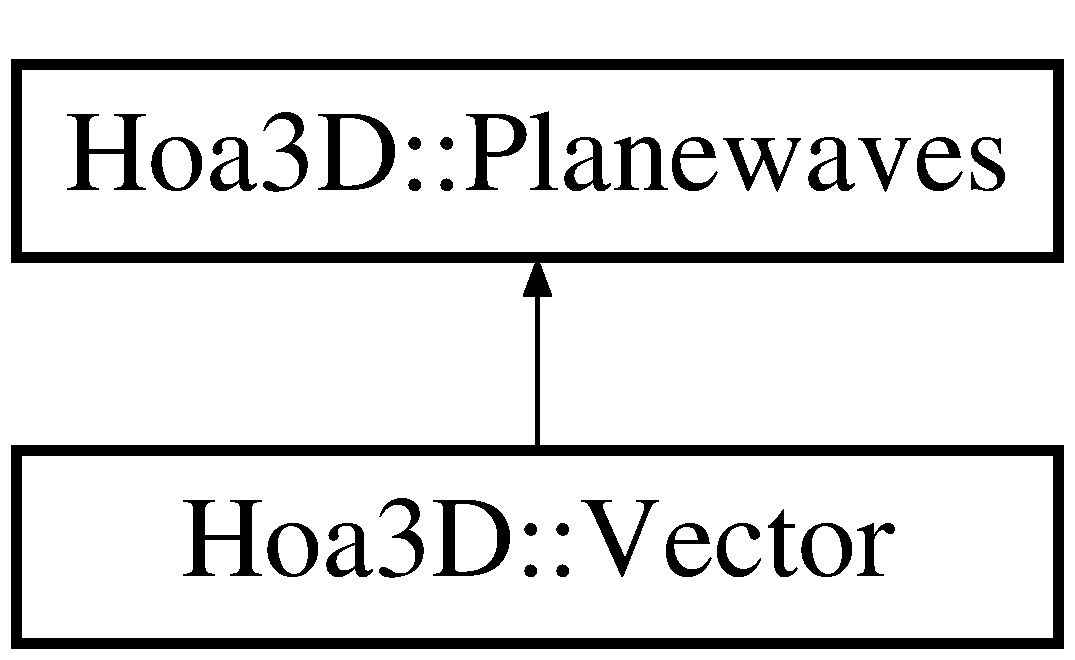
\includegraphics[height=2.000000cm]{class_hoa3_d_1_1_vector}
\end{center}
\end{figure}
\subsection*{Public Member Functions}
\begin{DoxyCompactItemize}
\item 
\hyperlink{class_hoa3_d_1_1_vector_a0a3ee9bd9477f9d20e123691c2e80315}{Vector} (unsigned int number\-Of\-Loudspeakers)
\begin{DoxyCompactList}\small\item\em The vector constructor. \end{DoxyCompactList}\item 
\hyperlink{class_hoa3_d_1_1_vector_a0f7403e0ae42fe40f54fcb35977bf95c}{$\sim$\-Vector} ()
\begin{DoxyCompactList}\small\item\em The optimization destructor. \end{DoxyCompactList}\item 
void \hyperlink{class_hoa3_d_1_1_vector_afab0f404886f74f5a139210d1a497936}{set\-Loudspeaker\-Position} (unsigned int index, double azimuth, double elevation)
\begin{DoxyCompactList}\small\item\em Set the position of a loudspeaker. \end{DoxyCompactList}\item 
void \hyperlink{class_hoa3_d_1_1_vector_a7818f4b944e66d27f08de1965c18e2bd}{process} (const float $\ast$inputs, float $\ast$outputs)
\begin{DoxyCompactList}\small\item\em This method compute the energy and velocity vectors with single precision. \end{DoxyCompactList}\item 
void \hyperlink{class_hoa3_d_1_1_vector_abf7d541dea71e683dda0aa494d843a64}{process} (const double $\ast$inputs, double $\ast$outputs)
\begin{DoxyCompactList}\small\item\em This method compute the energy and velocity vectors with double precision. \end{DoxyCompactList}\item 
void \hyperlink{class_hoa3_d_1_1_vector_a9c875cc6ac2171c5d8e1b8c1d466a844}{process\-Velocity} (const float $\ast$inputs, float $\ast$outputs)
\begin{DoxyCompactList}\small\item\em This method compute the velocity vector with single precision. \end{DoxyCompactList}\item 
void \hyperlink{class_hoa3_d_1_1_vector_a34ae72be81e72815e057e716a0f24d36}{process\-Velocity} (const double $\ast$inputs, double $\ast$outputs)
\begin{DoxyCompactList}\small\item\em This method compute the velocity vector with double precision. \end{DoxyCompactList}\item 
void \hyperlink{class_hoa3_d_1_1_vector_a7abd76a93ade46d069c922064f14c1b7}{process\-Energy} (const float $\ast$inputs, float $\ast$outputs)
\begin{DoxyCompactList}\small\item\em This method compute the energy vector with single precision. \end{DoxyCompactList}\item 
void \hyperlink{class_hoa3_d_1_1_vector_a28ad63d95b4d2c1ccabdada1955f5f96}{process\-Energy} (const double $\ast$inputs, double $\ast$outputs)
\begin{DoxyCompactList}\small\item\em This method compute the energy vector with double precision. \end{DoxyCompactList}\item 
\hyperlink{class_hoa3_d_1_1_vector_a0a3ee9bd9477f9d20e123691c2e80315}{Vector} (unsigned int number\-Of\-Loudspeakers)
\begin{DoxyCompactList}\small\item\em The vector constructor. \end{DoxyCompactList}\item 
\hyperlink{class_hoa3_d_1_1_vector_a0f7403e0ae42fe40f54fcb35977bf95c}{$\sim$\-Vector} ()
\begin{DoxyCompactList}\small\item\em The optimization destructor. \end{DoxyCompactList}\item 
void \hyperlink{class_hoa3_d_1_1_vector_afab0f404886f74f5a139210d1a497936}{set\-Loudspeaker\-Position} (unsigned int index, double azimuth, double elevation)
\begin{DoxyCompactList}\small\item\em Set the position of a loudspeaker. \end{DoxyCompactList}\item 
void \hyperlink{class_hoa3_d_1_1_vector_a7818f4b944e66d27f08de1965c18e2bd}{process} (const float $\ast$inputs, float $\ast$outputs)
\begin{DoxyCompactList}\small\item\em This method compute the energy and velocity vectors with single precision. \end{DoxyCompactList}\item 
void \hyperlink{class_hoa3_d_1_1_vector_abf7d541dea71e683dda0aa494d843a64}{process} (const double $\ast$inputs, double $\ast$outputs)
\begin{DoxyCompactList}\small\item\em This method compute the energy and velocity vectors with double precision. \end{DoxyCompactList}\item 
void \hyperlink{class_hoa3_d_1_1_vector_a9c875cc6ac2171c5d8e1b8c1d466a844}{process\-Velocity} (const float $\ast$inputs, float $\ast$outputs)
\begin{DoxyCompactList}\small\item\em This method compute the velocity vector with single precision. \end{DoxyCompactList}\item 
void \hyperlink{class_hoa3_d_1_1_vector_a34ae72be81e72815e057e716a0f24d36}{process\-Velocity} (const double $\ast$inputs, double $\ast$outputs)
\begin{DoxyCompactList}\small\item\em This method compute the velocity vector with double precision. \end{DoxyCompactList}\item 
void \hyperlink{class_hoa3_d_1_1_vector_a7abd76a93ade46d069c922064f14c1b7}{process\-Energy} (const float $\ast$inputs, float $\ast$outputs)
\begin{DoxyCompactList}\small\item\em This method compute the energy vector with single precision. \end{DoxyCompactList}\item 
void \hyperlink{class_hoa3_d_1_1_vector_a28ad63d95b4d2c1ccabdada1955f5f96}{process\-Energy} (const double $\ast$inputs, double $\ast$outputs)
\begin{DoxyCompactList}\small\item\em This method compute the energy vector with double precision. \end{DoxyCompactList}\end{DoxyCompactItemize}


\subsection{Detailed Description}
The ambisonic vector. 

The planewaves vector.

The vector class compute the energy and the velocity vector of a soudfield with signal of a spjerical set of loudspeakers. It is an useful tool to characterize the quality of the sound field resitution. For futher information \-: Michael A. Gerzon, General metatheorie of auditory localisation. Audio Engineering Society Preprint, 3306, 1992. This class retreive the cartesian coordinates of the vectors, the abscissa, the ordinate and the height. 

Definition at line 17 of file Vector.\-h.



\subsection{Constructor \& Destructor Documentation}
\hypertarget{class_hoa3_d_1_1_vector_a0a3ee9bd9477f9d20e123691c2e80315}{\index{Hoa3\-D\-::\-Vector@{Hoa3\-D\-::\-Vector}!Vector@{Vector}}
\index{Vector@{Vector}!Hoa3D::Vector@{Hoa3\-D\-::\-Vector}}
\subsubsection[{Vector}]{\setlength{\rightskip}{0pt plus 5cm}Hoa3\-D\-::\-Vector\-::\-Vector (
\begin{DoxyParamCaption}
\item[{unsigned int}]{number\-Of\-Loudspeakers}
\end{DoxyParamCaption}
)}}\label{class_hoa3_d_1_1_vector_a0a3ee9bd9477f9d20e123691c2e80315}


The vector constructor. 

The optimization constructor allocates and initialize the member values to computes vectors. The number\-Of\-Loudspeakers must be at least 1.


\begin{DoxyParams}{Parameters}
{\em number\-Of\-Loudspeakers} & The number of loudspeakers. \\
\hline
\end{DoxyParams}


Definition at line 11 of file Vector.\-cpp.

\hypertarget{class_hoa3_d_1_1_vector_a0f7403e0ae42fe40f54fcb35977bf95c}{\index{Hoa3\-D\-::\-Vector@{Hoa3\-D\-::\-Vector}!$\sim$\-Vector@{$\sim$\-Vector}}
\index{$\sim$\-Vector@{$\sim$\-Vector}!Hoa3D::Vector@{Hoa3\-D\-::\-Vector}}
\subsubsection[{$\sim$\-Vector}]{\setlength{\rightskip}{0pt plus 5cm}Hoa3\-D\-::\-Vector\-::$\sim$\-Vector (
\begin{DoxyParamCaption}
{}
\end{DoxyParamCaption}
)}}\label{class_hoa3_d_1_1_vector_a0f7403e0ae42fe40f54fcb35977bf95c}


The optimization destructor. 

The optimization destructor free the memory. 

Definition at line 151 of file Vector.\-cpp.

\hypertarget{class_hoa3_d_1_1_vector_a0a3ee9bd9477f9d20e123691c2e80315}{\index{Hoa3\-D\-::\-Vector@{Hoa3\-D\-::\-Vector}!Vector@{Vector}}
\index{Vector@{Vector}!Hoa3D::Vector@{Hoa3\-D\-::\-Vector}}
\subsubsection[{Vector}]{\setlength{\rightskip}{0pt plus 5cm}Hoa3\-D\-::\-Vector\-::\-Vector (
\begin{DoxyParamCaption}
\item[{unsigned int}]{number\-Of\-Loudspeakers}
\end{DoxyParamCaption}
)}}\label{class_hoa3_d_1_1_vector_a0a3ee9bd9477f9d20e123691c2e80315}


The vector constructor. 

The optimization constructor allocates and initialize the member values to computes vectors. The number\-Of\-Loudspeakers must be at least 1.


\begin{DoxyParams}{Parameters}
{\em number\-Of\-Loudspeakers} & The number of loudspeakers. \\
\hline
\end{DoxyParams}
\hypertarget{class_hoa3_d_1_1_vector_a0f7403e0ae42fe40f54fcb35977bf95c}{\index{Hoa3\-D\-::\-Vector@{Hoa3\-D\-::\-Vector}!$\sim$\-Vector@{$\sim$\-Vector}}
\index{$\sim$\-Vector@{$\sim$\-Vector}!Hoa3D::Vector@{Hoa3\-D\-::\-Vector}}
\subsubsection[{$\sim$\-Vector}]{\setlength{\rightskip}{0pt plus 5cm}Hoa3\-D\-::\-Vector\-::$\sim$\-Vector (
\begin{DoxyParamCaption}
{}
\end{DoxyParamCaption}
)}}\label{class_hoa3_d_1_1_vector_a0f7403e0ae42fe40f54fcb35977bf95c}


The optimization destructor. 

The optimization destructor free the memory. 

\subsection{Member Function Documentation}
\hypertarget{class_hoa3_d_1_1_vector_a7818f4b944e66d27f08de1965c18e2bd}{\index{Hoa3\-D\-::\-Vector@{Hoa3\-D\-::\-Vector}!process@{process}}
\index{process@{process}!Hoa3D::Vector@{Hoa3\-D\-::\-Vector}}
\subsubsection[{process}]{\setlength{\rightskip}{0pt plus 5cm}void Hoa3\-D\-::\-Vector\-::process (
\begin{DoxyParamCaption}
\item[{const float $\ast$}]{inputs, }
\item[{float $\ast$}]{outputs}
\end{DoxyParamCaption}
)}}\label{class_hoa3_d_1_1_vector_a7818f4b944e66d27f08de1965c18e2bd}


This method compute the energy and velocity vectors with single precision. 

You should use this method for in-\/place or not-\/in-\/place processing and compute the vectors sample by sample. The inputs array and contains the spherical harmonics samples and the minimum size must be the number of harmonics. The outputs array contains the vectors cartesian coordinates and the minimum size must be 6. The coordinates arrengement in the outputs array is velocity abscissa, velocity ordinate, velocity height, energy abscissa, energy ordinate, energy height.


\begin{DoxyParams}{Parameters}
{\em inputs} & The inputs array. \\
\hline
{\em outputs} & The outputs array. \\
\hline
\end{DoxyParams}


Definition at line 139 of file Vector.\-cpp.

\hypertarget{class_hoa3_d_1_1_vector_a7818f4b944e66d27f08de1965c18e2bd}{\index{Hoa3\-D\-::\-Vector@{Hoa3\-D\-::\-Vector}!process@{process}}
\index{process@{process}!Hoa3D::Vector@{Hoa3\-D\-::\-Vector}}
\subsubsection[{process}]{\setlength{\rightskip}{0pt plus 5cm}void Hoa3\-D\-::\-Vector\-::process (
\begin{DoxyParamCaption}
\item[{const float $\ast$}]{inputs, }
\item[{float $\ast$}]{outputs}
\end{DoxyParamCaption}
)}}\label{class_hoa3_d_1_1_vector_a7818f4b944e66d27f08de1965c18e2bd}


This method compute the energy and velocity vectors with single precision. 

You should use this method for in-\/place or not-\/in-\/place processing and compute the vectors sample by sample. The inputs array and contains the spherical harmonics samples and the minimum size must be the number of harmonics. The outputs array contains the vectors cartesian coordinates and the minimum size must be 6. The coordinates arrengement in the outputs array is velocity abscissa, velocity ordinate, velocity height, energy abscissa, energy ordinate, energy height.


\begin{DoxyParams}{Parameters}
{\em inputs} & The inputs array. \\
\hline
{\em outputs} & The outputs array. \\
\hline
\end{DoxyParams}
\hypertarget{class_hoa3_d_1_1_vector_abf7d541dea71e683dda0aa494d843a64}{\index{Hoa3\-D\-::\-Vector@{Hoa3\-D\-::\-Vector}!process@{process}}
\index{process@{process}!Hoa3D::Vector@{Hoa3\-D\-::\-Vector}}
\subsubsection[{process}]{\setlength{\rightskip}{0pt plus 5cm}void Hoa3\-D\-::\-Vector\-::process (
\begin{DoxyParamCaption}
\item[{const double $\ast$}]{inputs, }
\item[{double $\ast$}]{outputs}
\end{DoxyParamCaption}
)}}\label{class_hoa3_d_1_1_vector_abf7d541dea71e683dda0aa494d843a64}


This method compute the energy and velocity vectors with double precision. 

You should use this method for in-\/place or not-\/in-\/place processing and compute the vectors sample by sample. The inputs array and contains the spherical harmonics samples and the minimum size must be the number of harmonics. The outputs array contains the vectors cartesian coordinates and the minimum size must be 6. The coordinates arrengement in the outputs array is velocity abscissa, velocity ordinate, velocity height, energy abscissa, energy ordinate, energy height.


\begin{DoxyParams}{Parameters}
{\em inputs} & The inputs array. \\
\hline
{\em outputs} & The outputs array. \\
\hline
\end{DoxyParams}
\hypertarget{class_hoa3_d_1_1_vector_abf7d541dea71e683dda0aa494d843a64}{\index{Hoa3\-D\-::\-Vector@{Hoa3\-D\-::\-Vector}!process@{process}}
\index{process@{process}!Hoa3D::Vector@{Hoa3\-D\-::\-Vector}}
\subsubsection[{process}]{\setlength{\rightskip}{0pt plus 5cm}void Hoa3\-D\-::\-Vector\-::process (
\begin{DoxyParamCaption}
\item[{const double $\ast$}]{inputs, }
\item[{double $\ast$}]{outputs}
\end{DoxyParamCaption}
)}}\label{class_hoa3_d_1_1_vector_abf7d541dea71e683dda0aa494d843a64}


This method compute the energy and velocity vectors with double precision. 

You should use this method for in-\/place or not-\/in-\/place processing and compute the vectors sample by sample. The inputs array and contains the spherical harmonics samples and the minimum size must be the number of harmonics. The outputs array contains the vectors cartesian coordinates and the minimum size must be 6. The coordinates arrengement in the outputs array is velocity abscissa, velocity ordinate, velocity height, energy abscissa, energy ordinate, energy height.


\begin{DoxyParams}{Parameters}
{\em inputs} & The inputs array. \\
\hline
{\em outputs} & The outputs array. \\
\hline
\end{DoxyParams}


Definition at line 145 of file Vector.\-cpp.

\hypertarget{class_hoa3_d_1_1_vector_a7abd76a93ade46d069c922064f14c1b7}{\index{Hoa3\-D\-::\-Vector@{Hoa3\-D\-::\-Vector}!process\-Energy@{process\-Energy}}
\index{process\-Energy@{process\-Energy}!Hoa3D::Vector@{Hoa3\-D\-::\-Vector}}
\subsubsection[{process\-Energy}]{\setlength{\rightskip}{0pt plus 5cm}void Hoa3\-D\-::\-Vector\-::process\-Energy (
\begin{DoxyParamCaption}
\item[{const float $\ast$}]{inputs, }
\item[{float $\ast$}]{outputs}
\end{DoxyParamCaption}
)}}\label{class_hoa3_d_1_1_vector_a7abd76a93ade46d069c922064f14c1b7}


This method compute the energy vector with single precision. 

\begin{DoxyVerb}You should use this method for in-place or not-in-place processing and compute the vectors sample by sample. The inputs array and contains the spherical harmonics samples and the minimum size must be the number of harmonics. The outputs array contains the vectors cartesian coordinates and the minimum size must be 3. The coordinates arrengement in the outputs array is energy abscissa, energy ordinate, energy height.
\end{DoxyVerb}



\begin{DoxyParams}{Parameters}
{\em inputs} & The inputs array. \\
\hline
{\em outputs} & The outputs array. \\
\hline
\end{DoxyParams}
\hypertarget{class_hoa3_d_1_1_vector_a7abd76a93ade46d069c922064f14c1b7}{\index{Hoa3\-D\-::\-Vector@{Hoa3\-D\-::\-Vector}!process\-Energy@{process\-Energy}}
\index{process\-Energy@{process\-Energy}!Hoa3D::Vector@{Hoa3\-D\-::\-Vector}}
\subsubsection[{process\-Energy}]{\setlength{\rightskip}{0pt plus 5cm}void Hoa3\-D\-::\-Vector\-::process\-Energy (
\begin{DoxyParamCaption}
\item[{const float $\ast$}]{inputs, }
\item[{float $\ast$}]{outputs}
\end{DoxyParamCaption}
)}}\label{class_hoa3_d_1_1_vector_a7abd76a93ade46d069c922064f14c1b7}


This method compute the energy vector with single precision. 

\begin{DoxyVerb}You should use this method for in-place or not-in-place processing and compute the vectors sample by sample. The inputs array and contains the spherical harmonics samples and the minimum size must be the number of harmonics. The outputs array contains the vectors cartesian coordinates and the minimum size must be 3. The coordinates arrengement in the outputs array is energy abscissa, energy ordinate, energy height.
\end{DoxyVerb}



\begin{DoxyParams}{Parameters}
{\em inputs} & The inputs array. \\
\hline
{\em outputs} & The outputs array. \\
\hline
\end{DoxyParams}


Definition at line 86 of file Vector.\-cpp.

\hypertarget{class_hoa3_d_1_1_vector_a28ad63d95b4d2c1ccabdada1955f5f96}{\index{Hoa3\-D\-::\-Vector@{Hoa3\-D\-::\-Vector}!process\-Energy@{process\-Energy}}
\index{process\-Energy@{process\-Energy}!Hoa3D::Vector@{Hoa3\-D\-::\-Vector}}
\subsubsection[{process\-Energy}]{\setlength{\rightskip}{0pt plus 5cm}void Hoa3\-D\-::\-Vector\-::process\-Energy (
\begin{DoxyParamCaption}
\item[{const double $\ast$}]{inputs, }
\item[{double $\ast$}]{outputs}
\end{DoxyParamCaption}
)}}\label{class_hoa3_d_1_1_vector_a28ad63d95b4d2c1ccabdada1955f5f96}


This method compute the energy vector with double precision. 

\begin{DoxyVerb}You should use this method for in-place or not-in-place processing and compute the vectors sample by sample. The inputs array and contains the spherical harmonics samples and the minimum size must be the number of harmonics. The outputs array contains the vectors cartesian coordinates and the minimum size must be 3. The coordinates arrengement in the outputs array is energy abscissa, energy ordinate, energy height.
\end{DoxyVerb}



\begin{DoxyParams}{Parameters}
{\em inputs} & The inputs array. \\
\hline
{\em outputs} & The outputs array. \\
\hline
\end{DoxyParams}
\hypertarget{class_hoa3_d_1_1_vector_a28ad63d95b4d2c1ccabdada1955f5f96}{\index{Hoa3\-D\-::\-Vector@{Hoa3\-D\-::\-Vector}!process\-Energy@{process\-Energy}}
\index{process\-Energy@{process\-Energy}!Hoa3D::Vector@{Hoa3\-D\-::\-Vector}}
\subsubsection[{process\-Energy}]{\setlength{\rightskip}{0pt plus 5cm}void Hoa3\-D\-::\-Vector\-::process\-Energy (
\begin{DoxyParamCaption}
\item[{const double $\ast$}]{inputs, }
\item[{double $\ast$}]{outputs}
\end{DoxyParamCaption}
)}}\label{class_hoa3_d_1_1_vector_a28ad63d95b4d2c1ccabdada1955f5f96}


This method compute the energy vector with double precision. 

\begin{DoxyVerb}You should use this method for in-place or not-in-place processing and compute the vectors sample by sample. The inputs array and contains the spherical harmonics samples and the minimum size must be the number of harmonics. The outputs array contains the vectors cartesian coordinates and the minimum size must be 3. The coordinates arrengement in the outputs array is energy abscissa, energy ordinate, energy height.
\end{DoxyVerb}



\begin{DoxyParams}{Parameters}
{\em inputs} & The inputs array. \\
\hline
{\em outputs} & The outputs array. \\
\hline
\end{DoxyParams}


Definition at line 112 of file Vector.\-cpp.

\hypertarget{class_hoa3_d_1_1_vector_a9c875cc6ac2171c5d8e1b8c1d466a844}{\index{Hoa3\-D\-::\-Vector@{Hoa3\-D\-::\-Vector}!process\-Velocity@{process\-Velocity}}
\index{process\-Velocity@{process\-Velocity}!Hoa3D::Vector@{Hoa3\-D\-::\-Vector}}
\subsubsection[{process\-Velocity}]{\setlength{\rightskip}{0pt plus 5cm}void Hoa3\-D\-::\-Vector\-::process\-Velocity (
\begin{DoxyParamCaption}
\item[{const float $\ast$}]{inputs, }
\item[{float $\ast$}]{outputs}
\end{DoxyParamCaption}
)}}\label{class_hoa3_d_1_1_vector_a9c875cc6ac2171c5d8e1b8c1d466a844}


This method compute the velocity vector with single precision. 

\begin{DoxyVerb}You should use this method for in-place or not-in-place processing and compute the vectors sample by sample. The inputs array and contains the spherical harmonics samples and the minimum size must be the number of harmonics. The outputs array contains the vectors cartesian coordinates and the minimum size must be 3. The coordinates arrengement in the outputs array is velocity abscissa, velocity ordinate, velocity height.
\end{DoxyVerb}



\begin{DoxyParams}{Parameters}
{\em inputs} & The inputs array. \\
\hline
{\em outputs} & The outputs array. \\
\hline
\end{DoxyParams}


Definition at line 41 of file Vector.\-cpp.

\hypertarget{class_hoa3_d_1_1_vector_a9c875cc6ac2171c5d8e1b8c1d466a844}{\index{Hoa3\-D\-::\-Vector@{Hoa3\-D\-::\-Vector}!process\-Velocity@{process\-Velocity}}
\index{process\-Velocity@{process\-Velocity}!Hoa3D::Vector@{Hoa3\-D\-::\-Vector}}
\subsubsection[{process\-Velocity}]{\setlength{\rightskip}{0pt plus 5cm}void Hoa3\-D\-::\-Vector\-::process\-Velocity (
\begin{DoxyParamCaption}
\item[{const float $\ast$}]{inputs, }
\item[{float $\ast$}]{outputs}
\end{DoxyParamCaption}
)}}\label{class_hoa3_d_1_1_vector_a9c875cc6ac2171c5d8e1b8c1d466a844}


This method compute the velocity vector with single precision. 

\begin{DoxyVerb}You should use this method for in-place or not-in-place processing and compute the vectors sample by sample. The inputs array and contains the spherical harmonics samples and the minimum size must be the number of harmonics. The outputs array contains the vectors cartesian coordinates and the minimum size must be 3. The coordinates arrengement in the outputs array is velocity abscissa, velocity ordinate, velocity height.
\end{DoxyVerb}



\begin{DoxyParams}{Parameters}
{\em inputs} & The inputs array. \\
\hline
{\em outputs} & The outputs array. \\
\hline
\end{DoxyParams}
\hypertarget{class_hoa3_d_1_1_vector_a34ae72be81e72815e057e716a0f24d36}{\index{Hoa3\-D\-::\-Vector@{Hoa3\-D\-::\-Vector}!process\-Velocity@{process\-Velocity}}
\index{process\-Velocity@{process\-Velocity}!Hoa3D::Vector@{Hoa3\-D\-::\-Vector}}
\subsubsection[{process\-Velocity}]{\setlength{\rightskip}{0pt plus 5cm}void Hoa3\-D\-::\-Vector\-::process\-Velocity (
\begin{DoxyParamCaption}
\item[{const double $\ast$}]{inputs, }
\item[{double $\ast$}]{outputs}
\end{DoxyParamCaption}
)}}\label{class_hoa3_d_1_1_vector_a34ae72be81e72815e057e716a0f24d36}


This method compute the velocity vector with double precision. 

\begin{DoxyVerb}You should use this method for in-place or not-in-place processing and compute the vectors sample by sample. The inputs array and contains the spherical harmonics samples and the minimum size must be the number of harmonics. The outputs array contains the vectors cartesian coordinates and the minimum size must be 3. The coordinates arrengement in the outputs array is velocity abscissa, velocity ordinate, velocity height.
\end{DoxyVerb}



\begin{DoxyParams}{Parameters}
{\em inputs} & The inputs array. \\
\hline
{\em outputs} & The outputs array. \\
\hline
\end{DoxyParams}


Definition at line 64 of file Vector.\-cpp.

\hypertarget{class_hoa3_d_1_1_vector_a34ae72be81e72815e057e716a0f24d36}{\index{Hoa3\-D\-::\-Vector@{Hoa3\-D\-::\-Vector}!process\-Velocity@{process\-Velocity}}
\index{process\-Velocity@{process\-Velocity}!Hoa3D::Vector@{Hoa3\-D\-::\-Vector}}
\subsubsection[{process\-Velocity}]{\setlength{\rightskip}{0pt plus 5cm}void Hoa3\-D\-::\-Vector\-::process\-Velocity (
\begin{DoxyParamCaption}
\item[{const double $\ast$}]{inputs, }
\item[{double $\ast$}]{outputs}
\end{DoxyParamCaption}
)}}\label{class_hoa3_d_1_1_vector_a34ae72be81e72815e057e716a0f24d36}


This method compute the velocity vector with double precision. 

\begin{DoxyVerb}You should use this method for in-place or not-in-place processing and compute the vectors sample by sample. The inputs array and contains the spherical harmonics samples and the minimum size must be the number of harmonics. The outputs array contains the vectors cartesian coordinates and the minimum size must be 3. The coordinates arrengement in the outputs array is velocity abscissa, velocity ordinate, velocity height.
\end{DoxyVerb}



\begin{DoxyParams}{Parameters}
{\em inputs} & The inputs array. \\
\hline
{\em outputs} & The outputs array. \\
\hline
\end{DoxyParams}
\hypertarget{class_hoa3_d_1_1_vector_afab0f404886f74f5a139210d1a497936}{\index{Hoa3\-D\-::\-Vector@{Hoa3\-D\-::\-Vector}!set\-Loudspeaker\-Position@{set\-Loudspeaker\-Position}}
\index{set\-Loudspeaker\-Position@{set\-Loudspeaker\-Position}!Hoa3D::Vector@{Hoa3\-D\-::\-Vector}}
\subsubsection[{set\-Loudspeaker\-Position}]{\setlength{\rightskip}{0pt plus 5cm}void Hoa3\-D\-::\-Vector\-::set\-Loudspeaker\-Position (
\begin{DoxyParamCaption}
\item[{unsigned int}]{index, }
\item[{double}]{azimuth, }
\item[{double}]{elevation}
\end{DoxyParamCaption}
)}}\label{class_hoa3_d_1_1_vector_afab0f404886f74f5a139210d1a497936}


Set the position of a loudspeaker. 

Set the position of a loudspeaker with polar coordinates. The azimtuh is in radian between 0 and 2 Pi, O is the front of the soundfield and Pi is the back of the sound field. The elevation is in radian between -\/1/2 Pi and 1/2 Pi, -\/1/2 Pi the the bottom of the sound field, 0 is the center of the sound field and 1/2 Pi is the top of the sound field. The maximum index must be the number of loudspeakers -\/ 1.


\begin{DoxyParams}{Parameters}
{\em index} & The index of the loudspeaker. \\
\hline
{\em azimuth} & The azimuth. \\
\hline
{\em elevation} & The elevation. \\
\hline
\end{DoxyParams}


Definition at line 30 of file Vector.\-cpp.

\hypertarget{class_hoa3_d_1_1_vector_afab0f404886f74f5a139210d1a497936}{\index{Hoa3\-D\-::\-Vector@{Hoa3\-D\-::\-Vector}!set\-Loudspeaker\-Position@{set\-Loudspeaker\-Position}}
\index{set\-Loudspeaker\-Position@{set\-Loudspeaker\-Position}!Hoa3D::Vector@{Hoa3\-D\-::\-Vector}}
\subsubsection[{set\-Loudspeaker\-Position}]{\setlength{\rightskip}{0pt plus 5cm}void Hoa3\-D\-::\-Vector\-::set\-Loudspeaker\-Position (
\begin{DoxyParamCaption}
\item[{unsigned int}]{index, }
\item[{double}]{azimuth, }
\item[{double}]{elevation}
\end{DoxyParamCaption}
)}}\label{class_hoa3_d_1_1_vector_afab0f404886f74f5a139210d1a497936}


Set the position of a loudspeaker. 

Set the position of a loudspeaker with polar coordinates. The azimtuh is in radian between 0 and 2 Pi, O is the front of the soundfield and Pi is the back of the sound field. The elevation is in radian between -\/1/2 Pi and 1/2 Pi, -\/1/2 Pi the the bottom of the sound field, 0 is the center of the sound field and 1/2 Pi is the top of the sound field. The maximum index must be the number of loudspeakers -\/ 1.


\begin{DoxyParams}{Parameters}
{\em index} & The index of the loudspeaker. \\
\hline
{\em azimuth} & The azimuth. \\
\hline
{\em elevation} & The elevation. \\
\hline
\end{DoxyParams}


The documentation for this class was generated from the following files\-:\begin{DoxyCompactItemize}
\item 
/\-Users/\-Pierre/\-Source\-Tree/\-Hoa\-Library/\-Sources/\-Hoa2\-D/Vector.\-h\item 
/\-Users/\-Pierre/\-Source\-Tree/\-Hoa\-Library/\-Sources/\-Hoa3\-D/Vector.\-h\item 
/\-Users/\-Pierre/\-Source\-Tree/\-Hoa\-Library/\-Sources/\-Hoa2\-D/Vector.\-cpp\item 
/\-Users/\-Pierre/\-Source\-Tree/\-Hoa\-Library/\-Sources/\-Hoa3\-D/Vector.\-cpp\end{DoxyCompactItemize}

\hypertarget{class_hoa2_d_1_1_virtual_mic_manager}{\section{Hoa2\-D\-:\-:Virtual\-Mic\-Manager Class Reference}
\label{class_hoa2_d_1_1_virtual_mic_manager}\index{Hoa2\-D\-::\-Virtual\-Mic\-Manager@{Hoa2\-D\-::\-Virtual\-Mic\-Manager}}
}


The virtual microphone manager.  




{\ttfamily \#include $<$Virtual\-Mic\-Manager.\-h$>$}

\subsection*{Public Member Functions}
\begin{DoxyCompactItemize}
\item 
\hyperlink{class_hoa2_d_1_1_virtual_mic_manager_a967f0bf89c87a6c94bee641bffece3fa}{Virtual\-Mic\-Manager} (unsigned int number\-\_\-of\-\_\-mics=1)
\begin{DoxyCompactList}\small\item\em The virtual microphone manager constructor. \end{DoxyCompactList}\item 
\hyperlink{class_hoa2_d_1_1_virtual_mic_manager_a52898fb542bcdcf394e05348d27b8398}{$\sim$\-Virtual\-Mic\-Manager} ()
\begin{DoxyCompactList}\small\item\em The virtual microphone manager destructor. \end{DoxyCompactList}\item 
void \hyperlink{class_hoa2_d_1_1_virtual_mic_manager_a9bbd49d515f2dce8e515ef8341321a99}{set\-Number\-Of\-Mics} (unsigned int number\-\_\-of\-\_\-mics)
\begin{DoxyCompactList}\small\item\em Set the number of virtuals microphones you want to manage. \end{DoxyCompactList}\item 
void \hyperlink{class_hoa2_d_1_1_virtual_mic_manager_a087380cb38819e091cb76277b7cfaebb}{set\-Azimuth} (const int index, double azimuth)
\begin{DoxyCompactList}\small\item\em Set one or each virtual microphone azimuth value. \end{DoxyCompactList}\item 
void \hyperlink{class_hoa2_d_1_1_virtual_mic_manager_aeb7b3651b830d41628c0d48f94502a04}{set\-Azimuth\-List} (double $\ast$azimuths, long size)
\begin{DoxyCompactList}\small\item\em Set several virtual microphone azimuth with a list. \end{DoxyCompactList}\item 
void \hyperlink{class_hoa2_d_1_1_virtual_mic_manager_a1f0b6a97a6aebd1c0f93c0b2cd7d8653}{reset\-Azimuth} (const int index=-\/1)
\begin{DoxyCompactList}\small\item\em Reset one or each virtual microphone azimuth value. \end{DoxyCompactList}\item 
void \hyperlink{class_hoa2_d_1_1_virtual_mic_manager_ac0ebd1b76afc490cf767aa49bb7b27ba}{set\-Directivity} (const int index, const double directivity)
\begin{DoxyCompactList}\small\item\em Set one or each virtual microphone directivity value. \end{DoxyCompactList}\item 
void \hyperlink{class_hoa2_d_1_1_virtual_mic_manager_a3bc882e5ddddab304626a66078c6c8fe}{set\-Directivity\-List} (double $\ast$directivities, long size)
\begin{DoxyCompactList}\small\item\em Set several virtual microphone directivity value with a list. \end{DoxyCompactList}\item 
void \hyperlink{class_hoa2_d_1_1_virtual_mic_manager_ab37b1e4b1105a6246af9c67d1f7f3004}{reset\-Directivity} (const int index=-\/1)
\begin{DoxyCompactList}\small\item\em Reset one or each virtual microphone directivity to 1. \end{DoxyCompactList}\item 
void \hyperlink{class_hoa2_d_1_1_virtual_mic_manager_a06c95bbe7df88f3b21e7a82593a1a6aa}{set\-Selected} (const int index, int selected\-State)
\begin{DoxyCompactList}\small\item\em Set the selected state of one or each virtual microphone. \end{DoxyCompactList}\item 
void \hyperlink{class_hoa2_d_1_1_virtual_mic_manager_a7d03540e436756e59a26dd8747c47f8d}{rotate\-Selected\-Mics} (double new\-Radian, int source\-Being\-Dragged, int magnet=0)
\begin{DoxyCompactList}\small\item\em \hyperlink{class_hoa2_d_1_1_rotate}{Rotate} all of the currently selected microphones relative to one microphone azimuth rotation. \end{DoxyCompactList}\item 
void \hyperlink{class_hoa2_d_1_1_virtual_mic_manager_a1031b56d2f7bfc4a40ff5d5f478ae9a6}{set\-Fisheye\-Dest\-Azimuth} (double azimuth)
\begin{DoxyCompactList}\small\item\em Set fisheye destination azimuth. \end{DoxyCompactList}\item 
void \hyperlink{class_hoa2_d_1_1_virtual_mic_manager_ad41d6ca6482278a16e7121fc37b8f005}{set\-Fisheye\-Start\-Azimuth} (const int index)
\begin{DoxyCompactList}\small\item\em Set the fisheye start azimuth of one or several microphone with current azimuth. \end{DoxyCompactList}\item 
void \hyperlink{class_hoa2_d_1_1_virtual_mic_manager_a6351bacf0f305122062df4f69b7be6ee}{set\-Fisheye\-Start\-Azimuth} (const int index, double radian)
\begin{DoxyCompactList}\small\item\em Set the fisheye start azimuth of one or several microphone. \end{DoxyCompactList}\item 
void \hyperlink{class_hoa2_d_1_1_virtual_mic_manager_a8a470cb0bed6a99d97ed535717de3432}{set\-Fisheye\-Step\-With\-Delta} (const int index, double delta)
\begin{DoxyCompactList}\small\item\em Increment or decrement the fisheye step by a value. \end{DoxyCompactList}\item 
void \hyperlink{class_hoa2_d_1_1_virtual_mic_manager_a53cc4adb53136e44bed715e13ba5b834}{set\-Fisheye\-Step\-Direct} (const int index, double fisheye\-Step)
\begin{DoxyCompactList}\small\item\em Set the fisheye step directly. \end{DoxyCompactList}\item 
void \hyperlink{class_hoa2_d_1_1_virtual_mic_manager_af6543c15a67dffd32b66cfb5ba9d7d12}{set\-Azimuth\-To\-Closest\-Def\-Mic\-Azimuth} (const int index)
\begin{DoxyCompactList}\small\item\em Set virtual microphone azimuth value to the closest default azimuth position value. \end{DoxyCompactList}\item 
long \hyperlink{class_hoa2_d_1_1_virtual_mic_manager_ad410ea735c2d90d55d7e438d3527ef57}{get\-Number\-Of\-Selected\-Mics} ()
\begin{DoxyCompactList}\small\item\em Retrieve the number of selected microphones. \end{DoxyCompactList}\item 
double \hyperlink{class_hoa2_d_1_1_virtual_mic_manager_aab43c873ac5968e3c2023ee2b0ce2e24}{get\-Closest\-Def\-Mic\-Azimuth} (const int index)
\begin{DoxyCompactList}\small\item\em Retrieve the closest default azimuth position of a virtual microphone. \end{DoxyCompactList}\item 
double \hyperlink{class_hoa2_d_1_1_virtual_mic_manager_a5e055290edf0b236927a057836463bfe}{get\-Closest\-Def\-Mic\-Azimuth} (double azimuth)
\begin{DoxyCompactList}\small\item\em Retrieve the closest default azimuth position relative to an azimuth value. \end{DoxyCompactList}\item 
double \hyperlink{class_hoa2_d_1_1_virtual_mic_manager_a6e6ad752d94fad0fb1c6ad014bdf29fb}{get\-Closest\-Def\-Mic\-Distance} (const int index)
\begin{DoxyCompactList}\small\item\em Retrieve the distance to the closest default azimuth position relative to the azimuth of a virtual microphone. \end{DoxyCompactList}\item 
double \hyperlink{class_hoa2_d_1_1_virtual_mic_manager_af7eacde3002e30fc45eda1a2133a1e6e}{get\-Closest\-Def\-Mic\-Distance} (double azimuth)
\begin{DoxyCompactList}\small\item\em Retrieve the distance to the closest default azimuth position relative to an azimuth value. \end{DoxyCompactList}\item 
double \hyperlink{class_hoa2_d_1_1_virtual_mic_manager_ae811a1625b2698dc3229281fe0dd361e}{get\-Fisheye\-Dest\-Azimuth} () const 
\begin{DoxyCompactList}\small\item\em Retrieve the fisheye destination azimuth value. \end{DoxyCompactList}\item 
long \hyperlink{class_hoa2_d_1_1_virtual_mic_manager_accfd94e543f908e703cabd4829c42ae0}{get\-Number\-Of\-Mics} () const 
\begin{DoxyCompactList}\small\item\em Retrieve the number of virtual microphones currently managed. \end{DoxyCompactList}\item 
double \hyperlink{class_hoa2_d_1_1_virtual_mic_manager_a8d211940759074053682e1ca119f05fd}{get\-Fisheye\-Step} () const 
\begin{DoxyCompactList}\small\item\em Retrieve the current fisheye step. \end{DoxyCompactList}\item 
bool \hyperlink{class_hoa2_d_1_1_virtual_mic_manager_a81228c748207a601761eee6c2c999c31}{is\-Selected} (const int index) const 
\begin{DoxyCompactList}\small\item\em Retrieve the selection state of a virtual microphone. \end{DoxyCompactList}\item 
double \hyperlink{class_hoa2_d_1_1_virtual_mic_manager_add79d3cfea68de215e2be864d302a19c}{get\-Directivity} (const int index) const 
\begin{DoxyCompactList}\small\item\em Retrieve the directivity value of a virtual microphone. \end{DoxyCompactList}\item 
double \hyperlink{class_hoa2_d_1_1_virtual_mic_manager_ae01486ff891cd4e6e3951beed0680d81}{get\-Fisheye\-Start\-Azimuth} (const int index) const 
\begin{DoxyCompactList}\small\item\em Retrieve the fisheye start azimuth value of a virtual microphone. \end{DoxyCompactList}\item 
double \hyperlink{class_hoa2_d_1_1_virtual_mic_manager_a641578b9c0a40bde63de09228dd03f84}{get\-Abscissa} (const int index) const 
\begin{DoxyCompactList}\small\item\em Retrieve the abscissa of a virtual microphone. \end{DoxyCompactList}\item 
double \hyperlink{class_hoa2_d_1_1_virtual_mic_manager_a5ef17b2bbb91282caeb002818de38e6e}{get\-Ordinate} (const int index) const 
\begin{DoxyCompactList}\small\item\em Retrieve the ordinate of a virtual microphone. \end{DoxyCompactList}\item 
double \hyperlink{class_hoa2_d_1_1_virtual_mic_manager_a4b279c16b6c2f49710153f2f5345d926}{get\-Azimuth} (const int index) const 
\begin{DoxyCompactList}\small\item\em Retrieve the azimuth of a virtual microphone. \end{DoxyCompactList}\end{DoxyCompactItemize}


\subsection{Detailed Description}
The virtual microphone manager. 

The virtual microphone manager should be used to manage a group of virtual microphones. 

Definition at line 17 of file Virtual\-Mic\-Manager.\-h.



\subsection{Constructor \& Destructor Documentation}
\hypertarget{class_hoa2_d_1_1_virtual_mic_manager_a967f0bf89c87a6c94bee641bffece3fa}{\index{Hoa2\-D\-::\-Virtual\-Mic\-Manager@{Hoa2\-D\-::\-Virtual\-Mic\-Manager}!Virtual\-Mic\-Manager@{Virtual\-Mic\-Manager}}
\index{Virtual\-Mic\-Manager@{Virtual\-Mic\-Manager}!Hoa2D::VirtualMicManager@{Hoa2\-D\-::\-Virtual\-Mic\-Manager}}
\subsubsection[{Virtual\-Mic\-Manager}]{\setlength{\rightskip}{0pt plus 5cm}Hoa2\-D\-::\-Virtual\-Mic\-Manager\-::\-Virtual\-Mic\-Manager (
\begin{DoxyParamCaption}
\item[{unsigned int}]{number\-\_\-of\-\_\-mics = {\ttfamily 1}}
\end{DoxyParamCaption}
)}}\label{class_hoa2_d_1_1_virtual_mic_manager_a967f0bf89c87a6c94bee641bffece3fa}


The virtual microphone manager constructor. 

\begin{DoxyVerb}The virtual microphone manager constructor allocates and initialize the member values for each virtual microphone.
\end{DoxyVerb}



\begin{DoxyParams}{Parameters}
{\em number\-\_\-of\-\_\-mics} & The number of virtual microphones you need to manage, default is 1. \\
\hline
\end{DoxyParams}


Definition at line 11 of file Virtual\-Mic\-Manager.\-cpp.

\hypertarget{class_hoa2_d_1_1_virtual_mic_manager_a52898fb542bcdcf394e05348d27b8398}{\index{Hoa2\-D\-::\-Virtual\-Mic\-Manager@{Hoa2\-D\-::\-Virtual\-Mic\-Manager}!$\sim$\-Virtual\-Mic\-Manager@{$\sim$\-Virtual\-Mic\-Manager}}
\index{$\sim$\-Virtual\-Mic\-Manager@{$\sim$\-Virtual\-Mic\-Manager}!Hoa2D::VirtualMicManager@{Hoa2\-D\-::\-Virtual\-Mic\-Manager}}
\subsubsection[{$\sim$\-Virtual\-Mic\-Manager}]{\setlength{\rightskip}{0pt plus 5cm}Hoa2\-D\-::\-Virtual\-Mic\-Manager\-::$\sim$\-Virtual\-Mic\-Manager (
\begin{DoxyParamCaption}
{}
\end{DoxyParamCaption}
)}}\label{class_hoa2_d_1_1_virtual_mic_manager_a52898fb542bcdcf394e05348d27b8398}


The virtual microphone manager destructor. 

The virtual microphone manager destructor free the memory. 

Definition at line 17 of file Virtual\-Mic\-Manager.\-cpp.



\subsection{Member Function Documentation}
\hypertarget{class_hoa2_d_1_1_virtual_mic_manager_a641578b9c0a40bde63de09228dd03f84}{\index{Hoa2\-D\-::\-Virtual\-Mic\-Manager@{Hoa2\-D\-::\-Virtual\-Mic\-Manager}!get\-Abscissa@{get\-Abscissa}}
\index{get\-Abscissa@{get\-Abscissa}!Hoa2D::VirtualMicManager@{Hoa2\-D\-::\-Virtual\-Mic\-Manager}}
\subsubsection[{get\-Abscissa}]{\setlength{\rightskip}{0pt plus 5cm}double Hoa2\-D\-::\-Virtual\-Mic\-Manager\-::get\-Abscissa (
\begin{DoxyParamCaption}
\item[{const int}]{index}
\end{DoxyParamCaption}
) const\hspace{0.3cm}{\ttfamily [inline]}}}\label{class_hoa2_d_1_1_virtual_mic_manager_a641578b9c0a40bde63de09228dd03f84}


Retrieve the abscissa of a virtual microphone. 


\begin{DoxyParams}{Parameters}
{\em index} & The index of the microphone. \\
\hline
\end{DoxyParams}
\begin{DoxyReturn}{Returns}
The abscissa of the virtual microphone. 
\end{DoxyReturn}


Definition at line 291 of file Virtual\-Mic\-Manager.\-h.

\hypertarget{class_hoa2_d_1_1_virtual_mic_manager_a4b279c16b6c2f49710153f2f5345d926}{\index{Hoa2\-D\-::\-Virtual\-Mic\-Manager@{Hoa2\-D\-::\-Virtual\-Mic\-Manager}!get\-Azimuth@{get\-Azimuth}}
\index{get\-Azimuth@{get\-Azimuth}!Hoa2D::VirtualMicManager@{Hoa2\-D\-::\-Virtual\-Mic\-Manager}}
\subsubsection[{get\-Azimuth}]{\setlength{\rightskip}{0pt plus 5cm}double Hoa2\-D\-::\-Virtual\-Mic\-Manager\-::get\-Azimuth (
\begin{DoxyParamCaption}
\item[{const int}]{index}
\end{DoxyParamCaption}
) const\hspace{0.3cm}{\ttfamily [inline]}}}\label{class_hoa2_d_1_1_virtual_mic_manager_a4b279c16b6c2f49710153f2f5345d926}


Retrieve the azimuth of a virtual microphone. 


\begin{DoxyParams}{Parameters}
{\em index} & The index of the microphone. \\
\hline
\end{DoxyParams}
\begin{DoxyReturn}{Returns}
The azimuth of the virtual microphone. 
\end{DoxyReturn}
\begin{DoxySeeAlso}{See Also}
\hyperlink{class_hoa2_d_1_1_virtual_mic_manager_a087380cb38819e091cb76277b7cfaebb}{set\-Azimuth} 
\end{DoxySeeAlso}


Definition at line 306 of file Virtual\-Mic\-Manager.\-h.

\hypertarget{class_hoa2_d_1_1_virtual_mic_manager_aab43c873ac5968e3c2023ee2b0ce2e24}{\index{Hoa2\-D\-::\-Virtual\-Mic\-Manager@{Hoa2\-D\-::\-Virtual\-Mic\-Manager}!get\-Closest\-Def\-Mic\-Azimuth@{get\-Closest\-Def\-Mic\-Azimuth}}
\index{get\-Closest\-Def\-Mic\-Azimuth@{get\-Closest\-Def\-Mic\-Azimuth}!Hoa2D::VirtualMicManager@{Hoa2\-D\-::\-Virtual\-Mic\-Manager}}
\subsubsection[{get\-Closest\-Def\-Mic\-Azimuth}]{\setlength{\rightskip}{0pt plus 5cm}double Hoa2\-D\-::\-Virtual\-Mic\-Manager\-::get\-Closest\-Def\-Mic\-Azimuth (
\begin{DoxyParamCaption}
\item[{const int}]{index}
\end{DoxyParamCaption}
)}}\label{class_hoa2_d_1_1_virtual_mic_manager_aab43c873ac5968e3c2023ee2b0ce2e24}


Retrieve the closest default azimuth position of a virtual microphone. 


\begin{DoxyParams}{Parameters}
{\em index} & The index of the microphone. \\
\hline
\end{DoxyParams}
\begin{DoxyReturn}{Returns}
closest default azimuth position of the virtual microphone. 
\end{DoxyReturn}
\begin{DoxySeeAlso}{See Also}
\hyperlink{class_hoa2_d_1_1_virtual_mic_manager_a6e6ad752d94fad0fb1c6ad014bdf29fb}{get\-Closest\-Def\-Mic\-Distance} 
\end{DoxySeeAlso}


Definition at line 243 of file Virtual\-Mic\-Manager.\-cpp.

\hypertarget{class_hoa2_d_1_1_virtual_mic_manager_a5e055290edf0b236927a057836463bfe}{\index{Hoa2\-D\-::\-Virtual\-Mic\-Manager@{Hoa2\-D\-::\-Virtual\-Mic\-Manager}!get\-Closest\-Def\-Mic\-Azimuth@{get\-Closest\-Def\-Mic\-Azimuth}}
\index{get\-Closest\-Def\-Mic\-Azimuth@{get\-Closest\-Def\-Mic\-Azimuth}!Hoa2D::VirtualMicManager@{Hoa2\-D\-::\-Virtual\-Mic\-Manager}}
\subsubsection[{get\-Closest\-Def\-Mic\-Azimuth}]{\setlength{\rightskip}{0pt plus 5cm}double Hoa2\-D\-::\-Virtual\-Mic\-Manager\-::get\-Closest\-Def\-Mic\-Azimuth (
\begin{DoxyParamCaption}
\item[{double}]{azimuth}
\end{DoxyParamCaption}
)}}\label{class_hoa2_d_1_1_virtual_mic_manager_a5e055290edf0b236927a057836463bfe}


Retrieve the closest default azimuth position relative to an azimuth value. 


\begin{DoxyParams}{Parameters}
{\em azimuth} & The relative azimuth. \\
\hline
\end{DoxyParams}
\begin{DoxyReturn}{Returns}
The closest default azimuth position of the virtual microphone relative to the azimuth value you passed in. 
\end{DoxyReturn}
\begin{DoxySeeAlso}{See Also}
\hyperlink{class_hoa2_d_1_1_virtual_mic_manager_a6e6ad752d94fad0fb1c6ad014bdf29fb}{get\-Closest\-Def\-Mic\-Distance} 
\end{DoxySeeAlso}


Definition at line 248 of file Virtual\-Mic\-Manager.\-cpp.

\hypertarget{class_hoa2_d_1_1_virtual_mic_manager_a6e6ad752d94fad0fb1c6ad014bdf29fb}{\index{Hoa2\-D\-::\-Virtual\-Mic\-Manager@{Hoa2\-D\-::\-Virtual\-Mic\-Manager}!get\-Closest\-Def\-Mic\-Distance@{get\-Closest\-Def\-Mic\-Distance}}
\index{get\-Closest\-Def\-Mic\-Distance@{get\-Closest\-Def\-Mic\-Distance}!Hoa2D::VirtualMicManager@{Hoa2\-D\-::\-Virtual\-Mic\-Manager}}
\subsubsection[{get\-Closest\-Def\-Mic\-Distance}]{\setlength{\rightskip}{0pt plus 5cm}double Hoa2\-D\-::\-Virtual\-Mic\-Manager\-::get\-Closest\-Def\-Mic\-Distance (
\begin{DoxyParamCaption}
\item[{const int}]{index}
\end{DoxyParamCaption}
)}}\label{class_hoa2_d_1_1_virtual_mic_manager_a6e6ad752d94fad0fb1c6ad014bdf29fb}


Retrieve the distance to the closest default azimuth position relative to the azimuth of a virtual microphone. 


\begin{DoxyParams}{Parameters}
{\em index} & The index of the microphone. \\
\hline
\end{DoxyParams}
\begin{DoxyReturn}{Returns}
The distance to the closest default azimuth position. 
\end{DoxyReturn}
\begin{DoxySeeAlso}{See Also}
\hyperlink{class_hoa2_d_1_1_virtual_mic_manager_aab43c873ac5968e3c2023ee2b0ce2e24}{get\-Closest\-Def\-Mic\-Azimuth} 
\end{DoxySeeAlso}


Definition at line 267 of file Virtual\-Mic\-Manager.\-cpp.

\hypertarget{class_hoa2_d_1_1_virtual_mic_manager_af7eacde3002e30fc45eda1a2133a1e6e}{\index{Hoa2\-D\-::\-Virtual\-Mic\-Manager@{Hoa2\-D\-::\-Virtual\-Mic\-Manager}!get\-Closest\-Def\-Mic\-Distance@{get\-Closest\-Def\-Mic\-Distance}}
\index{get\-Closest\-Def\-Mic\-Distance@{get\-Closest\-Def\-Mic\-Distance}!Hoa2D::VirtualMicManager@{Hoa2\-D\-::\-Virtual\-Mic\-Manager}}
\subsubsection[{get\-Closest\-Def\-Mic\-Distance}]{\setlength{\rightskip}{0pt plus 5cm}double Hoa2\-D\-::\-Virtual\-Mic\-Manager\-::get\-Closest\-Def\-Mic\-Distance (
\begin{DoxyParamCaption}
\item[{double}]{azimuth}
\end{DoxyParamCaption}
)}}\label{class_hoa2_d_1_1_virtual_mic_manager_af7eacde3002e30fc45eda1a2133a1e6e}


Retrieve the distance to the closest default azimuth position relative to an azimuth value. 


\begin{DoxyParams}{Parameters}
{\em azimuth} & The relative azimuth. \\
\hline
\end{DoxyParams}
\begin{DoxyReturn}{Returns}
The distance to the closest default azimuth position of the virtual microphone relative to the azimuth value you passed in. 
\end{DoxyReturn}
\begin{DoxySeeAlso}{See Also}
\hyperlink{class_hoa2_d_1_1_virtual_mic_manager_aab43c873ac5968e3c2023ee2b0ce2e24}{get\-Closest\-Def\-Mic\-Azimuth} 
\end{DoxySeeAlso}


Definition at line 272 of file Virtual\-Mic\-Manager.\-cpp.

\hypertarget{class_hoa2_d_1_1_virtual_mic_manager_add79d3cfea68de215e2be864d302a19c}{\index{Hoa2\-D\-::\-Virtual\-Mic\-Manager@{Hoa2\-D\-::\-Virtual\-Mic\-Manager}!get\-Directivity@{get\-Directivity}}
\index{get\-Directivity@{get\-Directivity}!Hoa2D::VirtualMicManager@{Hoa2\-D\-::\-Virtual\-Mic\-Manager}}
\subsubsection[{get\-Directivity}]{\setlength{\rightskip}{0pt plus 5cm}double Hoa2\-D\-::\-Virtual\-Mic\-Manager\-::get\-Directivity (
\begin{DoxyParamCaption}
\item[{const int}]{index}
\end{DoxyParamCaption}
) const\hspace{0.3cm}{\ttfamily [inline]}}}\label{class_hoa2_d_1_1_virtual_mic_manager_add79d3cfea68de215e2be864d302a19c}


Retrieve the directivity value of a virtual microphone. 


\begin{DoxyParams}{Parameters}
{\em index} & The index of the microphone. \\
\hline
\end{DoxyParams}
\begin{DoxyReturn}{Returns}
The directivity value of the virtual microphone. 
\end{DoxyReturn}
\begin{DoxySeeAlso}{See Also}
\hyperlink{class_hoa2_d_1_1_virtual_mic_manager_ac0ebd1b76afc490cf767aa49bb7b27ba}{set\-Directivity} 
\end{DoxySeeAlso}


Definition at line 276 of file Virtual\-Mic\-Manager.\-h.

\hypertarget{class_hoa2_d_1_1_virtual_mic_manager_ae811a1625b2698dc3229281fe0dd361e}{\index{Hoa2\-D\-::\-Virtual\-Mic\-Manager@{Hoa2\-D\-::\-Virtual\-Mic\-Manager}!get\-Fisheye\-Dest\-Azimuth@{get\-Fisheye\-Dest\-Azimuth}}
\index{get\-Fisheye\-Dest\-Azimuth@{get\-Fisheye\-Dest\-Azimuth}!Hoa2D::VirtualMicManager@{Hoa2\-D\-::\-Virtual\-Mic\-Manager}}
\subsubsection[{get\-Fisheye\-Dest\-Azimuth}]{\setlength{\rightskip}{0pt plus 5cm}double Hoa2\-D\-::\-Virtual\-Mic\-Manager\-::get\-Fisheye\-Dest\-Azimuth (
\begin{DoxyParamCaption}
{}
\end{DoxyParamCaption}
) const\hspace{0.3cm}{\ttfamily [inline]}}}\label{class_hoa2_d_1_1_virtual_mic_manager_ae811a1625b2698dc3229281fe0dd361e}


Retrieve the fisheye destination azimuth value. 

\begin{DoxyReturn}{Returns}
The fisheye destination azimuth value. 
\end{DoxyReturn}
\begin{DoxySeeAlso}{See Also}
\hyperlink{class_hoa2_d_1_1_virtual_mic_manager_a1031b56d2f7bfc4a40ff5d5f478ae9a6}{set\-Fisheye\-Dest\-Azimuth} 
\end{DoxySeeAlso}


Definition at line 246 of file Virtual\-Mic\-Manager.\-h.

\hypertarget{class_hoa2_d_1_1_virtual_mic_manager_ae01486ff891cd4e6e3951beed0680d81}{\index{Hoa2\-D\-::\-Virtual\-Mic\-Manager@{Hoa2\-D\-::\-Virtual\-Mic\-Manager}!get\-Fisheye\-Start\-Azimuth@{get\-Fisheye\-Start\-Azimuth}}
\index{get\-Fisheye\-Start\-Azimuth@{get\-Fisheye\-Start\-Azimuth}!Hoa2D::VirtualMicManager@{Hoa2\-D\-::\-Virtual\-Mic\-Manager}}
\subsubsection[{get\-Fisheye\-Start\-Azimuth}]{\setlength{\rightskip}{0pt plus 5cm}double Hoa2\-D\-::\-Virtual\-Mic\-Manager\-::get\-Fisheye\-Start\-Azimuth (
\begin{DoxyParamCaption}
\item[{const int}]{index}
\end{DoxyParamCaption}
) const\hspace{0.3cm}{\ttfamily [inline]}}}\label{class_hoa2_d_1_1_virtual_mic_manager_ae01486ff891cd4e6e3951beed0680d81}


Retrieve the fisheye start azimuth value of a virtual microphone. 


\begin{DoxyParams}{Parameters}
{\em index} & The index of the microphone. \\
\hline
\end{DoxyParams}
\begin{DoxyReturn}{Returns}
The fisheye start azimuth value of the virtual microphone. 
\end{DoxyReturn}
\begin{DoxySeeAlso}{See Also}
\hyperlink{class_hoa2_d_1_1_virtual_mic_manager_ad41d6ca6482278a16e7121fc37b8f005}{set\-Fisheye\-Start\-Azimuth} 
\end{DoxySeeAlso}


Definition at line 284 of file Virtual\-Mic\-Manager.\-h.

\hypertarget{class_hoa2_d_1_1_virtual_mic_manager_a8d211940759074053682e1ca119f05fd}{\index{Hoa2\-D\-::\-Virtual\-Mic\-Manager@{Hoa2\-D\-::\-Virtual\-Mic\-Manager}!get\-Fisheye\-Step@{get\-Fisheye\-Step}}
\index{get\-Fisheye\-Step@{get\-Fisheye\-Step}!Hoa2D::VirtualMicManager@{Hoa2\-D\-::\-Virtual\-Mic\-Manager}}
\subsubsection[{get\-Fisheye\-Step}]{\setlength{\rightskip}{0pt plus 5cm}double Hoa2\-D\-::\-Virtual\-Mic\-Manager\-::get\-Fisheye\-Step (
\begin{DoxyParamCaption}
{}
\end{DoxyParamCaption}
) const\hspace{0.3cm}{\ttfamily [inline]}}}\label{class_hoa2_d_1_1_virtual_mic_manager_a8d211940759074053682e1ca119f05fd}


Retrieve the current fisheye step. 

\begin{DoxyReturn}{Returns}
The current fisheye step. 
\end{DoxyReturn}
\begin{DoxySeeAlso}{See Also}
\hyperlink{class_hoa2_d_1_1_virtual_mic_manager_a53cc4adb53136e44bed715e13ba5b834}{set\-Fisheye\-Step\-Direct}, \hyperlink{class_hoa2_d_1_1_virtual_mic_manager_a8a470cb0bed6a99d97ed535717de3432}{set\-Fisheye\-Step\-With\-Delta} 
\end{DoxySeeAlso}


Definition at line 260 of file Virtual\-Mic\-Manager.\-h.

\hypertarget{class_hoa2_d_1_1_virtual_mic_manager_accfd94e543f908e703cabd4829c42ae0}{\index{Hoa2\-D\-::\-Virtual\-Mic\-Manager@{Hoa2\-D\-::\-Virtual\-Mic\-Manager}!get\-Number\-Of\-Mics@{get\-Number\-Of\-Mics}}
\index{get\-Number\-Of\-Mics@{get\-Number\-Of\-Mics}!Hoa2D::VirtualMicManager@{Hoa2\-D\-::\-Virtual\-Mic\-Manager}}
\subsubsection[{get\-Number\-Of\-Mics}]{\setlength{\rightskip}{0pt plus 5cm}long Hoa2\-D\-::\-Virtual\-Mic\-Manager\-::get\-Number\-Of\-Mics (
\begin{DoxyParamCaption}
{}
\end{DoxyParamCaption}
) const\hspace{0.3cm}{\ttfamily [inline]}}}\label{class_hoa2_d_1_1_virtual_mic_manager_accfd94e543f908e703cabd4829c42ae0}


Retrieve the number of virtual microphones currently managed. 

\begin{DoxyReturn}{Returns}
The number of virtual microphones currently managed. 
\end{DoxyReturn}
\begin{DoxySeeAlso}{See Also}
\hyperlink{class_hoa2_d_1_1_virtual_mic_manager_a9bbd49d515f2dce8e515ef8341321a99}{set\-Number\-Of\-Mics} 
\end{DoxySeeAlso}


Definition at line 253 of file Virtual\-Mic\-Manager.\-h.

\hypertarget{class_hoa2_d_1_1_virtual_mic_manager_ad410ea735c2d90d55d7e438d3527ef57}{\index{Hoa2\-D\-::\-Virtual\-Mic\-Manager@{Hoa2\-D\-::\-Virtual\-Mic\-Manager}!get\-Number\-Of\-Selected\-Mics@{get\-Number\-Of\-Selected\-Mics}}
\index{get\-Number\-Of\-Selected\-Mics@{get\-Number\-Of\-Selected\-Mics}!Hoa2D::VirtualMicManager@{Hoa2\-D\-::\-Virtual\-Mic\-Manager}}
\subsubsection[{get\-Number\-Of\-Selected\-Mics}]{\setlength{\rightskip}{0pt plus 5cm}long Hoa2\-D\-::\-Virtual\-Mic\-Manager\-::get\-Number\-Of\-Selected\-Mics (
\begin{DoxyParamCaption}
{}
\end{DoxyParamCaption}
)}}\label{class_hoa2_d_1_1_virtual_mic_manager_ad410ea735c2d90d55d7e438d3527ef57}


Retrieve the number of selected microphones. 

\begin{DoxyReturn}{Returns}
The number of selected microphones. 
\end{DoxyReturn}
\begin{DoxySeeAlso}{See Also}
\hyperlink{class_hoa2_d_1_1_virtual_mic_manager_a06c95bbe7df88f3b21e7a82593a1a6aa}{set\-Selected} 
\end{DoxySeeAlso}


Definition at line 289 of file Virtual\-Mic\-Manager.\-cpp.

\hypertarget{class_hoa2_d_1_1_virtual_mic_manager_a5ef17b2bbb91282caeb002818de38e6e}{\index{Hoa2\-D\-::\-Virtual\-Mic\-Manager@{Hoa2\-D\-::\-Virtual\-Mic\-Manager}!get\-Ordinate@{get\-Ordinate}}
\index{get\-Ordinate@{get\-Ordinate}!Hoa2D::VirtualMicManager@{Hoa2\-D\-::\-Virtual\-Mic\-Manager}}
\subsubsection[{get\-Ordinate}]{\setlength{\rightskip}{0pt plus 5cm}double Hoa2\-D\-::\-Virtual\-Mic\-Manager\-::get\-Ordinate (
\begin{DoxyParamCaption}
\item[{const int}]{index}
\end{DoxyParamCaption}
) const\hspace{0.3cm}{\ttfamily [inline]}}}\label{class_hoa2_d_1_1_virtual_mic_manager_a5ef17b2bbb91282caeb002818de38e6e}


Retrieve the ordinate of a virtual microphone. 


\begin{DoxyParams}{Parameters}
{\em index} & The index of the microphone. \\
\hline
\end{DoxyParams}
\begin{DoxyReturn}{Returns}
The ordinate of the virtual microphone. 
\end{DoxyReturn}


Definition at line 298 of file Virtual\-Mic\-Manager.\-h.

\hypertarget{class_hoa2_d_1_1_virtual_mic_manager_a81228c748207a601761eee6c2c999c31}{\index{Hoa2\-D\-::\-Virtual\-Mic\-Manager@{Hoa2\-D\-::\-Virtual\-Mic\-Manager}!is\-Selected@{is\-Selected}}
\index{is\-Selected@{is\-Selected}!Hoa2D::VirtualMicManager@{Hoa2\-D\-::\-Virtual\-Mic\-Manager}}
\subsubsection[{is\-Selected}]{\setlength{\rightskip}{0pt plus 5cm}bool Hoa2\-D\-::\-Virtual\-Mic\-Manager\-::is\-Selected (
\begin{DoxyParamCaption}
\item[{const int}]{index}
\end{DoxyParamCaption}
) const\hspace{0.3cm}{\ttfamily [inline]}}}\label{class_hoa2_d_1_1_virtual_mic_manager_a81228c748207a601761eee6c2c999c31}


Retrieve the selection state of a virtual microphone. 


\begin{DoxyParams}{Parameters}
{\em index} & The index of the microphone. \\
\hline
\end{DoxyParams}
\begin{DoxyReturn}{Returns}
The selection state of the virtual microphone. 
\end{DoxyReturn}
\begin{DoxySeeAlso}{See Also}
\hyperlink{class_hoa2_d_1_1_virtual_mic_manager_a06c95bbe7df88f3b21e7a82593a1a6aa}{set\-Selected} 
\end{DoxySeeAlso}


Definition at line 268 of file Virtual\-Mic\-Manager.\-h.

\hypertarget{class_hoa2_d_1_1_virtual_mic_manager_a1f0b6a97a6aebd1c0f93c0b2cd7d8653}{\index{Hoa2\-D\-::\-Virtual\-Mic\-Manager@{Hoa2\-D\-::\-Virtual\-Mic\-Manager}!reset\-Azimuth@{reset\-Azimuth}}
\index{reset\-Azimuth@{reset\-Azimuth}!Hoa2D::VirtualMicManager@{Hoa2\-D\-::\-Virtual\-Mic\-Manager}}
\subsubsection[{reset\-Azimuth}]{\setlength{\rightskip}{0pt plus 5cm}void Hoa2\-D\-::\-Virtual\-Mic\-Manager\-::reset\-Azimuth (
\begin{DoxyParamCaption}
\item[{const int}]{index = {\ttfamily -\/1}}
\end{DoxyParamCaption}
)}}\label{class_hoa2_d_1_1_virtual_mic_manager_a1f0b6a97a6aebd1c0f93c0b2cd7d8653}


Reset one or each virtual microphone azimuth value. 

\begin{DoxyVerb}Reset one or each virtual microphone to the default azimuth value.
\end{DoxyVerb}
 If you want to reset all of the microphones azimuth value, pass -\/1 in the index parameter.


\begin{DoxyParams}{Parameters}
{\em index} & The index of the microphone (pass -\/1 to reset all of them). \\
\hline
\end{DoxyParams}
\begin{DoxySeeAlso}{See Also}
\hyperlink{class_hoa2_d_1_1_virtual_mic_manager_a087380cb38819e091cb76277b7cfaebb}{set\-Azimuth}, \hyperlink{class_hoa2_d_1_1_virtual_mic_manager_aeb7b3651b830d41628c0d48f94502a04}{set\-Azimuth\-List} 
\end{DoxySeeAlso}


Definition at line 56 of file Virtual\-Mic\-Manager.\-cpp.

\hypertarget{class_hoa2_d_1_1_virtual_mic_manager_ab37b1e4b1105a6246af9c67d1f7f3004}{\index{Hoa2\-D\-::\-Virtual\-Mic\-Manager@{Hoa2\-D\-::\-Virtual\-Mic\-Manager}!reset\-Directivity@{reset\-Directivity}}
\index{reset\-Directivity@{reset\-Directivity}!Hoa2D::VirtualMicManager@{Hoa2\-D\-::\-Virtual\-Mic\-Manager}}
\subsubsection[{reset\-Directivity}]{\setlength{\rightskip}{0pt plus 5cm}void Hoa2\-D\-::\-Virtual\-Mic\-Manager\-::reset\-Directivity (
\begin{DoxyParamCaption}
\item[{const int}]{index = {\ttfamily -\/1}}
\end{DoxyParamCaption}
)}}\label{class_hoa2_d_1_1_virtual_mic_manager_ab37b1e4b1105a6246af9c67d1f7f3004}


Reset one or each virtual microphone directivity to 1. 

If you want to reset all of the microphones directivity value, pass -\/1 in the index parameter.


\begin{DoxyParams}{Parameters}
{\em index} & The index of the microphone (pass -\/1 to reset all of them). \\
\hline
\end{DoxyParams}
\begin{DoxySeeAlso}{See Also}
\hyperlink{class_hoa2_d_1_1_virtual_mic_manager_ac0ebd1b76afc490cf767aa49bb7b27ba}{set\-Directivity}, \hyperlink{class_hoa2_d_1_1_virtual_mic_manager_a3bc882e5ddddab304626a66078c6c8fe}{set\-Directivity\-List} 
\end{DoxySeeAlso}


Definition at line 67 of file Virtual\-Mic\-Manager.\-cpp.

\hypertarget{class_hoa2_d_1_1_virtual_mic_manager_a7d03540e436756e59a26dd8747c47f8d}{\index{Hoa2\-D\-::\-Virtual\-Mic\-Manager@{Hoa2\-D\-::\-Virtual\-Mic\-Manager}!rotate\-Selected\-Mics@{rotate\-Selected\-Mics}}
\index{rotate\-Selected\-Mics@{rotate\-Selected\-Mics}!Hoa2D::VirtualMicManager@{Hoa2\-D\-::\-Virtual\-Mic\-Manager}}
\subsubsection[{rotate\-Selected\-Mics}]{\setlength{\rightskip}{0pt plus 5cm}void Hoa2\-D\-::\-Virtual\-Mic\-Manager\-::rotate\-Selected\-Mics (
\begin{DoxyParamCaption}
\item[{double}]{new\-Radian, }
\item[{int}]{source\-Being\-Dragged, }
\item[{int}]{magnet = {\ttfamily 0}}
\end{DoxyParamCaption}
)}}\label{class_hoa2_d_1_1_virtual_mic_manager_a7d03540e436756e59a26dd8747c47f8d}


\hyperlink{class_hoa2_d_1_1_rotate}{Rotate} all of the currently selected microphones relative to one microphone azimuth rotation. 


\begin{DoxyParams}{Parameters}
{\em new\-Radian} & The new azimuth of the source which is being dragged \\
\hline
{\em source\-Being\-Dragged} & The index of the microphone which is being dragged. \\
\hline
{\em magnet} & Pass 1 to magnetize the microphone to one of the default azimuth positions \\
\hline
\end{DoxyParams}


Definition at line 123 of file Virtual\-Mic\-Manager.\-cpp.

\hypertarget{class_hoa2_d_1_1_virtual_mic_manager_a087380cb38819e091cb76277b7cfaebb}{\index{Hoa2\-D\-::\-Virtual\-Mic\-Manager@{Hoa2\-D\-::\-Virtual\-Mic\-Manager}!set\-Azimuth@{set\-Azimuth}}
\index{set\-Azimuth@{set\-Azimuth}!Hoa2D::VirtualMicManager@{Hoa2\-D\-::\-Virtual\-Mic\-Manager}}
\subsubsection[{set\-Azimuth}]{\setlength{\rightskip}{0pt plus 5cm}void Hoa2\-D\-::\-Virtual\-Mic\-Manager\-::set\-Azimuth (
\begin{DoxyParamCaption}
\item[{const int}]{index, }
\item[{double}]{azimuth}
\end{DoxyParamCaption}
)}}\label{class_hoa2_d_1_1_virtual_mic_manager_a087380cb38819e091cb76277b7cfaebb}


Set one or each virtual microphone azimuth value. 

If you want to reset all of the microphones azimuth value, pass -\/1 in the index parameter.


\begin{DoxyParams}{Parameters}
{\em index} & The index of the microphone (pass -\/1 to reset all of them). \\
\hline
{\em azimuth} & The new azimuth value in radians. \\
\hline
\end{DoxyParams}
\begin{DoxySeeAlso}{See Also}
\hyperlink{class_hoa2_d_1_1_virtual_mic_manager_a1f0b6a97a6aebd1c0f93c0b2cd7d8653}{reset\-Azimuth}, \hyperlink{class_hoa2_d_1_1_virtual_mic_manager_aeb7b3651b830d41628c0d48f94502a04}{set\-Azimuth\-List} 
\end{DoxySeeAlso}


Definition at line 84 of file Virtual\-Mic\-Manager.\-cpp.

\hypertarget{class_hoa2_d_1_1_virtual_mic_manager_aeb7b3651b830d41628c0d48f94502a04}{\index{Hoa2\-D\-::\-Virtual\-Mic\-Manager@{Hoa2\-D\-::\-Virtual\-Mic\-Manager}!set\-Azimuth\-List@{set\-Azimuth\-List}}
\index{set\-Azimuth\-List@{set\-Azimuth\-List}!Hoa2D::VirtualMicManager@{Hoa2\-D\-::\-Virtual\-Mic\-Manager}}
\subsubsection[{set\-Azimuth\-List}]{\setlength{\rightskip}{0pt plus 5cm}void Hoa2\-D\-::\-Virtual\-Mic\-Manager\-::set\-Azimuth\-List (
\begin{DoxyParamCaption}
\item[{double $\ast$}]{azimuths, }
\item[{long}]{size}
\end{DoxyParamCaption}
)}}\label{class_hoa2_d_1_1_virtual_mic_manager_aeb7b3651b830d41628c0d48f94502a04}


Set several virtual microphone azimuth with a list. 


\begin{DoxyParams}{Parameters}
{\em azimuths} & An array of azimuth values in radians. \\
\hline
{\em size} & The size of the array. \\
\hline
\end{DoxyParams}
\begin{DoxySeeAlso}{See Also}
\hyperlink{class_hoa2_d_1_1_virtual_mic_manager_a087380cb38819e091cb76277b7cfaebb}{set\-Azimuth}, \hyperlink{class_hoa2_d_1_1_virtual_mic_manager_ac0ebd1b76afc490cf767aa49bb7b27ba}{set\-Directivity} 
\end{DoxySeeAlso}


Definition at line 78 of file Virtual\-Mic\-Manager.\-cpp.

\hypertarget{class_hoa2_d_1_1_virtual_mic_manager_af6543c15a67dffd32b66cfb5ba9d7d12}{\index{Hoa2\-D\-::\-Virtual\-Mic\-Manager@{Hoa2\-D\-::\-Virtual\-Mic\-Manager}!set\-Azimuth\-To\-Closest\-Def\-Mic\-Azimuth@{set\-Azimuth\-To\-Closest\-Def\-Mic\-Azimuth}}
\index{set\-Azimuth\-To\-Closest\-Def\-Mic\-Azimuth@{set\-Azimuth\-To\-Closest\-Def\-Mic\-Azimuth}!Hoa2D::VirtualMicManager@{Hoa2\-D\-::\-Virtual\-Mic\-Manager}}
\subsubsection[{set\-Azimuth\-To\-Closest\-Def\-Mic\-Azimuth}]{\setlength{\rightskip}{0pt plus 5cm}void Hoa2\-D\-::\-Virtual\-Mic\-Manager\-::set\-Azimuth\-To\-Closest\-Def\-Mic\-Azimuth (
\begin{DoxyParamCaption}
\item[{const int}]{index}
\end{DoxyParamCaption}
)}}\label{class_hoa2_d_1_1_virtual_mic_manager_af6543c15a67dffd32b66cfb5ba9d7d12}


Set virtual microphone azimuth value to the closest default azimuth position value. 


\begin{DoxyParams}{Parameters}
{\em index} & The index of the microphone. \\
\hline
\end{DoxyParams}
\begin{DoxySeeAlso}{See Also}
\hyperlink{class_hoa2_d_1_1_virtual_mic_manager_a1f0b6a97a6aebd1c0f93c0b2cd7d8653}{reset\-Azimuth}, \hyperlink{class_hoa2_d_1_1_virtual_mic_manager_a087380cb38819e091cb76277b7cfaebb}{set\-Azimuth} 
\end{DoxySeeAlso}


Definition at line 283 of file Virtual\-Mic\-Manager.\-cpp.

\hypertarget{class_hoa2_d_1_1_virtual_mic_manager_ac0ebd1b76afc490cf767aa49bb7b27ba}{\index{Hoa2\-D\-::\-Virtual\-Mic\-Manager@{Hoa2\-D\-::\-Virtual\-Mic\-Manager}!set\-Directivity@{set\-Directivity}}
\index{set\-Directivity@{set\-Directivity}!Hoa2D::VirtualMicManager@{Hoa2\-D\-::\-Virtual\-Mic\-Manager}}
\subsubsection[{set\-Directivity}]{\setlength{\rightskip}{0pt plus 5cm}void Hoa2\-D\-::\-Virtual\-Mic\-Manager\-::set\-Directivity (
\begin{DoxyParamCaption}
\item[{const int}]{index, }
\item[{const double}]{directivity}
\end{DoxyParamCaption}
)}}\label{class_hoa2_d_1_1_virtual_mic_manager_ac0ebd1b76afc490cf767aa49bb7b27ba}


Set one or each virtual microphone directivity value. 

If you want to reset all of the microphones azimuth value, pass -\/1 in the index parameter.


\begin{DoxyParams}{Parameters}
{\em index} & The index of the microphone (pass -\/1 to reset all of them). \\
\hline
{\em directivity} & The new directivity value (between 0 and 1). \\
\hline
\end{DoxyParams}
\begin{DoxySeeAlso}{See Also}
\hyperlink{class_hoa2_d_1_1_virtual_mic_manager_ab37b1e4b1105a6246af9c67d1f7f3004}{reset\-Directivity}, \hyperlink{class_hoa2_d_1_1_virtual_mic_manager_a3bc882e5ddddab304626a66078c6c8fe}{set\-Directivity\-List} 
\end{DoxySeeAlso}


Definition at line 101 of file Virtual\-Mic\-Manager.\-cpp.

\hypertarget{class_hoa2_d_1_1_virtual_mic_manager_a3bc882e5ddddab304626a66078c6c8fe}{\index{Hoa2\-D\-::\-Virtual\-Mic\-Manager@{Hoa2\-D\-::\-Virtual\-Mic\-Manager}!set\-Directivity\-List@{set\-Directivity\-List}}
\index{set\-Directivity\-List@{set\-Directivity\-List}!Hoa2D::VirtualMicManager@{Hoa2\-D\-::\-Virtual\-Mic\-Manager}}
\subsubsection[{set\-Directivity\-List}]{\setlength{\rightskip}{0pt plus 5cm}void Hoa2\-D\-::\-Virtual\-Mic\-Manager\-::set\-Directivity\-List (
\begin{DoxyParamCaption}
\item[{double $\ast$}]{directivities, }
\item[{long}]{size}
\end{DoxyParamCaption}
)}}\label{class_hoa2_d_1_1_virtual_mic_manager_a3bc882e5ddddab304626a66078c6c8fe}


Set several virtual microphone directivity value with a list. 


\begin{DoxyParams}{Parameters}
{\em directivities} & An array of directivity (between 0 and 1). \\
\hline
{\em size} & The size of the array. \\
\hline
\end{DoxyParams}
\begin{DoxySeeAlso}{See Also}
\hyperlink{class_hoa2_d_1_1_virtual_mic_manager_ac0ebd1b76afc490cf767aa49bb7b27ba}{set\-Directivity}, \hyperlink{class_hoa2_d_1_1_virtual_mic_manager_ab37b1e4b1105a6246af9c67d1f7f3004}{reset\-Directivity} 
\end{DoxySeeAlso}


Definition at line 95 of file Virtual\-Mic\-Manager.\-cpp.

\hypertarget{class_hoa2_d_1_1_virtual_mic_manager_a1031b56d2f7bfc4a40ff5d5f478ae9a6}{\index{Hoa2\-D\-::\-Virtual\-Mic\-Manager@{Hoa2\-D\-::\-Virtual\-Mic\-Manager}!set\-Fisheye\-Dest\-Azimuth@{set\-Fisheye\-Dest\-Azimuth}}
\index{set\-Fisheye\-Dest\-Azimuth@{set\-Fisheye\-Dest\-Azimuth}!Hoa2D::VirtualMicManager@{Hoa2\-D\-::\-Virtual\-Mic\-Manager}}
\subsubsection[{set\-Fisheye\-Dest\-Azimuth}]{\setlength{\rightskip}{0pt plus 5cm}void Hoa2\-D\-::\-Virtual\-Mic\-Manager\-::set\-Fisheye\-Dest\-Azimuth (
\begin{DoxyParamCaption}
\item[{double}]{azimuth}
\end{DoxyParamCaption}
)}}\label{class_hoa2_d_1_1_virtual_mic_manager_a1031b56d2f7bfc4a40ff5d5f478ae9a6}


Set fisheye destination azimuth. 


\begin{DoxyParams}{Parameters}
{\em azimuth} & The azimuth value of the fisheye destination in radians. \\
\hline
\end{DoxyParams}
\begin{DoxySeeAlso}{See Also}
\hyperlink{class_hoa2_d_1_1_virtual_mic_manager_ae811a1625b2698dc3229281fe0dd361e}{get\-Fisheye\-Dest\-Azimuth}, \hyperlink{class_hoa2_d_1_1_virtual_mic_manager_ad41d6ca6482278a16e7121fc37b8f005}{set\-Fisheye\-Start\-Azimuth} 
\end{DoxySeeAlso}


Definition at line 153 of file Virtual\-Mic\-Manager.\-cpp.

\hypertarget{class_hoa2_d_1_1_virtual_mic_manager_ad41d6ca6482278a16e7121fc37b8f005}{\index{Hoa2\-D\-::\-Virtual\-Mic\-Manager@{Hoa2\-D\-::\-Virtual\-Mic\-Manager}!set\-Fisheye\-Start\-Azimuth@{set\-Fisheye\-Start\-Azimuth}}
\index{set\-Fisheye\-Start\-Azimuth@{set\-Fisheye\-Start\-Azimuth}!Hoa2D::VirtualMicManager@{Hoa2\-D\-::\-Virtual\-Mic\-Manager}}
\subsubsection[{set\-Fisheye\-Start\-Azimuth}]{\setlength{\rightskip}{0pt plus 5cm}void Hoa2\-D\-::\-Virtual\-Mic\-Manager\-::set\-Fisheye\-Start\-Azimuth (
\begin{DoxyParamCaption}
\item[{const int}]{index}
\end{DoxyParamCaption}
)}}\label{class_hoa2_d_1_1_virtual_mic_manager_ad41d6ca6482278a16e7121fc37b8f005}


Set the fisheye start azimuth of one or several microphone with current azimuth. 


\begin{DoxyParams}{Parameters}
{\em index} & The index of the microphone if greather than -\/1, pass -\/2 to affect all selected microphones, pass -\/1 to affect all microphones \\
\hline
\end{DoxyParams}
\begin{DoxySeeAlso}{See Also}

\end{DoxySeeAlso}


Definition at line 184 of file Virtual\-Mic\-Manager.\-cpp.

\hypertarget{class_hoa2_d_1_1_virtual_mic_manager_a6351bacf0f305122062df4f69b7be6ee}{\index{Hoa2\-D\-::\-Virtual\-Mic\-Manager@{Hoa2\-D\-::\-Virtual\-Mic\-Manager}!set\-Fisheye\-Start\-Azimuth@{set\-Fisheye\-Start\-Azimuth}}
\index{set\-Fisheye\-Start\-Azimuth@{set\-Fisheye\-Start\-Azimuth}!Hoa2D::VirtualMicManager@{Hoa2\-D\-::\-Virtual\-Mic\-Manager}}
\subsubsection[{set\-Fisheye\-Start\-Azimuth}]{\setlength{\rightskip}{0pt plus 5cm}void Hoa2\-D\-::\-Virtual\-Mic\-Manager\-::set\-Fisheye\-Start\-Azimuth (
\begin{DoxyParamCaption}
\item[{const int}]{index, }
\item[{double}]{radian}
\end{DoxyParamCaption}
)}}\label{class_hoa2_d_1_1_virtual_mic_manager_a6351bacf0f305122062df4f69b7be6ee}


Set the fisheye start azimuth of one or several microphone. 


\begin{DoxyParams}{Parameters}
{\em index} & The index of the microphone if greather than -\/1, pass -\/2 to affect all selected microphones, pass -\/1 to affect all microphones \\
\hline
\end{DoxyParams}


Definition at line 201 of file Virtual\-Mic\-Manager.\-cpp.

\hypertarget{class_hoa2_d_1_1_virtual_mic_manager_a53cc4adb53136e44bed715e13ba5b834}{\index{Hoa2\-D\-::\-Virtual\-Mic\-Manager@{Hoa2\-D\-::\-Virtual\-Mic\-Manager}!set\-Fisheye\-Step\-Direct@{set\-Fisheye\-Step\-Direct}}
\index{set\-Fisheye\-Step\-Direct@{set\-Fisheye\-Step\-Direct}!Hoa2D::VirtualMicManager@{Hoa2\-D\-::\-Virtual\-Mic\-Manager}}
\subsubsection[{set\-Fisheye\-Step\-Direct}]{\setlength{\rightskip}{0pt plus 5cm}void Hoa2\-D\-::\-Virtual\-Mic\-Manager\-::set\-Fisheye\-Step\-Direct (
\begin{DoxyParamCaption}
\item[{const int}]{index, }
\item[{double}]{fisheye\-Step}
\end{DoxyParamCaption}
)}}\label{class_hoa2_d_1_1_virtual_mic_manager_a53cc4adb53136e44bed715e13ba5b834}


Set the fisheye step directly. 


\begin{DoxyParams}{Parameters}
{\em index} & The index of the microphone if greather than -\/1, pass -\/2 to affect all selected microphones, pass -\/1 to affect all microphones \\
\hline
{\em fisheye\-Step} & The fisheye step (between 0 and 1). \\
\hline
\end{DoxyParams}
\begin{DoxySeeAlso}{See Also}
\hyperlink{class_hoa2_d_1_1_virtual_mic_manager_a8a470cb0bed6a99d97ed535717de3432}{set\-Fisheye\-Step\-With\-Delta} 
\end{DoxySeeAlso}


Definition at line 165 of file Virtual\-Mic\-Manager.\-cpp.

\hypertarget{class_hoa2_d_1_1_virtual_mic_manager_a8a470cb0bed6a99d97ed535717de3432}{\index{Hoa2\-D\-::\-Virtual\-Mic\-Manager@{Hoa2\-D\-::\-Virtual\-Mic\-Manager}!set\-Fisheye\-Step\-With\-Delta@{set\-Fisheye\-Step\-With\-Delta}}
\index{set\-Fisheye\-Step\-With\-Delta@{set\-Fisheye\-Step\-With\-Delta}!Hoa2D::VirtualMicManager@{Hoa2\-D\-::\-Virtual\-Mic\-Manager}}
\subsubsection[{set\-Fisheye\-Step\-With\-Delta}]{\setlength{\rightskip}{0pt plus 5cm}void Hoa2\-D\-::\-Virtual\-Mic\-Manager\-::set\-Fisheye\-Step\-With\-Delta (
\begin{DoxyParamCaption}
\item[{const int}]{index, }
\item[{double}]{delta}
\end{DoxyParamCaption}
)}}\label{class_hoa2_d_1_1_virtual_mic_manager_a8a470cb0bed6a99d97ed535717de3432}


Increment or decrement the fisheye step by a value. 


\begin{DoxyParams}{Parameters}
{\em index} & The index of the microphone if greather than -\/1, pass -\/2 to affect all selected microphones, pass -\/1 to affect all microphones \\
\hline
\end{DoxyParams}
\begin{DoxySeeAlso}{See Also}
\hyperlink{class_hoa2_d_1_1_virtual_mic_manager_a53cc4adb53136e44bed715e13ba5b834}{set\-Fisheye\-Step\-Direct} 
\end{DoxySeeAlso}


Definition at line 159 of file Virtual\-Mic\-Manager.\-cpp.

\hypertarget{class_hoa2_d_1_1_virtual_mic_manager_a9bbd49d515f2dce8e515ef8341321a99}{\index{Hoa2\-D\-::\-Virtual\-Mic\-Manager@{Hoa2\-D\-::\-Virtual\-Mic\-Manager}!set\-Number\-Of\-Mics@{set\-Number\-Of\-Mics}}
\index{set\-Number\-Of\-Mics@{set\-Number\-Of\-Mics}!Hoa2D::VirtualMicManager@{Hoa2\-D\-::\-Virtual\-Mic\-Manager}}
\subsubsection[{set\-Number\-Of\-Mics}]{\setlength{\rightskip}{0pt plus 5cm}void Hoa2\-D\-::\-Virtual\-Mic\-Manager\-::set\-Number\-Of\-Mics (
\begin{DoxyParamCaption}
\item[{unsigned int}]{number\-\_\-of\-\_\-mics}
\end{DoxyParamCaption}
)}}\label{class_hoa2_d_1_1_virtual_mic_manager_a9bbd49d515f2dce8e515ef8341321a99}


Set the number of virtuals microphones you want to manage. 


\begin{DoxyParams}{Parameters}
{\em number\-\_\-of\-\_\-mics} & The number of virtual microphones you need to manage, default is 1. \\
\hline
\end{DoxyParams}


Definition at line 24 of file Virtual\-Mic\-Manager.\-cpp.

\hypertarget{class_hoa2_d_1_1_virtual_mic_manager_a06c95bbe7df88f3b21e7a82593a1a6aa}{\index{Hoa2\-D\-::\-Virtual\-Mic\-Manager@{Hoa2\-D\-::\-Virtual\-Mic\-Manager}!set\-Selected@{set\-Selected}}
\index{set\-Selected@{set\-Selected}!Hoa2D::VirtualMicManager@{Hoa2\-D\-::\-Virtual\-Mic\-Manager}}
\subsubsection[{set\-Selected}]{\setlength{\rightskip}{0pt plus 5cm}void Hoa2\-D\-::\-Virtual\-Mic\-Manager\-::set\-Selected (
\begin{DoxyParamCaption}
\item[{const int}]{index, }
\item[{int}]{selected\-State}
\end{DoxyParamCaption}
)}}\label{class_hoa2_d_1_1_virtual_mic_manager_a06c95bbe7df88f3b21e7a82593a1a6aa}


Set the selected state of one or each virtual microphone. 

If you want to reset all of the microphones selected state, pass -\/1 in the index parameter.


\begin{DoxyParams}{Parameters}
{\em index} & The index of the microphone (pass -\/1 to reset all of them). \\
\hline
{\em selected\-State} & The selected state, pass 0 to unselect, 1 to select and -\/1 to toggle the state. \\
\hline
\end{DoxyParams}
\begin{DoxySeeAlso}{See Also}
\hyperlink{class_hoa2_d_1_1_virtual_mic_manager_ad410ea735c2d90d55d7e438d3527ef57}{get\-Number\-Of\-Selected\-Mics} 
\end{DoxySeeAlso}


Definition at line 112 of file Virtual\-Mic\-Manager.\-cpp.



The documentation for this class was generated from the following files\-:\begin{DoxyCompactItemize}
\item 
/\-Users/elioton/\-Documents/programmation/\-C\-I\-C\-M/source\-Tree/\-Hoa\-Library/\-Sources/\-Hoa2\-D/Virtual\-Mic\-Manager.\-h\item 
/\-Users/elioton/\-Documents/programmation/\-C\-I\-C\-M/source\-Tree/\-Hoa\-Library/\-Sources/\-Hoa2\-D/Virtual\-Mic\-Manager.\-cpp\end{DoxyCompactItemize}

\hypertarget{class_hoa2_d_1_1_wider}{\section{Hoa2\-D\-:\-:Wider Class Reference}
\label{class_hoa2_d_1_1_wider}\index{Hoa2\-D\-::\-Wider@{Hoa2\-D\-::\-Wider}}
}


The ambisonic wider.  




{\ttfamily \#include $<$Wider.\-h$>$}

Inheritance diagram for Hoa2\-D\-:\-:Wider\-:\begin{figure}[H]
\begin{center}
\leavevmode
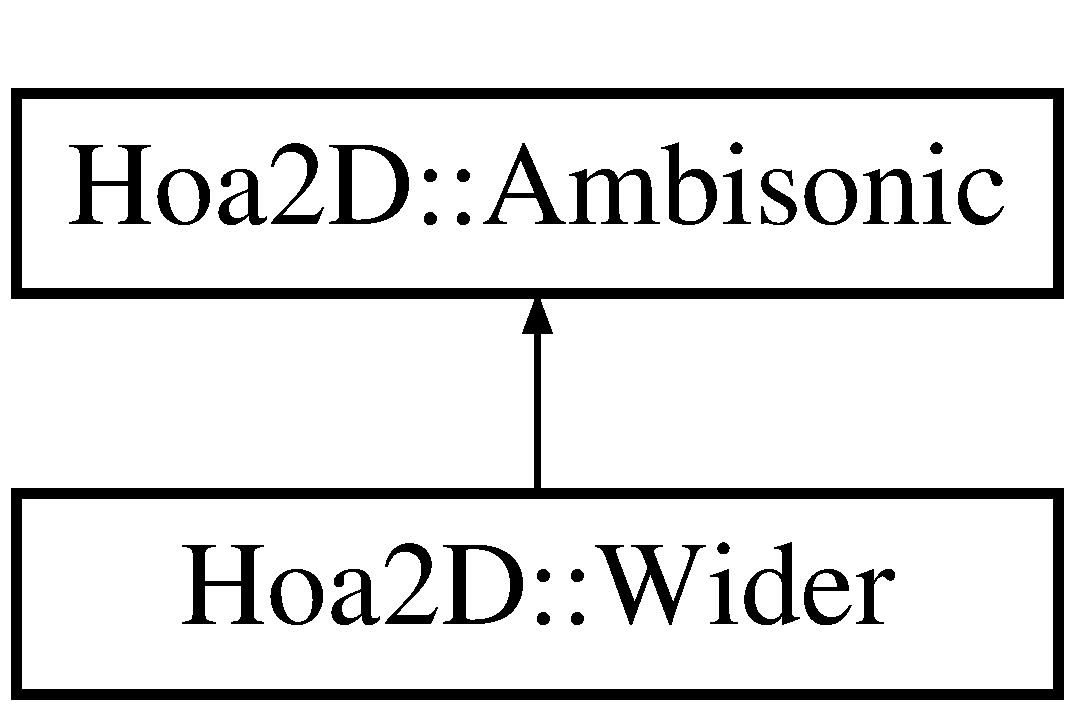
\includegraphics[height=2.000000cm]{class_hoa2_d_1_1_wider}
\end{center}
\end{figure}
\subsection*{Public Member Functions}
\begin{DoxyCompactItemize}
\item 
\hyperlink{class_hoa2_d_1_1_wider_a847bbdfd81f552b4b246276582519e9a}{Wider} (unsigned int order)
\begin{DoxyCompactList}\small\item\em The wider constructor. \end{DoxyCompactList}\item 
\hyperlink{class_hoa2_d_1_1_wider_a350dd3e9918f7fdaa977fe5c56db98d1}{$\sim$\-Wider} ()
\begin{DoxyCompactList}\small\item\em The wider destructor. \end{DoxyCompactList}\item 
void \hyperlink{class_hoa2_d_1_1_wider_af43a64e22d453bd5bf6f2d46013fe758}{set\-Widening\-Value} (const double value)
\begin{DoxyCompactList}\small\item\em This method set the widening value. \end{DoxyCompactList}\item 
double \hyperlink{class_hoa2_d_1_1_wider_a6de242ad21bc1197433b23b746e73c8b}{get\-Widening\-Value} () const 
\begin{DoxyCompactList}\small\item\em This method retreive the widening value. \end{DoxyCompactList}\item 
void \hyperlink{class_hoa2_d_1_1_wider_a5183122d315e15a73e5cfe709914e72d}{process} (const float $\ast$inputs, float $\ast$outputs)
\begin{DoxyCompactList}\small\item\em This method performs the widening with single precision. \end{DoxyCompactList}\item 
void \hyperlink{class_hoa2_d_1_1_wider_a40ed4da484d0cac0a730d4eec723327e}{process} (const double $\ast$inputs, double $\ast$outputs)
\begin{DoxyCompactList}\small\item\em This method performs the widening with double precision. \end{DoxyCompactList}\end{DoxyCompactItemize}


\subsection{Detailed Description}
The ambisonic wider. 

The wider should be used to widen the sound propagation with fractional order simulution. The sound field precision depends to the decomposition order. The zero decomposition order has 1 omnidirectionnal harmonic and all the sounds seem to come from all the directions. While the order increases, the number of harmonics increases, the lobes of an encoded sounds narrow and the origin of the sounds is more accurate. Then fractional order can be used to decrease the sound field precision and to wide the sound field propagation. 

Definition at line 17 of file Wider.\-h.



\subsection{Constructor \& Destructor Documentation}
\hypertarget{class_hoa2_d_1_1_wider_a847bbdfd81f552b4b246276582519e9a}{\index{Hoa2\-D\-::\-Wider@{Hoa2\-D\-::\-Wider}!Wider@{Wider}}
\index{Wider@{Wider}!Hoa2D::Wider@{Hoa2\-D\-::\-Wider}}
\subsubsection[{Wider}]{\setlength{\rightskip}{0pt plus 5cm}Hoa2\-D\-::\-Wider\-::\-Wider (
\begin{DoxyParamCaption}
\item[{unsigned int}]{order}
\end{DoxyParamCaption}
)}}\label{class_hoa2_d_1_1_wider_a847bbdfd81f552b4b246276582519e9a}


The wider constructor. 

The wider constructor allocates and initialize the member values to computes circular harmonics weighted coefficients depending of a decomposition order. The order must be at least 1.


\begin{DoxyParams}{Parameters}
{\em order} & The order. \\
\hline
\end{DoxyParams}


Definition at line 11 of file Wider.\-cpp.

\hypertarget{class_hoa2_d_1_1_wider_a350dd3e9918f7fdaa977fe5c56db98d1}{\index{Hoa2\-D\-::\-Wider@{Hoa2\-D\-::\-Wider}!$\sim$\-Wider@{$\sim$\-Wider}}
\index{$\sim$\-Wider@{$\sim$\-Wider}!Hoa2D::Wider@{Hoa2\-D\-::\-Wider}}
\subsubsection[{$\sim$\-Wider}]{\setlength{\rightskip}{0pt plus 5cm}Hoa2\-D\-::\-Wider\-::$\sim$\-Wider (
\begin{DoxyParamCaption}
{}
\end{DoxyParamCaption}
)}}\label{class_hoa2_d_1_1_wider_a350dd3e9918f7fdaa977fe5c56db98d1}


The wider destructor. 

The wider destructor free the memory. 

Definition at line 64 of file Wider.\-cpp.



\subsection{Member Function Documentation}
\hypertarget{class_hoa2_d_1_1_wider_a6de242ad21bc1197433b23b746e73c8b}{\index{Hoa2\-D\-::\-Wider@{Hoa2\-D\-::\-Wider}!get\-Widening\-Value@{get\-Widening\-Value}}
\index{get\-Widening\-Value@{get\-Widening\-Value}!Hoa2D::Wider@{Hoa2\-D\-::\-Wider}}
\subsubsection[{get\-Widening\-Value}]{\setlength{\rightskip}{0pt plus 5cm}double Hoa2\-D\-::\-Wider\-::get\-Widening\-Value (
\begin{DoxyParamCaption}
{}
\end{DoxyParamCaption}
) const\hspace{0.3cm}{\ttfamily [inline]}}}\label{class_hoa2_d_1_1_wider_a6de242ad21bc1197433b23b746e73c8b}


This method retreive the widening value. 

The method returns the widening value.

\begin{DoxyReturn}{Returns}
The widening value. 
\end{DoxyReturn}


Definition at line 50 of file Wider.\-h.

\hypertarget{class_hoa2_d_1_1_wider_a5183122d315e15a73e5cfe709914e72d}{\index{Hoa2\-D\-::\-Wider@{Hoa2\-D\-::\-Wider}!process@{process}}
\index{process@{process}!Hoa2D::Wider@{Hoa2\-D\-::\-Wider}}
\subsubsection[{process}]{\setlength{\rightskip}{0pt plus 5cm}void Hoa2\-D\-::\-Wider\-::process (
\begin{DoxyParamCaption}
\item[{const float $\ast$}]{inputs, }
\item[{float $\ast$}]{outputs}
\end{DoxyParamCaption}
)}}\label{class_hoa2_d_1_1_wider_a5183122d315e15a73e5cfe709914e72d}


This method performs the widening with single precision. 

You should use this method for in-\/place or not-\/in-\/place processing and performs the widening sample by sample. The inputs array and outputs array contains the circular harmonics samples and the minimum size must be the number of harmonics.


\begin{DoxyParams}{Parameters}
{\em inputs} & The inputs array. \\
\hline
{\em outputs} & The outputs array. \\
\hline
\end{DoxyParams}


Definition at line 52 of file Wider.\-cpp.

\hypertarget{class_hoa2_d_1_1_wider_a40ed4da484d0cac0a730d4eec723327e}{\index{Hoa2\-D\-::\-Wider@{Hoa2\-D\-::\-Wider}!process@{process}}
\index{process@{process}!Hoa2D::Wider@{Hoa2\-D\-::\-Wider}}
\subsubsection[{process}]{\setlength{\rightskip}{0pt plus 5cm}void Hoa2\-D\-::\-Wider\-::process (
\begin{DoxyParamCaption}
\item[{const double $\ast$}]{inputs, }
\item[{double $\ast$}]{outputs}
\end{DoxyParamCaption}
)}}\label{class_hoa2_d_1_1_wider_a40ed4da484d0cac0a730d4eec723327e}


This method performs the widening with double precision. 

You should use this method for in-\/place or not-\/in-\/place processing and performs the widening sample by sample. The inputs array and outputs array contains the circular harmonics samples and the minimum size must be the number of harmonics.


\begin{DoxyParams}{Parameters}
{\em inputs} & The inputs array. \\
\hline
{\em outputs} & The outputs array. \\
\hline
\end{DoxyParams}


Definition at line 58 of file Wider.\-cpp.

\hypertarget{class_hoa2_d_1_1_wider_af43a64e22d453bd5bf6f2d46013fe758}{\index{Hoa2\-D\-::\-Wider@{Hoa2\-D\-::\-Wider}!set\-Widening\-Value@{set\-Widening\-Value}}
\index{set\-Widening\-Value@{set\-Widening\-Value}!Hoa2D::Wider@{Hoa2\-D\-::\-Wider}}
\subsubsection[{set\-Widening\-Value}]{\setlength{\rightskip}{0pt plus 5cm}void Hoa2\-D\-::\-Wider\-::set\-Widening\-Value (
\begin{DoxyParamCaption}
\item[{const double}]{value}
\end{DoxyParamCaption}
)}}\label{class_hoa2_d_1_1_wider_af43a64e22d453bd5bf6f2d46013fe758}


This method set the widening value. 

The widening value is clipped between 0 and 1. At 1, the sound field has no changes. At 0, all the sound field is omnidirectionnal, only the harmonic \mbox{[}0 0\mbox{]} remains. From 0 to 1, the circular hamronics appears in logarithmic way to linearly increase the sound field precision.


\begin{DoxyParams}{Parameters}
{\em value} & The widening value. \\
\hline
\end{DoxyParams}


Definition at line 47 of file Wider.\-cpp.



The documentation for this class was generated from the following files\-:\begin{DoxyCompactItemize}
\item 
/\-Users/\-Pierre/\-Source\-Tree/\-Hoa\-Library/\-Sources/\-Hoa2\-D/Wider.\-h\item 
/\-Users/\-Pierre/\-Source\-Tree/\-Hoa\-Library/\-Sources/\-Hoa2\-D/Wider.\-cpp\end{DoxyCompactItemize}

\hypertarget{class_hoa3_d_1_1_wider}{\section{Hoa3\-D\-:\-:Wider Class Reference}
\label{class_hoa3_d_1_1_wider}\index{Hoa3\-D\-::\-Wider@{Hoa3\-D\-::\-Wider}}
}


The ambisonic wider.  




{\ttfamily \#include $<$Wider.\-h$>$}

Inheritance diagram for Hoa3\-D\-:\-:Wider\-:\begin{figure}[H]
\begin{center}
\leavevmode
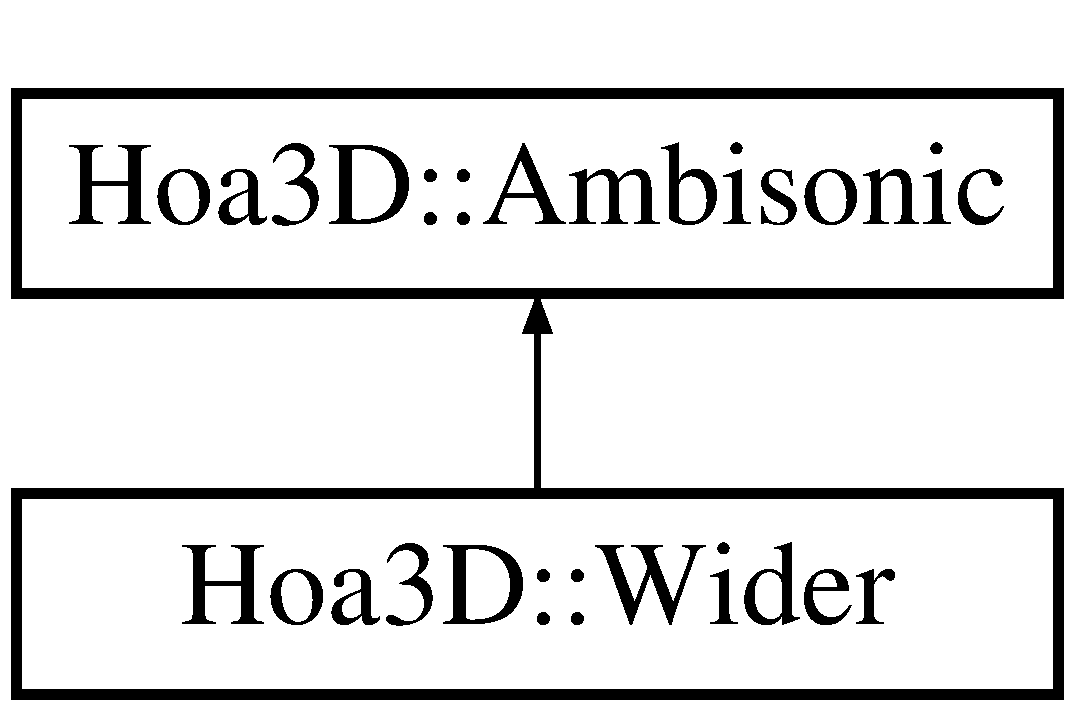
\includegraphics[height=2.000000cm]{class_hoa3_d_1_1_wider}
\end{center}
\end{figure}
\subsection*{Public Member Functions}
\begin{DoxyCompactItemize}
\item 
\hyperlink{class_hoa3_d_1_1_wider_a7f1f80e3329872d06f8e81f60f24e102}{Wider} (unsigned int order)
\begin{DoxyCompactList}\small\item\em The wider constructor. \end{DoxyCompactList}\item 
\hyperlink{class_hoa3_d_1_1_wider_a4a2770414c2753a9c92740f02641db38}{$\sim$\-Wider} ()
\begin{DoxyCompactList}\small\item\em The wider destructor. \end{DoxyCompactList}\item 
void \hyperlink{class_hoa3_d_1_1_wider_a5981d4dafbb0d2ce4ea20ec7cd1fb114}{set\-Widening\-Value} (const double value)
\begin{DoxyCompactList}\small\item\em This method set the widening value. \end{DoxyCompactList}\item 
void \hyperlink{class_hoa3_d_1_1_wider_a605d68c56ca7a541a9e91bd2aa9a9ea0}{process} (const float $\ast$inputs, float $\ast$outputs)
\begin{DoxyCompactList}\small\item\em This method performs the widening with single precision. \end{DoxyCompactList}\item 
void \hyperlink{class_hoa3_d_1_1_wider_a94fa445b540cbafeaafa05d4ed1a20bf}{process} (const double $\ast$inputs, double $\ast$outputs)
\begin{DoxyCompactList}\small\item\em This method performs the widening with double precision. \end{DoxyCompactList}\item 
\hyperlink{class_hoa3_d_1_1_wider_a7f1f80e3329872d06f8e81f60f24e102}{Wider} (unsigned int order)
\begin{DoxyCompactList}\small\item\em The wider constructor. \end{DoxyCompactList}\item 
\hyperlink{class_hoa3_d_1_1_wider_a4a2770414c2753a9c92740f02641db38}{$\sim$\-Wider} ()
\begin{DoxyCompactList}\small\item\em The wider destructor. \end{DoxyCompactList}\item 
void \hyperlink{class_hoa3_d_1_1_wider_a5981d4dafbb0d2ce4ea20ec7cd1fb114}{set\-Widening\-Value} (const double value)
\begin{DoxyCompactList}\small\item\em This method set the widening value. \end{DoxyCompactList}\item 
void \hyperlink{class_hoa3_d_1_1_wider_a605d68c56ca7a541a9e91bd2aa9a9ea0}{process} (const float $\ast$inputs, float $\ast$outputs)
\begin{DoxyCompactList}\small\item\em This method performs the widening with single precision. \end{DoxyCompactList}\item 
void \hyperlink{class_hoa3_d_1_1_wider_a94fa445b540cbafeaafa05d4ed1a20bf}{process} (const double $\ast$inputs, double $\ast$outputs)
\begin{DoxyCompactList}\small\item\em This method performs the widening with double precision. \end{DoxyCompactList}\end{DoxyCompactItemize}


\subsection{Detailed Description}
The ambisonic wider. 

The wider should be used to widen the sound propagation. 

Definition at line 17 of file Wider.\-h.



\subsection{Constructor \& Destructor Documentation}
\hypertarget{class_hoa3_d_1_1_wider_a7f1f80e3329872d06f8e81f60f24e102}{\index{Hoa3\-D\-::\-Wider@{Hoa3\-D\-::\-Wider}!Wider@{Wider}}
\index{Wider@{Wider}!Hoa3D::Wider@{Hoa3\-D\-::\-Wider}}
\subsubsection[{Wider}]{\setlength{\rightskip}{0pt plus 5cm}Hoa3\-D\-::\-Wider\-::\-Wider (
\begin{DoxyParamCaption}
\item[{unsigned int}]{order}
\end{DoxyParamCaption}
)}}\label{class_hoa3_d_1_1_wider_a7f1f80e3329872d06f8e81f60f24e102}


The wider constructor. 

The wider constructor allocates and initialize the member values to computes spherical harmonics weighted coefficients depending of a decomposition order. The order must be at least 1.


\begin{DoxyParams}{Parameters}
{\em order} & The order. \\
\hline
\end{DoxyParams}


Definition at line 11 of file Wider.\-cpp.

\hypertarget{class_hoa3_d_1_1_wider_a4a2770414c2753a9c92740f02641db38}{\index{Hoa3\-D\-::\-Wider@{Hoa3\-D\-::\-Wider}!$\sim$\-Wider@{$\sim$\-Wider}}
\index{$\sim$\-Wider@{$\sim$\-Wider}!Hoa3D::Wider@{Hoa3\-D\-::\-Wider}}
\subsubsection[{$\sim$\-Wider}]{\setlength{\rightskip}{0pt plus 5cm}Hoa3\-D\-::\-Wider\-::$\sim$\-Wider (
\begin{DoxyParamCaption}
{}
\end{DoxyParamCaption}
)}}\label{class_hoa3_d_1_1_wider_a4a2770414c2753a9c92740f02641db38}


The wider destructor. 

The wider destructor free the memory. 

Definition at line 65 of file Wider.\-cpp.

\hypertarget{class_hoa3_d_1_1_wider_a7f1f80e3329872d06f8e81f60f24e102}{\index{Hoa3\-D\-::\-Wider@{Hoa3\-D\-::\-Wider}!Wider@{Wider}}
\index{Wider@{Wider}!Hoa3D::Wider@{Hoa3\-D\-::\-Wider}}
\subsubsection[{Wider}]{\setlength{\rightskip}{0pt plus 5cm}Hoa3\-D\-::\-Wider\-::\-Wider (
\begin{DoxyParamCaption}
\item[{unsigned int}]{order}
\end{DoxyParamCaption}
)}}\label{class_hoa3_d_1_1_wider_a7f1f80e3329872d06f8e81f60f24e102}


The wider constructor. 

The wider constructor allocates and initialize the member values to computes spherical harmonics weighted coefficients depending of a decomposition order. The order must be at least 1.


\begin{DoxyParams}{Parameters}
{\em order} & The order. \\
\hline
\end{DoxyParams}
\hypertarget{class_hoa3_d_1_1_wider_a4a2770414c2753a9c92740f02641db38}{\index{Hoa3\-D\-::\-Wider@{Hoa3\-D\-::\-Wider}!$\sim$\-Wider@{$\sim$\-Wider}}
\index{$\sim$\-Wider@{$\sim$\-Wider}!Hoa3D::Wider@{Hoa3\-D\-::\-Wider}}
\subsubsection[{$\sim$\-Wider}]{\setlength{\rightskip}{0pt plus 5cm}Hoa3\-D\-::\-Wider\-::$\sim$\-Wider (
\begin{DoxyParamCaption}
{}
\end{DoxyParamCaption}
)}}\label{class_hoa3_d_1_1_wider_a4a2770414c2753a9c92740f02641db38}


The wider destructor. 

The wider destructor free the memory. 

\subsection{Member Function Documentation}
\hypertarget{class_hoa3_d_1_1_wider_a605d68c56ca7a541a9e91bd2aa9a9ea0}{\index{Hoa3\-D\-::\-Wider@{Hoa3\-D\-::\-Wider}!process@{process}}
\index{process@{process}!Hoa3D::Wider@{Hoa3\-D\-::\-Wider}}
\subsubsection[{process}]{\setlength{\rightskip}{0pt plus 5cm}void Hoa3\-D\-::\-Wider\-::process (
\begin{DoxyParamCaption}
\item[{const float $\ast$}]{inputs, }
\item[{float $\ast$}]{outputs}
\end{DoxyParamCaption}
)}}\label{class_hoa3_d_1_1_wider_a605d68c56ca7a541a9e91bd2aa9a9ea0}


This method performs the widening with single precision. 

You should use this method for in-\/place or not-\/in-\/place processing and performs the widening sample by sample. The inputs array and outputs array contains the spherical harmonics samples and the minimum size must be the number of harmonics.


\begin{DoxyParams}{Parameters}
{\em inputs} & The input array. \\
\hline
{\em outputs} & The output array. \\
\hline
\end{DoxyParams}


Definition at line 53 of file Wider.\-cpp.

\hypertarget{class_hoa3_d_1_1_wider_a605d68c56ca7a541a9e91bd2aa9a9ea0}{\index{Hoa3\-D\-::\-Wider@{Hoa3\-D\-::\-Wider}!process@{process}}
\index{process@{process}!Hoa3D::Wider@{Hoa3\-D\-::\-Wider}}
\subsubsection[{process}]{\setlength{\rightskip}{0pt plus 5cm}void Hoa3\-D\-::\-Wider\-::process (
\begin{DoxyParamCaption}
\item[{const float $\ast$}]{inputs, }
\item[{float $\ast$}]{outputs}
\end{DoxyParamCaption}
)}}\label{class_hoa3_d_1_1_wider_a605d68c56ca7a541a9e91bd2aa9a9ea0}


This method performs the widening with single precision. 

You should use this method for in-\/place or not-\/in-\/place processing and performs the widening sample by sample. The inputs array and outputs array contains the spherical harmonics samples and the minimum size must be the number of harmonics.


\begin{DoxyParams}{Parameters}
{\em inputs} & The input array. \\
\hline
{\em outputs} & The output array. \\
\hline
\end{DoxyParams}
\hypertarget{class_hoa3_d_1_1_wider_a94fa445b540cbafeaafa05d4ed1a20bf}{\index{Hoa3\-D\-::\-Wider@{Hoa3\-D\-::\-Wider}!process@{process}}
\index{process@{process}!Hoa3D::Wider@{Hoa3\-D\-::\-Wider}}
\subsubsection[{process}]{\setlength{\rightskip}{0pt plus 5cm}void Hoa3\-D\-::\-Wider\-::process (
\begin{DoxyParamCaption}
\item[{const double $\ast$}]{inputs, }
\item[{double $\ast$}]{outputs}
\end{DoxyParamCaption}
)}}\label{class_hoa3_d_1_1_wider_a94fa445b540cbafeaafa05d4ed1a20bf}


This method performs the widening with double precision. 

You should use this method for in-\/place or not-\/in-\/place processing and performs the widening sample by sample. The inputs array and outputs array contains the spherical harmonics samples and the minimum size must be the number of harmonics.


\begin{DoxyParams}{Parameters}
{\em inputs} & The input array. \\
\hline
{\em outputs} & The output array. \\
\hline
\end{DoxyParams}
\hypertarget{class_hoa3_d_1_1_wider_a94fa445b540cbafeaafa05d4ed1a20bf}{\index{Hoa3\-D\-::\-Wider@{Hoa3\-D\-::\-Wider}!process@{process}}
\index{process@{process}!Hoa3D::Wider@{Hoa3\-D\-::\-Wider}}
\subsubsection[{process}]{\setlength{\rightskip}{0pt plus 5cm}void Hoa3\-D\-::\-Wider\-::process (
\begin{DoxyParamCaption}
\item[{const double $\ast$}]{inputs, }
\item[{double $\ast$}]{outputs}
\end{DoxyParamCaption}
)}}\label{class_hoa3_d_1_1_wider_a94fa445b540cbafeaafa05d4ed1a20bf}


This method performs the widening with double precision. 

You should use this method for in-\/place or not-\/in-\/place processing and performs the widening sample by sample. The inputs array and outputs array contains the spherical harmonics samples and the minimum size must be the number of harmonics.


\begin{DoxyParams}{Parameters}
{\em inputs} & The input array. \\
\hline
{\em outputs} & The output array. \\
\hline
\end{DoxyParams}


Definition at line 59 of file Wider.\-cpp.

\hypertarget{class_hoa3_d_1_1_wider_a5981d4dafbb0d2ce4ea20ec7cd1fb114}{\index{Hoa3\-D\-::\-Wider@{Hoa3\-D\-::\-Wider}!set\-Widening\-Value@{set\-Widening\-Value}}
\index{set\-Widening\-Value@{set\-Widening\-Value}!Hoa3D::Wider@{Hoa3\-D\-::\-Wider}}
\subsubsection[{set\-Widening\-Value}]{\setlength{\rightskip}{0pt plus 5cm}void Hoa3\-D\-::\-Wider\-::set\-Widening\-Value (
\begin{DoxyParamCaption}
\item[{const double}]{value}
\end{DoxyParamCaption}
)}}\label{class_hoa3_d_1_1_wider_a5981d4dafbb0d2ce4ea20ec7cd1fb114}


This method set the widening value. 

The widening value is clipped between 0 and 1. At 1, the sound field has no changes. At 0, all the sound field is omni directionnal.


\begin{DoxyParams}{Parameters}
{\em value} & The widening value. \\
\hline
\end{DoxyParams}
\hypertarget{class_hoa3_d_1_1_wider_a5981d4dafbb0d2ce4ea20ec7cd1fb114}{\index{Hoa3\-D\-::\-Wider@{Hoa3\-D\-::\-Wider}!set\-Widening\-Value@{set\-Widening\-Value}}
\index{set\-Widening\-Value@{set\-Widening\-Value}!Hoa3D::Wider@{Hoa3\-D\-::\-Wider}}
\subsubsection[{set\-Widening\-Value}]{\setlength{\rightskip}{0pt plus 5cm}void Hoa3\-D\-::\-Wider\-::set\-Widening\-Value (
\begin{DoxyParamCaption}
\item[{const double}]{value}
\end{DoxyParamCaption}
)}}\label{class_hoa3_d_1_1_wider_a5981d4dafbb0d2ce4ea20ec7cd1fb114}


This method set the widening value. 

The widening value is clipped between 0 and 1. At 1, the sound field has no changes. At 0, all the sound field is omni directionnal.


\begin{DoxyParams}{Parameters}
{\em value} & The widening value. \\
\hline
\end{DoxyParams}


Definition at line 48 of file Wider.\-cpp.



The documentation for this class was generated from the following files\-:\begin{DoxyCompactItemize}
\item 
/\-Users/elioton/\-Documents/programmation/\-C\-I\-C\-M/source\-Tree/\-Hoa\-Library/\-Sources/\-Hoa3\-D/Wider.\-h\item 
/\-Users/elioton/\-Documents/programmation/\-C\-I\-C\-M/source\-Tree/\-Hoa\-Library/\-Sources/hoa\-Wider/Hoa3\-D\-Wider.\-h\item 
/\-Users/elioton/\-Documents/programmation/\-C\-I\-C\-M/source\-Tree/\-Hoa\-Library/\-Sources/\-Hoa3\-D/Wider.\-cpp\item 
/\-Users/elioton/\-Documents/programmation/\-C\-I\-C\-M/source\-Tree/\-Hoa\-Library/\-Sources/hoa\-Wider/Hoa3\-D\-Wider.\-cpp\end{DoxyCompactItemize}

%--- End generated contents ---

% Index
\newpage
\phantomsection
\addcontentsline{toc}{part}{Index}
\printindex

\end{document}
